%Page Setup, don't remove
\documentclass[12pt]{book} 
\setlength{\columnsep}{0.7truecm}
\setlength{\parindent}{0cm}
\usepackage[top=2truecm,bottom=2.8truecm, left=2.2truecm, right=2.2truecm,headsep=10pt, paperwidth=19.3truecm, paperheight=27.6truecm]{geometry} 
\usepackage[usenames,dvipsnames]{xcolor}
\usepackage{tcolorbox}
\definecolor{ocre}{RGB}{52,177,201} 
\usepackage{pdfpages}
\usepackage{avant}
\usepackage{bussproofs}
\usepackage{mathptmx}
%\usepackage{ebgaramond}
 \usepackage{xeCJK}
 \setCJKmainfont{SimSun}
\usepackage{tikz}
\usepackage{tkz-euclide}
\usepackage{matchsticks}
\usepackage{wrapfig}
\usepackage{listings}
\usepackage[utf8]{vietnam}
\usepackage{babel}
\usepackage[LSBC5,T1]{fontenc}

%----------------------------------------------------------------------------------------
%	VARIOUS REQUIRED PACKAGES
%----------------------------------------------------------------------------------------
\usepackage{titlesec} % Allows customization of titles
\usepackage{multicol}
\usepackage{graphicx} % Required for including pictures
%\graphicspath{{Pictures/}} % Specifies the directory where pictures are stored
\usepackage{lipsum} % Inserts dummy text
\usepackage{tikz} % Required for drawing custom shapes
%\usepackage{enumitem} % Customize lists
%\setlist{nolistsep} % Reduce spacing between bullet points and numbered lists
\usepackage{booktabs} % Required for nicer horizontal rules in tables
\usepackage{eso-pic} % Required for specifying an image background in the title page
\usepackage{titletoc} % Required for manipulating the table of contents
\contentsmargin{0cm} % Removes the default margin
\usepackage{adjustbox} 
\usepackage{amsmath,amsfonts,amssymb,amsthm} % For math equations, theorems, symbols, etc
%\usepackage[framemethod=tikz]{mdframed} 
\usepackage[sexy]{evan}
\usepackage{hyperref}
\urlstyle{same}
\usepackage{tikz} % figure in two column
\usepackage{float}
\usepackage{biblatex}
\usepackage{caption}% dinh dang figure caption
%\usepackage[font=normalsize]{caption}
\usepackage{changepage}
\usepackage{booktabs}

\usepackage{chngcntr}
\usepackage{array}
\usepackage{eurosym}
\usepackage{multirow}
\usepackage{mathtools}
\usepackage{setspace}
\usepackage{afterpage}
\usepackage{scalerel}
\usepackage{blindtext}
\usepackage{tabularx}
\usepackage{afterpage}
\usepackage{array}
%\usepackage{transparent}
\usepackage{efbox}
\usepackage{tabulary}
% \usepackage{CJKutf8}
\usepackage{subcaption}
\usepackage{rotating}
\usepackage{microtype}
\usepackage{pgfplots}

\usetikzlibrary{lindenmayersystems}
\usetikzlibrary{shapes,shapes.geometric}
\usetikzlibrary{decorations.pathreplacing}
\usetikzlibrary{calc,intersections}
\usetikzlibrary[shadings]
\usetikzlibrary{decorations.fractals}

\newmdenv[skipabove=7pt,
skipbelow=7pt,
backgroundcolor=black!5,
linecolor=ocre,
leftline=true,
innerleftmargin=6pt,
innerrightmargin=6pt,
innertopmargin=8pt,
leftmargin=0cm,
rightmargin=0cm,
innerbottommargin=8pt]{tBox}

\def\PIbox#1{\tikz\node[draw = ocre,fill=black!5,align=justify,text width=.95\linewidth,inner sep=2mm]{#1};}%
\renewcommand{\qedsymbol}{}	
\usepackage{fancyhdr} % Required for header and footer configuration
%%%% Header for duong vao toan hoc
\fancypagestyle{duongvaotoanhoc}{
	\fancyhf{}
	\fancyhead[E]{
		\insertpic{63}{740}{1}{duongvao1}
		\insertpic{333}{35}{1}{fduongvao1}
}
	\fancyhead[O]{
		\insertpic{1}{740}{1}{duongvao2}
		\insertpic{59}{34.9}{1}{fduongvao2}
}	
\renewcommand{\footrulewidth}{0pt}
\fancyfoot[LE,RO]{\sffamily\footnotesize	\thepage}

\fancyfoot[LO,RE]{\sffamily\scriptsize TẬP 7 -- SỐ 3 THÁNG 3/2023}
}

\fancypagestyle{duongvaotoanhocnone}{
	\fancyhf{}
	\fancyhead[E]{
		\insertpic{333}{35}{1}{fduongvao1}
	}
	\fancyhead[O]{
		\insertpic{59}{34.9}{1}{fduongvao2}
	}	
	\renewcommand{\footrulewidth}{0pt}
	\fancyfoot[LE,RO]{\sffamily\footnotesize	\thepage}
	
	\fancyfoot[LO,RE]{\sffamily\scriptsize TẬP 7 -- SỐ 3 THÁNG 3/2023}
}

\fancypagestyle{thachthuctoanhoc}{
	\fancyhf{}
	\fancyhead[E]{
		\insertpic{63}{740}{1}{thachthuc1}
		\insertpic{333}{35}{1}{fthachthuc1}
	}
	\fancyhead[O]{
		\insertpic{1}{740}{1}{thachthuc2}
		\insertpic{59}{34.9}{1}{fthachthuc2}
	}	
	\renewcommand{\footrulewidth}{0pt}
	\fancyfoot[LE,RO]{\sffamily\footnotesize	\thepage}
	
	\fancyfoot[LO,RE]{\sffamily\scriptsize TẬP 7 -- SỐ 3 THÁNG 3/2023}
}

\fancypagestyle{thachthuctoanhocnone}{
	\fancyhf{}
	\fancyhead[E]{
		\insertpic{333}{35}{1}{fthachthuc1}
	}
	\fancyhead[O]{
		\insertpic{59}{34.9}{1}{fthachthuc2}
	}	
	\renewcommand{\footrulewidth}{0pt}
	\fancyfoot[LE,RO]{\sffamily\footnotesize	\thepage}
	
	\fancyfoot[LO,RE]{\sffamily\scriptsize TẬP 7 -- SỐ 3 THÁNG 3/2023}
}


%%%% Header for Toán học và đời sống
\fancypagestyle{toanhocvadoisong}{
			\fancyhf{}
		\fancyhead[E]{
			\insertpic{63}{740}{1}{toanhocds1}
			\insertpic{333}{35}{1}{ftoanhocds1}
		}
		\fancyhead[O]{
			\insertpic{1}{740}{1}{toanhocds2}
			\insertpic{59}{34.9}{1}{ftoanhocds2}
		}	
		\renewcommand{\footrulewidth}{0pt}
		\fancyfoot[LE,RO]{\sffamily\footnotesize	\thepage}
		
		\fancyfoot[LO,RE]{\sffamily\scriptsize TẬP 7 -- SỐ 3 THÁNG 3/2023}
}
\fancypagestyle{toanhocvadoisongnone}{
	\fancyhf{}
	\fancyhead[E]{
		\insertpic{333}{35}{1}{ftoanhocds1}
	}
	\fancyhead[O]{
		\insertpic{59}{34.9}{1}{ftoanhocds2}
	}	
	\renewcommand{\footrulewidth}{0pt}
	\fancyfoot[LE,RO]{\sffamily\footnotesize	\thepage}
	
	\fancyfoot[LO,RE]{\sffamily\scriptsize TẬP 7 -- SỐ 3 THÁNG 3/2023}
}

\fancypagestyle{doisongtoanhoc}{
	\fancyhf{}
	\fancyhead[E]{
		\insertpic{63}{740}{1}{dstoanhoc1}
		\insertpic{333}{35}{1}{fdstoanhoc1}
	}
	\fancyhead[O]{
		\insertpic{1}{740}{1}{dstoanhoc2}
		\insertpic{59}{34.9}{1}{fdstoanhoc2}
	}	
	\renewcommand{\footrulewidth}{0pt}
	\fancyfoot[LE,RO]{\sffamily\footnotesize	\thepage}
	
	\fancyfoot[LO,RE]{\sffamily\scriptsize TẬP 7 -- SỐ 3 THÁNG 3/2023}
}
\fancypagestyle{doisongtoanhocnone}{
	\fancyhf{}
	\fancyhead[E]{
		\insertpic{333}{35}{1}{fdstoanhoc1}
	}
	\fancyhead[O]{
		\insertpic{59}{34.9}{1}{fdstoanhoc2}
	}	
	\renewcommand{\footrulewidth}{0pt}
	\fancyfoot[LE,RO]{\sffamily\footnotesize	\thepage}
	
	\fancyfoot[LO,RE]{\sffamily\scriptsize TẬP 7 -- SỐ 3 THÁNG 3/2023}
}

%%% doi thoai toan hoc
\fancypagestyle{doithoaitoanhoc}{
	\fancyhf{}
	\fancyhead[E]{
		\insertpic{63}{740}{1}{doithoai1}
		\insertpic{333}{35}{1}{fdoithoai1}
	}
	\fancyhead[O]{
		\insertpic{1}{740}{1}{doithoai2}
		\insertpic{59}{34.9}{1}{fdoithoai2}
	}	
	\renewcommand{\footrulewidth}{0pt}
	\fancyfoot[LE,RO]{\sffamily\footnotesize	\thepage}
	
	\fancyfoot[LO,RE]{\sffamily\scriptsize TẬP 7 -- SỐ 3 THÁNG 3/2023}
}
\fancypagestyle{doithoaitoanhocnone}{
	\fancyhf{}
	\fancyhead[E]{
		\insertpic{333}{35}{1}{fdoithoai1}
	}
	\fancyhead[O]{
		\insertpic{59}{34.9}{1}{fdoithoai2}
	}	
	\renewcommand{\footrulewidth}{0pt}
	\fancyfoot[LE,RO]{\sffamily\footnotesize	\thepage}
	
	\fancyfoot[LO,RE]{\sffamily\scriptsize TẬP 7 -- SỐ 3 THÁNG 3/2023}
}

%%%% Header for co dien hien dai
\fancypagestyle{codienhiendai}{
	\fancyhf{}
	\fancyhead[E]{
		\insertpic{63}{740}{1}{codien1}
		\insertpic{333}{35}{1}{fcodien1}
	}
	\fancyhead[O]{
		\insertpic{1}{740}{1}{codien2}
		\insertpic{59}{34.9}{1}{fcodien2}
	}	
	\renewcommand{\footrulewidth}{0pt}
	\fancyfoot[LE,RO]{\sffamily\footnotesize	\thepage}
	
	\fancyfoot[LO,RE]{\sffamily\scriptsize TẬP 7 -- SỐ 3 THÁNG 3/2023}
}
\fancypagestyle{codienhiendainone}{
	\fancyhf{}
	\fancyhead[E]{
		\insertpic{333}{35}{1}{fcodien1}
	}
	\fancyhead[O]{
		\insertpic{59}{34.9}{1}{fcodien2}
	}	
	\renewcommand{\footrulewidth}{0pt}
	\fancyfoot[LE,RO]{\sffamily\footnotesize	\thepage}
	
	\fancyfoot[LO,RE]{\sffamily\scriptsize TẬP 7 -- SỐ 3 THÁNG 3/2023}
}

\fancypagestyle{diendandayvahoctoan}{
	\fancyhf{}
	\fancyhead[E]{
		\insertpic{63}{740}{1}{diendan1}
		\insertpic{333}{35}{1}{fdiendan1}
	}
	\fancyhead[O]{
		\insertpic{1}{740}{1}{diendan2}
		\insertpic{59}{34.9}{1}{fdiendan2}
	}	
	\renewcommand{\footrulewidth}{0pt}
	\fancyfoot[LE,RO]{\sffamily\footnotesize	\thepage}
	
	\fancyfoot[LO,RE]{\sffamily\scriptsize TẬP 7 -- SỐ 3 THÁNG 3/2023}
}
\fancypagestyle{diendandayvahoctoannone}{
	\fancyhf{}
	\fancyhead[E]{
		\insertpic{333}{35}{1}{fdiendan1}
	}
	\fancyhead[O]{
		\insertpic{59}{34.9}{1}{fdiendan2}
	}	
	\renewcommand{\footrulewidth}{0pt}
	\fancyfoot[LE,RO]{\sffamily\footnotesize	\thepage}
	
	\fancyfoot[LO,RE]{\sffamily\scriptsize TẬP 7 -- SỐ 3 THÁNG 3/2023}
}

\fancypagestyle{cackithitoan}{
	\fancyhf{}
	\fancyhead[E]{
		\insertpic{63}{740}{1}{cackithi1}
		\insertpic{333}{35}{1}{fcackithi1}
	}
	\fancyhead[O]{
		\insertpic{1}{740}{1}{cackithi2}
		\insertpic{59}{34.9}{1}{fcackithi2}
	}	
	\renewcommand{\footrulewidth}{0pt}
	\fancyfoot[LE,RO]{\sffamily\footnotesize	\thepage}
	
	\fancyfoot[LO,RE]{\sffamily\scriptsize TẬP 7 -- SỐ 3 THÁNG 3/2023}
}
\fancypagestyle{cackithitoannone}{
	\fancyhf{}
	\fancyhead[E]{
		\insertpic{333}{35}{1}{fcackithi1}
	}
	\fancyhead[O]{
		\insertpic{59}{34.9}{1}{fcackithi2}
	}	
	\renewcommand{\footrulewidth}{0pt}
	\fancyfoot[LE,RO]{\sffamily\footnotesize	\thepage}
	
	\fancyfoot[LO,RE]{\sffamily\scriptsize TẬP 7 -- SỐ 3 THÁNG 3/2023}
}

\fancypagestyle{lichsutoanhoc}{
	\fancyhf{}
	\fancyhead[E]{
		\insertpic{63}{740}{1}{lichsu1}
		\insertpic{333}{35}{1}{flichsu1}
	}
	\fancyhead[O]{
		\insertpic{1}{740}{1}{lichsu2}
		\insertpic{59}{34.9}{1}{flichsu2}
	}	
	\renewcommand{\footrulewidth}{0pt}
	\fancyfoot[LE,RO]{\sffamily\footnotesize	\thepage}
	
	\fancyfoot[LO,RE]{\sffamily\scriptsize TẬP 7 -- SỐ 3 THÁNG 3/2023}
}
\fancypagestyle{lichsutoanhocnone}{
	\fancyhf{}
	\fancyhead[E]{
		\insertpic{333}{35}{1}{flichsu1}
	}
	\fancyhead[O]{
		\insertpic{59}{34.9}{1}{flichsu2}
	}	
	\renewcommand{\footrulewidth}{0pt}
	\fancyfoot[LE,RO]{\sffamily\footnotesize	\thepage}
	
	\fancyfoot[LO,RE]{\sffamily\scriptsize TẬP 7 -- SỐ 3 THÁNG 3/2023}
}

%%%% Header for Tìm hiểu khoa học
\fancypagestyle{timhieukhoahoc}{
		\fancyhf{}
	\fancyhead[E]{
		\insertpic{63}{740}{1}{timhieu1}
		\insertpic{333}{35}{1}{ftimhieu1}
	}
	\fancyhead[O]{
		\insertpic{1}{740}{1}{timhieu2}
		\insertpic{59}{34.9}{1}{ftimhieu2}
	}	
	\renewcommand{\footrulewidth}{0pt}
	\fancyfoot[LE,RO]{\sffamily\footnotesize	\thepage}
	
	\fancyfoot[LO,RE]{\sffamily\scriptsize TẬP 7 -- SỐ 3 THÁNG 3/2023}	
}
\fancypagestyle{timhieukhoahocnone}{
	\fancyhf{}
	\fancyhead[E]{
		\insertpic{333}{35}{1}{ftimhieu1}
	}
	\fancyhead[O]{
		\insertpic{59}{34.9}{1}{ftimhieu2}
	}	
	\renewcommand{\footrulewidth}{0pt}
	\fancyfoot[LE,RO]{\sffamily\footnotesize	\thepage}
	
	\fancyfoot[LO,RE]{\sffamily\scriptsize TẬP 7 -- SỐ 3 THÁNG 3/2023}	
}

%%%% Header for quan toan
\fancypagestyle{quantoan}{
		\fancyhf{}
		\fancyhead[E]{
		\insertpic{63}{740}{1}{quantoan1}
		\insertpic{333}{35}{1}{fquantoan1}
	}
	\fancyhead[O]{
		\insertpic{1}{740}{1}{quantoan2}
		\insertpic{59}{34.9}{1}{fquantoan2}
	}	
	\renewcommand{\footrulewidth}{0pt}
	\fancyfoot[LE,RO]{\sffamily\footnotesize	\thepage}
	
	\fancyfoot[LO,RE]{\sffamily\scriptsize TẬP 7 -- SỐ 3 THÁNG 3/2023}
}
\fancypagestyle{quantoannone}{
	\fancyhf{}
	\fancyhead[E]{
		\insertpic{333}{35}{1}{fquantoan1}
	}
	\fancyhead[O]{
		\insertpic{59}{34.9}{1}{fquantoan2}
	}	
	\renewcommand{\footrulewidth}{0pt}
	\fancyfoot[LE,RO]{\sffamily\footnotesize	\thepage}
	
	\fancyfoot[LO,RE]{\sffamily\scriptsize TẬP 7 -- SỐ 3 THÁNG 3/2023}
}


\fancypagestyle{hoccungpi}{
				\fancyhf{}
		\fancyhead[E]{
			\insertpic{63}{740}{1}{hoccungpi1}
			\insertpic{333}{35}{1}{fhoccungpi1}
		}
		\fancyhead[O]{
			\insertpic{1}{740}{1}{hoccungpi2}
			\insertpic{59}{34.9}{1}{fhoccungpi2}
		}	
		\renewcommand{\footrulewidth}{0pt}
		\fancyfoot[LE,RO]{\sffamily\footnotesize	\thepage}
		
		\fancyfoot[LO,RE]{\sffamily\scriptsize TẬP 7 -- SỐ 3 THÁNG 3/2023}	
}
\fancypagestyle{hoccungpinone}{
	\fancyhf{}
	\fancyhead[E]{
		\insertpic{333}{35}{1}{fhoccungpi1}
	}
	\fancyhead[O]{
		\insertpic{59}{34.9}{1}{fhoccungpi2}
	}	
	\renewcommand{\footrulewidth}{0pt}
	\fancyfoot[LE,RO]{\sffamily\footnotesize	\thepage}
	
	\fancyfoot[LO,RE]{\sffamily\scriptsize TẬP 7 -- SỐ 3 THÁNG 3/2023}	
}

\fancypagestyle{toancuabi}{
	\fancyhf{}
	\fancyhead[E]{
		\insertpic{63}{740}{1}{toancuabi1}
		\insertpic{333}{35}{1}{ftoancuabi1}
	}
	\fancyhead[O]{
		\insertpic{1}{740}{1}{toancuabi2}
		\insertpic{59}{34.9}{1}{ftoancuabi2}
	}	
	\renewcommand{\footrulewidth}{0pt}
	\fancyfoot[LE,RO]{\sffamily\footnotesize	\thepage}
	
	\fancyfoot[LO,RE]{\sffamily\scriptsize TẬP 7 -- SỐ 3 THÁNG 3/2023}	
}
\fancypagestyle{toancuabinone}{
	\fancyhf{}
	\fancyhead[E]{
		\insertpic{333}{35}{1}{ftoancuabi1}
	}
	\fancyhead[O]{
		\insertpic{59}{34.9}{1}{ftoancuabi2}
	}	
	\renewcommand{\footrulewidth}{0pt}
	\fancyfoot[LE,RO]{\sffamily\footnotesize	\thepage}
	
	\fancyfoot[LO,RE]{\sffamily\scriptsize TẬP 7 -- SỐ 3 THÁNG 3/2023}	
}

\fancypagestyle{gocco}{
	\fancyhf{}
	\fancyhead[E]{
		\insertpic{63}{740}{1}{gocco1}
		\insertpic{333}{35}{1}{fgocco1}
	}
	\fancyhead[O]{
		\insertpic{1}{740}{1}{gocco2}
		\insertpic{59}{34.9}{1}{fgocco2}
	}	
	\renewcommand{\footrulewidth}{0pt}
	\fancyfoot[LE,RO]{\sffamily\footnotesize	\thepage}
	
	\fancyfoot[LO,RE]{\sffamily\scriptsize TẬP 7 -- SỐ 3 THÁNG 3/2023}	
}

\fancypagestyle{gocconone}{
	\fancyhf{}
	\fancyhead[E]{
		\insertpic{333}{35}{1}{fgocco1}
	}
	\fancyhead[O]{
		\insertpic{59}{34.9}{1}{fgocco2}
	}	
	\renewcommand{\footrulewidth}{0pt}
	\fancyfoot[LE,RO]{\sffamily\footnotesize	\thepage}
	
	\fancyfoot[LO,RE]{\sffamily\scriptsize TẬP 7 -- SỐ 3 THÁNG 3/2023}	
}
	
%	\fancyfoot[C]{\sffamily\footnotesize Tạp chí Pi } % Print the nearest section name on the left side of odd pages	


\pagestyle{fancy}
\renewcommand{\chaptermark}[1]{\markboth{\normalsize\bfseries\chaptername\ \thechapter.\ #1}{}} % Chapter text font settings
\renewcommand{\sectionmark}[1]{\markright{\normalsize\thesection\hspace{5pt}#1}{}} % Section text font settings


\fancyfoot[LE,RO]{\sffamily\footnotesize	\thepage} % Font setting for the page number in the header
\fancyfoot[LO,RE]{\sffamily\footnotesize TẬP 7 -- SỐ 3 THÁNG 3/2023 \LARGE  $\pmb{\pi}$}


\fancyfoot[C]{\sffamily\footnotesize Tạp chí Pi } % Print the nearest section name on the left side of odd pages
\renewcommand{\headrulewidth}{0pt} % Width of the rule under the header
\addtolength{\headheight}{2.5pt} % Increase the spacing around the header slightly
\renewcommand{\footrulewidth}{.5pt} % Removes the rule in the footer


\fancypagestyle{plain}{\fancyhead{}\renewcommand{\headrulewidth}{0pt}} % Style for when a plain pagestyle is specified

% Removes the header from odd empty pages at the end of chapters
\makeatletter
\renewcommand{\cleardoublepage}{
	\clearpage\ifodd\c@page\else
	\hbox{}
	\vspace*{\fill}
	\thispagestyle{empty}
	\newpage
	\fi}


\graphicspath{{../main/pic/}}
\everymath{\displaystyle}
\DeclareMathAlphabet{\pazocal}{OMS}{zplm}{m}{n}
\usepackage{ebgaramond}
\usepackage{xpatch}
\PassOptionsToPackage{hyphens}{url}

\usepackage{url}
\usepackage{type1cm}
\usepackage{lettrine}
\usepackage{makecell}
\renewcommand{\LettrineTextFont}{\rmfamily}
\usepackage{skak}
%\usepackage{xskak}
\usepackage{tabularx}
\usepackage{microtype}
\usepackage{cases}
\usepackage{tikz-cd}
\usepackage{oplotsymbl}
\definecolor{codienhiendai}{cmyk}{0.72, 0, 0.42, 0.1}
\definecolor{thachthuctoanhoc}{cmyk}{0.87, 0.46, 0.69, 0.31}
\definecolor{diendantoanhoc}{cmyk}{0.75, 0, 0.7, 0}
\definecolor{timhieukhoahoc}{cmyk}{0.84, 0.7, 0, 0}
\definecolor{quantoan}{cmyk}{0.8, 0.57, 0, 0}
\definecolor{cackithi}{cmyk}{0.7, 0.35, 0, 0}
\definecolor{hoccungpi}{cmyk}{0.67, 0.6, 0, 0}
\definecolor{gocco}{cmyk}{0.65, 0.78, 0, 0}
\definecolor{toancuabi}{cmyk}{0, 1, 0, 0}
\definecolor{doithoaitoanhoc}{cmyk}{0.6, 0.3, 0 ,0.63}
\definecolor{duongvaotoanhoc}{cmyk}{0, 0.7, 0.9, 0}
\definecolor{toanhocdoisong}{cmyk}{0 , 0.93, 1, 0}
\definecolor{tramthienvan}{cmyk}{0, 0.98, 0.95, 0}
\definecolor{lichsutoanhoc}{cmyk}{0.35, 0.5, 0.8, 0.1}
\definecolor{doisongtoanhoc}{cmyk}{0.25, 0.3, 0.5, 0.1}
\definecolor{amber}{rgb}{1.0, 0.75, 0.0}

\definecolor{darkblue}{rgb}{0.089,0.21,0.363}
\usepackage[hang,splitrule]{footmisc}
\usetikzlibrary{arrows}
\usetikzlibrary{patterns}
\usetikzlibrary{decorations.pathreplacing,calligraphy,backgrounds}
\setlength{\footnotemargin}{0cm}
\setlength{\footnotesep}{0.35cm}
\setlength{\skip\footins}{0.35cm}
\setlength\footskip{33pt}

\newcommand\blfootnote[1]{%
	\begingroup
	\renewcommand\thefootnote{}\footnote{#1}%
	\addtocounter{footnote}{-1}%
	\endgroup
}

\def\footnotelayout{\itshape}
\renewcommand*\footnoterule{}
\renewcommand\footnoterule{\vspace*{0.25cm}\hrule width 1\textwidth\vspace*{0.25cm}}

\newcommand{\insertpic}[4]{
	\begingroup
	\AddToShipoutPicture*{\put(#1,#2){\includegraphics[scale=#3]{#4}}} % %Image background
	\centering
	\endgroup
}

\tikzset{
	squarednode/.style={rectangle, draw=red!60, fill=red!5, very thick, minimum size=3mm}
}

\tikzset{
	sqnode/.style={rectangle, draw=cackithi, very thick, minimum size=3mm}
}

\tikzset{
	roundnode/.style={circle, draw=toancuabi, fill=cackithi!50, minimum size=3mm},
}


\begin{document}
%	 \thispagestyle{empty}
%	 \begingroup 
%	 \AddToShipoutPicture*{\put(0,0){\includegraphics[scale=1]{ML.pdf}}}
%	 \centering
%	 \vspace*{0cm}
%	 \endgroup
%	 \newpage	  
%	 \pagestyle{empty}
%
%	\thispagestyle{empty}
%	\begingroup 
%	\AddToShipoutPicture*{\put(0,0){
\includegraphics[scale=1]{CMNM.pdf}}}
%	\centering
%	\vspace*{0cm}
%	\endgroup
%	\newpage	
%	\pagestyle{empty}
%	
%	\setcounter{page}{3}
%	
%	\setcounter{figure}{0}
%	\thispagestyle{toanhocvadoisongnone}
\pagestyle{toanhocvadoisong}
\everymath{\color{toanhocdoisong}}
\graphicspath{{../toanhocdoisong/pic2/}}
\blfootnote{$^1$\color{toanhocdoisong}Hà Nội.}
\begingroup
\AddToShipoutPicture*{\put(0,616){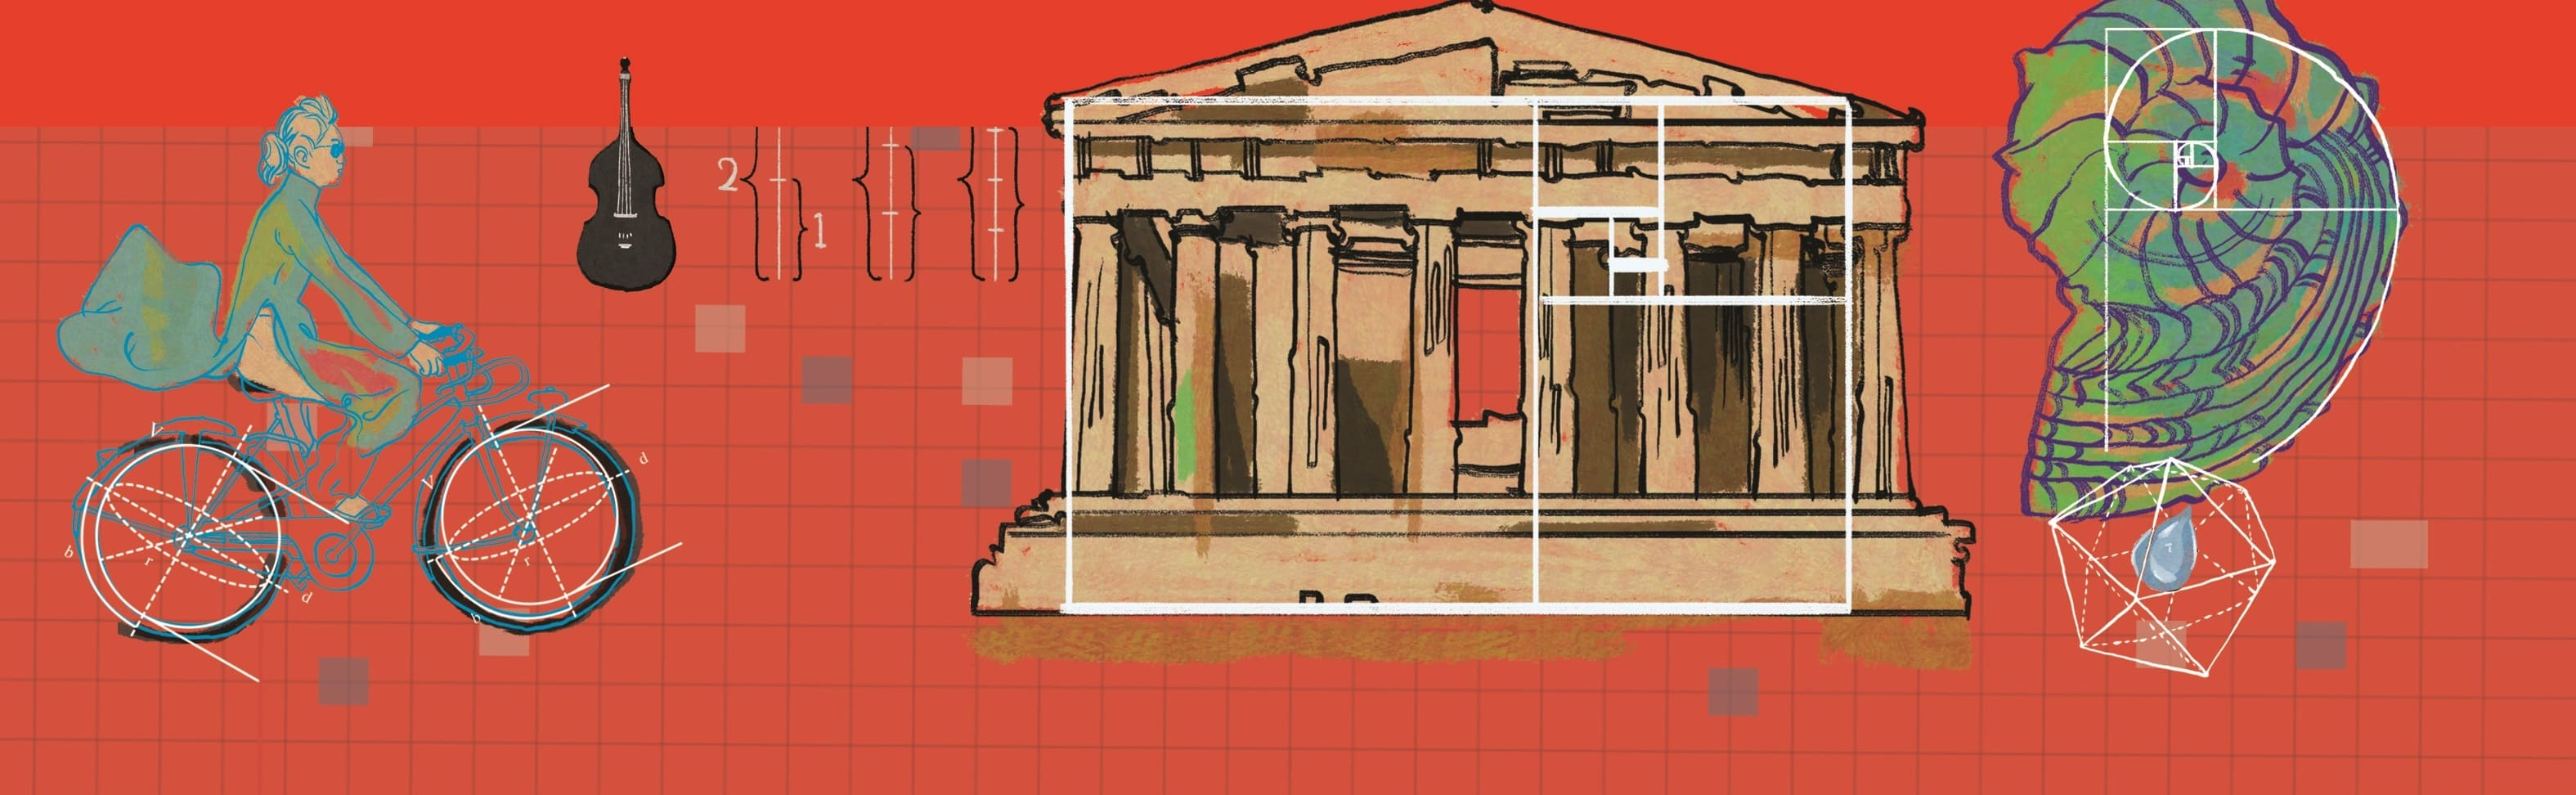
\includegraphics[width=19.3cm]{../bannertoanhocdoisong}}}
\AddToShipoutPicture*{\put(137,523){
\includegraphics[scale=1]{../tieude2.pdf}}}
\centering
\endgroup

\vspace*{185pt}
\begin{multicols}{2}
	Gắn liền với sự phát triển của hình học, nghề trắc địa cũng xuất hiện rất sớm trong lịch sử nhân loại, từ nhiều nghìn năm trước. Đặc biệt, đến thời La Mã cổ đại, nó đóng một vai trò quan trọng trong nhiều mặt của xã hội. Trong bài viết này, chúng ta hãy cùng tìm hiểu về các công cụ và phương pháp đo đạc cũng như những thành tựu còn lưu lại của trắc địa La Mã.
	\vskip 0.1cm
	$\pmb{1.}$ \textbf{\color{toanhocdoisong}Các dụng cụ trắc địa}
	\begin{figure}[H]
		\vspace*{-5pt}
		\centering
		\captionsetup{labelformat= empty, justification=centering}
		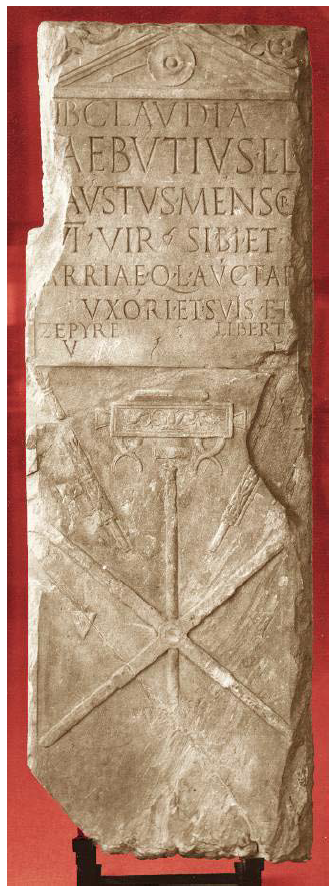
\includegraphics[height=0.8\linewidth]{1a}
		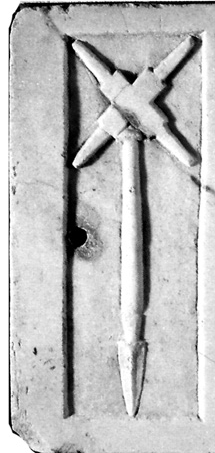
\includegraphics[height=0.8\linewidth]{1b}
		\caption{\small\textit{\color{toanhocdoisong}Hình $1$. Hình khắc groma trên bia mộ của những người làm trắc địa thời La Mã.}}
		\vspace*{-10pt}
	\end{figure}
	Ngoài các dụng cụ cơ bản thường thấy như cọc và dây thừng, dụng cụ trắc địa mang tính biểu tượng nhất của người La Mã là một thiết bị mang tên \textit{groma}. Nó xuất hiện phổ biến trong nhiều tài liệu trắc địa còn sót lại cũng như trên bia mộ của những nhà trắc địa La Mã. Từ hiện vật phát hiện được ở di chỉ Pompeii và các mô tả bằng lời trên văn bản, cấu tạo của thiết bị này gồm một số bộ phận chính như sau:
	\vskip 0.1cm
	$\bullet$ Một thân chính dạng cọc;
	\vskip 0.1cm
	$\bullet$ Một thanh chữ thập gắn lên thân chính;
	\vskip 0.1cm
	$\bullet$ Bốn dây dọi gắn ở bốn đầu của thanh chữ thập.
	\begin{figure}[H]
		\vspace*{-5pt}
		\centering
		\captionsetup{labelformat= empty, justification=centering}
		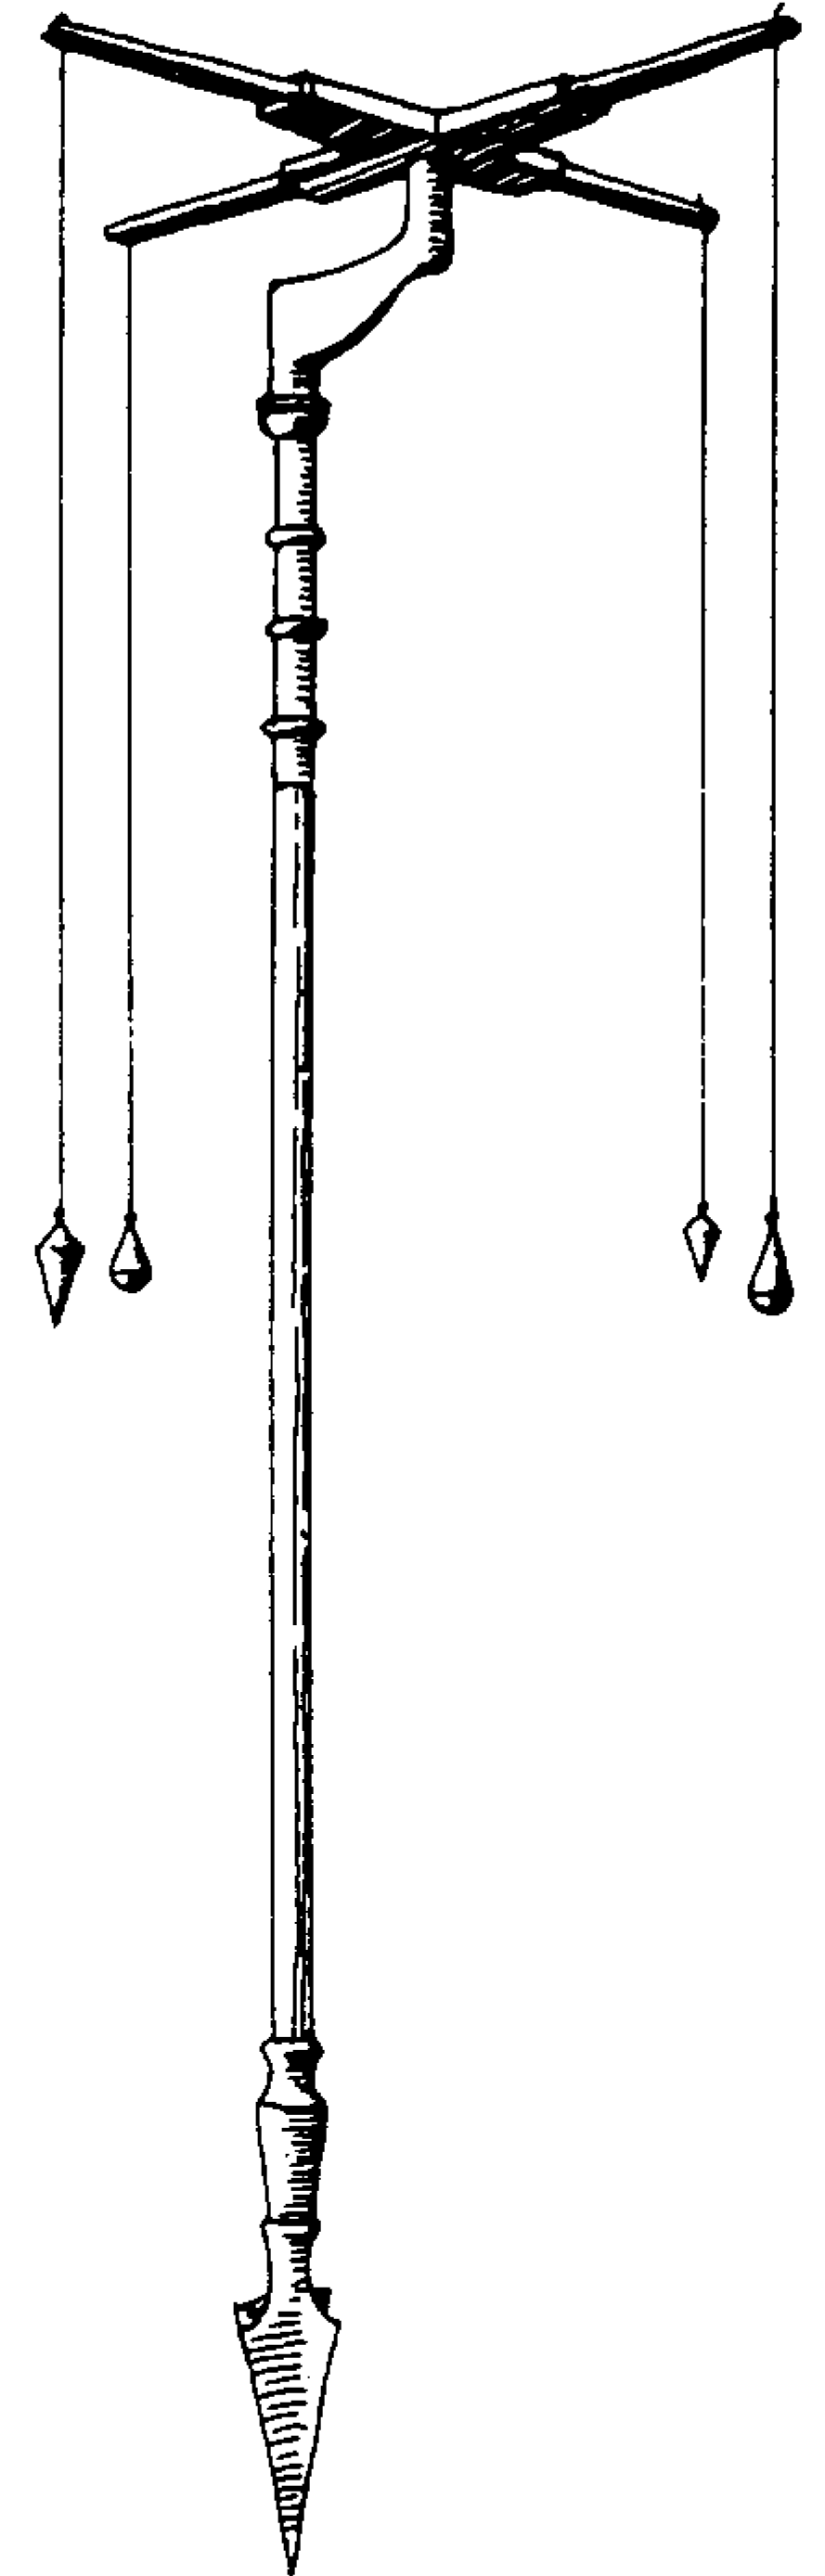
\includegraphics[height=0.8\linewidth]{2a}
		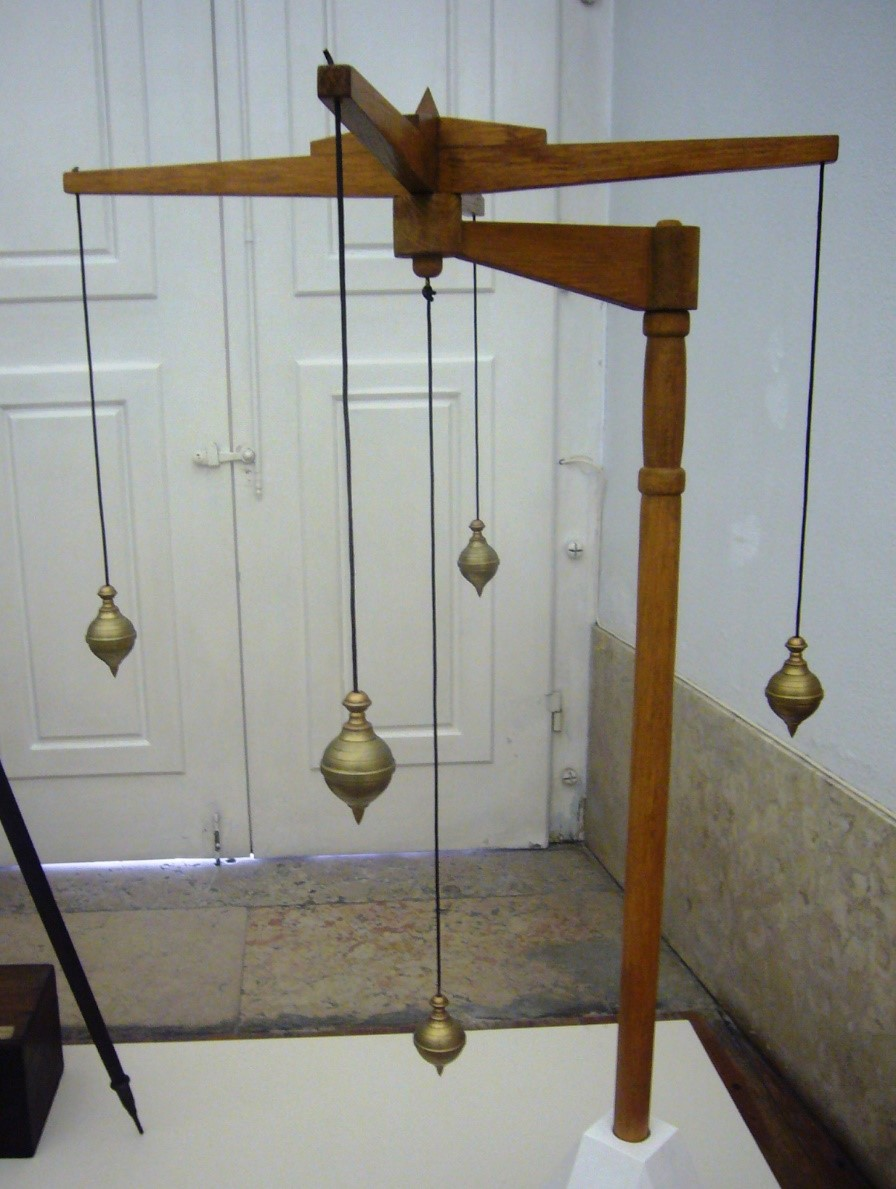
\includegraphics[height=0.8\linewidth]{2b}
		\caption{\small\textit{\color{toanhocdoisong}Hình $2$. Sơ đồ cấu tạo của groma (trái) và một phiên bản phục dựng (phải).}}
		\vspace*{-10pt}
	\end{figure}
	Việc sử dụng \textit{groma} để xác định góc vuông tương đối đơn giản. Thân chính được cắm sao cho hai dây dọi của một nhánh chữ thập  thẳng hàng với các cọc đã được cắm sẵn. Sau đó người ta cắm thêm các cọc mới gióng hàng với hai dây dọi của nhánh chữ thập còn lại để xác định phương vuông góc.
	\begin{figure}[H]
		\vspace*{-5pt}
		\centering
		\captionsetup{labelformat= empty, justification=centering}
		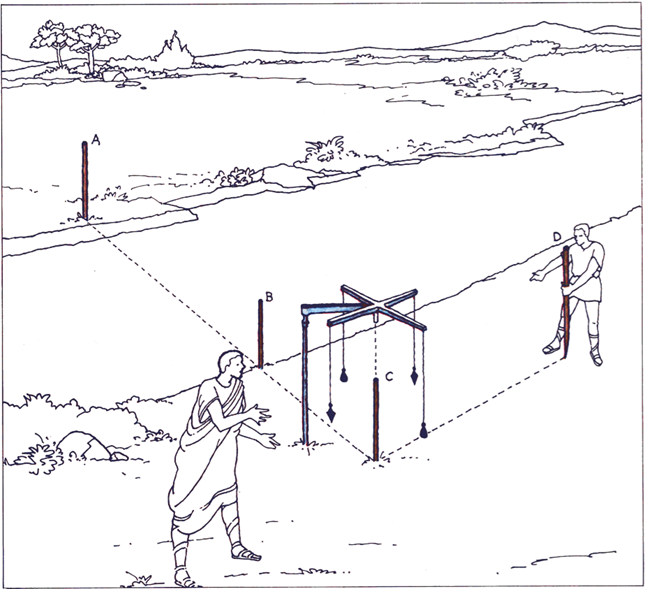
\includegraphics[width= 1\linewidth]{3}
		\caption{\small\textit{\color{toanhocdoisong}Hình $3$. Minh họa cách sử dụng groma để xác định phương vuông góc với một phương cho trước.}}
		\vspace*{-10pt}
	\end{figure}
	Về mặt lịch sử, người Ai Cập cổ đại cũng đã có một thiết bị trắc địa gần giống với \textit{groma}. Một số giả thuyết cho rằng \textit{groma} được du nhập vào xã hội La Mã từ người Etruria, những người sống ở khu vực phía bắc của nước Ý trước khi bị người La Mã sáp nhập, kèm theo đó là các nghi thức mang màu sắc tôn giáo khi sử dụng công cụ này. Do việc đo đạc xác định biên giới các công trình còn có ý nghĩa về mặt tâm linh (giống với ``động thổ" của nước ta) nên trong giai đoạn ban đầu của đế quốc La Mã, những người làm trắc địa có vai trò giống với các giáo sỹ hơn là nhân viên kỹ thuật và \textit{groma} là một biểu tượng nghi lễ gắn liền với công việc này. Dần dần, trắc địa trở thành nghề nghiệp mang tính dân sự và mất đi màu sắc huyền bí của nó.
	\vskip 0.1cm
	Bản thân \textit{groma} cũng có nhiều vấn đề về mặt kỹ thuật. Nó không thể sử dụng được khi có gió, ngay cả với gió nhẹ, do các dây dọi không còn thẳng đứng nữa. Nhà toán học Heron ở Alexandria cũng đã nhắc đến việc này. Ông đề xuất thêm các lá chắn gió cho các dây dọi nhưng cũng nhận định rằng việc này sẽ làm cho quá trình gióng hàng khó khăn hơn nhiều. Mặt khác, \textit{groma} cũng cho độ chính xác không cao. Với khoảng cách $100$ m, độ lệch của việc gióng hàng so với đường thẳng cần tìm có thể lên tới $1$ m. Một số tác giả như Jean--Pierre Adam cho rằng các bước gióng hàng liên tiếp sử dụng \textit{groma} sẽ triệt tiêu bớt sai số do ở mỗi bước do kết quả đo sẽ lệch sang trái hoặc phải một cách ngẫu nhiên. Trong khi đó, một số nhà nghiên cứu khác lại cho rằng \textit{groma} chỉ mang tính biểu tượng còn các công cụ chính của người làm trắc địa La Mã là những thiết bị chính xác hơn.
	\begin{figure}[H]
		\vspace*{-5pt}
		\centering
		\captionsetup{labelformat= empty, justification=centering}
		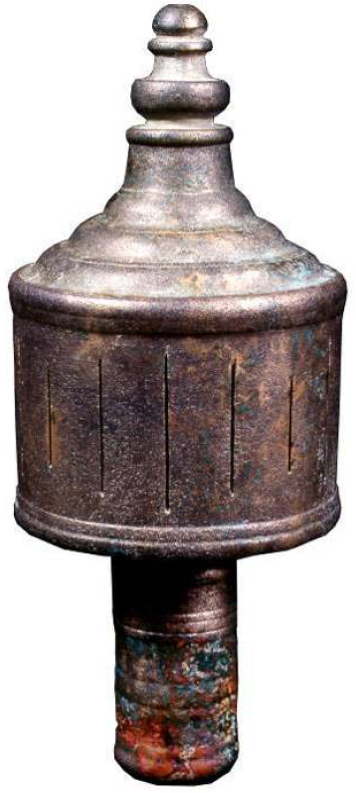
\includegraphics[width= 0.4\linewidth]{4}
		\caption{\small\textit{\color{toanhocdoisong}Hình $4$. Đầu ngắm từ thời La Mã được khai quật ở Pháp.}}
		\vspace*{-10pt}
	\end{figure}
	Năm $1997$, cuộc khai quật một di chỉ La Mã ở Pháp phát hiện một đầu ngắm hình trụ với các khe cách nhau $1/16$ đường tròn. Trước đó, người ta cũng đã phát hiện được ở Đức một dụng cụ có khe ngắm tương tự dạng bát giác (hiện vật này đã bị mất trong chiến tranh thế giới thứ hai). Điều đáng chú ý là đầu ngắm dạng này có thể cho phép xác định phương vuông góc hoặc các góc $1/4$, $1/8$ hay $1/16$  đường tròn với độ chính xác cao hơn nhiều so với \textit{groma}. Sau thời La Mã, chúng chỉ xuất hiện lại và phổ biến ở châu Âu vào thế kỷ $16$. Vì sao dụng cụ này không được nhắc đến trong những tài liệu trắc địa La Mã còn sót lại vẫn là một vấn đề hiện chưa được giải đáp.
	\vskip 0.1cm
	Một thiết bị đáng chú ý khác là \textit{dioptra}, một công cụ có nguồn gốc từ Hy Lạp. Hiện tại chỉ còn những mô tả bằng lời nên người ta không biết chính xác nó trông như thế nào. \textit{Dioptra} xuất hiện trong các phép đo thiên văn của cả Hipparchus lẫn Heron. Phiên bản của Heron có lẽ phức tạp hơn so với các phiên bản khác. Bản thân Heron cũng có một cuốn sách chuyên về trắc địa sử dụng \textit{dioptra}.
	\begin{figure}[H]
		\vspace*{-10pt}
		\centering
		\captionsetup{labelformat= empty, justification=centering}
		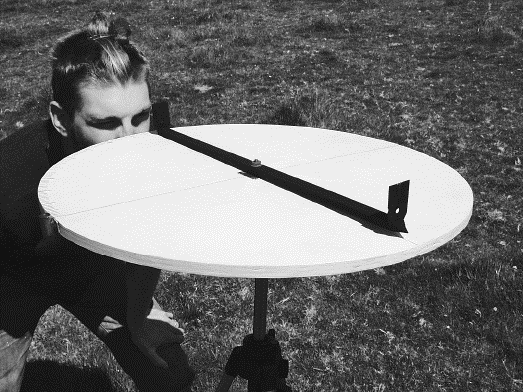
\includegraphics[height= 0.4\linewidth]{5a}
		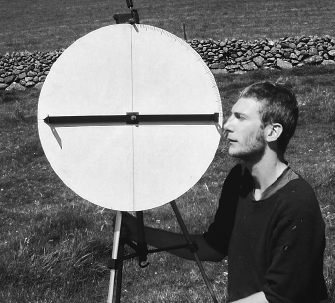
\includegraphics[height= 0.4\linewidth]{5b}
		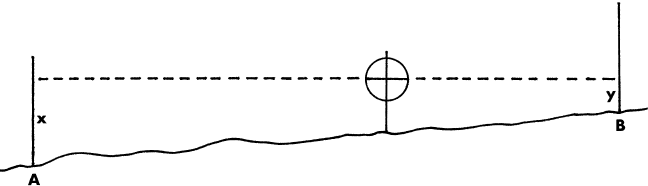
\includegraphics[width= 1\linewidth]{5c}
		\caption{\small\textit{\color{toanhocdoisong}Hình $5$. Trên: Dioptra trong mặt phẳng nằm ngang và mặt phẳng thẳng đứng. Dưới: Dùng dioptra xác định phương nằm ngang, qua đó đo được chênh lệch độ cao giữa hai điểm $A$ và $B$.}}
		\vspace*{-10pt}
	\end{figure}
	Về cơ bản, \textit{dioptra} gồm một thước ngắm trên một đĩa (gỗ hoặc kim loại). Thước ngắm có lỗ tròn hoặc khe hẹp giúp tăng độ chính xác so với chỉ ngắm bằng mắt thường qua các đầu cọc. Vạch trên đĩa vuông góc với thước cho phép xác định phương vuông góc. \textit{Dioptra} có thể được sử dụng trong mặt phẳng ngang cũng như trong mặt phẳng thẳng đứng vuông góc với mặt đất.
	\vskip 0.1cm
	Những tài liệu còn sót lại của Julius Africanus, một tác giả La Mã ở Jerusalem ở thế kỷ $3$, và một tác giả khuyết danh vào thế kỷ $10$ ở Byzantine (hậu duệ của đế quốc Đông La Mã) ghi chép về việc sử dụng \textit{dioptra} để đo khoảng cách và chiều cao. Đặc biệt, Julius Africanus mô tả cách sử dụng dioptra trong quân sự để đo chiều cao của tường thành địch. Tuy vậy, những ứng dụng này của \textit{dioptra} lại không xuất hiện trong các ghi chép có nguồn gốc ở phía Tây của đế quốc La Mã. Đây là một vấn đề hiện nay vẫn chưa thể giải thích rõ ràng. Một nguyên nhân có thể là do nguồn gốc Hy Lạp của \textit{dioptra} không được tiếp nhận tích cực ở nửa Tây của La Mã trong khi ở phía Đông, ảnh hưởng của văn minh Hy Lạp mạnh hơn (sau khi Đông La Mã trở thành Byzantine, tiếng Hy Lạp thay thế tiếng Latin thành ngôn ngữ chính thức).
	\vskip 0.1cm
	Nghiên cứu khảo cổ cũng cho thấy đồng hồ mặt trời xuất hiện trong bộ thiết bị của một nhà trắc địa La Mã cổ đại. Nó cho phép người ta xác định phương hướng vào ban ngày. Vào ban đêm, các chòm sao được dùng làm công cụ định hướng. Trong di tích nơi ở của một người làm trắc địa ở di chỉ Pompeii, có một ngôi nhà mà  sàn của nó được khảm trang trí câu chuyện về Orion, nhân vật thần thoại sau khi chết trở thành một chòm sao trên bầu trời. Chòm sao này có tác dụng quan trọng dùng để định vị các chòm sao khác. Không những cần các kỹ năng đo đạc trên mặt đất, người làm trắc địa thời La Mã còn phải có hiểu biết về bầu trời nữa!
	\begin{figure}[H]
		\vspace*{-5pt}
		\centering
		\captionsetup{labelformat= empty, justification=centering}
		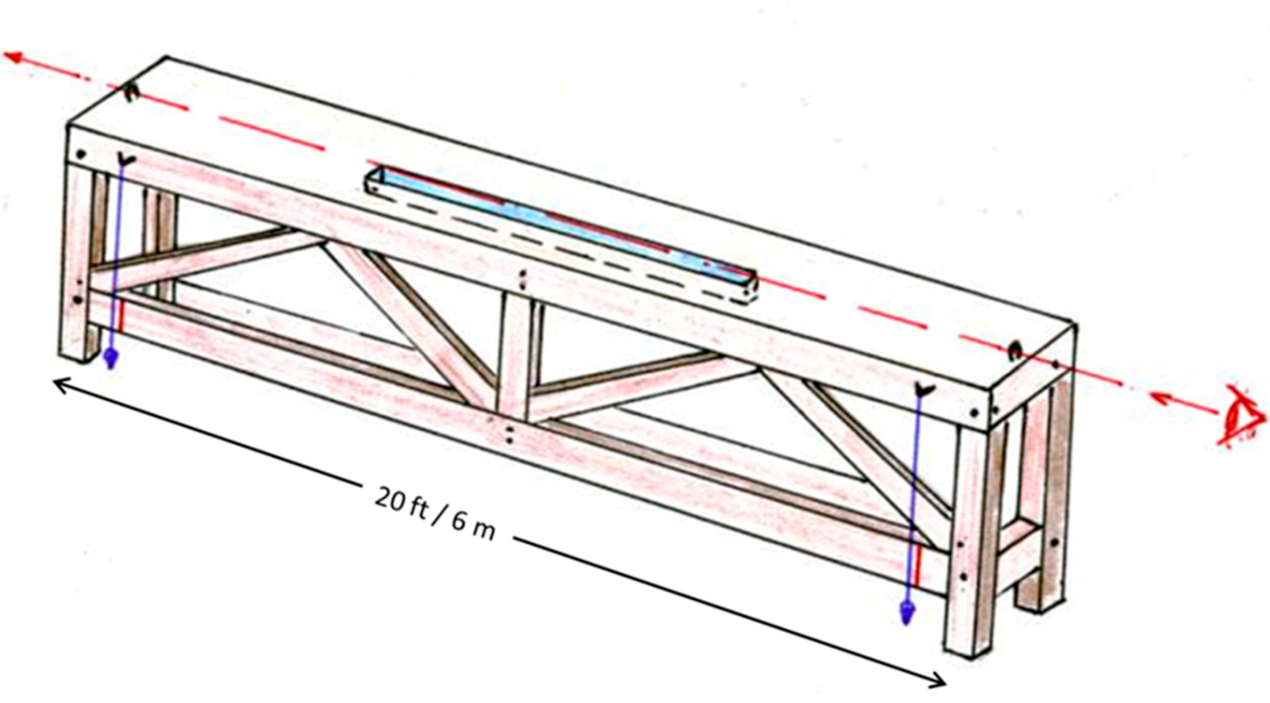
\includegraphics[width= 0.85\linewidth]{6a}
		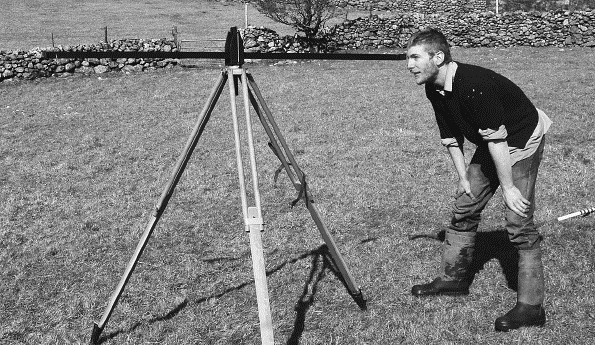
\includegraphics[width= 0.85\linewidth]{6}
		\caption{\small\textit{\color{toanhocdoisong}Hình $6$. Trên: Mô hình phục dựng lại chorobates. Dưới: Libra có cấu tạo là một thước ngắm dạng đòn cân dài có giá đỡ.}}
		\vspace*{-10pt}
	\end{figure}
	Một vấn đề trắc địa quan trọng khác là việc xác định phương nằm ngang. Đây là một yêu cầu thiết yếu khi người La Mã xây dựng các hệ thống dẫn nước dài nhiều cây số. Nhiều tài liệu hiện nay cho rằng người ta đã sử dụng thiết bị mang tên \textit{chorobates} có dạng một ghế băng dài với một máng khoét ở giữa có đổ nước. Khi mặt ghế hoàn toàn nằm ngang, mực nước sẽ ở đều cả hai bên máng. Tuy nhiên, về mặt kỹ thuật, độ chính xác của nó không cao và các thiết bị chính xác hơn nhiều như \textit{dioptra} và \textit{libra} có thể đã được sử dụng (Hình $6$). 
	\vskip 0.1cm
	Về mặt đo khoảng cách, ngoài dây thừng và gậy, người La Mã có một thiết bị khá thú vị là \textit{hodometer} có nguồn gốc Hy Lạp. Khi người sử dụng đẩy xe, trục bánh xe sẽ kéo theo các bánh răng bên trong xe chuyển động. Các bánh răng được tính toán sao cho khi xe đi được một dặm La Mã, một hòn sỏi sẽ chui qua lỗ ở trên xuống phía dưới và ta chỉ cần đếm số lượng hòn sỏi để biết đã đi được bao xa. Tuy khá phức tạp về mặt cơ khí, \textit{hodometer} không có độ chính xác cao do quá trình di chuyển khi đẩy xe giữa hai điểm trong thực tế thường gấp khúc chứ không phải đường thẳng.
	\begin{figure}[H]
		\vspace*{-5pt}
		\centering
		\captionsetup{labelformat= empty, justification=centering}
		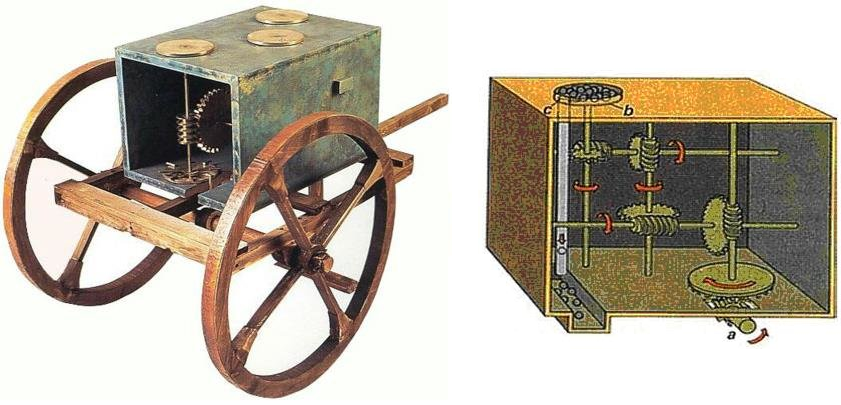
\includegraphics[width= 1\linewidth]{7}
		\caption{\small\textit{\color{toanhocdoisong}Hình $7$. Hodometer.}}
		\vspace*{-10pt}
	\end{figure}
	\textbf{\color{toanhocdoisong}Bài tập}
	\vskip 0.1cm
	Trong các bài tập trắc địa dưới đây, phương vuông góc có thể được xác định bằng \textit{groma} hoặc \textit{dioptra}.
	\vskip 0.1cm
	$\pmb{1.}$ \textit{Tìm khoảng cách giữa điểm $A$ (ở gần) và điểm $B$ (ở xa) mà không cần đi đến $B$.} 
	\vskip 0.1cm
	Phương pháp: Cắm cọc ở $G$  thẳng hàng với $A$ và $B$. Cắm cọc ở $E$ sao cho $G E$ vuông góc với $BG$. Trên $BE$, xác định $D$ sao cho $AD$ vuông góc với $BG$. Đo các khoảng cách $AD$, $AG$, $EG$.
	\vskip 0.1cm 
	Hãy viết biểu thức của độ dài đoạn $AB$.
	\begin{figure}[H]
		\vspace*{-5pt}
		\centering
		\captionsetup{labelformat= empty, justification=centering}
		\begin{tikzpicture}[color=toanhocdoisong,scale=0.72, node font=\small]
			\draw  (0.,0.)-- (5.,0.);
			\draw  (5.,0.)-- (5.,3.);
			\draw  (5.,3.)-- (0.,0.);
			\draw  (3.,0.)-- (3.0176470588235293,1.8105882352941176);
			\draw [fill=white] (0.,0.) circle (1.5pt);
			\draw (-0.4,-0.09) node {$B$};
			\draw [fill=white] (5.,0.) circle (1.5pt);
			\draw (5.22,-0.5) node {$G$};
			\draw [fill=white] (5.,3.) circle (1.5pt);
			\draw (5.14,3.37) node {$E$};
			\draw [fill=white] (3.,0.) circle (1.5pt);
			\draw (2.96,-0.5) node {$A$};
			\draw [fill=white] (3.0176470588235293,1.8105882352941176) circle (1.5pt);
			\draw (3.03,2.32) node {$D$};
		\end{tikzpicture}
		\vspace*{-10pt}
	\end{figure}
	$\pmb{2.}$ \textit{Đo chiều cao của bức tường $AB$ mà không đến $B$.} 
	\vskip 0.1cm
	Phương pháp: Cắm \textit{dioptra} tại $G$ và gióng thước ngắm đến $A$. Giữ nguyên thước ngắm và ngắm theo chiều ngược lại để xác định điểm $E$ trên mặt đất. Đo $G E$ và $GD$ với $D$ là tâm của đĩa tròn của \textit{dioptra}. Đo $EB$ theo phương pháp ở bài $1$.
	\vskip 0.1cm 
	Hãy viết biểu thức cho độ cao $AB$.  
	\begin{figure}[H]
		\vspace*{-5pt}
		\centering
		\captionsetup{labelformat= empty, justification=centering}
		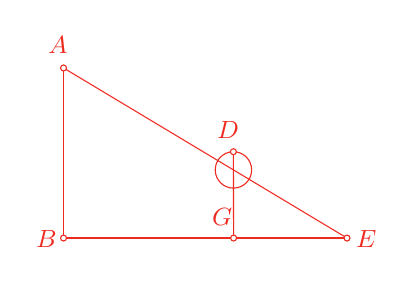
\begin{tikzpicture}[color=toanhocdoisong, scale=0.72, node font=\small]
			\draw  (0.,4.)-- (0.,1.);
			\draw  (0.,1.)-- (5.,1.);
			\draw  (5.,1.)-- (0.,4.);
			\draw  (2.9970588235294118,2.201764705882353)-- (3.,1.);
			\draw  (2.9970588235294118,2.201764705882353) circle (0.3210460842858762cm);
			\draw  (2.9970588235294118,2.201764705882353)-- (2.996273103698748,2.5228098286916585);
				\draw [fill=white] (0.,4.) circle (1.5pt);
				\draw (-0.1,4.41) node {$A$};
				\draw [fill=white] (0.,1.) circle (1.5pt);
				\draw (-0.3,0.99) node {$B$};
				\draw [fill=white] (5.,1.) circle (1.5pt);
				\draw (5.34,0.99) node {$E$};
				\draw [fill=white] (3.,1.) circle (1.5pt);
				\draw (2.8,1.38) node {$G$};
				\draw [fill=white] (2.996273103698748,2.5228098286916585) circle (1.5pt);
				\draw (2.9,2.9) node {$D$};
		\end{tikzpicture}
		\vspace*{-10pt}
	\end{figure}
	$\pmb{3.}$ $a)$ \textit{Đo khoảng cách giữa hai điểm $A$ và $B$ có thể nhìn thấy nhưng không thể đến được.}
	\vskip 0.1cm 
	Phương pháp: Sử dụng phương pháp ở bài $1$ để đo các khoảng cách $G A$ và $G B$ khi đứng ở $G$. Gióng các cọc tại $D$ và $E$ sao cho $\dfrac{GD}{G E}=\dfrac{G A}{G B}$. Đo độ dài $D E$.
	\vskip 0.1cm 
	Hãy viết biểu thức cho độ dài $AB$.
	\begin{figure}[H]
		\vspace*{-5pt}
		\centering
		\captionsetup{labelformat= empty, justification=centering}
		\begin{tikzpicture}[color=toanhocdoisong, scale=0.72, node font=\small]
			\draw  (2.,2.)-- (0.,5.);
			\draw  (-4.5,2.)-- (2.,2.);
			\draw  (-2.076923076923077,3.6153846153846154)-- (-1.,2.);
			\draw  (-4.5,2.)-- (0.,5.);
			
			\draw [fill=white] (2.,2.) circle (1.5pt);
			\draw (2.3,1.93) node {$B$};
			\draw [fill=white] (0.,5.) circle (1.5pt);
			\draw (0.14,5.37) node {$A$};
			\draw [fill=white] (-4.5,2.) circle (1.5pt);
			\draw (-4.9,1.93) node {$G$};
			\draw [fill=white] (-1.,2.) circle (1.5pt);
			\draw (-0.92,1.55) node {$E$};
			\draw [fill=white] (-2.076923076923077,3.6153846153846154) circle (1.5pt);
			\draw (-2.2,3.99) node {$D$};
		\end{tikzpicture}
		\vspace*{-10pt}
	\end{figure}
	$b)$ Hãy chứng minh $D E$ song song với $AB$ để chỉ ra rằng phương pháp trên cũng cho phép xác định phương song song với đường thẳng đi qua hai điểm ở xa.
	\vskip 0.1cm
	$\pmb{2.}$ \textbf{\color{toanhocdoisong}Trắc địa trên khoảng cách lớn}
	\vskip 0.1cm
	Trong việc xây dựng các con đường nối hai địa điểm, trừ khi có chướng ngại vật, người ta luôn hướng đến việc đi theo đường thẳng thay vì đường cong. Việc xác định đường thẳng trên thực địa là một vấn đề quan trọng mà người làm trắc địa La Mã cần phải giải quyết. Các công cụ gióng hàng nêu ở phần trên có thể giúp gióng hàng ở khoảng cách ngắn từ vài trăm mét đến vài ki--lô--mét. Với những khoảng cách lớn hơn, vấn đề bắt đầu trở nên phức tạp hơn.
	\begin{figure}[H]
		\vspace*{-5pt}
		\centering
		\captionsetup{labelformat= empty, justification=centering}
		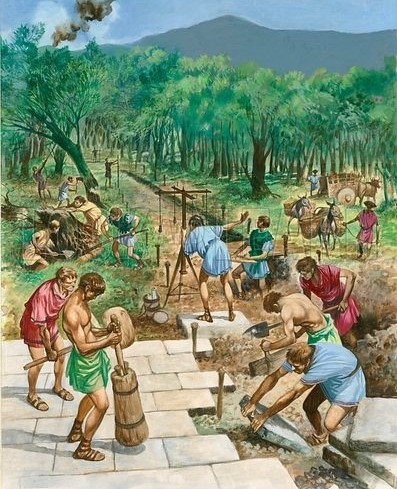
\includegraphics[height= 0.8\linewidth]{8}
		\caption{\small\textit{\color{toanhocdoisong}Hình $8$. Minh họa về xây dựng đường thời La Mã (Peter Jackson). Kỹ thuật viên ở giữa đang gióng hàng với một người cầm cọc và một cột khói ở địa điểm ở phía xa.}}
		\vspace*{-10pt}
	\end{figure}
	Nếu không thể nhìn thấy điểm kết thúc từ điểm bắt đầu con đường, người ta có thể đốt lửa tạo cột khói để tiến hành gióng hàng. Tuy nhiên, với những khoảng cách lớn hơn nữa, công việc cũng trở nên phức tạp hơn nhiều. 
	\begin{figure}[H]
		\vspace*{-5pt}
		\centering
		\captionsetup{labelformat= empty, justification=centering}
		\begin{tikzpicture}[scale=0.7, color=toanhocdoisong]
			\draw [dashed] (0,0) -- (10,0);
			\draw [fill= black] (0,0) circle (3pt);
			\draw [fill= white] (2,0.5) circle (3pt);
			\draw [fill= white] (4,-0.5) circle (3pt);
			\draw [fill= white] (6,0.5) circle (3pt);
			\draw [fill= white] (8,-0.5) circle (3pt);
			\draw [fill= black] (10,0) circle (3pt);
		\end{tikzpicture}
		\caption{\small\textit{\color{toanhocdoisong}Hình $9$. Gióng hàng bằng xấp xỉ liên tiếp. Các cọc màu trắng sẽ được di chuyển đến lúc nào tất cả chúng đều thẳng hàng với hai vị trí đầu và cuối (hai cọc màu đen).}}
		\vspace*{-10pt}
	\end{figure}
	Một giả thuyết được đưa ra là đầu tiên người ta cắm một số cọc đánh dấu xấp xỉ, mỗi cọc chỉ có thể quan sát được một cọc phía trước và một cọc phía sau. Do không xác định chính xác được đường thẳng nối điểm đầu và điểm cuối trên thực địa, các cọc sẽ được di chuyển bằng cách thử dần cho đến khi nào tất cả các cọc đều thẳng hàng (kể cả cọc cố định ở điểm đầu và điểm cuối). Phương pháp xấp xỉ liên tiếp này tuy có thể thực hiện được nhưng sẽ mất rất nhiều thời gian và công sức lao động.
	\vskip 0.1cm
	Một giả thuyết khác là các nhà trắc địa La Mã đã sử dụng cách đo khoảng cách của Heron. Chọn một phương làm phương cơ sở (ví dụ phương Đông Tây). Sau đó ta chỉ di chuyển theo phương này hoặc phương vuông góc với nó. Đến mỗi điểm đánh dấu (ví dụ ngọn đồi), người ta ghi lại tổng độ dài đã đi theo mỗi phương. Từ đó, một bản đồ giống với lưới tọa độ có thể được vẽ ra. Các vị trí trên đường đi sẽ được thiết lập theo độ lệch của nó so với đường gấp khúc nối các điểm đánh dấu.
	\begin{figure}[H]
		\vspace*{-5pt}
		\centering
		\captionsetup{labelformat= empty, justification=centering}
		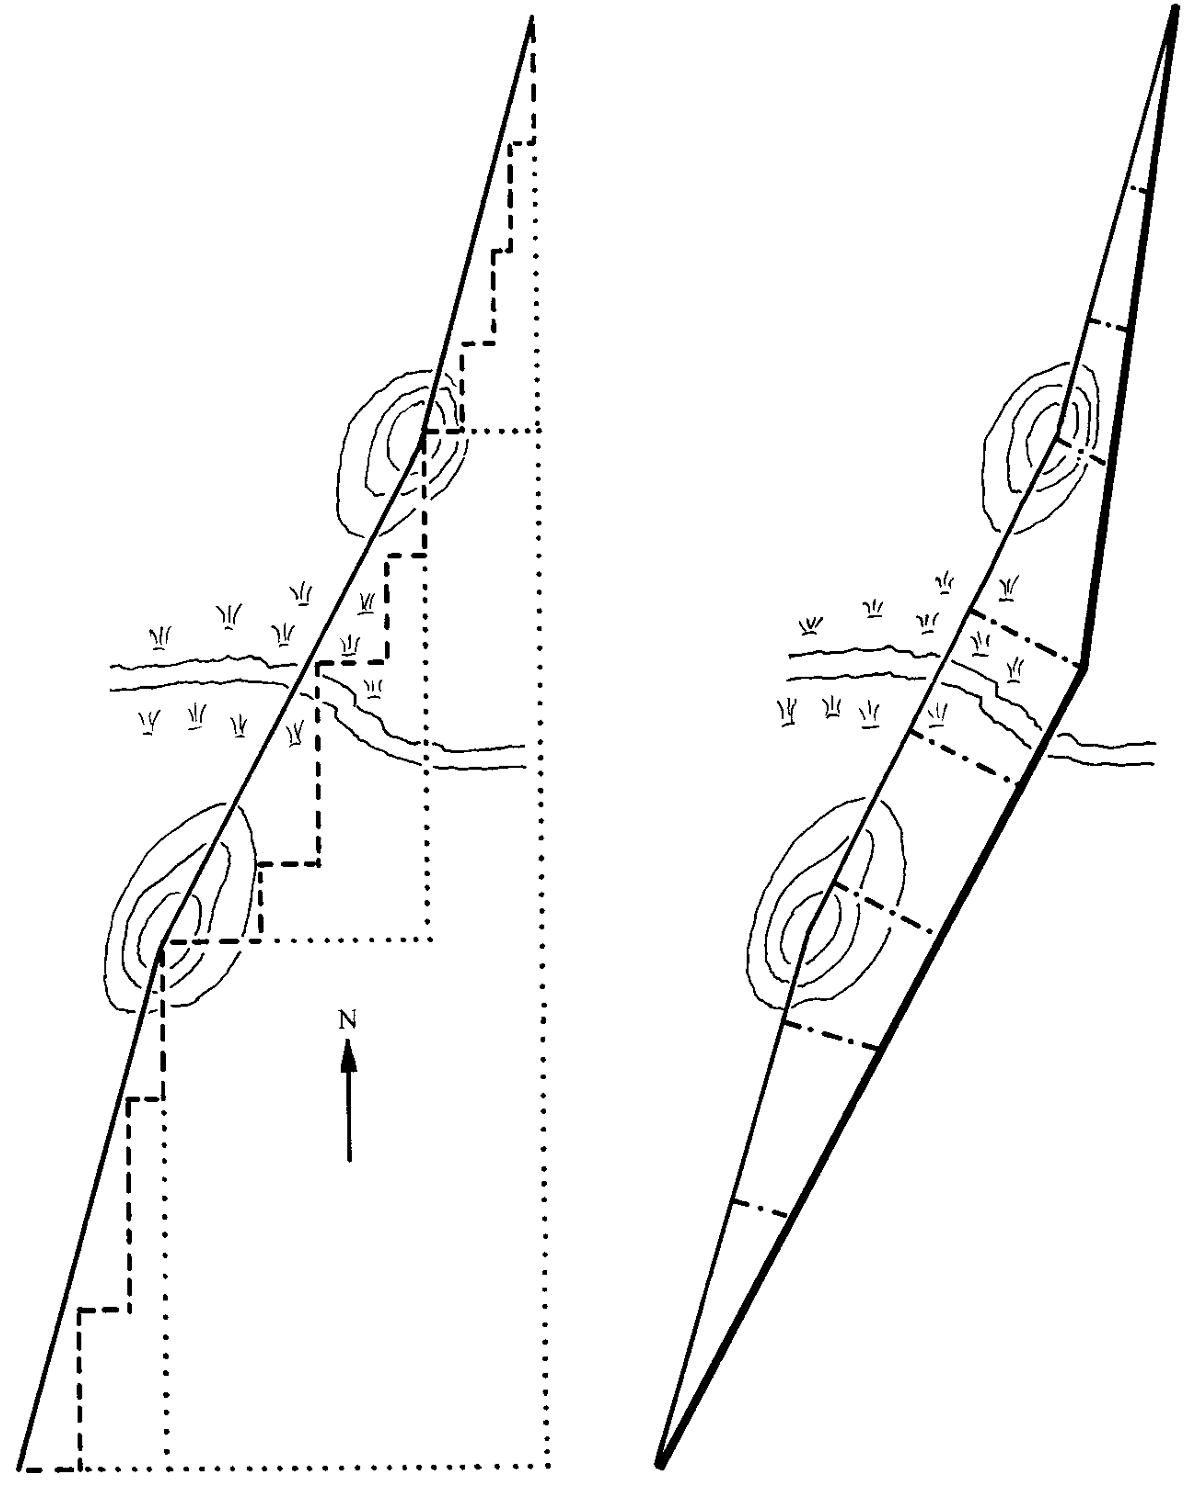
\includegraphics[height= 0.7\linewidth]{10}
		\caption{\small\textit{\color{toanhocdoisong}Hình $10$. Xác định vị trí bằng cách di chuyển theo hai phương vuông góc.}}
		\vspace*{-10pt}
	\end{figure}
	Trong một phiên bản khác của phương pháp này, việc trắc địa sẽ không có thao tác vẽ bản đồ mà được hoàn toàn tiến hành trên thực địa. Ứng với mỗi điểm đánh dấu, người ta đo khoảng cách đến điểm đánh dấu trước nó bằng các phương pháp đo trắc địa. Góc của đường nối cũng được xác định bằng góc so với phương Bắc – Nam. Góc ở giai đoạn lịch sử này không biểu diễn bằng độ mà được biểu diễn bằng tỷ lệ giữa hai cạnh góc vuông -- tức là $\tan$ của góc. Khoảng cách và góc giữa điểm đầu và điểm cuối có thể được xác định bằng cách tính các cạnh của tam giác vuông theo định lý Pythagoras và tam giác đồng dạng. Nhờ đó, có thể tiến hành gióng hàng để xác định đường thẳng nối hai điểm đã cho.
	\begin{figure}[H]
		\vspace*{-5pt}
		\centering
		\captionsetup{labelformat= empty, justification=centering}
		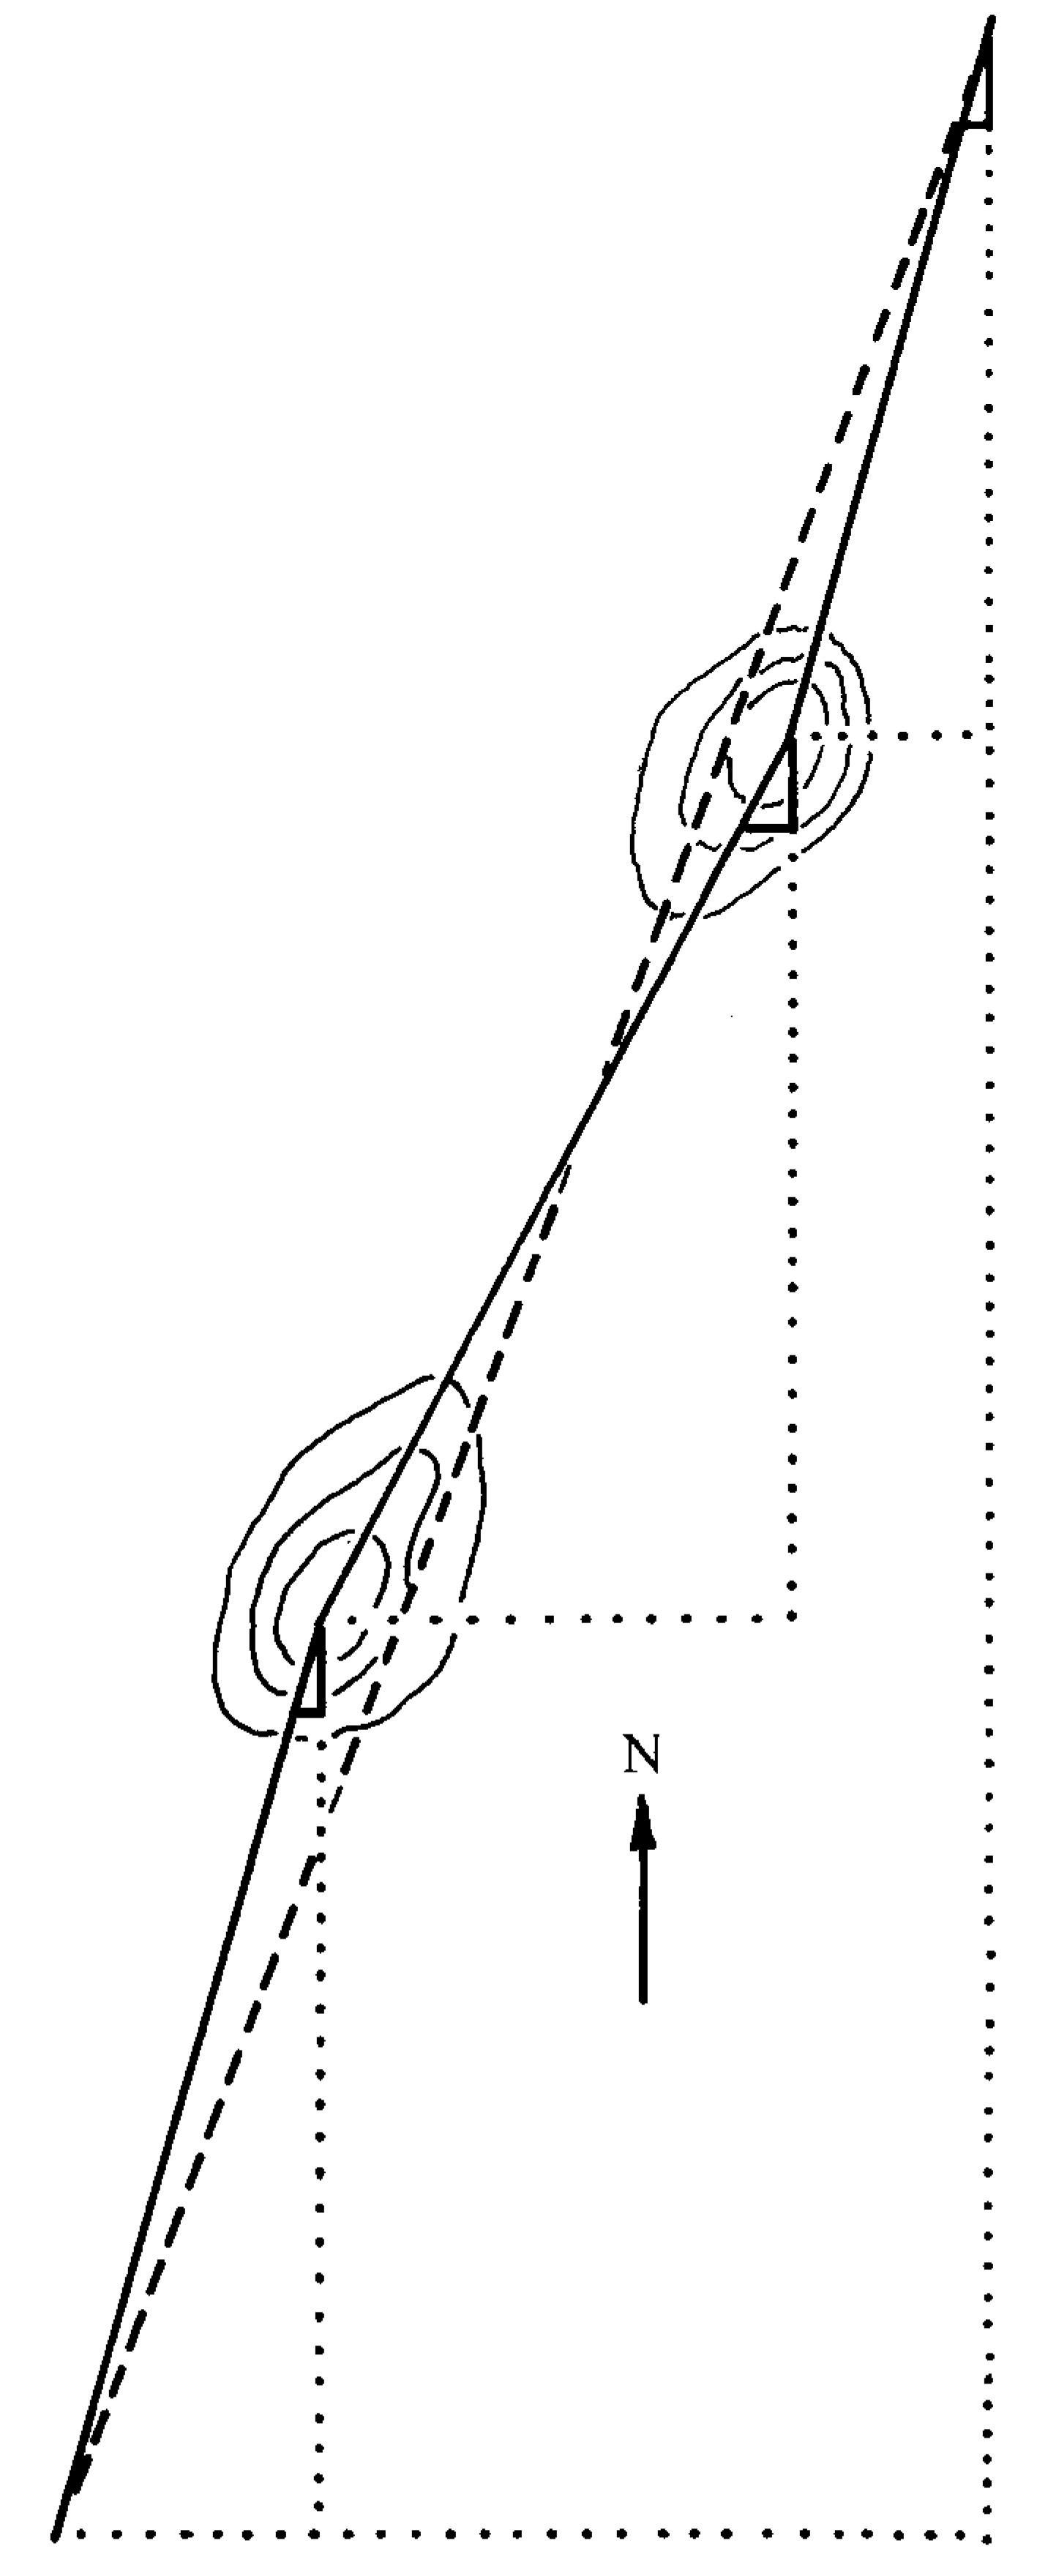
\includegraphics[height= 0.7\linewidth]{11}
		\caption{\small\textit{\color{toanhocdoisong}Hình $11$. Xác định vị trí theo khoảng cách và góc.}}
		\vspace*{-10pt}
	\end{figure}
	Một giả thuyết khác được nhà nghiên cứu M. Lewis đưa ra là việc gióng hàng trên khoảng cách lớn bằng dựng hình. Theo đó, người ta tiến hành gióng hàng theo một phương $AX$ mang tính ước lượng và xác định xem $B$ nằm ở nửa mặt phẳng nào so với $AX$, sau đó tiến hành gióng hàng theo hai phương $AY$ và $AZ$ sao cho $B$ nằm trong góc tạo bởi hai tia này. Khi đến đủ gần để chắc chắn rằng $B$ đúng là như vậy, các đường song song với $AY$ và $AZ$ được gióng từ $B$ (bằng cách sử dụng góc tạo với phương Bắc – Nam theo dạng tỷ lệ hai cạnh góc vuông) để tạo hình bình hành $ACBD$. Sau khi đo khoảng cách $CD$, trung điểm $E$ của đoạn thẳng này có thể được xác định. Điểm $E$ đồng thời cũng là trung điểm của $AB$. Các trung điểm của $AE$ và $EB$ có thể được tìm ra một cách tương tự. Quá trình xác định các trung điểm được lặp lại cho đến khi tất cả vị trí có thể được gióng hàng bằng các cọc liên tiếp sử dụng \textit{groma} hoặc \textit{dioptra}. 
	\vskip 0.1cm
	Một điểm đáng chú ý là một số con đường La Mã không được xây dựng hoàn toàn từ số không mà có mục đích nối các trung tâm dân cư đã có sẵn từ trước khi người La Mã đặt chân đến. Những con đường nối các địa điểm này dần hình thành theo lịch sử do hoạt động giao thông của con người cũng như việc chăn thả gia súc. Các đàn gia súc thường đi theo đường thẳng giữa các điểm có nhiều cỏ và nguồn nước -- đây cũng là các điểm mà dân cư thường tụ tập. Do đó công việc trắc địa có những lúc được tiến hành một cách dễ dàng hơn dựa trên việc nắn thẳng lại các tuyến đường có sẵn.
		\begin{figure}[H]
		\vspace*{-10pt}
		\centering
		\captionsetup{labelformat= empty, justification=centering}
		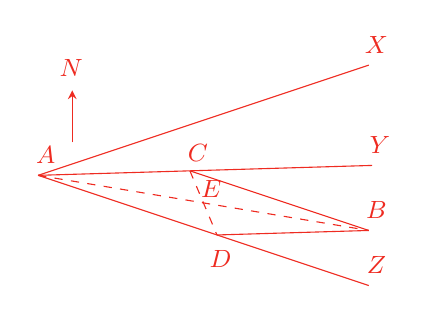
\begin{tikzpicture}[toanhocdoisong, scale=0.7, node font=\small]
			\draw  (-4.,2.)-- (2.06,2.18);
			\draw  (2.,4.)-- (-4.,2.);
			\draw  (-4.,2.)-- (2.,0.);
			\draw[dashed]  (-4.,2.)-- (2.,1.);
			\draw[-stealth]  (-3.38,2.6)-- (-3.38,3.54);
			\draw  (-1.245454545454544,2.0818181818181816)-- (2.,1.);
			\draw  (2.,1.)-- (-0.7545454545454544,0.9181818181818181);
			\draw[dashed]  (-1.245454545454544,2.0818181818181816)-- (-0.7545454545454544,0.9181818181818181);
			%			\draw [fill=white] (-4.,2.) circle (1.5pt);
			\draw (-3.86,2.37) node {$A$};
			%			\draw [fill=white] (2.06,2.18) circle (1.5pt);
			\draw (2.2,2.55) node {$Y$};
			%			\draw [fill=white] (2.,4.) circle (1.5pt);
			\draw (2.14,4.37) node {$X$};
			%			\draw [fill=white] (2.,0.) circle (1.5pt);
			\draw (2.14,0.37) node {$Z$};
			%			\draw [fill=white] (2.,1.) circle (1.5pt);
			\draw (2.14,1.37) node {$B$};
			%			\draw [fill=white] (-1.,1.5) circle (1.5pt);
			\draw (-0.86,1.75) node {$E$};
			%			\draw [fill=white] (-1.245454545454544,2.0818181818181816) circle (1.5pt);
			\draw (-1.1,2.41) node {$C$};
			%			\draw [fill=white] (-0.7545454545454544,0.9181818181818181) circle (1.5pt);
			\draw (-0.69,0.49) node {$D$};
			%			\draw [fill=white] (-3.38,3.54) circle (1.5pt);
			\draw (-3.4,3.95) node {$N$};
			%			\draw[color=black] (-1.24,1.55) node {$p$};
		\end{tikzpicture}
		\caption{\small\textit{\color{toanhocdoisong}Hình $12$. Trắc địa bằng dựng hình.}}
		\vspace*{-10pt}
	\end{figure}
	Có thể nói, phương pháp gióng hàng trên khoảng cách lớn mà người La Mã đã sử dụng vẫn là một vấn đề mở với các hướng nghiên cứu khác nhau và khó có thể kết luận được một cách dễ dàng với lượng chứng cứ ít ỏi còn lại.
	\vskip 0.1cm
	$\pmb{3.}$ \textbf{\color{toanhocdoisong}Vai trò của trắc địa trong kinh tế xã hội La Mã}
	\begin{figure}[H]
		\vspace*{-5pt}
		\centering
		\captionsetup{labelformat= empty, justification=centering}
		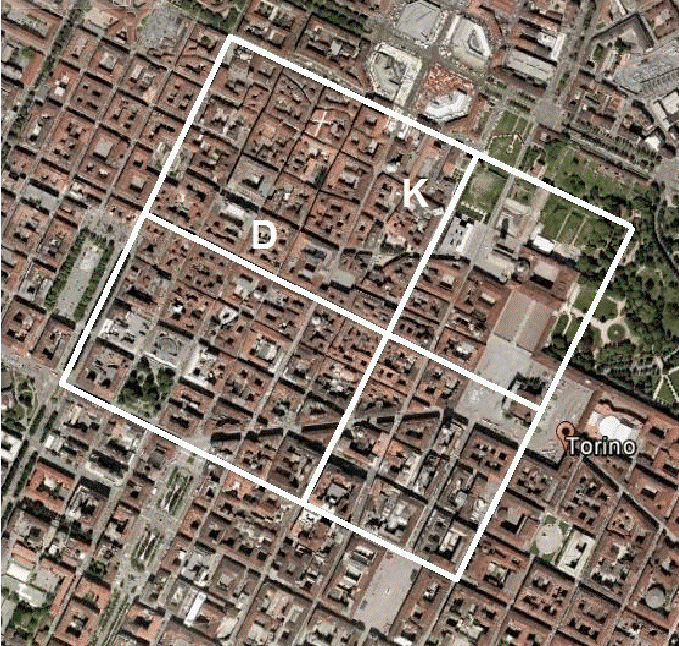
\includegraphics[height= 0.7\linewidth]{13}
		\caption{\small\textit{\color{toanhocdoisong}Hình $13$. Lưới ô vuông của một di tích La Mã.}}
		\vspace*{-10pt}
	\end{figure}
	Trắc địa có dấu ấn quan trọng trong việc quy hoạch các khu vực đô thị cũng như đất nông nghiệp ở La Mã. Các khu vực này sẽ được chia theo các lưới ô vuông dọc theo các trục đường chính trước khi xây dựng. Những người làm trắc địa không chỉ tiến hành đo đạc mà còn phải có hiểu biết về pháp luật để tiến hành giải quyết các tranh chấp khiếu kiện về đất đai.
	\begin{figure}[H]
		\vspace*{-5pt}
		\centering
		\captionsetup{labelformat= empty, justification=centering}
		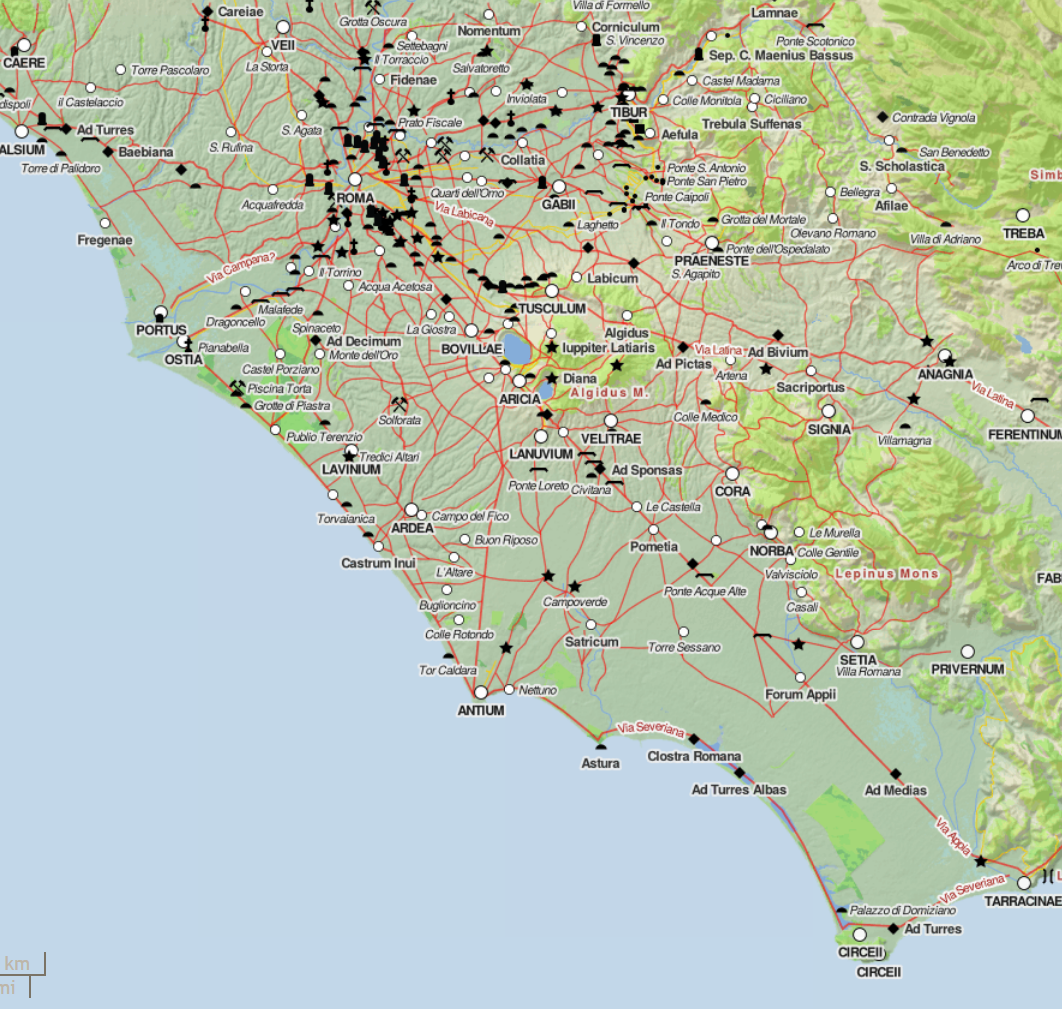
\includegraphics[height= 0.65\linewidth]{14}
		\caption{\small\textit{\color{toanhocdoisong}Hình $14$. Hệ thống đường giao thông xung quanh Rome thời La Mã cổ đại.}}
		\vspace*{-10pt}
	\end{figure}
	Hệ thống đường giao thông La Mã cũng mang đậm dấu ấn của những nhà trắc địa. Mạng lưới đường bộ trải khắp đế quốc được thiết kế với mức độ thẳng nhất mà địa hình cho phép, giúp đảm bảo tốc độ vận chuyển nhanh chóng nhất cho các hoạt động kinh tế cũng như quân sự của một đế quốc khổng lồ. Nhiều đoạn đường trong hệ thống này có độ dài thẳng tắp từ vài chục đến hàng trăm ki--lô--mét.
	
	\begin{figure}[H]
		\vspace*{-5pt}
		\centering
		\captionsetup{labelformat= empty, justification=centering}
		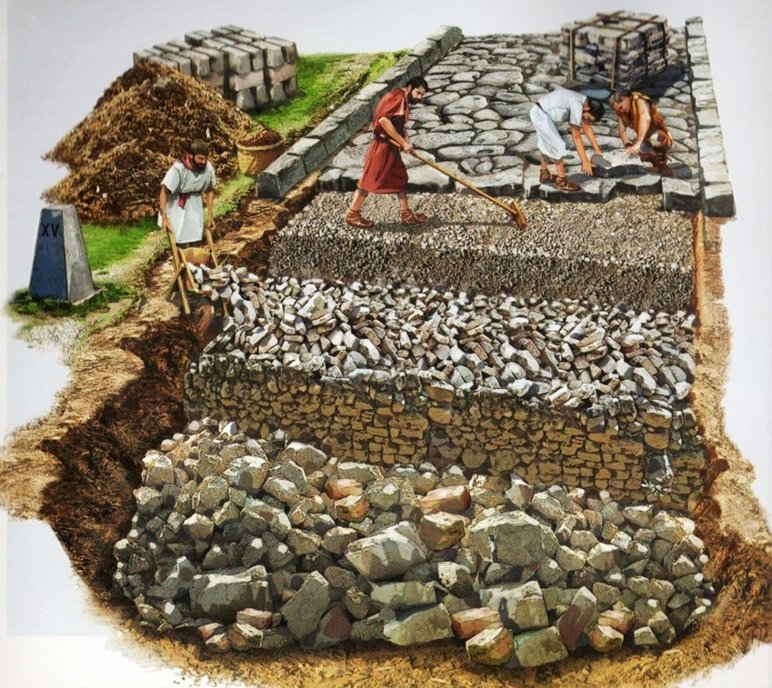
\includegraphics[height= 0.36\linewidth]{15a}
		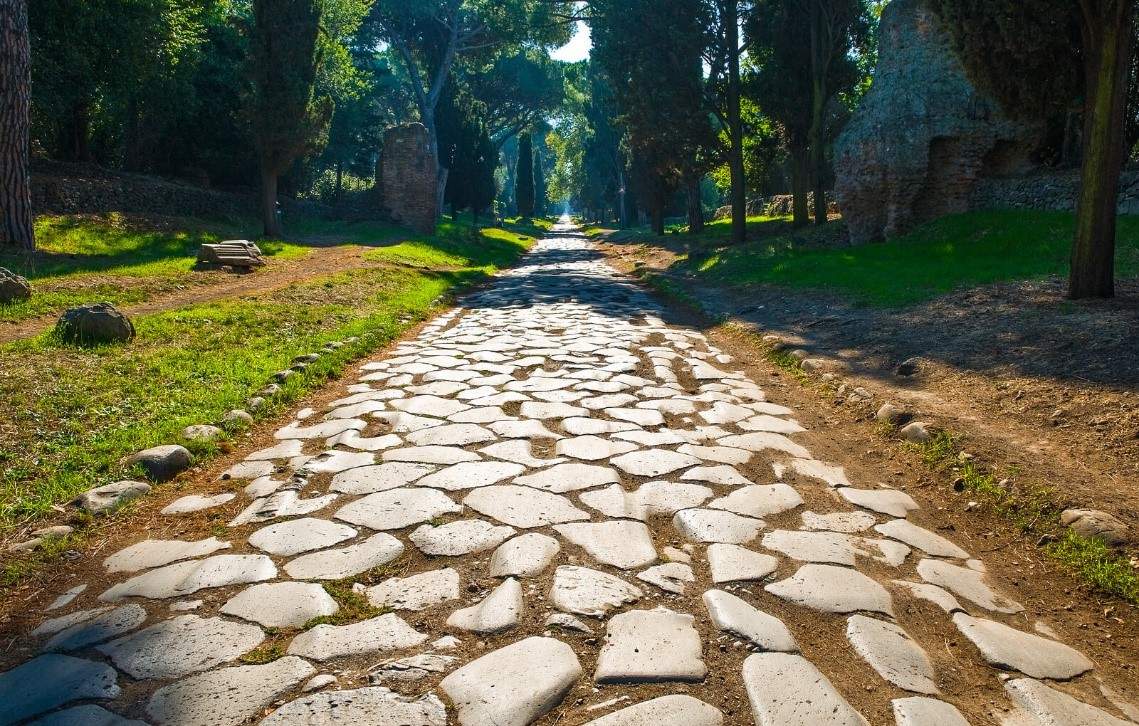
\includegraphics[height= 0.36\linewidth]{15b}
		\caption{\small\textit{\color{toanhocdoisong}Hình $15$. Trái: Đường bộ thời La Mã được xây dựng công phu với nhiều lớp vật liệu khác nhau. Phải: Một con đường thời La Mã vẫn tồn tại đến ngày nay.}}
		\vspace*{-10pt}
	\end{figure}
	Các con đường thời La Mã được xây dựng một cách công phu với nhiều lớp vật liệu khác nhau đảm bảo tính bền chắc cũng như thoát nước tốt. Nhiều đoạn vẫn còn tồn tại hàng nghìn năm cho đến ngày nay. Dọc theo các con đường là những cột mốc đánh dấu khoảng cách tính từ cột mốc số không, được đặt tại Rome -- đầu não của toàn bộ đế quốc. Đây cũng là nguồn gốc của câu nói ``Mọi con đường đều dẫn đến Rome".
	\vskip 0.1cm
	Một thành tựu đáng chú ý khác của trắc địa thời La Mã là việc xây dựng các hệ thống đường ống dẫn nước (\textit{aqueduct}). Để cung cấp nước sinh hoạt cho khu vực đô thị, người ta phải dẫn nguồn nước từ các vị trí cao như suối hay hồ trên núi theo hệ thống đường dẫn có thể lên đến hàng chục ki--lô--mét. Do chưa biết đến hiện tượng bình thông nhau, toàn bộ hệ thống ống dẫn được xây dựng với độ dốc hướng xuống. Trên những quãng đường xa như vậy, độ dốc này phải rất nhỏ, trung bình khoảng một trên vài nghìn, ở một số đoạn độ dốc chỉ là $1/20000$. Có những đoạn phải được đào theo những đường hầm xuyên núi. Những hệ thống dẫn nước này cho thấy độ chính xác cao trong việc tiến hành trắc địa và đo đạc khi xây dựng. Đồng thời, chúng cũng là biểu tượng cho sự thịnh vượng và phồn vinh của đế quốc La Mã.
	\begin{figure}[H]
		\vspace*{-5pt}
		\centering
		\captionsetup{labelformat= empty, justification=centering}
		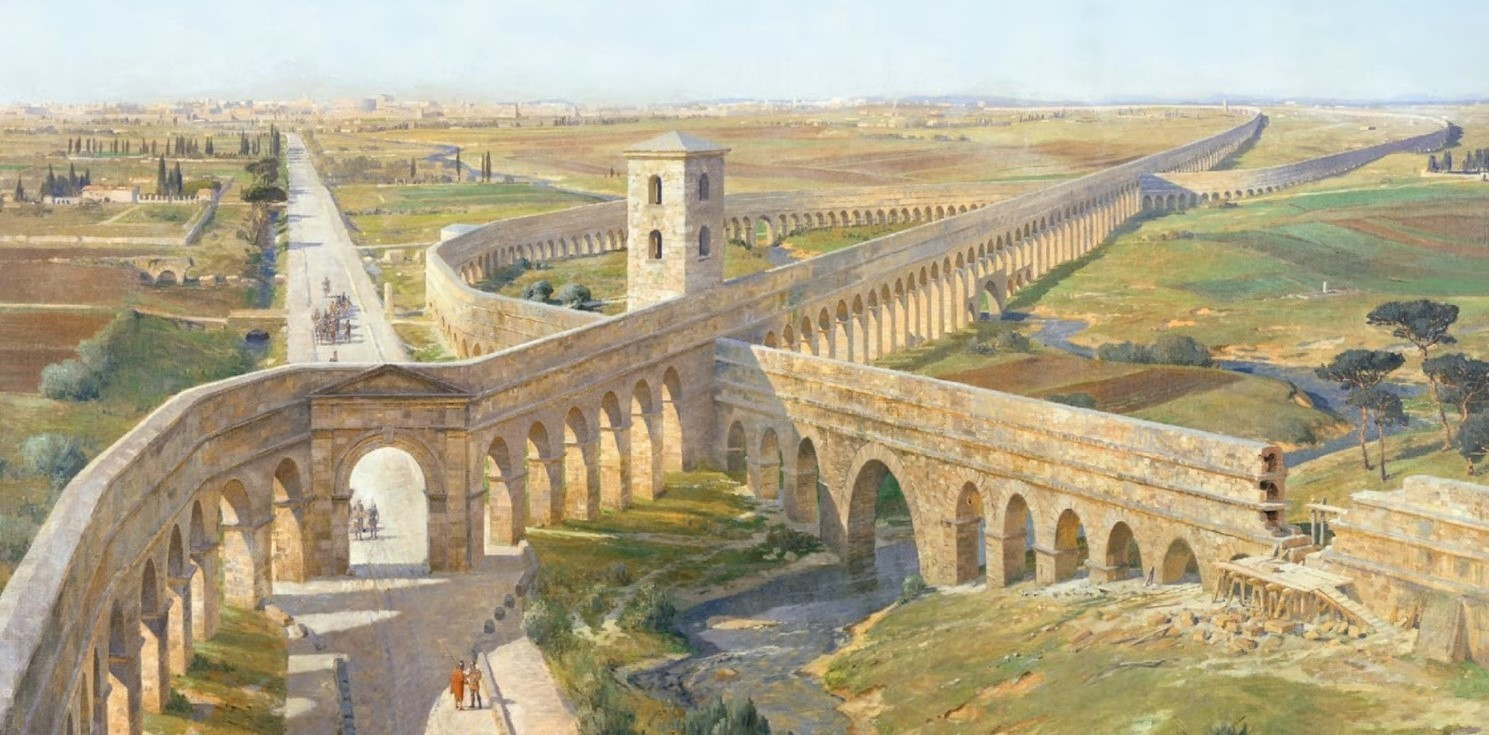
\includegraphics[width= 1\linewidth]{16}
		\caption{\small\textit{\color{toanhocdoisong}Hình $16$. Hệ thống dẫn nước gần thành Rome}}
		\vspace*{-10pt}
	\end{figure}
	Có thể nói, tuy kế thừa nhiều công cụ và kiến thức trắc địa từ các nền văn minh khác nhau như Ai Cập, Babylon, Hy Lạp,  người La Mã đã thể hiện sự vượt trội hơn hẳn trong việc ứng dụng vào thực tế xã hội, với nhiều thành quả đã được phát hiện và nghiên cứu.
	\vskip 0.1cm
	\textbf{\color{toanhocdoisong}Tài liệu tham khảo}
	\vskip 0.1cm
	[$1$] Jean--Pierre Adam. ($1994$). \textit{Roman building : materials and techniques}. Batsford.
	\vskip 0.1cm
	[$2$] Lewis, M. J. T. ($2001$). \textit{Surveying instruments of Greece and Rome}. Cambridge University Press.
	\vskip 0.1cm
	[$3$] Talbert, R. J. A. ($2012$). \textit{Ancient perspectives : maps and their place in Mesopotamia, Egypt, Greece $\&$ Rome}. The University Of Chicago Press.
\end{multicols}
%	\newpage
	
%	\thispagestyle{empty}
%	\begingroup 
%	\AddToShipoutPicture*{\put(0,0){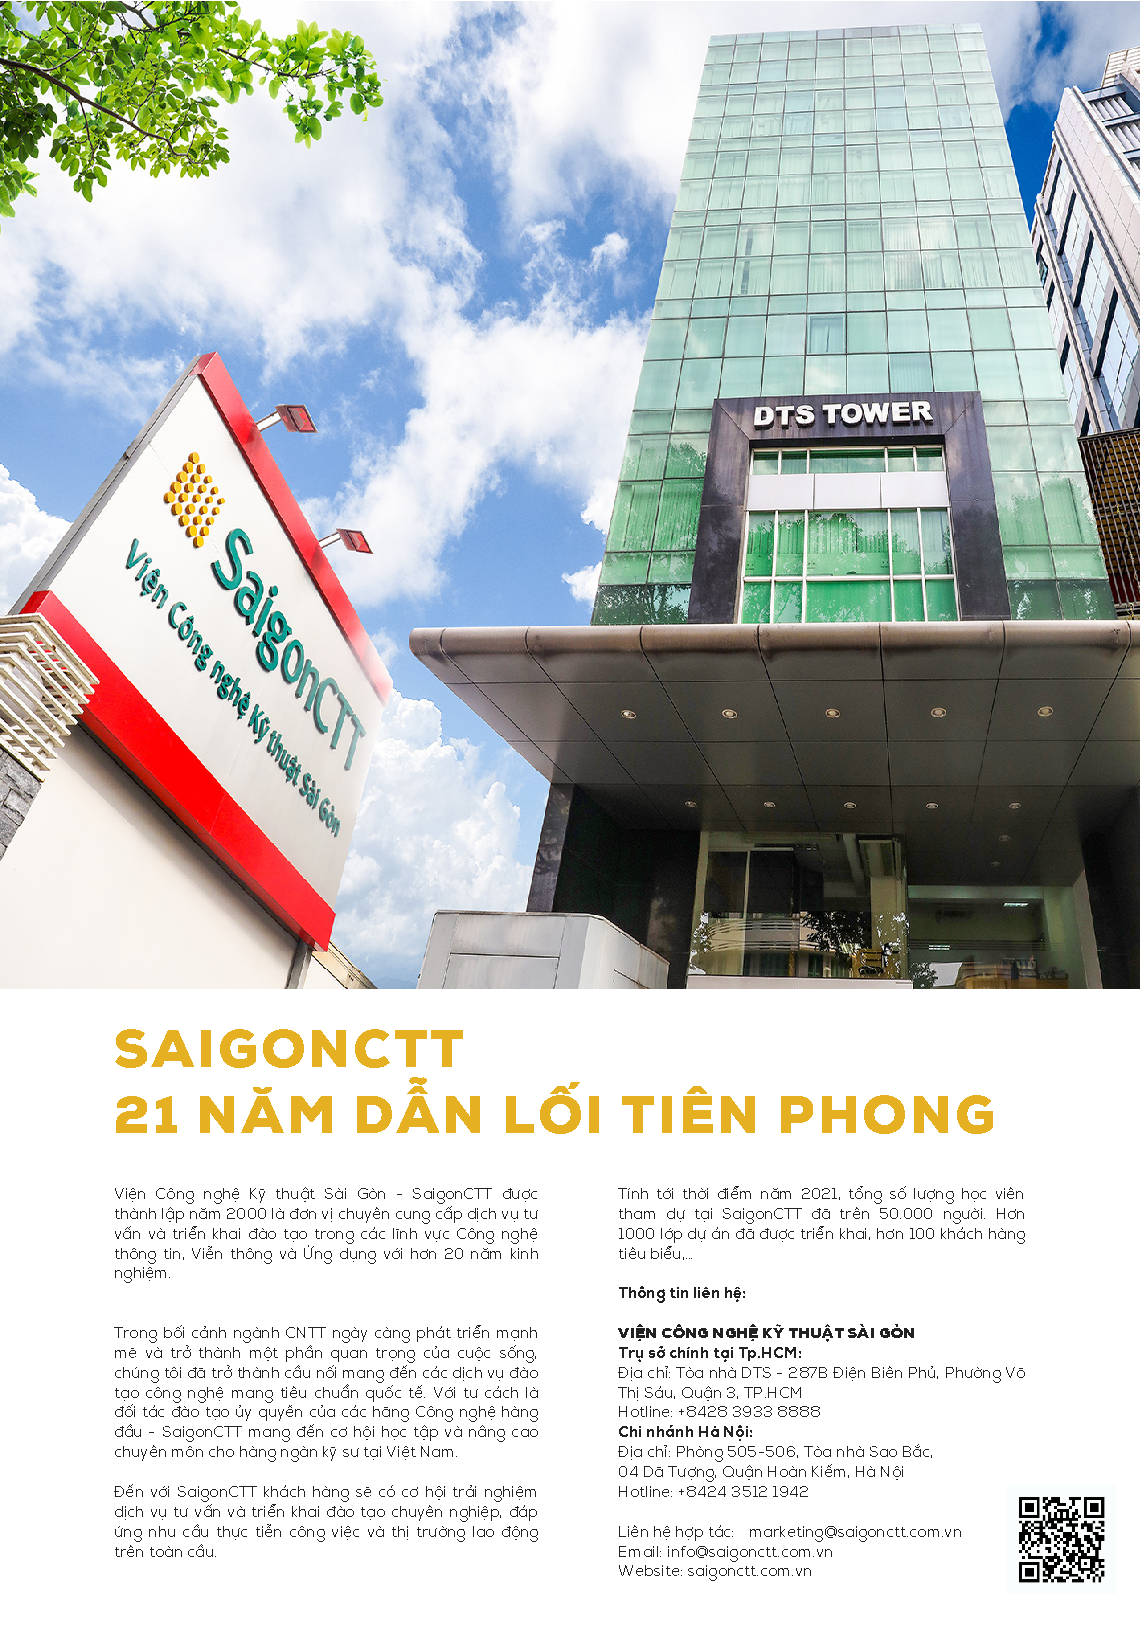
\includegraphics[scale=1]{DTS.pdf}}}
%	\centering
%	\vspace*{0cm}
%	\endgroup
%	\newpage	
%	\pagestyle{empty}
%	
	\setcounter{figure}{0}
	\thispagestyle{duongvaotoanhocnone}
\pagestyle{duongvaotoanhoc}
\everymath{\color{duongvaotoanhoc}}
\graphicspath{{../duongvaotoanhoc/pic2/}}
\blfootnote{$^1$\color{duongvaotoanhoc}Bài viết gốc: {Infinity Category Theory Offers a Bird's--Eye View of Mathematics}, đăng trên {Scientific American}, Volume $325$, Issue $4$, October $2021$.}
\blfootnote{$^2$\color{duongvaotoanhoc}Johns Hopkins University, chuyên gia về lý thuyết phạm trù bậc cao và lý thuyết đồng luân, các công trình của cô liên quan đến phạm trù mô hình và nền tảng của lý thuyết phạm trù vô cực}
\blfootnote{$^3$\color{duongvaotoanhoc}Universit\'e Paris--Saclay.}
\begingroup
\AddToShipoutPicture*{\put(0,616){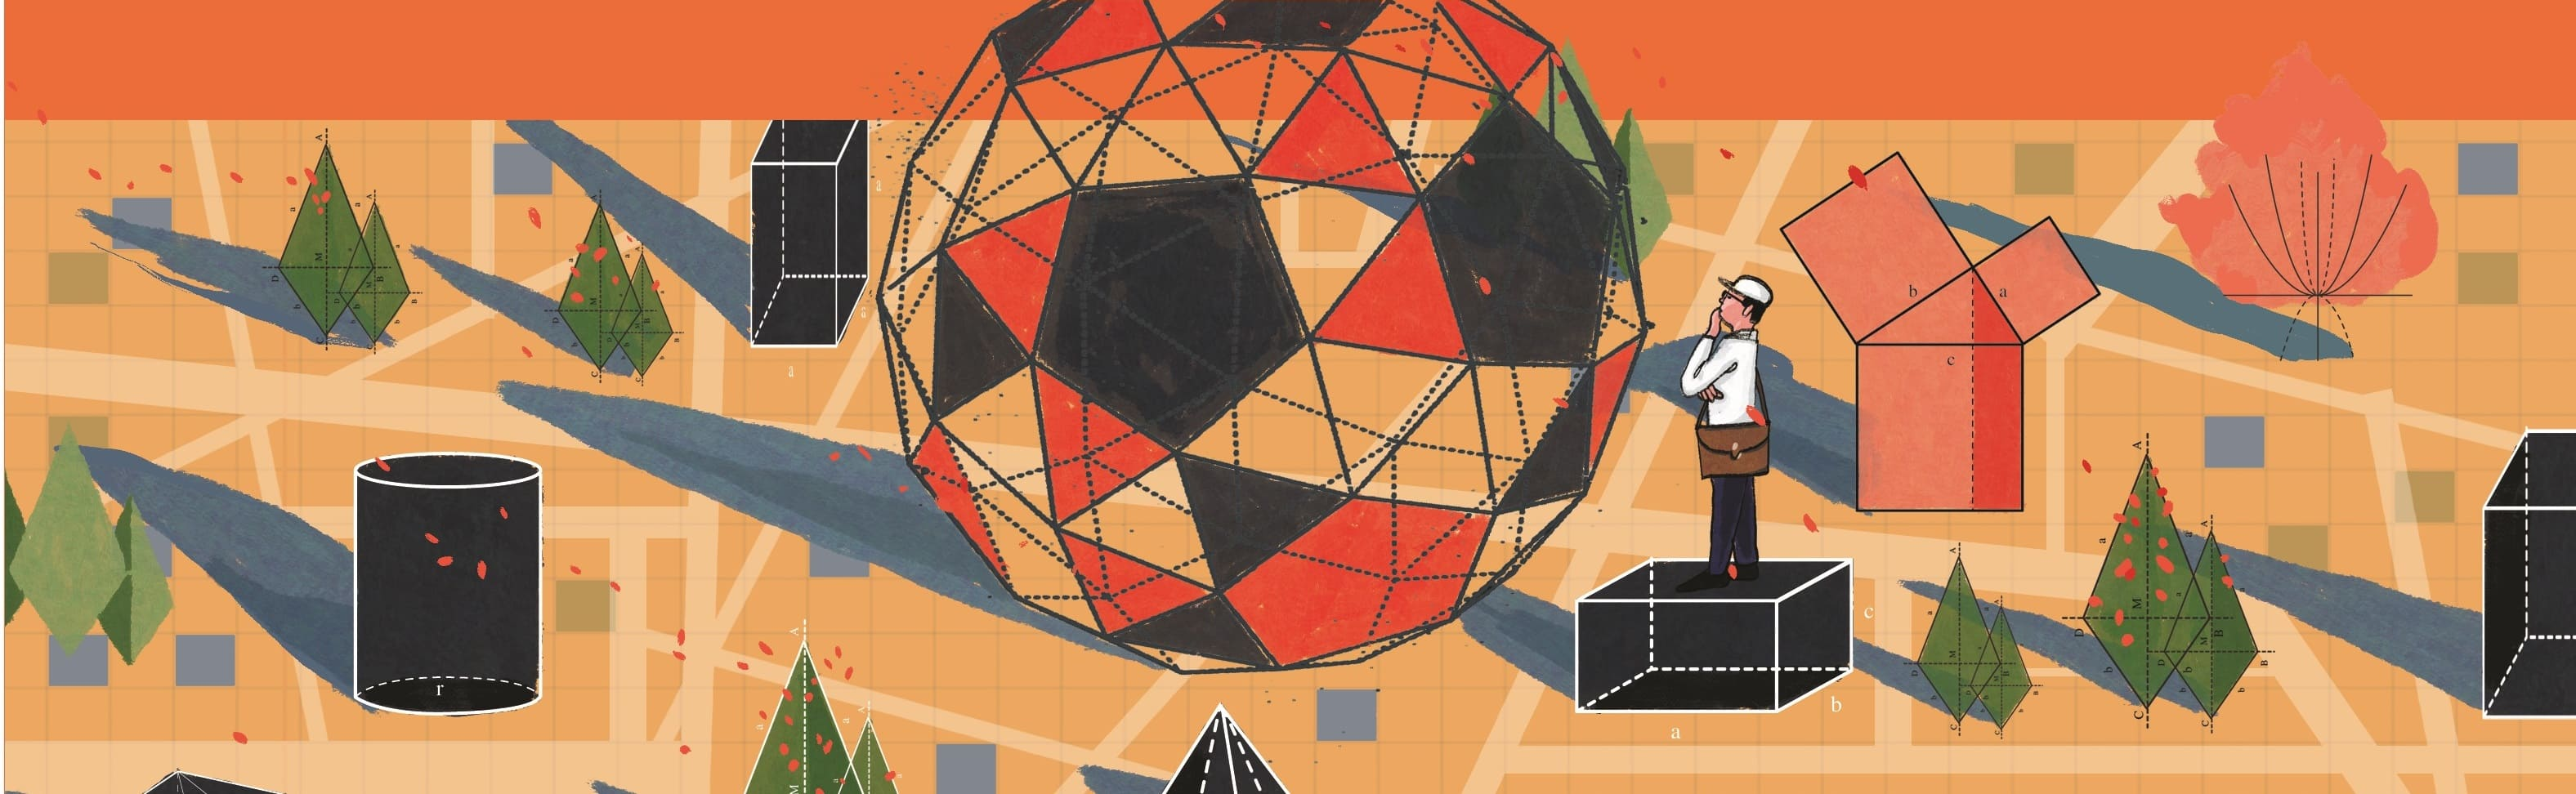
\includegraphics[width=19.3cm]{../bannerduongvao}}}
\AddToShipoutPicture*{\put(78,472){
\includegraphics[scale=1]{../tieude1.pdf}}}
\centering
\endgroup

\vspace*{235pt}

\begin{multicols}{2}	
	Một ngày thu ở New England, khi còn là sinh viên năm ba, tôi đi ngang qua một ga tàu điện ngầm và một bài toán đã lọt vào mắt tôi. Một người đàn ông cùng những ý tưởng được vẽ nguệch ngoạc trên tường, một trong số đó là bài toán dựng một hình lập phương với thể tích gấp đôi một hình lập phương khác cho trước, bằng thước thẳng và compa. 
	\vskip 0.1cm
	Điều này làm tôi phải dừng lại. Tôi đã thấy bài toán này trước đây, đó là một câu đố từ hơn hai thiên thiên kỷ trước, mà theo Plutarch thì tác giả là Plato. Một thanh thước thẳng (lý tưởng) cho phép kéo dài một đoạn thẳng theo cả hai hướng, và một chiếc compa cho phép vẽ một đường tròn với bán kính tùy ý và tâm cho trước. Cái khó của câu đố này là các điểm và độ dài được dựng ra sau cùng hoặc phải có từ đầu, hoặc phải được dựng từ những thông tin trước đó.
	\vskip 0.1cm
	Để gấp đôi thể tích của hình lập phương, ta bắt đầu với độ dài cạnh của nó. Ta hoàn toàn có thể xem độ dài này là $1$ vì đó là độ dài duy nhất được cho trước. Để dựng hình lập phương lớn, ta cần tìm cách dựng cạnh của nó với độ dài yêu cầu, ở đây là $\sqrt[3]{2}$, mà chỉ dùng thước thẳng và compa.
	\vskip 0.1cm
	Đây là một bài toán khó. Không ai giải được nó sau hơn $2000$ năm. Cuối cùng thì, vào năm $1837$, Pierre Laurent Wantzel đã giải thích tại sao chưa ai thành công, bằng cách chứng minh rằng bài toán không có lời giải. Chứng minh của ông sử dụng thứ toán học tối tân bấy giờ, được đặt nền móng bởi nhà toán học Pháp đương đại \'Evariste Galois, người đã chết ở tuổi $20$ trong một cuộc đấu súng mà có lẽ là vì một drama ngoại tình. Cũng ở tuổi $20$, bản thân tôi không đạt được những thành tựu toán học ấn tượng như vậy, nhưng ít nhất tôi cũng hiểu được chứng minh của Wantzel.
	\vskip 0.1cm
	Ý tưởng như sau: Cho trước một điểm làm gốc và một đoạn với độ dài $1$, ta dễ dàng dựng được tất cả các điểm trên trục số với tọa độ hữu tỷ (tất nhiên ta đã lờ đi, như các nhà toán học hay làm, sự thật rằng ta không thể vẽ vô hạn điểm trong thời gian hữu hạn).
	\vskip 0.1cm
	Wantzel đã chứng minh rằng, chỉ bằng những công cụ trên, mỗi điểm mới dựng phải là nghiệm của một phương trình đa thức bậc hai $ax^2 + bx + c = 0$ với các hệ số $a, b, c$ thu được từ các điểm đã dựng trước đó. Tuy nhiên, điểm $\sqrt[3]{2}$ lại là nghiệm của phương trình đa thức bậc ba $x^3 - 2 = 0$, và lý thuyết ``mở rộng trường" của Galois đã chứng minh một cách thuyết phục rằng bạn không thể thu được nghiệm của một đa thức bất khả quy bậc ba chỉ bằng cách giải các phương trình bậc hai, về cơ bản là vì $3$ không phải là lũy thừa của $2$.
	\begin{figure}[H]
		\centering
		\vspace*{-5pt}
		\captionsetup{labelformat= empty, justification=centering}
		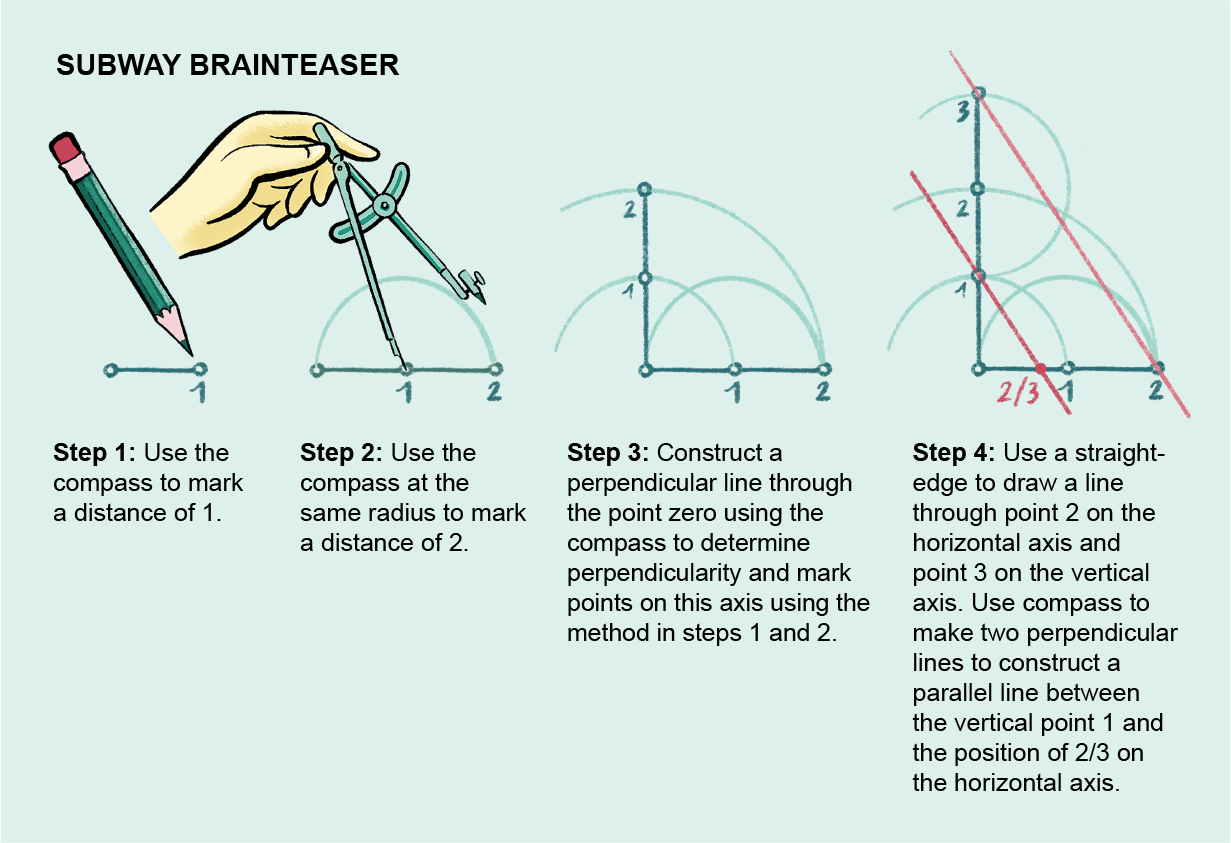
\includegraphics[width=1\linewidth]{1}
		\caption{\small\textit{\color{duongvaotoanhoc}Thước thẳng và compa cho phép dựng mọi số hữu tỷ.}}
		\vspace*{-10pt}
	\end{figure}
	Với ``vũ khí đầy mình'', tôi không kìm được mà lại gần người đàn ông trên đường. Đúng như dự đoán, nỗ lực giải thích, rằng vì sao tôi biết bài toán này không có lời giải, đã không đi tới đâu cả. Ngược lại, người đàn ông tuyên bố rằng những gì được dạy đã khiến tôi trở nên bảo thủ và không thể ``mở mang cái đầu ra''. Sau cùng, bạn gái đã kéo được tôi khỏi cuộc tranh cãi và chúng tôi tiếp tục đi.
	\vskip 0.1cm
	Nhưng vẫn còn đó một câu hỏi thú vị: Tại sao tôi, một đứa sinh viên năm ba vắt mũi chưa sạch, lại có thể học được cách dễ dàng thao túng các hệ thống số trừu tượng như các trường Galois chỉ trong vài tuần? Phần cuối của lớp học đó gồm nhóm đối xứng, vành đa thức và các cấu trúc liên quan, những thứ có lẽ sẽ làm đau đầu cả những người khổng lồ như Isaac Newton, Gottfried Leibniz, Leonhard Euler hay Carl Friedrich Gauss. Tại sao các nhà toán học lại có thể dạy cho các thế hệ sinh viên sau những khám phá làm kinh động cả những chuyên gia ở thế hệ trước?
	\begin{figure}[H]
		\centering
		\vspace*{-5pt}
		\captionsetup{labelformat= empty, justification=centering}
		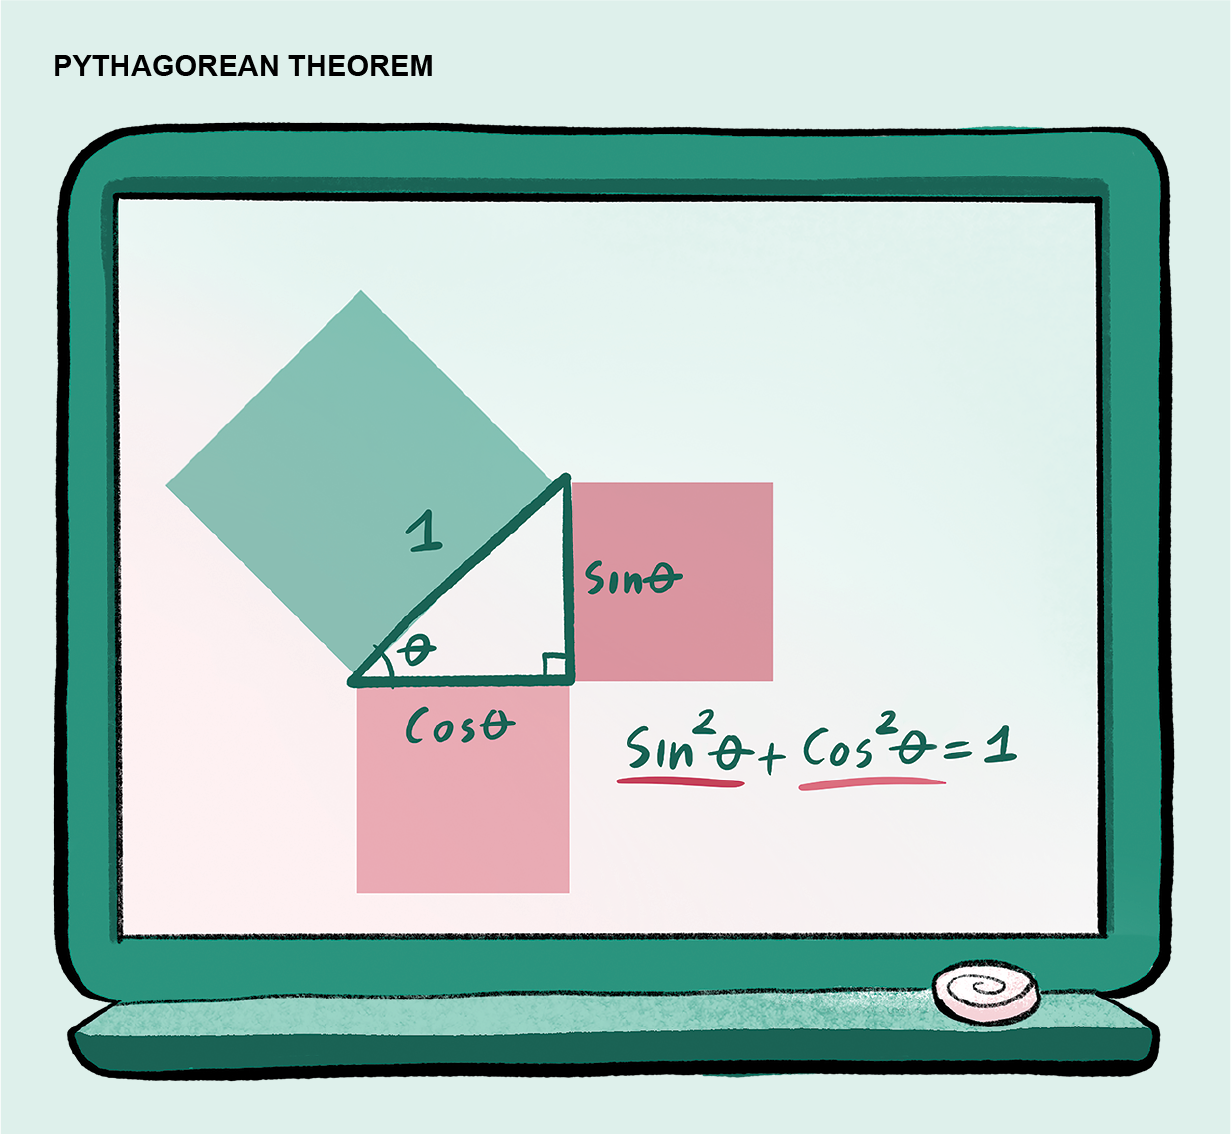
\includegraphics[width=1\linewidth]{2}
		\caption{\small\textit{\color{duongvaotoanhoc}Đẳng thức $\sin^2\theta + \cos^2\theta = 1$ từ định lý Pythagore.}}
		\vspace*{-10pt}
	\end{figure}
	Một phần câu trả lời đến từ những tiến bộ gần đây của toán học, thứ mang lại một cái nhìn ``từ trên xuống'', thông qua các cấp độ trừu tượng ngày càng tăng. Lý thuyết phạm trù là một nhánh toán học giải thích khi nào những đối tượng toán học khác nhau được coi là ``như nhau''. Định lý cơ bản của nó nói rằng bất kỳ đối tượng nào, bất kể phức tạp ra sao, đều hoàn toàn xác định khi biết quan hệ của nó với các đối tượng tương tự. Nhờ lý thuyết phạm trù, chúng ta dạy các nhà toán học trẻ những ý tưởng mới nhất bằng những quy tắc tổng quát có thể áp dụng cho những phạm trù khác nhau của toán học, thay vì đào sâu vào những quy luật đặc trưng chỉ áp dụng được trong một lĩnh vực đơn lẻ.
	\vskip 0.1cm
	Khi toán học liên tục tiến hóa, cảm nhận của các nhà toán học về sự ``như nhau'' của hai vật cũng mở rộng theo. Trong vài thập kỷ vừa qua, tôi cùng nhiều nhà nghiên cứu đang phát triển lý thuyết phạm trù để hợp lý hóa khái niệm ``duy nhất'' mới này. Những phạm trù mới, gọi là phạm trù vô cực ($\infty$--phạm trù), đã mở rộng lý thuyết phạm trù lên vô hạn chiều. Ngôn ngữ $\infty$--phạm trù mang lại cho các nhà toán học những công cụ mạnh mẽ để nghiên cứu những bài toán mà quan hệ giữa các vật quá rắc rối để có thể định nghĩa bằng phạm trù cổ điển. Góc nhìn ``thu nhỏ đến vô hạn'' này mang lại một cách nghĩ mới mẻ cho những khái niệm cũ cũng như một con đường để khám phá những khái niệm mới.
	\vskip 0.1cm
	\textbf{\color{duongvaotoanhoc}Phạm trù}
	\vskip 0.1cm
	Giống như nhiều đồng nghiệp của mình, tôi bị toán học lôi cuốn phần vì trí nhớ tệ của mình. Điều này có thể làm nhiều người bối rối khi họ nhớ rằng môn toán ở phổ thông là một mớ công thức phải thuộc -- các đẳng thức lượng giác chẳng hạn. Nhưng tôi lại thấy chúng rất dễ chịu vì hầu hết những công thức thường dùy đều có thể rút ra từ $\sin^2 \theta + \cos^2 \theta = 1$, đẳng thức mà tự thân nó có một kiến giải hình học tao nhã: đó chỉ là hệ quả trực tiếp của định lý Pythagore cho tam giác vuông với cạnh huyền bằng $1$ và một góc nhọn bằng $\theta$.
	\vskip 0.1cm
	Viễn cảnh toán học lý tưởng này, nơi mà mọi thứ đều ``hợp lý'' và chẳng cần ghi nhớ gì hết, đã phần nào đó sụp đổ ở cấp đại học. Lúc này, sinh viên được biến đến một rổ đối tượng toán học được triệu hồi từ vài thế kỷ trước. ``Nhóm'', ``vành'' và ``trường'' thuộc về lĩnh vực toán học được gọi là Đại số, một từ có nguồn gốc từ cuốn sách viết ở thế kỷ IX bởi nhà toán học, thiên văn học Ba Tư Muhammad ibn Musa al--Khwarizmi, mà tựa sách dịch ra đại khái là "Khoa học của phục hồi và cân bằng". Suốt thiên niên kỷ sau đó, đại số đã tiến hóa từ việc nghiên cứu bản chất nghiệm của các hệ phương trình đa thức thành nghiên cứu các hệ thống số trừu tượng. Vì không có số thực $x$ nào thỏa mãn phương trình $x^2+1 = 0$, các nhà toán học đã tạo ra một hệ thống số mới -- mà ngày nay gọi là số phức -- bằng cách thêm một số ảo $i$ và quy định rằng $i^2+1 = 0$.
	\vskip 0.1cm
	Đại số chỉ là một trong nhiều môn học ở chương trình toán đại học. Những môn cơ bản khác gồm Tôpô học -- nghiên cứu trừu tượng về các không gian -- và Giải tích, môn học bắt đầu với việc chặt chẽ hóa các tính toán trên hàm thực, trước khi rẽ sang những miền đất xa lạ hơn như không gian xác suất, biến ngẫu nhiên, đa tạp phức hay hàm chỉnh hình. Làm sao để sinh viên có thể thấy tất cả chúng đều hợp lý?
	\begin{figure}[H]
		\centering
		\vspace*{-5pt}
		\captionsetup{labelformat= empty, justification=centering}
		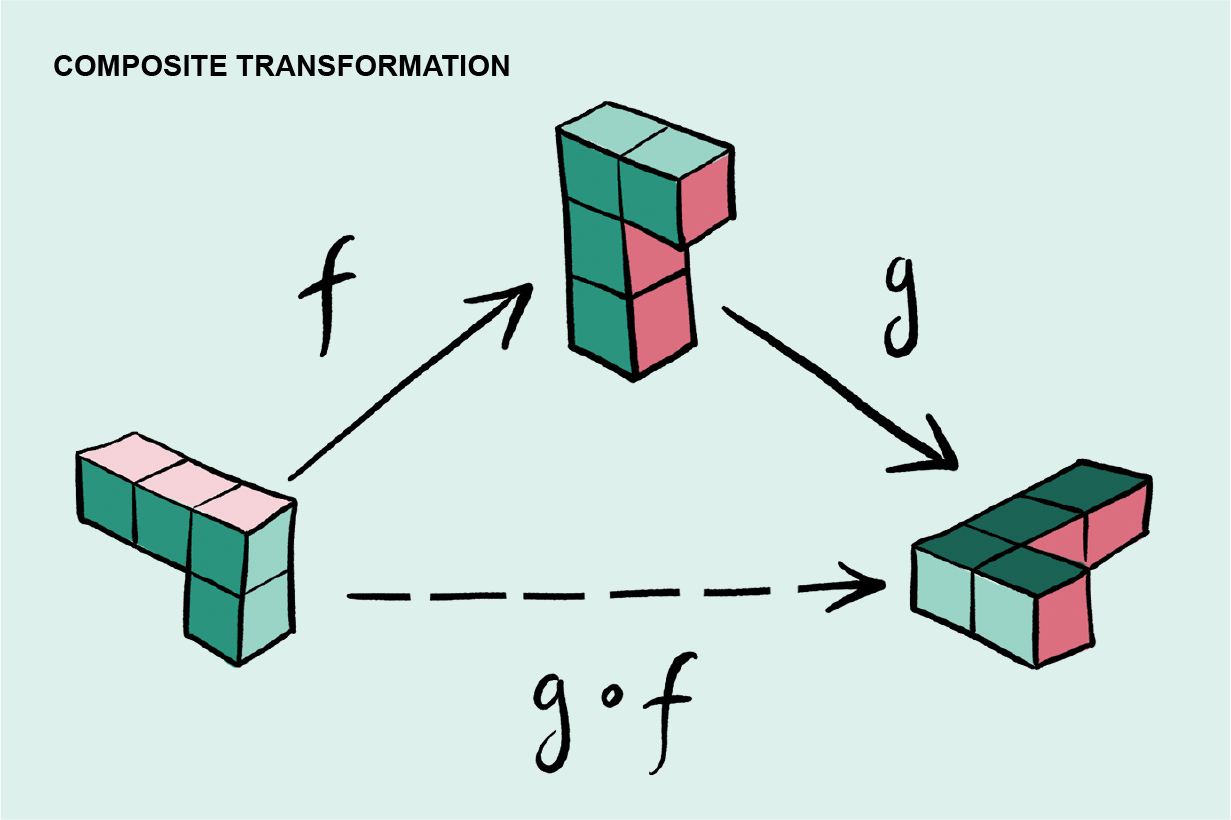
\includegraphics[width=1\linewidth]{3}
		\caption{\small\textit{\color{duongvaotoanhoc}Hợp thành của hai phép biến đổi là một phép biến đổi mới.}}
		\vspace*{-10pt}
	\end{figure}
	Một ý tưởng toán học nghe có vẻ mâu thuẫn là đơn giản hóa bằng cách trừu tượng hóa. Như Eugenia Cheng đã viết trong ``The Art of Logic in an Illogical World'' (Nghệ thuật của logic trong một thế giới phi logic), ``một trong những sức mạnh của trừu tượng hóa là nhiều bối cảnh khác nhau trở nên giống nhau khi bạn quên đi một số chi tiết.'' Đại số hiện đại được tạo ra đầu thế kỷ XX khi các nhà toán học quyết định thống nhất nghiên cứu của họ trên nhiều ví dụ khác nhau về các cấu trúc đại số xuất hiện khi xem xét nghiệm của các hệ phương trình đa thức hay các cấu hình trong mặt phẳng. Để liên kết việc tìm hiểu các cấu trúc này, họ xác định các ``tiên đề'' mô tả những tính chất chung của chúng. Nhóm, vành và trường đã được đưa vào thế giới toán học, cùng ý tưởng rằng một đối tượng toán học có thể được mô tả bằng những tính chất nó có và được khám phá một cách ``trừu tượng'', không phụ thuộc vào bối cảnh của những ví dụ hay xây dựng cụ thể.
	\vskip 0.1cm
	John Horton Conway đã có một suy nghĩ nổi tiếng về bản thể luận kỳ lạ của các sự vật toán học: ``Chúng chắc chắn có tồn tại, nhưng bạn không thể động chạm gì mà chỉ có thể nghĩ về chúng. Điều này thật đáng kinh ngạc, và tôi vẫn chưa hiểu, dù đã là nhà toán học suốt cuộc đời mình. Rằng làm thế nào một sự vật có thể ở đó mà lại không thực sự ở đó?''
	\begin{figure}[H]
		\centering
		\vspace*{-5pt}
		\captionsetup{labelformat= empty, justification=centering}
		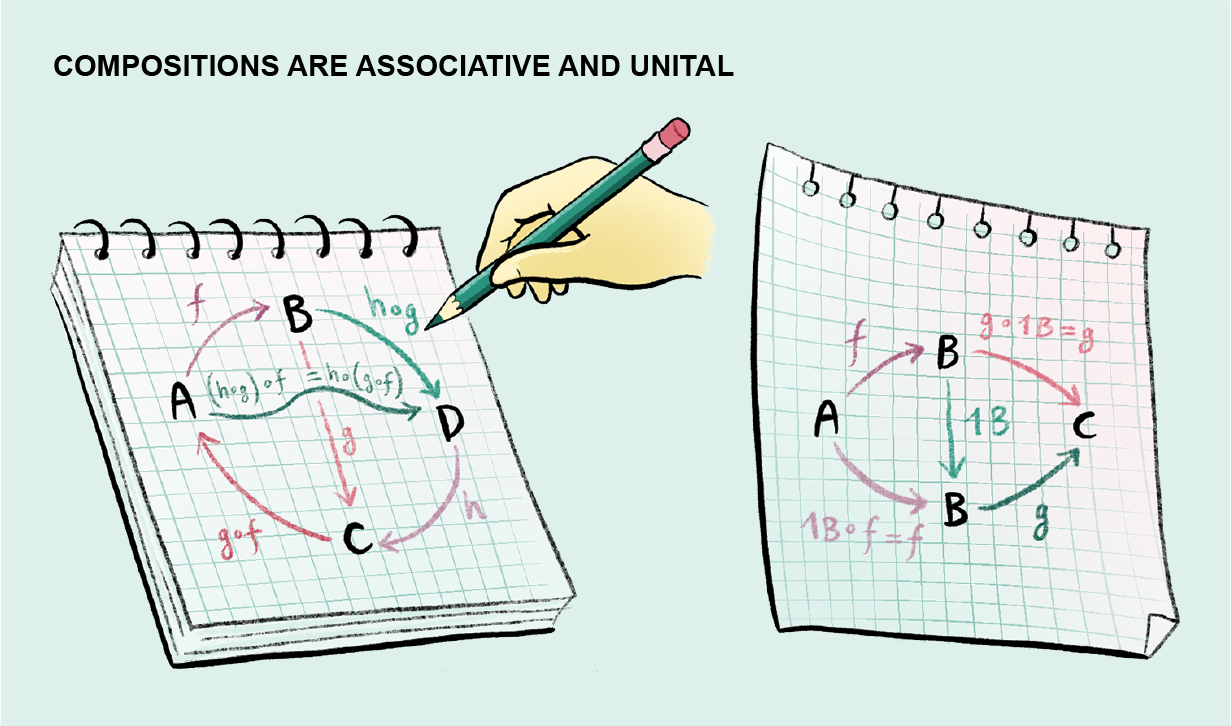
\includegraphics[width=1\linewidth]{4}
		\caption{\small\textit{\color{duongvaotoanhoc}Phép hợp thành có tính kết hợp và có đơn vị.}}
		\vspace*{-10pt}
	\end{figure}
	Nhưng thế giới của các đối tượng toán học tồn--tại--mà--không--thực--sự--ở--đó này có một vấn đề: Nó quá lớn cho bất kỳ ai để có thể hiểu được. Ngay trong đại số thôi đã có quá nhiều sự vật toán học để nghiên cứu, nhưng lại có quá ít thời gian để thể có thể thấy thấy cả đều hợp lý. Vào khoảng thế kỷ XX, các nhà toán học bắt đầu nghiên cứu đại số phổ dụng,  gồm một ``tập hợp'', có thể là một họ những phép đối xứng, những con số trong một hệ thống hoặc thứ gì đó hoàn toàn khác, cùng một số phép toán -- chẳng hạn như phép cộng và phép nhân -- thỏa mãn một loạt các tiên đề liên quan như tính kết hợp, tính giao hoán hay tính phân phối. Với những điều chỉnh khác nhau như: ``Phép toán được định nghĩa cục bộ hay toàn cục?'', ``Nó có khả nghịch không?'', người ta thu được những cấu trúc đại số cơ bản: nhóm, vành và trường. Nhưng toán học thì không bị hạn chế bởi những điều chỉnh này, điều này cho thấy một phần rất nhỏ so với số lượng vô hạn các khả năng có thể xảy ra.
	\vskip 0.1cm
	Sự sinh sôi của các đối tượng toán học trừu tượng mới mang lại sự phức tạp cho chính chúng. Một cách để đơn giản hóa là trừu tượng hóa hơn nữa, đến mức ta có thể chứng minh các định lý cho hàng loạt đối tượng cùng lúc mà không cần biết rằng cụ thể chúng ta nói về loại đối tượng nào.
	\vskip 0.1cm
	Lý thuyết phạm trù, ra đời vào những năm $40$ bởi Samuel Eilenberg và Saunders Mac Lane, đã làm chính việc này. Dù ban đầu nó được đưa ra để định nghĩa chặt chẽ thuật ngữ lỏng lẻo hay dùng là ``tương đương tự nhiên'', nó còn mang lại một cách nghĩ phổ quát về đại số phổ dụng cũng như các ngành toán học khác. Với ngôn ngữ cua Eilenberg và Mac Lane, ngày nay ta hiểu rằng mỗi loại đối tượng toán học đều thuộc về một phạm trù riêng, được định nghĩa là một họ các ``vật'' cùng các phép biến đổi được vẽ dưới dạng ``mũi tên'' giữa các vật. Chẳng hạn, trong đại số tuyến tính, người ta nghiên cứu các không gian véc tơ trừu tượng như không gian Euclid $3$--chiều. Các phép biến đổi tương ứng được gọi là các biến đổi tuyến tính, và mỗi phép biến đổi phải có một không gian nguồn và một không gian đích (đầu vào và đầu ra của phép biến đổi). Cũng như các hàm số, các phép biến đổi trong một phạm trù có thể ``hợp thành'' với nhau, nghĩa là ta áp dụng một phép biến đổi lên kết quả một phép biến đổi khác. Cho một cặp phép biến đổi $f: A \to B$ (đọc là ``$f$ là một phép biến đổi từ $A$ vào $B$'') và $g: B \to C$, quy tắc của phạm trù trả về một phép biến đổi hợp thành duy nhất, ký hiệu bởi $g \circ f: A \to C$ (đọc là ``$g$ hợp $f$ là một phép biến đổi từ $A$ vào $C$''). Cuối cùng, quy tắc hợp thành này có tính kết hợp, nghĩa là $h \circ (g \circ f) = (h \circ g) \circ f$. Nó cũng có đơn vị: mỗi vật $B$ đều có một ``biến đổi đồng nhất", thường ký hiệu bởi $\pmb{1}_B$, thỏa mãn tính chất $g \!\circ\! \pmb{1}_B \!=\! g$ và $\pmb{1}_B \!\circ\! f \!=\! f$ với mọi phép biến đổi $g$ và $f$ lần lượt có nguồn và đích là $B$. 
	\vskip 0.1cm
	Làm thế nào mà các phạm trù có thể giúp cô hay cậu sinh viên bất hạnh, người đã phải gặp quá nhiều đối tượng toán học và chẳng có đủ thời gian học hết? Bất kỳ lớp cấu trúc nào trong đại số phổ dụng có thể khác các lớp khác, nhưng các phạm trù chứa chúng thì rất giống nhau, theo một cách có thể diễn tả chính xác bằng ngôn ngữ phạm trù.
	\vskip 0.1cm
	Với đủ kinh nghiệm, một nhà toán học sẽ biết rằng họ sẽ thấy gì khi gặp một kiểu đổi tượng đại số mới. Ý tưởng này được thể hiện trong các sách toán hiện đại mà lý thuyết nhóm, vành và không gian véctơ được trình bày theo một chuỗi, về cơ bản là các lý thuyết đó song song với nhau. Có những sự tương tự khác, lỏng lẻo hơn, giữa những những phạm trù này và một số phạm trù mà sinh viên gặp trong các môn tôpô hay giải tích, và những sự tương đồng đó đó giúp họ tiếp thu tài liệu mới nhanh hơn. Những khuôn mẫu như vậy cho phép sinh viên có thêm thời gian khám phá các chủ đề cụ thể có vai trò phân biệt các lĩnh vực của toán học -- mặc dù những tiến bộ trong nghiên cứu toán học thường đến từ những sự tương tự mới và đáng ngạc nhiên giữa hai lĩnh vực không liên quan trước đó.
	\vskip 0.1cm
	\textbf{\color{duongvaotoanhoc}Đối xứng}
	\vskip 0.1cm
	Các tầng trừu tượng, từ những cấu trúc toán học cụ thể đến những hệ tiên đề và sau đó là các vật trong phạm trù, mở ra một thách thức mới: sự ``như nhau'' giữa một vật và một vật khác không còn rõ ràng nữa. Chẳng hạn, một nhóm, đối tượng toán học được cho bởi một họ trừu tượng các phép đối xứng mà các phần tử của nó được Amie Wilkinson (Đại học Chicago) mô tả như những ``chuyển động'' lật hoặc xoay một đối tượng để đưa nó về trạng thái gần giống như ban đầu.
	\vskip 0.1cm
	Chẳng hạn, ta có thể khám phá các phép đối xứng của một chiếc áo thun. Có một phép đối xứng được coi là ``chuyển động đồng nhất'', khi mà người mặc chỉ đơn thuần là giữ chiếc áo thun như bình thường. Một phép đối xứng khác ứng với chuyển động mà người mặc bỏ tay ra khỏi tay áo, giữ áo ở cổ, xoay áo $180$ độ và cho tay vào tay áo đối diện: mặt phải của áo vẫn ở ngoài nhưng áo được mặc ngược ra sau. Một phép đối xứng khác nữa ứng với chuyển động mà người mặc cởi áo ra, lộn mặt trong ra ngoài và mặc lại sao cho mỗi tay ở đúng tay áo ban đầu.  Lúc này chiếc áo thun bị lộn ngược trong ra ngoài và sau ra trước. Một phép đối xứng cuối cùng là kết hợp hai chuyển động trên: không giống như với phần lớn các nhóm, hai chuyển động này có thể thực hiện theo thứ tự tùy ý mà không làm thay đổi kết quả. Mỗi một trong bốn chuyển động trên được coi là một phép đối xứng vì sau cùng chiếc áo thun được mặc nói chung là giống như lúc đầu.
	\begin{figure}[H]
		\centering
		\vspace*{-5pt}
		\captionsetup{labelformat= empty, justification=centering}
		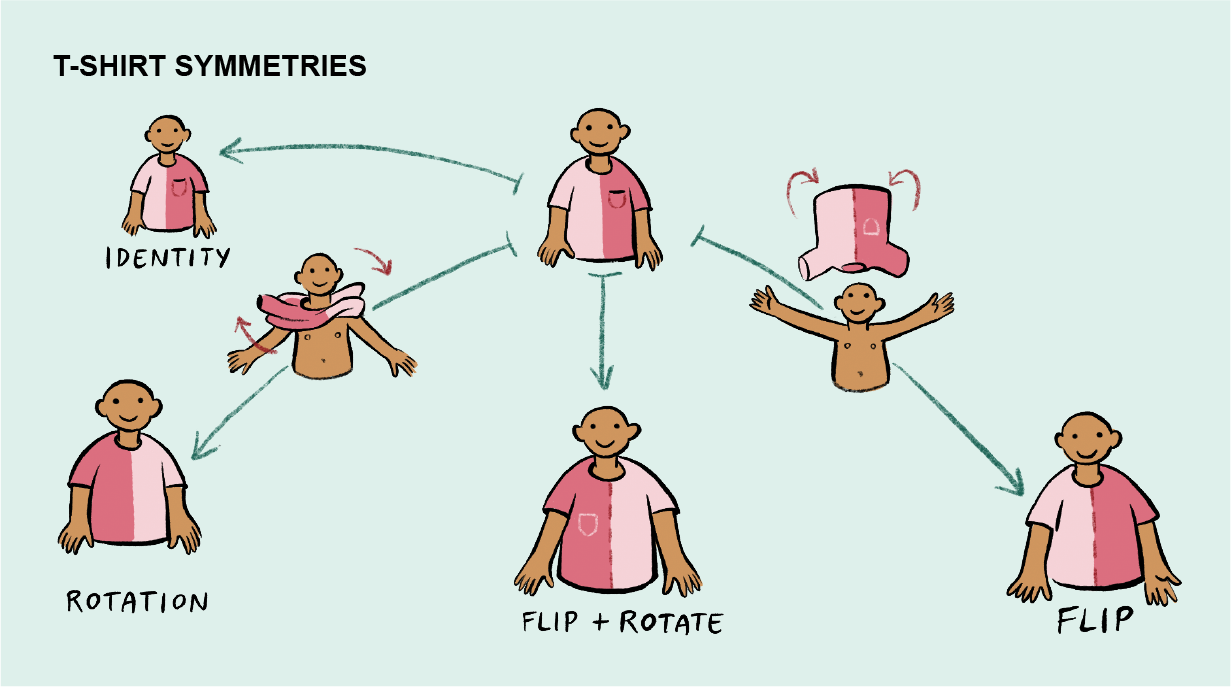
\includegraphics[width=1\linewidth]{5}
		\caption{\small\textit{\color{duongvaotoanhoc}Các phép đối xứng trên áo thun.}}
		\vspace*{-10pt}
	\end{figure}
	Một nhóm khác là ``nhóm lật thảm'', nó mô tả các đối xứng của một tấm thảm. Bên cạnh chuyển động đồng nhất (tức là giữ nguyên tấm thảm), ta có thể xoay nó $180$ độ, hoặc lật mặt dưới lên trên, hoặc kết hợp cả hai (tấm thảm nói chung không phải là hình vuông, nhưng nếu nó là hình vuông thì ta sẽ có nhiều phép đối xứng hơn nữa). Dù chiếc áo thun chẳng liên quan gì đến tấm thảm, có một trực giác rằng hai nhóm đối xứng trên có cùng ``dạng'' với nhau. Thứ nhất, cả hai nhóm đều có cùng số chuyển động (ở đây là bốn) và quan trọng hơn là ta có thể ghép mỗi chuyển động ở nhóm áo thun với nhóm lật thảm sao cho phép hợp thành chuyển động ở hai nhóm tương thích với nhau. Nói cách khác, ta có thể ghép cặp các chuyển động ở hai nhóm (phép đồng nhất ghép với phép đồng nhất, phép lật ghép với phép lật, phép xoay ghép với phép xoay, và cứ như vậy). Thứ hai, nếu ta lấy hai chuyển động từ một nhóm và thực hiện chúng theo trình tự, kết quả thu được sẽ giống với kết quả khi ta thực hiện hai chuyển động tương ứng từ nhóm còn lại theo trình tự. Về mặt kỹ thuật, các nhóm này được liên kết với nhau bởi một ``đẳng cấu'' (isomorphism), thuật ngữ được tạo ra bằng cách ghép từ gốc Hy Lạp \emph{isos}, nghĩa là ``bằng'', với \emph{morphe}, nghĩa là ``dạng''.
	\vskip 0.1cm
	Ta có thể định nghĩa đẳng cấu trong bất kỳ phạm trù nào, cho phép ta chuyển khái niệm này giữa các ngữ cảnh toán học khác nhau. Một đẳng cấu giữa hai vật $A$ và $B$ trong một phạm trù được cho bởi một cặp biến đổi $f: A \to B$ và $g: B \to A$ với sao cho các phép biến đổi hợp thành $g \circ f$ và $f \circ g$ lần lượt là các biến đổi đồng nhất $\pmb{1}_A$ và $\pmb{1}_B$. Trong phạm trù các không gian tôpô, khái niệm đẳng cấu được mô tả bởi một cặp hàm liên tục nghịch đảo lẫn nhau. Chẳng hạn, có một phép biến dạng liên tục cho phép bạn biến đổi một chiếc bánh vòng (chưa nướng) thành hình dạng như tách cà phê: lỗ ở giữa chiếc bánh vòng trở thành quai cầm, và phần cốc được tạo thành bằng cách dùng ngón tay ép. (Để phép biến dạng là liên tục, bạn không được xé rách chiếc bánh, đó là lý do vì sao không nên nướng bánh trước khi làm trò này.)
	\vskip 0.1cm
	Ví dụ này dẫn đến câu đùa rằng nhà tôpô học không thể phân biệt giữa tách cà phê và chiếc bánh vòng: với tư cách là các không gian trừu tượng, hai đối tượng này giống nhau. Trên thực tế, nhiều nhà tôpô học có khả năng phân biệt còn tệ hơn thế nữa kia; đó là vì họ đã sử dụng một quy ước linh hoạt hơn nhiều để mô tả tình huống khi hai không gian là ``như nhau'', họ đồng nhất hai không gian bất kỳ mà chỉ ``tương đương đồng luân'' với nhau thôi. Thuật ngữ trên là khái niệm đẳng cấu trong một phạm trù kỳ lạ hơn, phạm trù đồng luân của các không gian. Một tương đương đồng luân là một kiểu biến dạng liên tục khác, nhưng lúc này bạn được phép dính hai điểm phân biệt với nhau. Chẳng hạn, tưởng tượng rằng bạn bắt đầu với chiếc quần jean và thu gọn chiều dài của hai ống quần đến khi bạn thu được chiếc quần lọt khe, một ``không gian'' khác mà cấu trúc tôpô về cơ bản là không đổi -- nó vẫn có hai lỗ để cho chân vào, dù hai ống quần ($2$--chiều) ban đầu đã bị rút thành hai vòng dây ($1$--chiều).
	\begin{figure}[H]
		\centering
		\vspace*{-5pt}
		\captionsetup{labelformat= empty, justification=centering}
		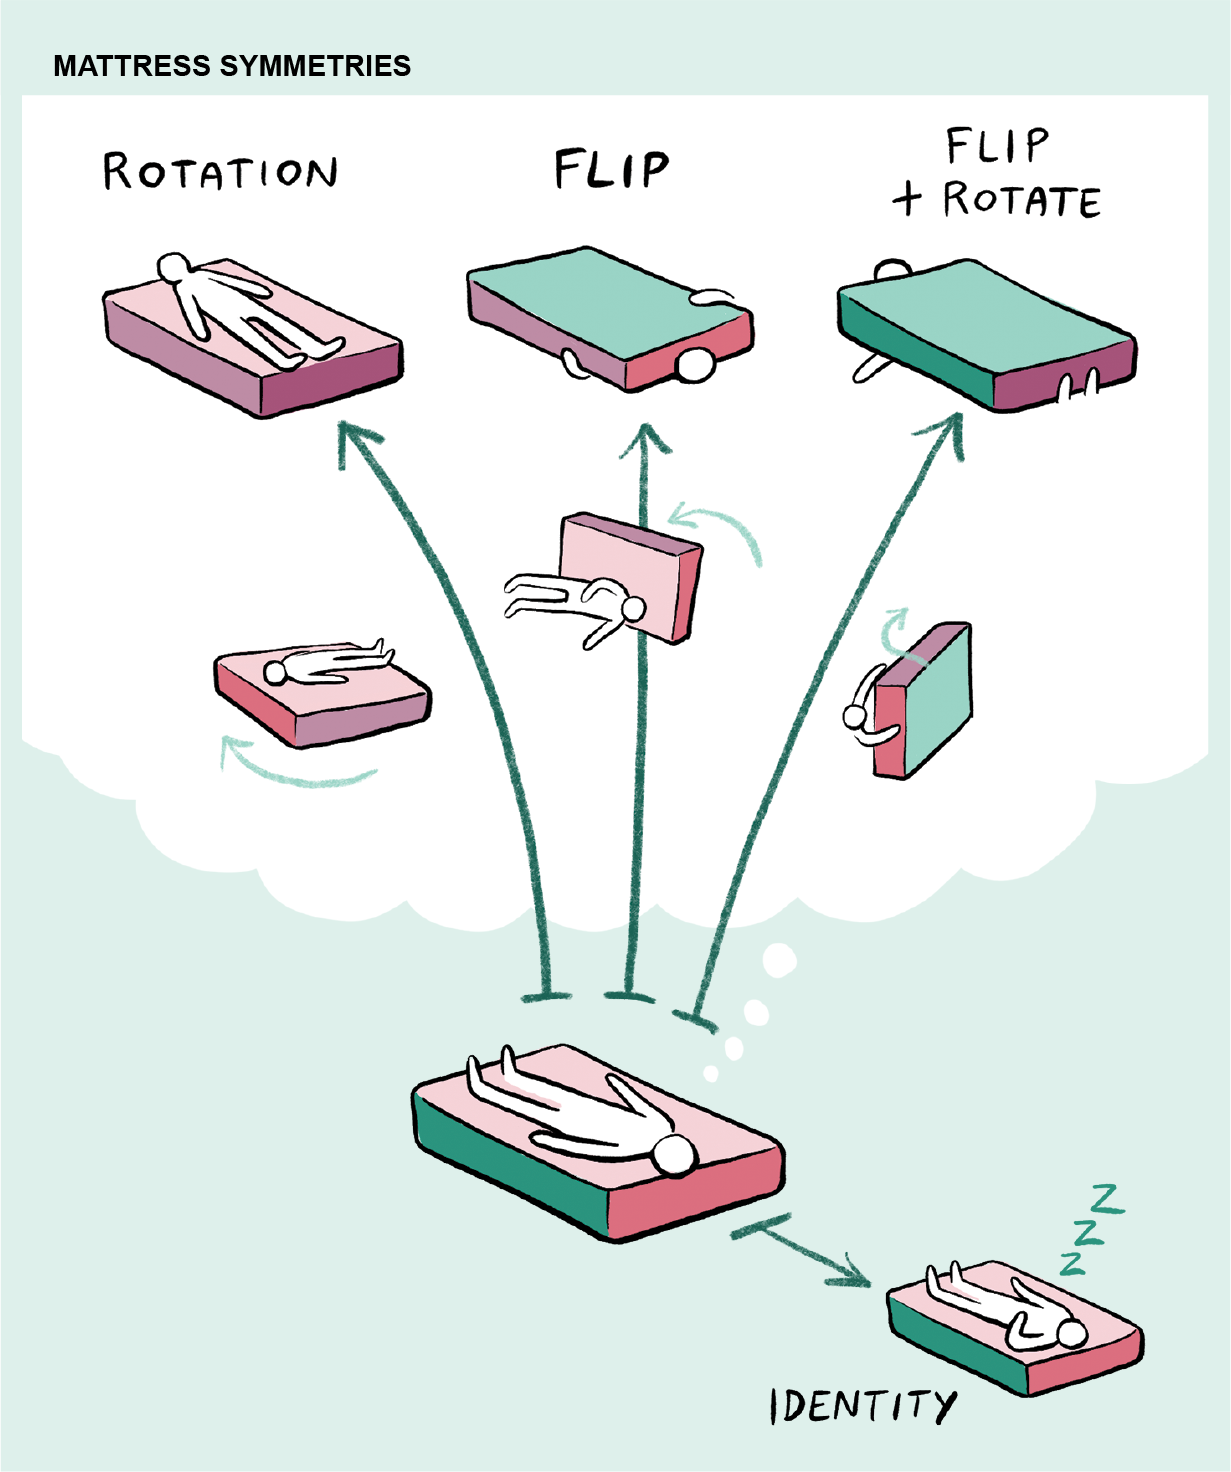
\includegraphics[width=1\linewidth]{6}
		\caption{\small\textit{\color{duongvaotoanhoc}Các phép đối xứng trên tấm thảm.}}
		\vspace*{-10pt}
	\end{figure}
	Một phép tương đương đồng luân khác thu hết toàn bộ không gian Euclid vô hạn $3$--chiều về một điểm bằng một vụ nổ ``Big Bang ngược'', khi mọi điểm đều thu về gốc, với tốc độ tăng dần theo khoảng cách giữa điểm đó với vị trí ban đầu của vụ nổ. 
	\vskip 0.1cm
	Trực giác rằng ta có thể dùng các vật đẳng cấu để thay thế nhau mà về cơ bản không làm thay đổi bản chất của phép xây dựng hay suy luận, là một trực giác rất mạnh mà các nhà lý thuyết phạm trù đã phải định nghĩa lại từ ``the'' trong tiếng Anh bởi thứ mà gần giống như từ ``$a$''. Chẳng hạn, có một khái niệm gọi là hợp rời của hai tập hợp $A$ và $B$. Giống như hợp thông thường, hợp rời $A \sqcup B$ chứa một bản sao của mỗi phần tử của $A$ cũng như của $B$. Nó khác hợp thông thường ở chỗ, nếu $A$ và $B$ có phần tử chung thì hợp rời $A \sqcup B$ chứa tới hai bản sao của phần tử đó, một bản sao ``nhớ'' rằng nó đến từ $A$ và bản sao còn lại nhớ rằng nó đến từ $B$.
	\vskip 0.1cm
	Có nhiều cách khác nhau để xây dựng hợp rời từ các tiên đề của lý thuyết tập hợp, chúng không cho chính xác cùng một tập hợp, nhưng sẽ cho các tập hợp đẳng cấu với nhau. Thay vì tốn thời gian tranh luận rằng cách xây dựng nào là chính tắc nhất, sẽ tiện hơn khi cứ giấu nhẹm sự mơ hồ này và dùng từ (the) hợp rời để chỉ bất kỳ tập hợp nào thỏa mãn bài toán phổ dụng tương ứng. Một ví dụ khác, các nhóm đối xứng áo thun và nhóm lật thảm ở trên đều được gọi là (the) nhóm bốn Klein.
	\vskip 0.1cm
	\textbf{\color{duongvaotoanhoc}Phạm trù vô cực}
	\vskip 0.1cm
	Có câu chuyện truyền miệng sau về nguồn gốc của định lý cơ bản của lý thuyết phạm trù: một nhà toán học trẻ tên Nobuo Yoneda đã mô tả một ``bổ đề'', tức là một định lý bổ trợ, cho Mac Lane ở điểm tàu Gare du Nord ở Paris năm $1954$. Yoneda bắt đầu giải thích bổ đề trên sân ga và tiếp tục ở trên tàu trước khi nó rời ga. Hệ quả của bổ đề này là mọi vật trong bất kỳ phạm trù nào đều hoàn toàn xác khi biết quan hệ của nó với các vật khác trong phạm trù đó, tức là các phép biến đổi từ vật đó vào vật khác hoặc ngược lại. Như vậy ta có thể đặc trưng một không gian tôpô $X$ bằng các nghiên cứu các hàm liên tục $f: T \to X$ đến từ các không gian $T$ khác. Chẳng hạn, một điểm trong $X$ ứng với một hàm liên tục $x: \ast \to X$ mà không gian nguồn $\ast$ là không gian với duy nhất một điểm. Ta có thể biết $X$ liên thông hay không bằng cách xét các ánh xạ $p: I \to X$ với nguồn là đoạn $I = [0,1]$. Một ánh xạ như thế là một ``đường'' có tham số trong không gian $X$ từ điểm $p(0)$ đến điểm $p(1)$, có thể xem như một quỹ đạo khả dĩ mà một con kiến có thể di chuyển trong $X$.
	\vskip 0.1cm
	Ta có thể dùng các điểm và đường trong một không gian để dịch các bài toán tôpô sang đại số: Mỗi không gian tôpô $X$ có một phạm trù tương ứng $\pi_1 X$, gọi là ``phỏng nhóm cơ bản'' của $X$. Vật trong phạm trù này là các điểm của không gian, và các phép biến đổi là các đường. Nếu một đường có thể biến dạng thành một đường khác mà vẫn cố định hai đầu mút, ta quy ước rằng hai đường này định nghĩa cùng một phép biến đổi. Các biến dạng này được gọi là các phép đồng luân, ta cần chúng để mô tả phép hợp thành của đường sao cho tính kết hợp được thỏa mãn, điều kiện cần của mọi phạm trù.
	\begin{figure}[H]
		\centering
		\vspace*{-5pt}
		\captionsetup{labelformat= empty, justification=centering}
		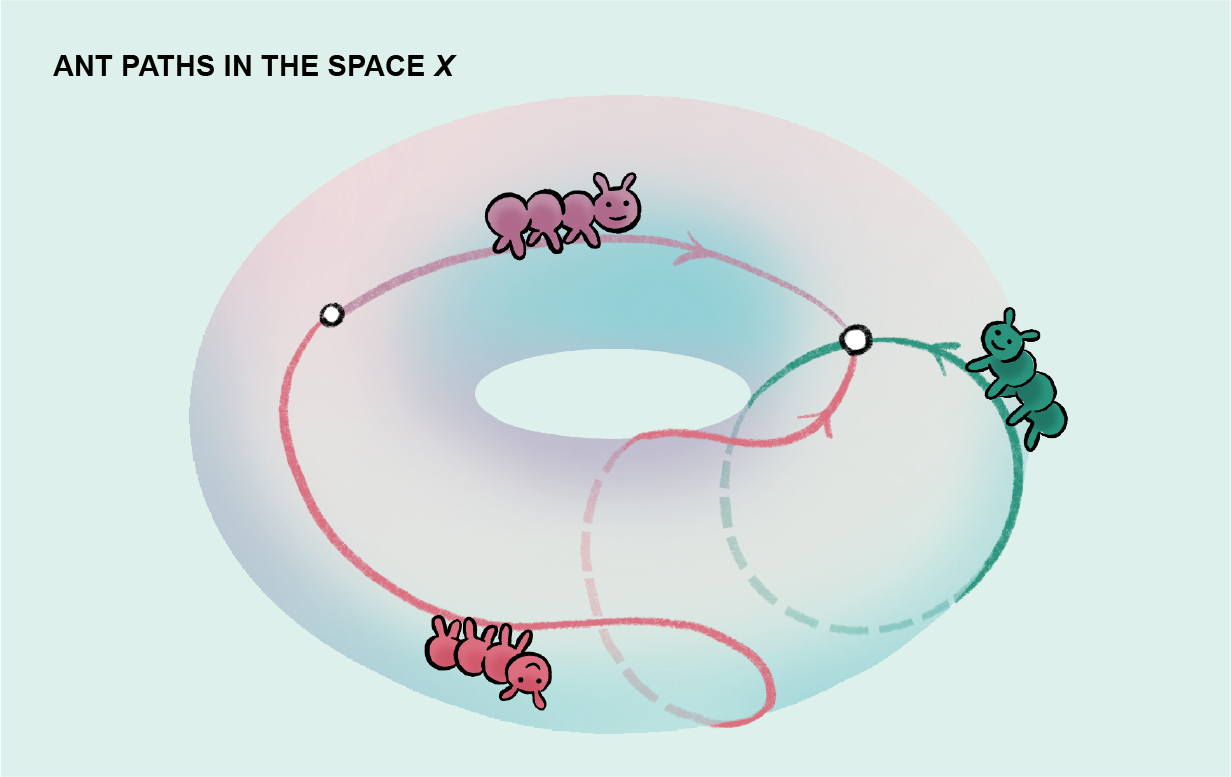
\includegraphics[width=1\linewidth]{7}
		\caption{\small\textit{\color{duongvaotoanhoc}Các phép đối xứng trên tấm thảm.}}
		\vspace*{-10pt}
	\end{figure}	
	Ưu thế then chốt của phỏng nhóm cơ bản là tính ``hàm tử'', nghĩa là mọi hàm liên tục $f: X \to Y$ giữa hai không gian tôpô cho ta một phép biến đổi $\pi_1 f: \pi_1 X \to \pi_1 Y$ giữa hai phỏng nhóm cơ bản. Phép biến đổi này tôn trọng phép hợp thành và đồng nhất của đường, nghĩa là $\pi_1(g \circ f) = \pi_1 g \circ \pi_1 f$ và $\pi_1(\pmb{1}_x) = \pmb{1}_{\pi_1 x}$. Hai tính chất này, gọi chung là ``tính hàm tử'', gợi ý rằng phỏng nhóm cơ bản giữ được những tính chất cốt lõi của không gian tôpô. Nói riêng, nếu hai không gian không tương đương đồng luân thì phỏng nhóm cơ bản của chúng cũng không tương đương.
	\vskip 0.1cm
	Dù vậy, phỏng nhóm cơ bản chưa phải là một bất biến hoàn chỉnh. Có thể dễ dàng phân biệt một đường tròn với hình tròn đặc mà đường tròn ấy bao quanh. Trong phỏng nhóm cơ bản của đường tròn, các đường giữa hai điểm cho trước, sai khác biến dạng liên tục (đồng luân), được gán với các số nguyên, chỉ số vòng mà đường này quay quanh đường tròn, với dấu $+$ hoặc $-$ chỉ chiều thuận hoặc ngược kim đồng hồ. Ngược lại, trong phỏng nhóm cơ bản của hình tròn, chỉ có duy nhất (sai khác đồng luân) một đường giữa bất kỳ cặp điểm nào. Phỏng nhóm cơ bản của phần bề mặt của quả bóng, hay một mặt cầu theo ngôn ngữ tôpô, cũng thỏa mãn chính chất này: tồn tại duy nhất, sai khác đồng luân, một đường giữa hai điểm bất kỳ.
	\begin{figure}[H]
		\centering
		\vspace*{-5pt}
		\captionsetup{labelformat= empty, justification=centering}
		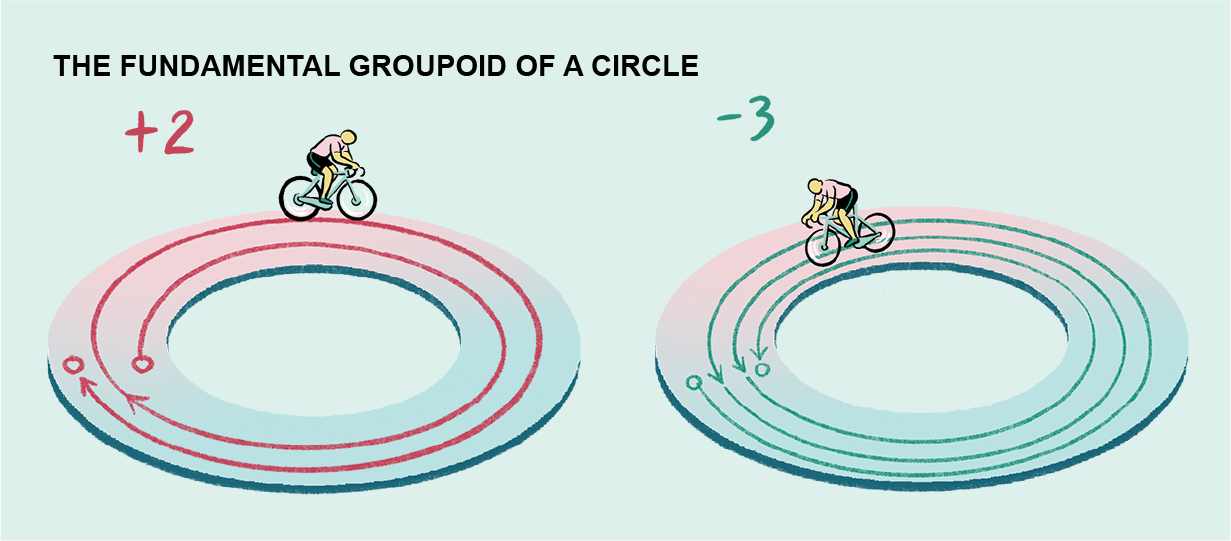
\includegraphics[width=1\linewidth]{8}
		\caption{\small\textit{\color{duongvaotoanhoc}Phỏng nhóm cơ bản của đường tròn.}}
		\vspace*{-10pt}
	\end{figure}
	Vấn đề lớn với phỏng nhóm cơ bản là điểm và đường không phát hiện được cấu trúc ở chiều cao hơn của không gian, vì bản thân điểm và đoạn lần lượt là $0$--chiều và $1$--chiều. Một giải pháp là xét thêm cả các hàm liên tục từ hình tròn $2$--chiều, được gọi là các phép đồng luân, cùng với các ``đồng luân bậc cao'', được định nghĩa là các hàm liên tục hình hình cầu đặc $3$--chiều và tương tự với các hình siêu cầu $4$--, $5$--, $6$--chiều hoặc hơn.
	\vskip 0.1cm
	Một câu hỏi tự nhiên là các điểm, đường, đồng luân và đồng luân bậc cao của một không gian $X$ thì tạo ra cấu trúc gì: cấu trúc $\pi_\infty$ này, gọi là $\infty$--phỏng nhóm cơ bản của X, định nghĩa một $\infty$--phạm trù, phiên bản vô hạn chiều của phạm trù đưa ra bởi Eilenberg và Mac Lane. Giống như phạm trù thông thường, một $\infty$--phạm trù gồm các vật và các phép biến đổi được vẽ như những mũi tên $1$--chiều, nhưng nó còn có thêm các phép ``biến đổi bậc cao'', được vẽ như các mũi tên $2$--chiều, mũi tên $3$--chiều, và cứ như vậy. Ví dụ, trong $\pi_\infty X$, các vật và các mũi tên lần lượt là các điểm và các đường -- lúc này ta không xét sai khác đồng luân nữa -- trong khi các biến đổi bậc cao lưu giữ thông tin đồng luân bậc cao. Cũng như trong phạm trù thông thường, các mũi tên (với số chiều cố định) có thể hợp thành: nếu ta có hai mũi tên $f: X \to Y$ và $g: Y \to Z$, ta phải có mũi tên thứ ba $g \circ f: X \to Z$. Nhưng cái khó ở đây là: để mô tả được những ví dụ rất tự nhiên như $\infty$--phỏng nhóm cơ bản của một không gian, luật hợp thành phải bị làm yếu đi. Với mỗi cặp mũi tên khả hợp thành, một mũi tên hợp thành tồn tại, nhưng nó không còn là duy nhất nữa.
	\begin{figure}[H]
		\centering
		\vspace*{-5pt}
		\captionsetup{labelformat= empty, justification=centering}
		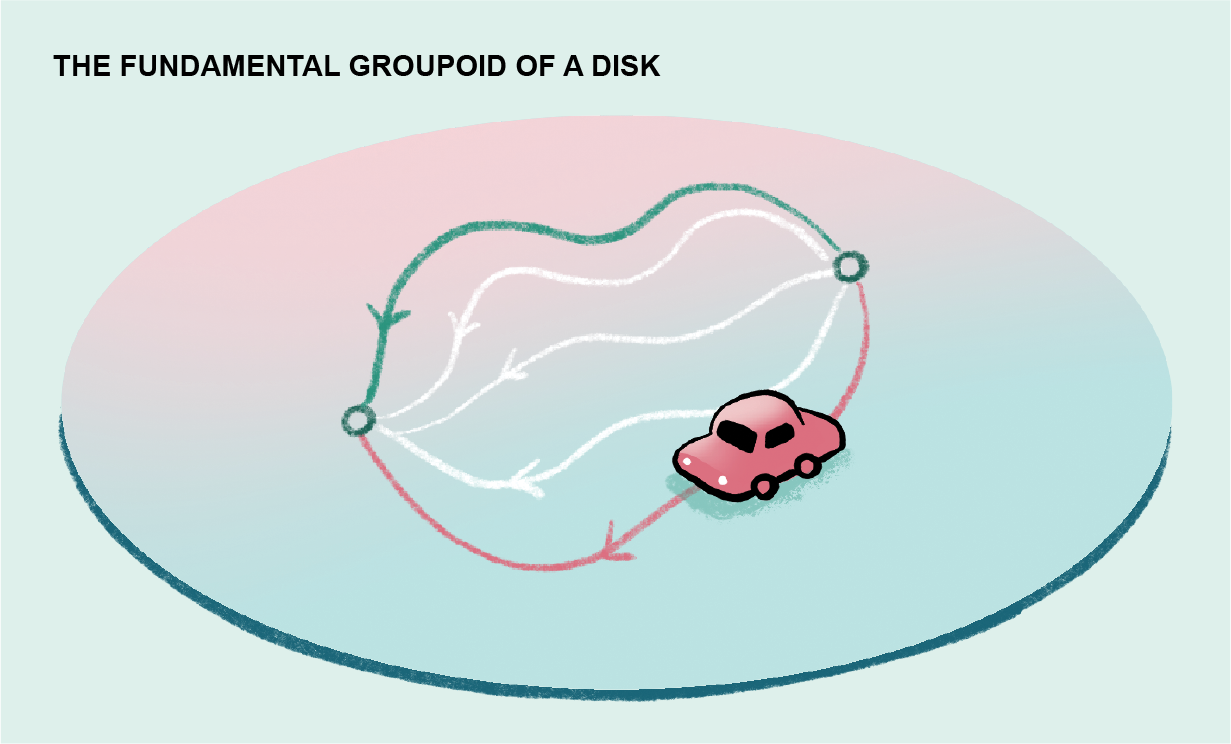
\includegraphics[width=1\linewidth]{9}
		\caption{\small\textit{\color{duongvaotoanhoc}Phỏng nhóm cơ bản của hình tròn.}}
		\vspace*{-10pt}
	\end{figure}
	Sự thiếu sót của tính duy nhất này thách thức việc định nghĩa $\infty$--phạm trù bằng cơ sở toán học bởi lý thuyết tập hợp cổ điển, vì ta không thể xem phép hợp thành như một phép toán như trong đại số phổ dụng nữa. Dù $\infty$--phạm trù đang dần trở thành đối tượng trung tâm của nghiên cứu hiện đại trong nhiều lĩnh tực toán học từ lý thuyết trường lượng tử tôpô đến hình học đại số hay tôpô đại số, chúng thường được xem là ``quá khó'' cho mọi người ngoài các chuyên gia, và nó không xuất hiện thường xuyên trong chương trình học, ngay cả sau đại học. Dù vậy, tôi và nhiều người khác xem $\infty$--phạm trù như một hướng đi mới và cách mạng, cho phép các nhà toán học mơ đến những liên kết mới mà không thể phát biểu và chứng minh một cách chặt chẽ bằng cách khác.
	\vskip 0.1cm
	\centerline{\bf\color{duongvaotoanhoc}Một số thuật ngữ Toán học hiện đại}
	\vskip 0.1cm
	$\bullet$ Hợp thành: chỉ việc áp dụng một phép biến đổi lên kết quả của một phép biến đổi khác.
	\vskip 0.1cm	
	$\bullet$ Phạm trù: một họ cụ thể gồm các vật và phép biến đổi giữa chúng, cùng một luật hợp thành.
	\vskip 0.1cm	
	$\bullet$ Đồng nhất: phép biến đổi từ một vật vào chính nó mà hoàn toàn không thay đổi vật đó.
	\vskip 0.1cm			
	$\bullet$ Đối xứng: một phép biến đổi khả nghịch từ một vật vào chính nó.
	\vskip 0.1cm	
	$\bullet$ Đẳng cấu: khái niệm ``như nhau'' về mặt cấu trúc, tồn tại giữa các cặp vật trong một phạm trù.
	\vskip 0.1cm
	$\bullet$ Phỏng nhóm cơ bản: phạm trù mà vật là điểm trong một không gian và các phép biến đổi là các đường sai khác đồng luân giữa chúng.
	\vskip 0.1cm		
	$\bullet$ Đồng luân: ``đường giữa hai đường", được định nghĩa là một biến dạng liên tục từ đường này thành đường kia.
	\vskip 0.1cm		
	$\bullet$ Phạm trù vô cực: phiên bản vô hạn chiều của phạm trù, nơi có thêm các biến đổi bậc cao và luật hợp thành bị làm yếu đi.
	\vskip 0.1cm	
	$\bullet$ Phỏng nhóm vô cực cơ bản: phạm trù vô cực gồm các điểm, đường, đồng luân và đồng luân bậc cao của một không gian.
	\vskip 0.1cm
	\textbf{\color{duongvaotoanhoc}Chân trời tương lai}
	\vskip 0.1cm
	Dẫu vậy, kinh nghiệm lịch sử cho thấy rằng phần lớn những kiến thức toán học mới lạ nhất hôm nay sẽ dần trở nên đủ dễ để dạy cho sinh viên toán ngài mai. Sẽ rất vui khi được quan sát, với tư cách là một người nghiên cứu $\infty$--phạm trù, cách mà nó có thể được đơn giản hóa đi. Chẳng hạn như một mẹo nhỏ về ngôn ngữ -- một phiên bản siêu cấp của từ ``the'' trong phạm trù -- có thể khiến cho sinh viên ở cuối thế kỷ XXI hiểu $\infty$--phạm trù một cách dễ dàng như phạm trù thông thường ngày nay. Tiên đề then chốt của lý thuyết phạm trù thông thường là sự tồn tại duy nhất của một phép biến đổi hợp thành $g \circ f: X \to Z$ với mỗi cặp biến đổi $f: X \to Y$ và $g: Y \to Z$, được chọn ra từ tập các phép biến đổi từ $X$ vào $Z$. Trái lại, trong một $\infty$--phạm trù, có một không gian các mũi tên từ $X$ vào $Z$, thứ mà trong $\infty$--phỏng nhóm cơ bản có thể hiểu là ``không gian đường''. Phiên bản đúng của tính hợp thành duy nhất trong phạm trù thông thường là mệnh đề: trong một $\infty$--phạm trù, không gian các hợp thành là ``co rút được'', nghĩa là mỗi điểm của nó đều có thể suy sụp một cách liên tục qua một vụ nổ ``Big Bang ngược'' về một điểm gốc duy nhất.
	\vskip 0.1cm
	Chú ý rằng tính co rút được không suy ra rằng có duy nhất một hợp thành: thật vậy, ta đã thấy rằng trong $\infty$--phỏng nhóm cơ bản, có thể có rất nhiều đường hợp thành. Nhưng tính co rút được đảm bảo rằng hai đường hợp thành luôn đồng luân, và hai phép đồng luân bất kỳ giữa hai đường hợp thành luôn liên kết với nhau bởi một đồng luân bậc cao, và cứ như vậy.
	\begin{figure}[H]
		\centering
		\vspace*{-5pt}
		\captionsetup{labelformat= empty, justification=centering}
		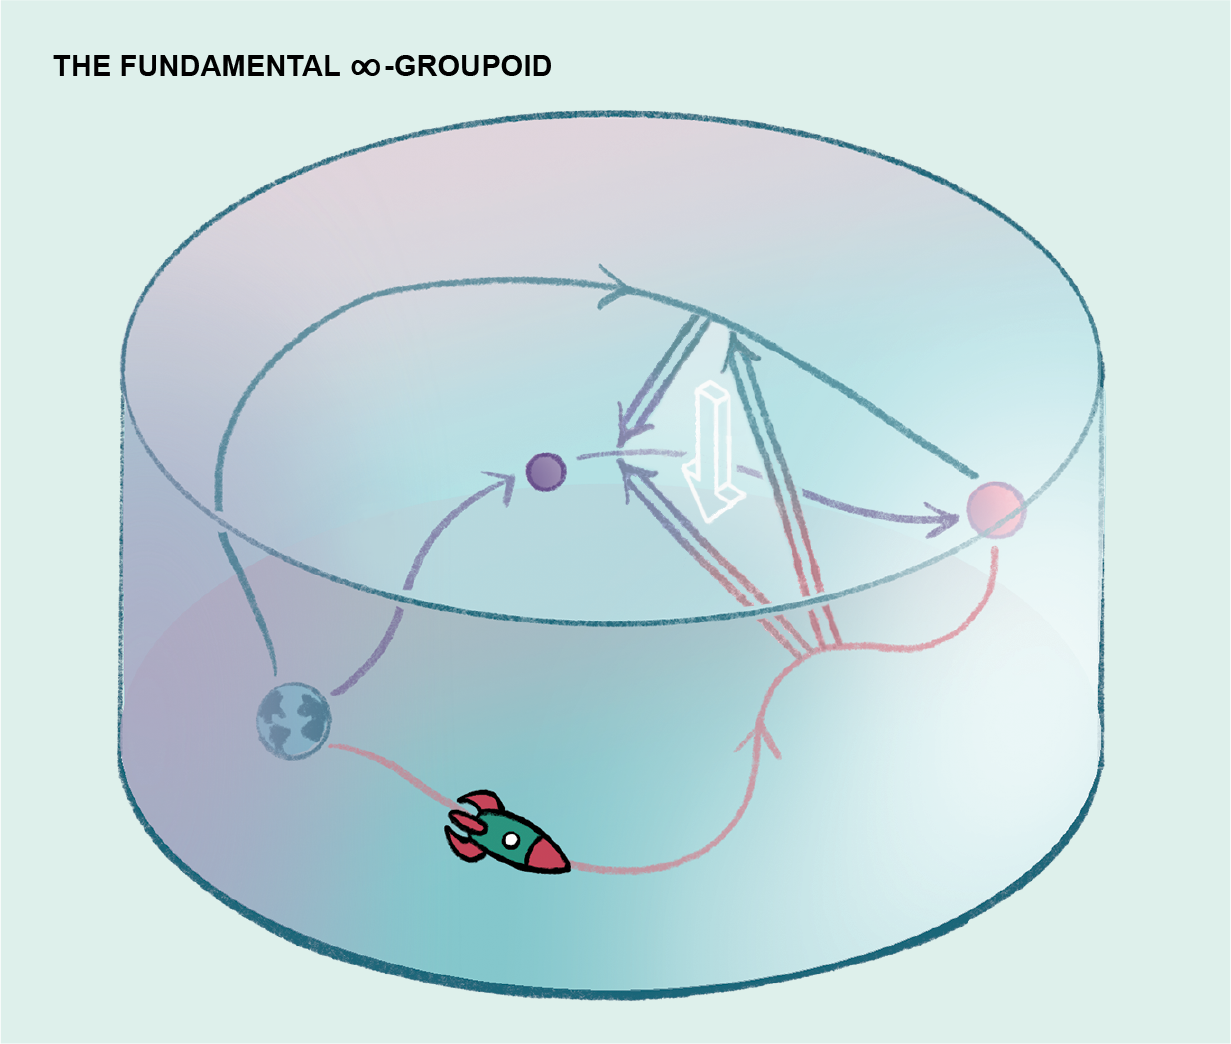
\includegraphics[width=1\linewidth]{10}
		\caption{\small\textit{\color{duongvaotoanhoc}Phỏng nhóm vô cực cơ bản.}}
		\vspace*{-10pt}
	\end{figure}
	Ý tưởng về sự duy nhất như điều kiện co rút được này là một ý tưởng trung tâm trong hệ cơ sở toán học mới được đề xuất bởi Vladimir Voedvodsky và nhiều người khác. Các nhà toán học khắp nơi đang hợp sức phát triển những ``phụ tá chứng minh'' bằng máy tính có khả năng kiểm tra từng dòng một trong chứng minh hình thức của một kết quả toán học. Những phụ tá này có một cơ chế bắt chước theo một kỹ thuật chung trong toán học là chuyển thông tin từ một vật sang một vật khác được coi là giống vật ban đầu qua một đẳng cấu tường minh hoặc một tương đương đồng luân. Cơ chế này cho phép người dùng chuyển một chứng minh liên quan đến một điểm trong không gian qua một đường nối nó đến một điểm khác, đưa ra một định nghĩa chặt chẽ về khái niệm ``như nhau'' của tôpô.
	\vskip 0.1cm
	Trong một tham luận năm $1974$, nhà toán học Micheal Atiyah đã viết ``Mục tiêu thực sự của lý thuyết là tổ chức lại một cách có hệ thống kinh nghiệm quá khứ sao cho thế hệ sau, học sinh của chúng ta, rồi học sinh của họ, rồi sau đó nữa, có thể tiếp thu những khía cạnh cốt lõi mà ít tốn sức nhất, và đó là cách duy nhất mà bạn có thể liên tục tích lũy và xây dựng bất kỳ hoạt động khoa học nào mà không đi đến ngõ cụt.'' Lý thuyết phạm trù đóng vai trò này trong toán học hiện đại: nếu toán học là khoa học của sự tương tự, các khuôn mẫu, thì lý thuyết phạm trù là khoa học của các khuôn mẫu tư duy toán học -- ``toán học của toán học'', như Eugenia Cheng (Viện Nghệ thuật Chicago), đã gọi.
	\vskip 0.1cm
	Lý do ta dạy được rất nhiều trong một môn toán ở đại học ngày nay là vì hiểu biết của chúng ta về rất nhiều khái niệm toán học khác nhau đã được đơn giản hóa nhờ sự trừu tượng, có thể xem như lùi khỏi bài toán cụ thể để quan sát tổng quan toán học. Rất nhiều chi tiết sẽ ẩn đi ở tầm này -- xấp xỉ số chẳng hạn, hoặc bất kỳ thứ gì liên quan đến số -- nhưng một sự thật đáng chú ý là nhiều định lý trong đại số, lý thuyết tập hợp, tôpô và hình học đại số thường đúng vì cùng một lý do đằng sau, và khi đó, các chứng minh được diễn tả bằng ngôn ngữ phạm trù.
	\vskip 0.1cm
	Có gì ở chân trời tương lai? Đang hình thành một sự đồng thuận trong nhiều lĩnh vực toán học rằng các đối tượng cơ bản của toán học thế kỷ XXI là các $\infty$--phạm trù, giống như ở thế kỷ XX là các phạm trù thông thường. Ta hi vọng rằng chiếc tháp vô hạn của các mũi tên ở mọi chiều này, thứ cần nghiên cứu tỷ mỉ trong $\infty$--phạm trù, đến lúc nào đó sẽ thu gọn về về tiềm thức chung của toán học, với các không gian co rút được suy sụp về một điểm duy nhất. Và ta có thể tự hỏi: Nếu những tiến bộ này xuất hiện ở thế kỷ XX, toán ở học ở cuối thế kỷ XXI sẽ đi về đâu?
\end{multicols} 
	\newpage
%	
%	\thispagestyle{empty}
%	\begingroup 
%	\AddToShipoutPicture*{\put(20,25){\includegraphics[width=18cm]{hoangtuy}}}
%	\centering
%	\vspace*{0cm}
%	\endgroup
%	\newpage	
%	\pagestyle{empty}
%	
%	\setcounter{figure}{0}
%	\thispagestyle{quantoannone}
\pagestyle{quantoan}
\everymath{\color{quantoan}}
\graphicspath{{../quantoan/pic/}}
\blfootnote{\color{quantoan}\color{quantoan}$^1$Viện Toán học.}
\begingroup
\AddToShipoutPicture*{\put(0,616){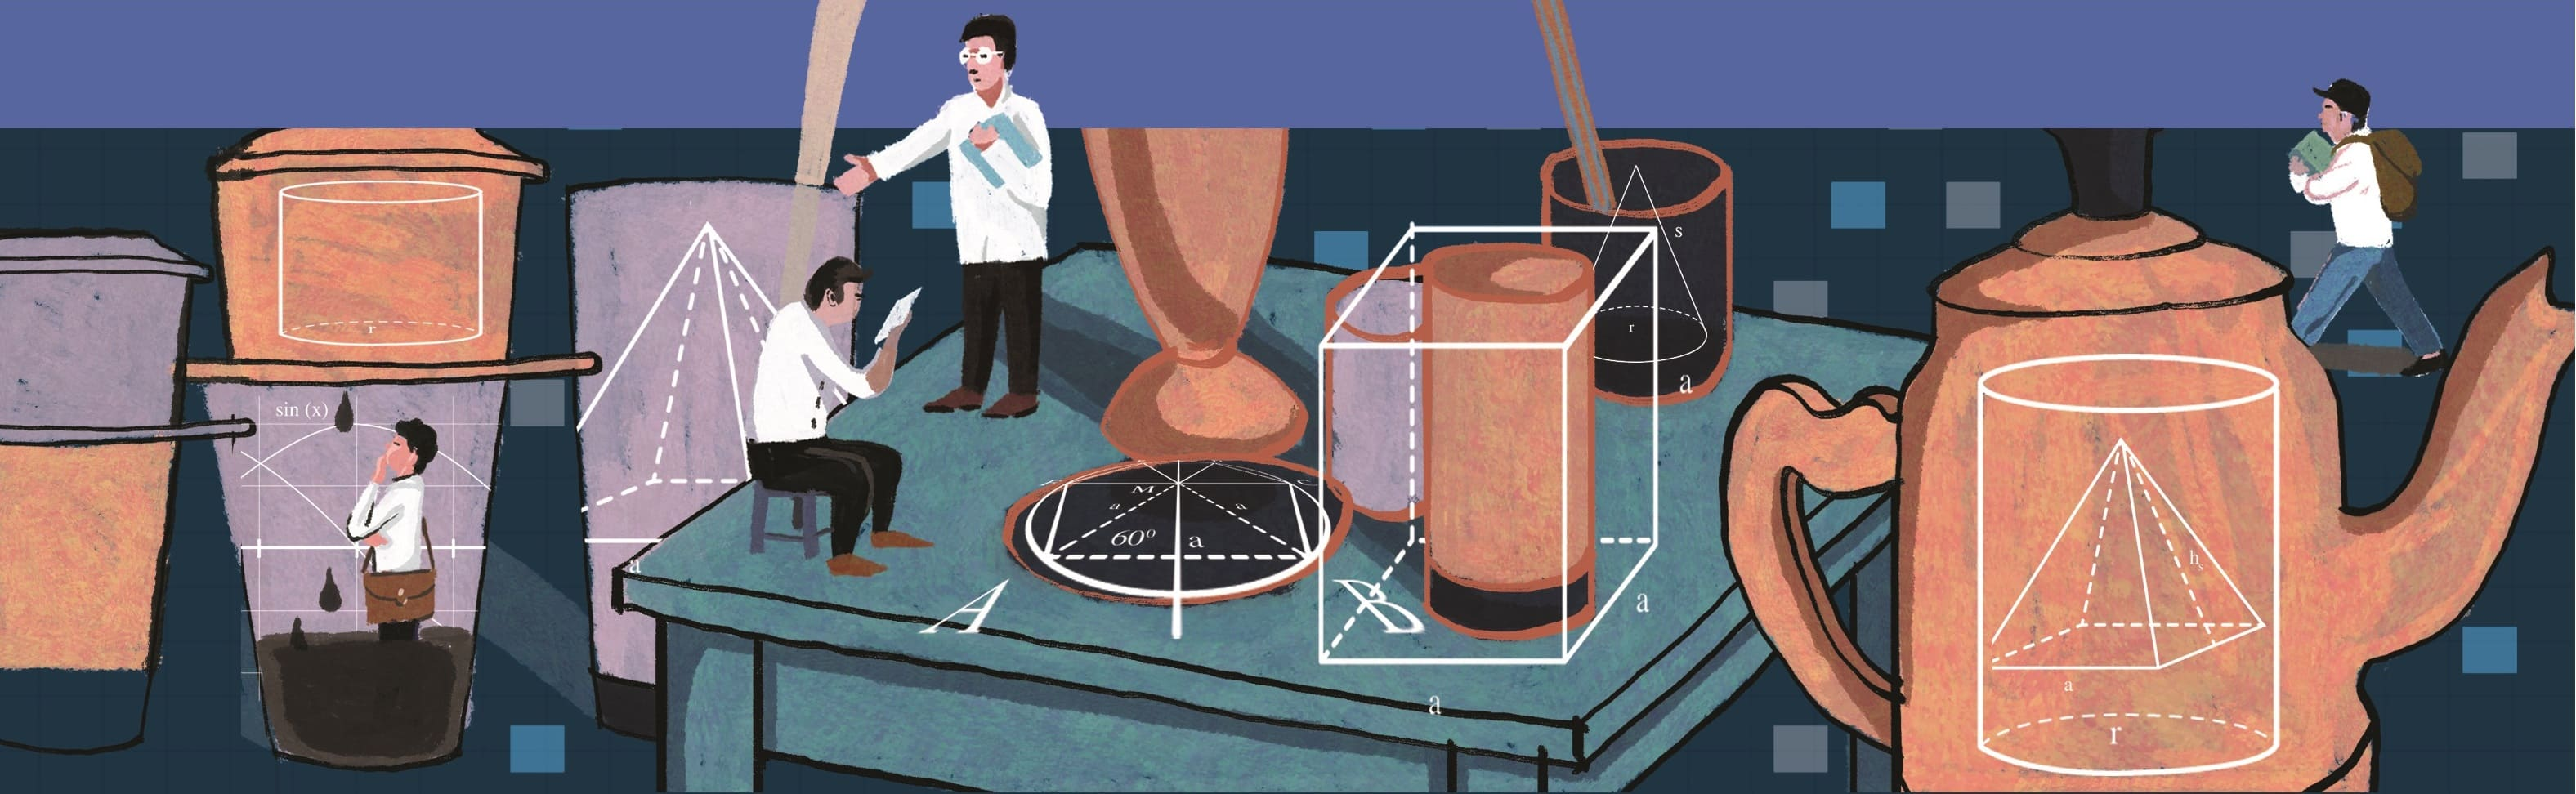
\includegraphics[width=19.3cm]{../bannerquantoan}}}
\AddToShipoutPicture*{\put(156,550){
\includegraphics[scale=1]{../tieude3.pdf}}}
\centering
\endgroup

\vspace*{160pt}

\begin{multicols}{2}	
	Ngày nay số âm đã được học sinh làm quen từ lớp $6$. Nhưng nhân loại đã mất tới $2000$ năm để có thể chấp nhận được nó như cách mà học sinh lớp $6$ ngày nay chấp nhận. 
	\begin{figure}[H]
		\vspace*{-5pt}
		\centering
		\captionsetup{labelformat= empty, justification=centering}
		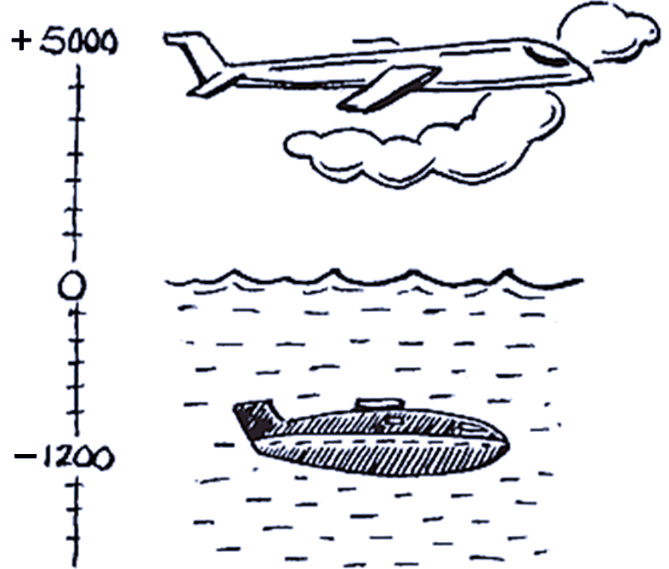
\includegraphics[width= 1\linewidth]{1}
%		\caption{\small\textit{\color{}}}
		\vspace*{-10pt}
	\end{figure}
	Nhìn lại lịch sử cho chúng ta thấy sự vật lộn trong quá trình trừu tượng hóa của Toán học. Hy vọng, theo dõi quá trình vất vả này, các thầy cô giáo THCS sẽ có thêm sự cảm thông đối với những học sinh ``dốt toán". Biết đâu, các em có thể không dốt mà chỉ đang vật lộn với việc phản biện như những nhà toán học kiệt xuất đã từng phản biện về số âm? 
	\vskip 0.1cm
	-- Thế kỷ V TCN, Hy Lạp: Trường phái Pythagoras coi số là ``nhiều đơn vị". Vì vậy với họ ``một" không phải là một số. Không có dấu hiệu nào về số âm trong các ghi chép của họ.
	\vskip 0.1cm
	-- Thế kỷ IV TCN, Hy Lạp: Aristotle đã đưa ra sự phân biệt giữa số (tức là số tự nhiên) và độ lớn (``số đó chia hết thành các số chia mà có thể chia vô hạn"), nhưng không đưa ra dấu hiệu nào về khái niệm số âm hoặc độ lớn âm.
	\vskip 0.1cm
	-- Khoảng năm $300$ TCN, Hy Lạp: Các tập VII, VIII và IX trong cuốn \textit{Cơ sở} của Euclid liên quan đến lý thuyết cơ bản về số. Euclid tiếp tục sự phân biệt của Aristotle giữa số và độ lớn, nhưng vẫn không có dấu hiệu nào về số âm.
	\vskip 0.1cm
	-- Thế kỷ I TCN -- thế kỷ I, Trung Quốc: Trong \textit{Cửu chương Toán thuật}, số âm đã được sử dụng trong chương về giải hệ phương trình. Các que màu đỏ được sử dụng để biểu thị các hệ số dương, màu đen để biểu thị các hệ số âm. Các quy tắc cho số có dấu đã được đưa ra.
	\vskip 0.1cm
	-- Thế kỷ III, Hy Lạp: Dấu hiệu đầu tiên về số âm trong một tác phẩm phương Tây xuất hiện trong cuốn \textit{Số học} của Diophantus, trong đó ông gọi phương trình mà trong ký hiệu hiện đại sẽ được biểu thị bởi $4x + 20 = 0$ là ``vô lý", vì nó sẽ cho nghiệm $x=-5$. Ông cũng nói, ``một số bị trừ, nhân với một số bị trừ, cho một số được cộng (thêm vào)". Vì vậy ông có thể xử lý các biểu thức chẳng hạn như $(x-1)(x-2)$, trong ký hiệu hiện đại. Tuy nhiên, có thể tìm thấy những chỉ dẫn trong tác phẩm của Diophantus rằng ông không có khái niệm trừu tượng về số âm.
	\vskip 0.1cm
	-- Thế kỷ VII, Ấn Độ: Số âm được sử dụng để biểu thị các khoản nợ trong khi số dương biểu thị tài sản. Nhà toán học và thiên văn học Brahmagupta đã sử dụng các số âm để thống nhất phương pháp xử lý phương trình bậc hai của Diophantus từ ba trường hợp thành một trường hợp duy nhất mà chúng ta quen thuộc ngày nay.
	\vskip 0.1cm
	-- Thế kỷ IX, Trung Đông: Mặc dù người Ả Rập đã quen thuộc với các số âm từ công trình của các nhà toán học Ấn Độ, nhưng họ bác bỏ chúng. Cuốn sách \textit{al--Kitāb al--Mukhtaṣar fī Ḥisāb al--Jabr wal--Muqābalah} (mà từ đó chúng ta có thuật ngữ ``algebra" -- đại số) của Muhammad ibn Musa al--Khwarizmi không sử dụng số âm hoặc hệ số âm.
	\vskip 0.1cm
	-- Thế kỷ XIII, Trung Quốc: Các số âm được biểu thị bằng cách vẽ một nét chéo qua chữ số khác không ngoài cùng bên phải của số đó.
	\vskip 0.1cm
	-- Thế kỷ XIII, Châu Âu: Fibonacci không đề cập đến số âm trong cuốn sách \textit{Liber Abaci} của mình, nhưng trong cuốn \textit{Flos} sau đó, ông giải thích nghiệm âm như là sự thua lỗ.
	\vskip 0.1cm
	-- Thế kỷ XV, Châu Âu: Chuquet là người đầu tiên sử dụng số âm trong một tác phẩm ở Châu Âu.
	\vskip 0.1cm
	-- Thế kỷ XVI, Châu Âu: 
	\vskip 0.1cm
	$\circ$ Cardan (Cardano), trong cuốn sách \textit{Ars Magna} của mình đã đưa vào các nghiệm âm của các phương trình và nêu các quy luật cơ bản của hoạt động với các số âm. Ông gọi các số dương là thực và các số âm là hư cấu.
	\vskip 0.1cm
	$\circ$ Viete không thừa nhận số âm.
	\vskip 0.1cm
	-- Thế kỷ XVII, Châu Âu:
	\vskip 0.1cm
	$\circ$ Descartes chấp nhận một phần khái niệm số âm. Ông không công nhận nghiệm âm vì chúng đại diện cho các số ``nhỏ hơn không có gì". Tuy nhiên, ông đã chỉ ra rằng một phương trình có nghiệm âm có thể được biến đổi thành một phương trình có nghiệm dương, điều này khiến ông chấp nhận các số âm.
	\vskip 0.1cm
	$\circ$ Pascal coi phép ``trừ đi $4$ từ $0$" là điều hoàn toàn vô nghĩa.
	\vskip 0.1cm
	$\circ$ Nhà thần học và toán học Antoine Arnauld lập luận chống lại số âm bằng cách sử dụng tỷ lệ; nói rằng tỷ lệ $-1$ trên $1$ giống với tỷ lệ $1$ trên $-1$ là vô lý, vì ``Làm thế nào tỷ lệ giữa một anh nhỏ với một anh lớn hơn lại như giữa anh lớn hơn với anh nhỏ hơn?"
	\vskip 0.1cm
	-- Thế kỷ XVIII, Châu Âu:
	\vskip 0.1cm
	$\circ$ Leibniz đồng ý với lập luận của Arnaud đối với các số âm, nhưng nói rằng vì về hình thức các tỷ lệ như vậy là đúng, nên người ta vẫn có thể tính toán với chúng.
	\vskip 0.1cm
	$\circ$ Maclaurin đã xử lý các đại lượng âm ngang hàng với các đại lượng dương trong tác phẩm \textit{A Treatise of Algebra} của ông.
	\vskip 0.1cm 
	$\circ$ Euler mở đầu tác phẩm \textit{Nhập môn tổng quan về Đại số} với một thảo luận về các phép toán trên các đại lượng dương và âm. Ông sử dụng ví dụ về một khoản nợ để biện minh rằng một số âm lần số dương là một số âm.  
	\vskip 0.1cm
	-- Thế kỷ XIX, Châu Âu: Hamilton đã cố gắng đưa các số âm lên một nền tảng lý thuyết vững chắc (thay vì khái niệm về đại lượng ``nhỏ hơn không có gì") bằng cách sử dụng ý tưởng về ``thời gian thuần túy" xuất phát từ tác phẩm \textit{Phê bình lý tính thuần túy} của Kant. Nỗ lực này có vẻ khá kỳ lạ đối với chúng ta ngày nay, nhưng nó đã giúp ích trong việc phát triển các \textit{quaternion}, ví dụ đầu tiên về một hệ đại số không thỏa mãn tính giao hoán.
	\begin{flushright}
		Theo \url{https://web.ma.utexas.edu/users/mks/326K/Negnos.html}
	\end{flushright}
\end{multicols}
%	\newpage
%	
%	\setcounter{figure}{0}
%	\thispagestyle{toancuabinone}
\pagestyle{toancuabi}
\everymath{\color{toancuabi}}
%\blfootnote{$^1$\color{toancuabi}Đại học Thăng Long.}
\graphicspath{{../toancuabi/pic/}}
\begingroup
\AddToShipoutPicture*{\put(0,616){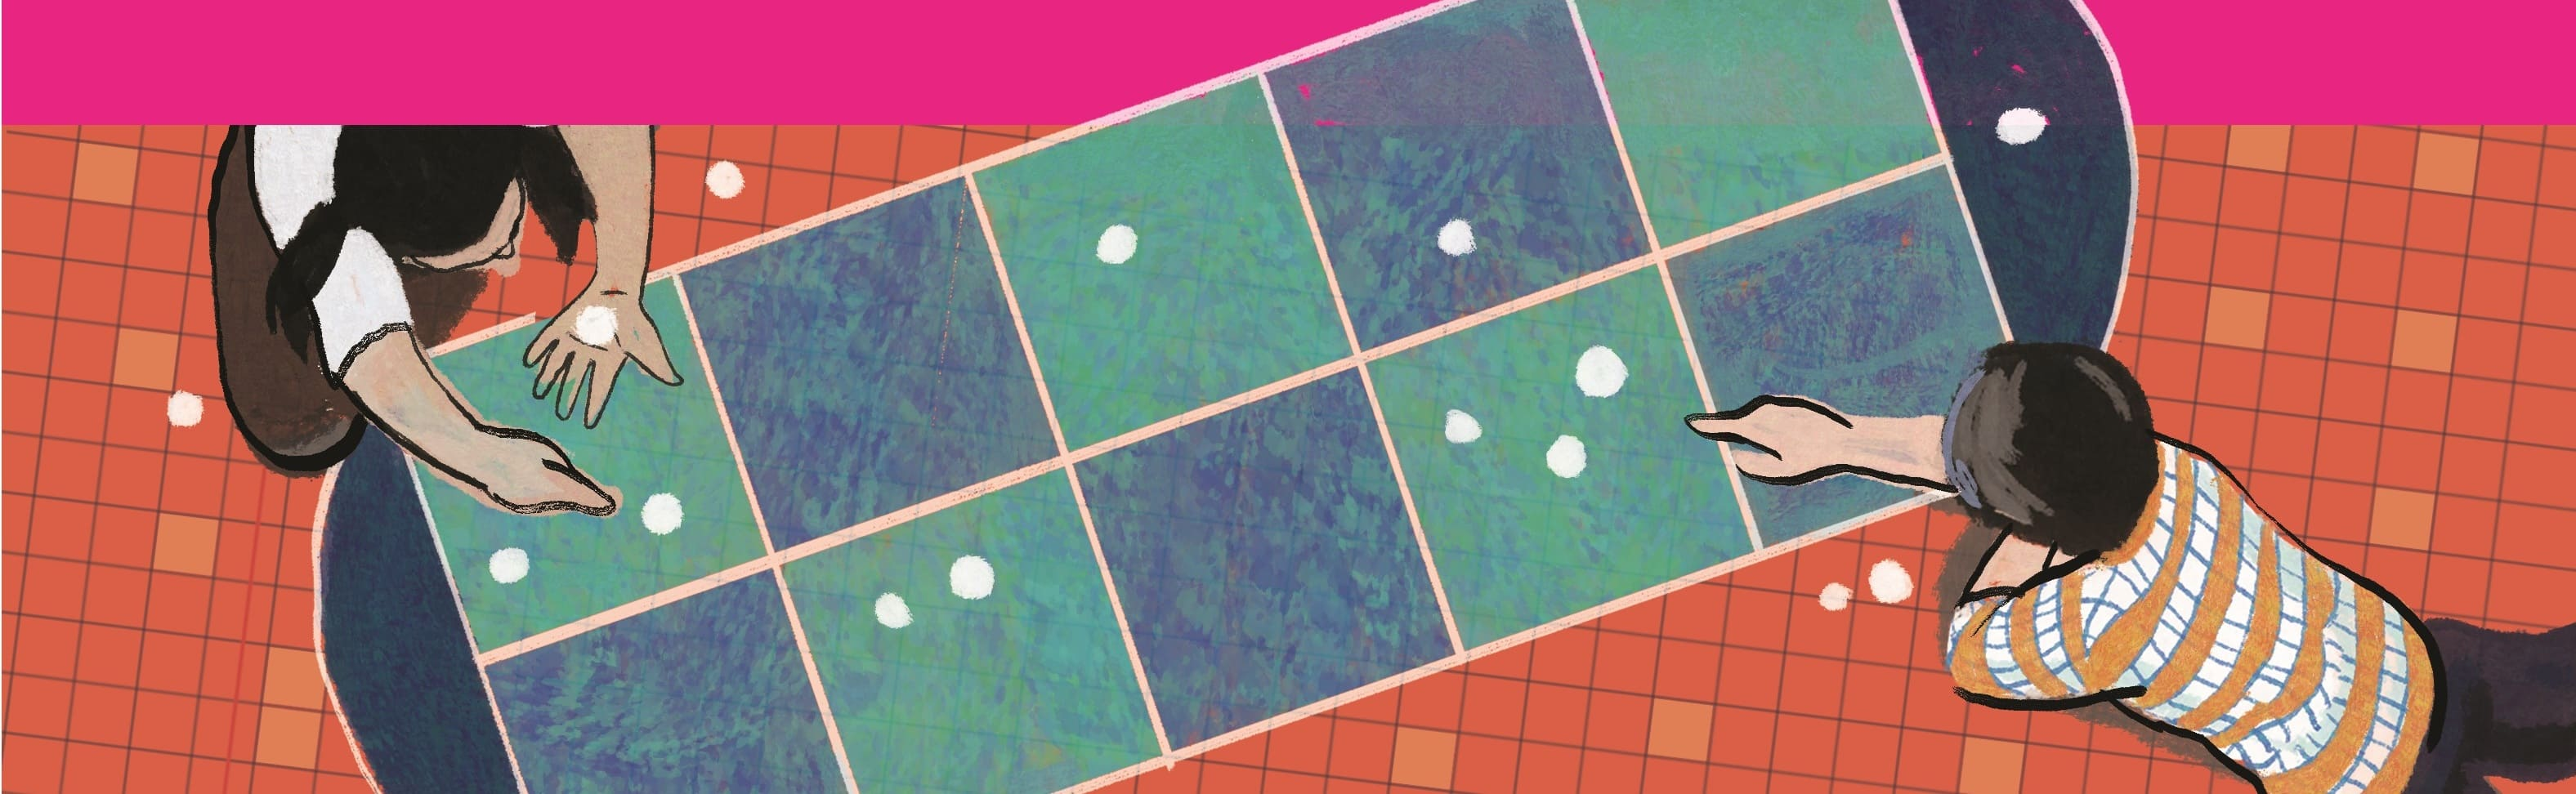
\includegraphics[width=19.3cm]{../bannertoancuabi}}}  
\AddToShipoutPicture*{\put(78,550){
\includegraphics[scale=1]{../tieude.pdf}}} 
\centering
\endgroup
\vspace*{160pt}

\begin{multicols}{2}
	Để điều tra một vụ án về kinh tế, Thám tử Xuân Phong cần thẩm vấn các đại diện của hai công ty vốn cạnh tranh kịch liệt với nhau là Sungsang và TungTeng. Qua thư ký bố trí xếp lịch, Xuân Phong mời được ba người là ông Kim, ông Lee và ông Han của hai công ty đình đám nọ tới văn phòng. Lịch sử cạnh tranh hàng chục năm nay của hai công ty này luôn chỉ ra rằng: các đại diện của cùng một công ty luôn nói thật với nhau, còn với đại diện của công ty cạnh tranh lại luôn \linebreak nói dối. 
	\vskip 0.1cm
	Các vị khách có mặt đúng giờ tại văn phòng thám tử  trong các bộ com--lê sang trọng xứng với đẳng cấp của đại diện cho các công ty hàng đầu về công nghệ. Vừa nhìn thấy  nhau, ông Kim đã  tiến tới trước mặt ông Lee và nói ``Tôi tới từ công ty Sungsang". Ông Lee trả lời ngay ``Ô thế à! Vậy là ông và ông Han cùng làm ở một công ty đấy!".
	\vskip 0.1cm
	Từ đoạn hội thoại trên, Xuân Phong xác định được ngay ông Han làm ở công ty nào. Em có thể lập luận xem làm cách nào mà thám tử lại biết vậy được không?
%	Lời giải
%	\vskip 0.1cm
%	Các em xét hai trường hợp sau đây: ông Kim và ông Lee làm ở cùng một công ty hoặc họ làm ở hai công ty khác nhau.
%	\vskip 0.1cm
%	Trường hợp đầu tiên, nếu ông Kim và ông Lee cùng làm ở một công ty, thì do họ nói thật với nhau, suy ra ông Kim làm ở công ty Sungsang. Nhưng vì ông Lee cũng nói thật, suy ra ông Han và ông Kim cùng làm ở công ty Sungsang.
%	\vskip 0.1cm
%	Trường hợp thứ hai, nếu họ làm khác công ty, thì ông Kim đã nói dối ông Lee, vì thế thực ra ông Kim làm ở công ty TungTeng. Nhưng do ông Lee cũng nói dối ông Kim, nên ông Kim và ông Han phải làm ở các công ty khác nhau. Vì ông Kim làm việc ở công ty TungTeng, nên ông Han làm việc ở công ty Sungsang.
%	\vskip 0.1cm
%	Như vậy, trong mọi trường hợp, ông Han luôn làm việc ở công ty Sungsang.
\end{multicols}
	\begin{figure}[H]
	\centering
	\vspace*{-5pt}
	\captionsetup{labelformat= empty, justification=centering}
	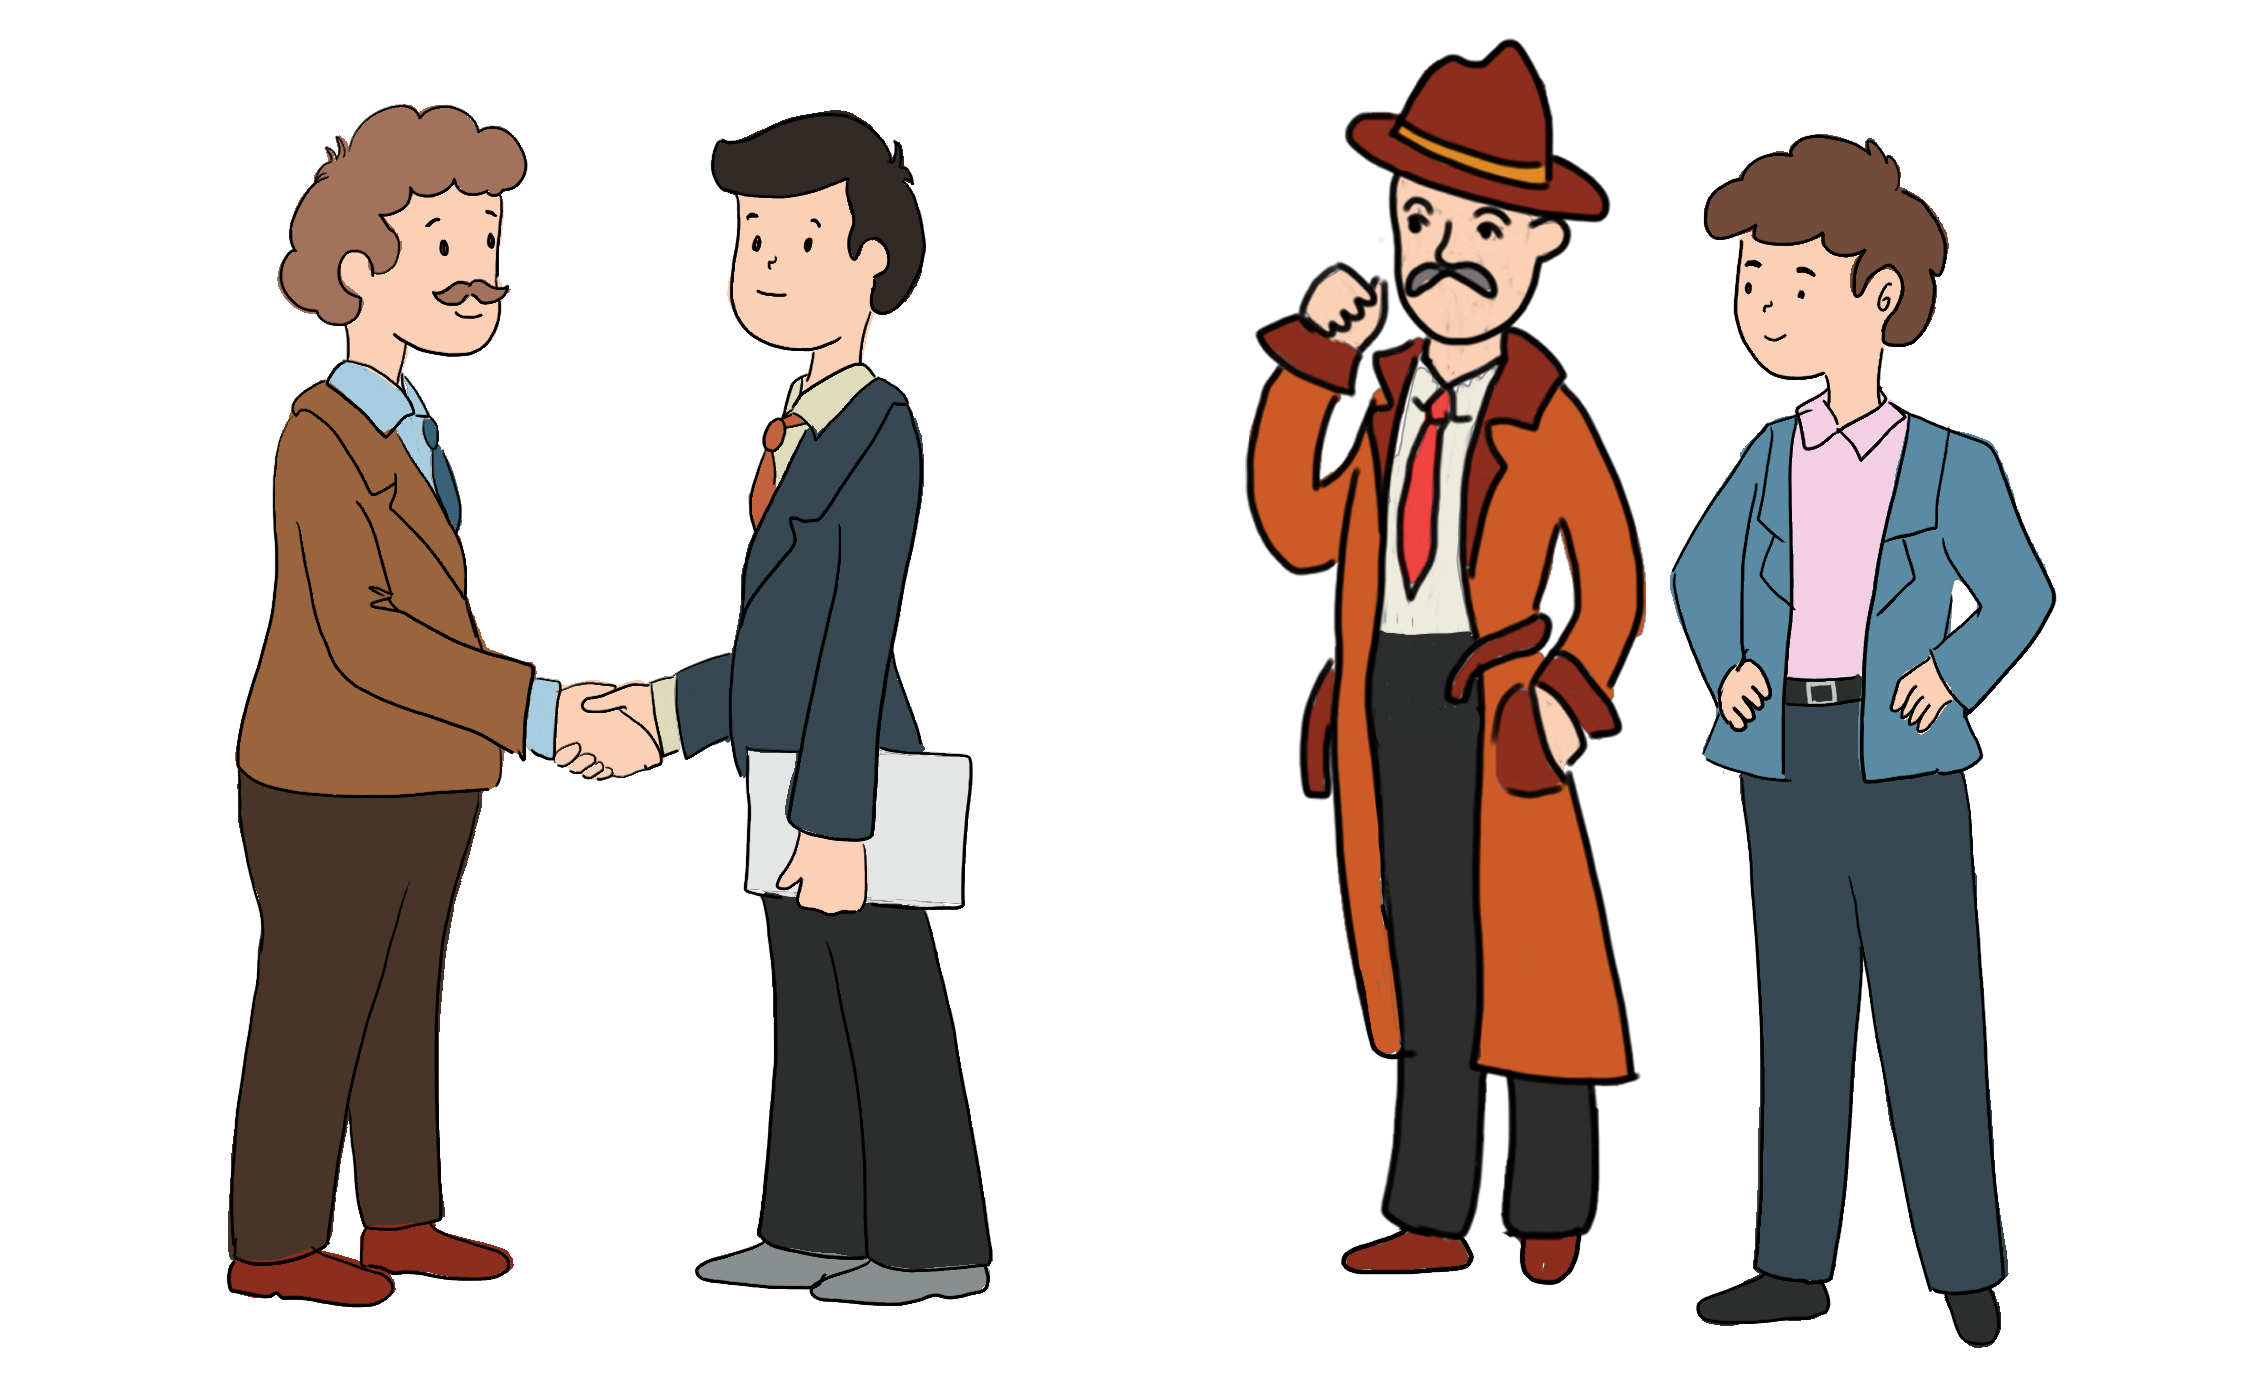
\includegraphics[width=1\linewidth]{xuanphong}
	\vspace*{-5pt}
	\end{figure}
\newpage
\begingroup
\AddToShipoutPicture*{\put(115,670){
\includegraphics[scale=1]{../tieude11.pdf}}} 
\centering
\endgroup
\vspace*{33pt}

\begin{multicols}{2}
	$\pmb{1.}$	Bạn Công đã trả $24$ nghìn đồng để mua được $1$ cuốn vở, $2$ chiếc bút chì và $1$ cái tẩy. Bạn Nam thì trả tận $54$ nghìn đồng để mua được $2$ cuốn vở, $3$ chiếc bút chì và $3$ cái tẩy. Hỏi bạn An đã trả bao nhiêu tiền để mua được $2$ cuốn vở, $5$ chiếc bút chì và $1$ cái tẩy?
	\begin{figure}[H]
		\centering
		\vspace*{-5pt}
		\captionsetup{labelformat= empty, justification=centering}
		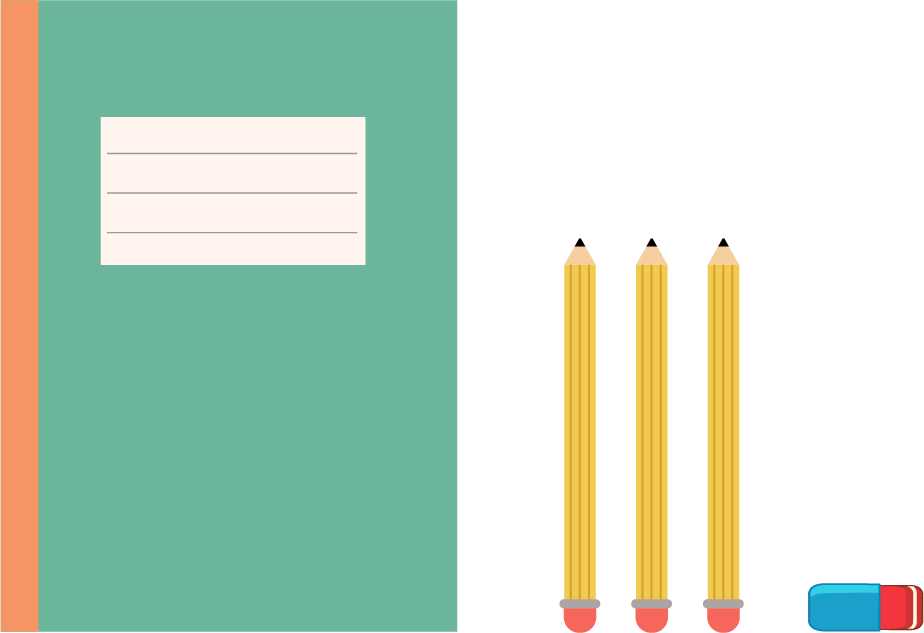
\includegraphics[width=1\linewidth]{Pi3_bai1}
		\vspace*{-10pt}
	\end{figure}
	$\pmb{2.}$ Bác Tuyết mang sữa đựng đầy trong hai chiếc thùng ra chợ bán. Lượng sữa trong thùng to nhiều gấp $3$ lần lượng sữa trong chiếc thùng nhỏ. Khi trong chiếc thùng nhỏ còn có $15$ lít sữa, còn thùng to còn $35$ lít sữa, bác Tuyết đổ dồn một lượng sữa từ thùng to cho đầy chiếc thùng nhỏ. Khi đó trong chiếc thùng to lượng sữa còn lại  đầy tới một nửa thùng. Hỏi bác Tuyết đã đổ bao nhiêu sữa từ thùng to sang thùng nhỏ, và dung tích của mỗi thùng là bao nhiêu?
	\begin{figure}[H]
		\centering
		\vspace*{-10pt}
		\captionsetup{labelformat= empty, justification=centering}
		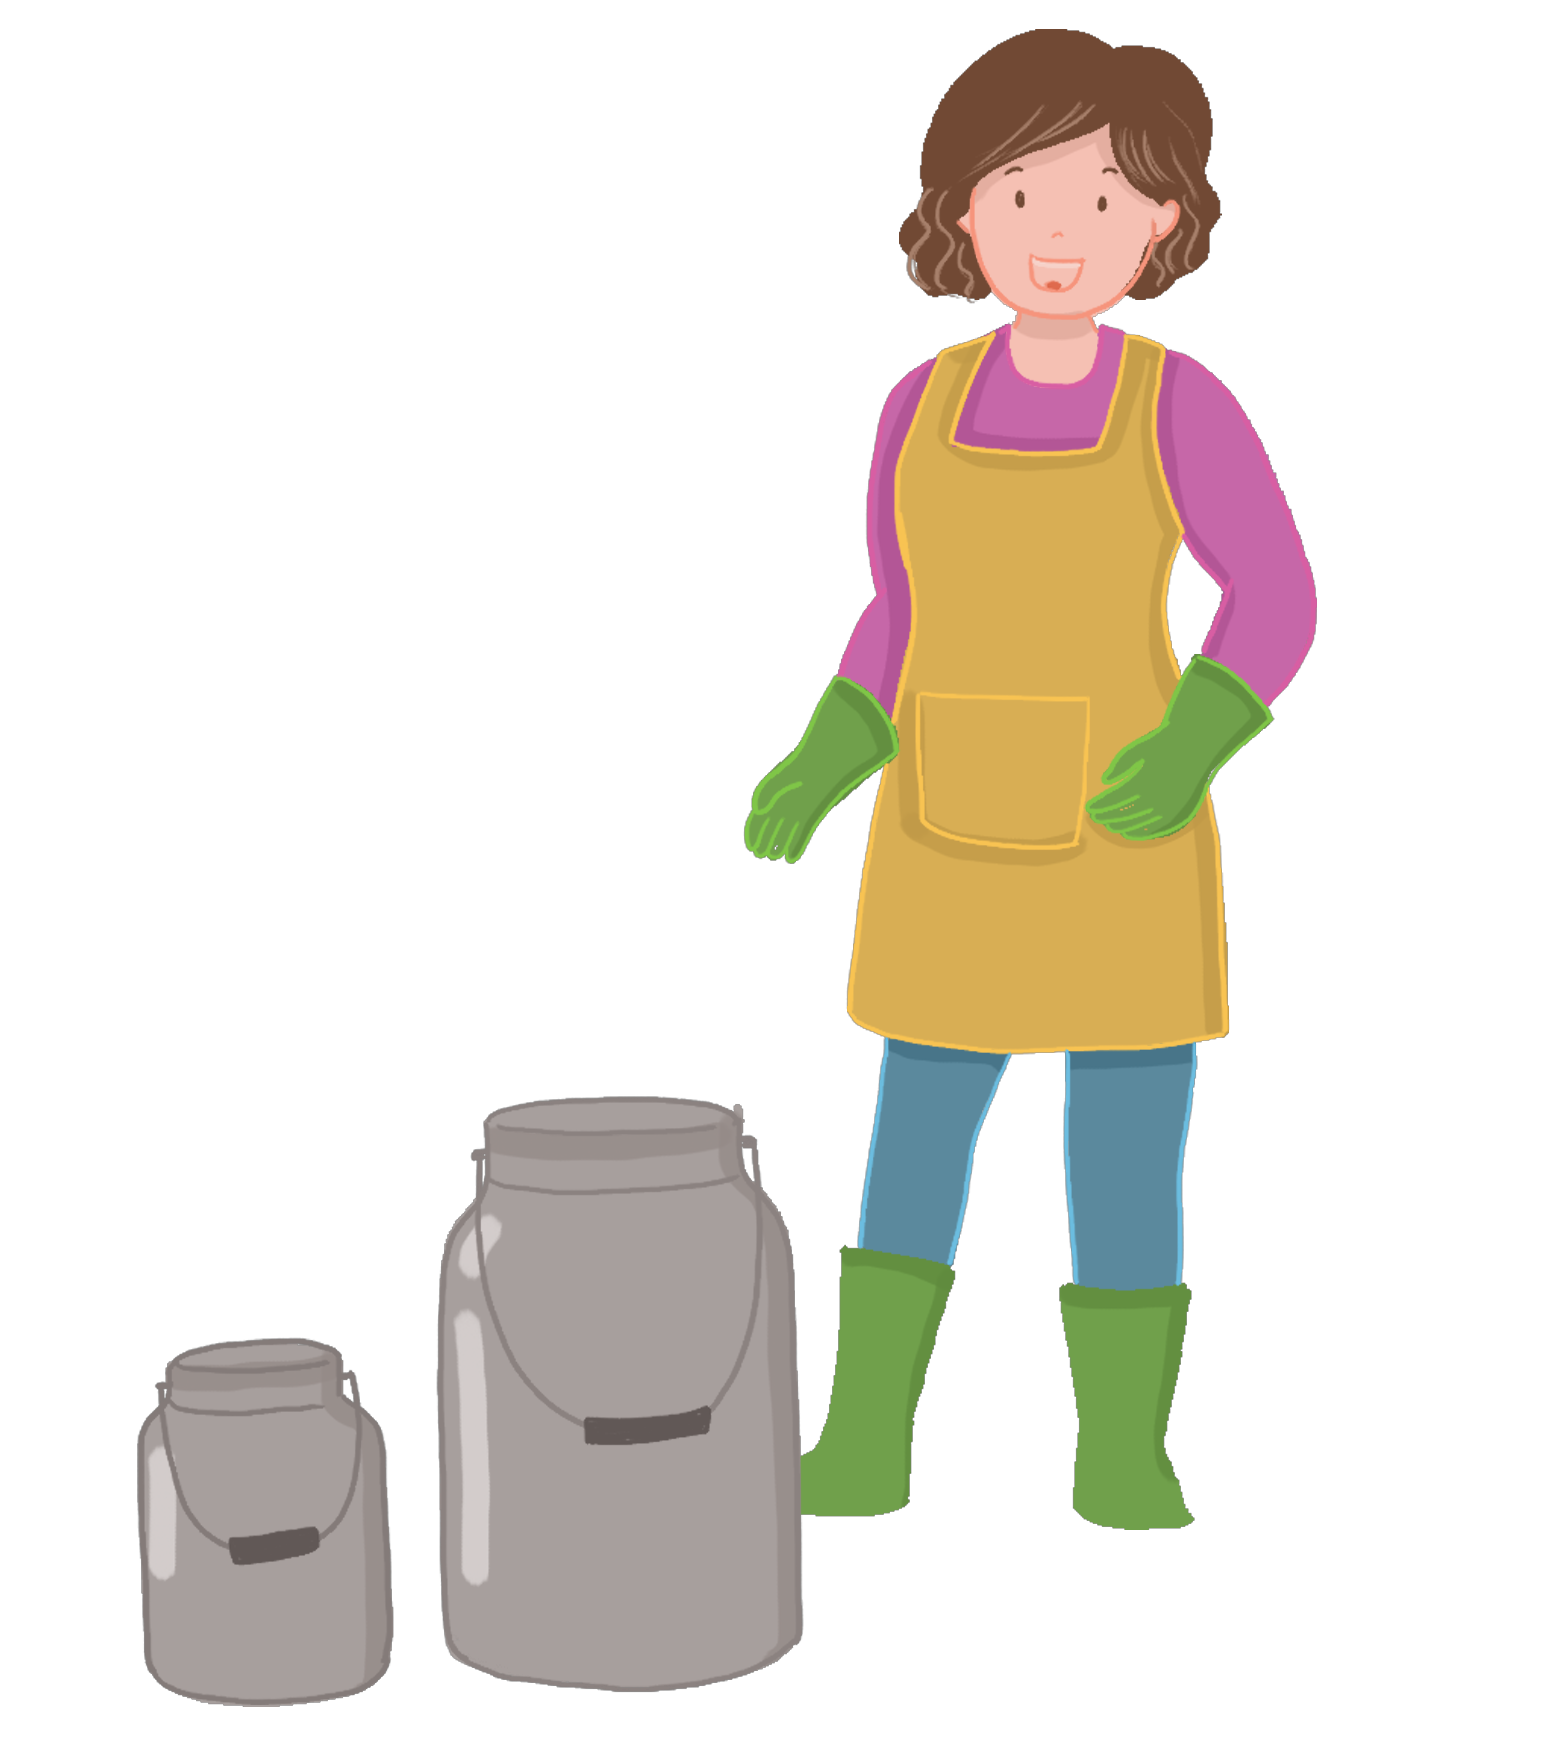
\includegraphics[width=0.75\linewidth]{Pi3_bai2}
		\vspace*{-5pt}
	\end{figure}
	$\pmb{3.}$ Một tấn hoa quả được chở tới siêu thị: táo được đóng theo các thùng gỗ  $48$ kg/thùng, lê được đóng trong các thùng gỗ $20$ kg/thùng, mận đựng trong hộp giấy theo $14$ kg/hộp còn nho đựng trong các hộp giấy theo $10$ kg/hộp. Biết rằng số kg táo được chở tới nhiều gấp đôi số kg lê, còn số kg mận và nho là bằng nhau, hỏi số lượng mỗi loại hoa quả đã được vận chuyển tới cửa hàng là bao nhiêu?
	\begin{figure}[H]
		\centering
		\vspace*{-5pt}
		\captionsetup{labelformat= empty, justification=centering}
		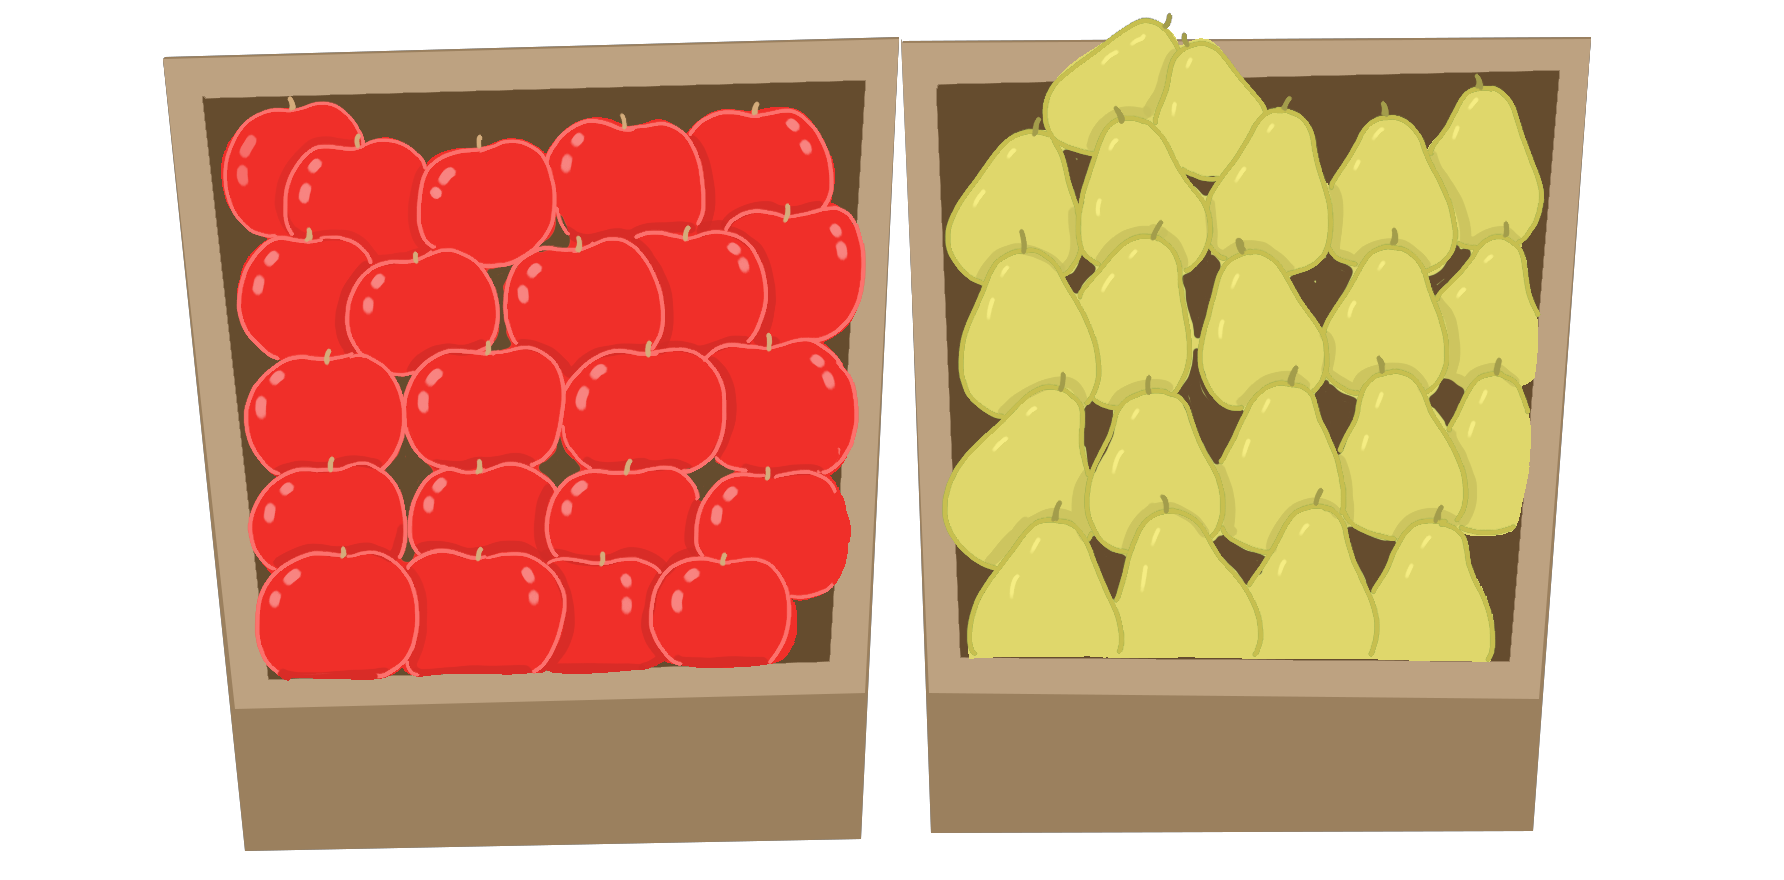
\includegraphics[width=1\linewidth]{Pi3_bai3}
		\vspace*{-10pt}
	\end{figure}
	$\pmb{4.}$ Bạn An khởi hành đi bộ từ làng $A$ tới làng $B$ lúc $8$h sáng. Đồng thời vào lúc đó, bạn Bình cũng đi bộ từ làng $B$ tới làng $A$. Hai bạn đều đi với vận tốc không đổi, nhưng có thể không bằng nhau. Khi gặp nhau ở giữa đường, bạn An còn phải đi thêm $32$ phút nữa, còn Bình phải đi thêm $18$ phút nữa thì mới tới nơi. Hỏi hai bạn đã gặp nhau sau bao lâu tính từ lúc khởi hành?
	\begin{figure}[H]
		\centering
		\vspace*{-5pt}
		\captionsetup{labelformat= empty, justification=centering}
		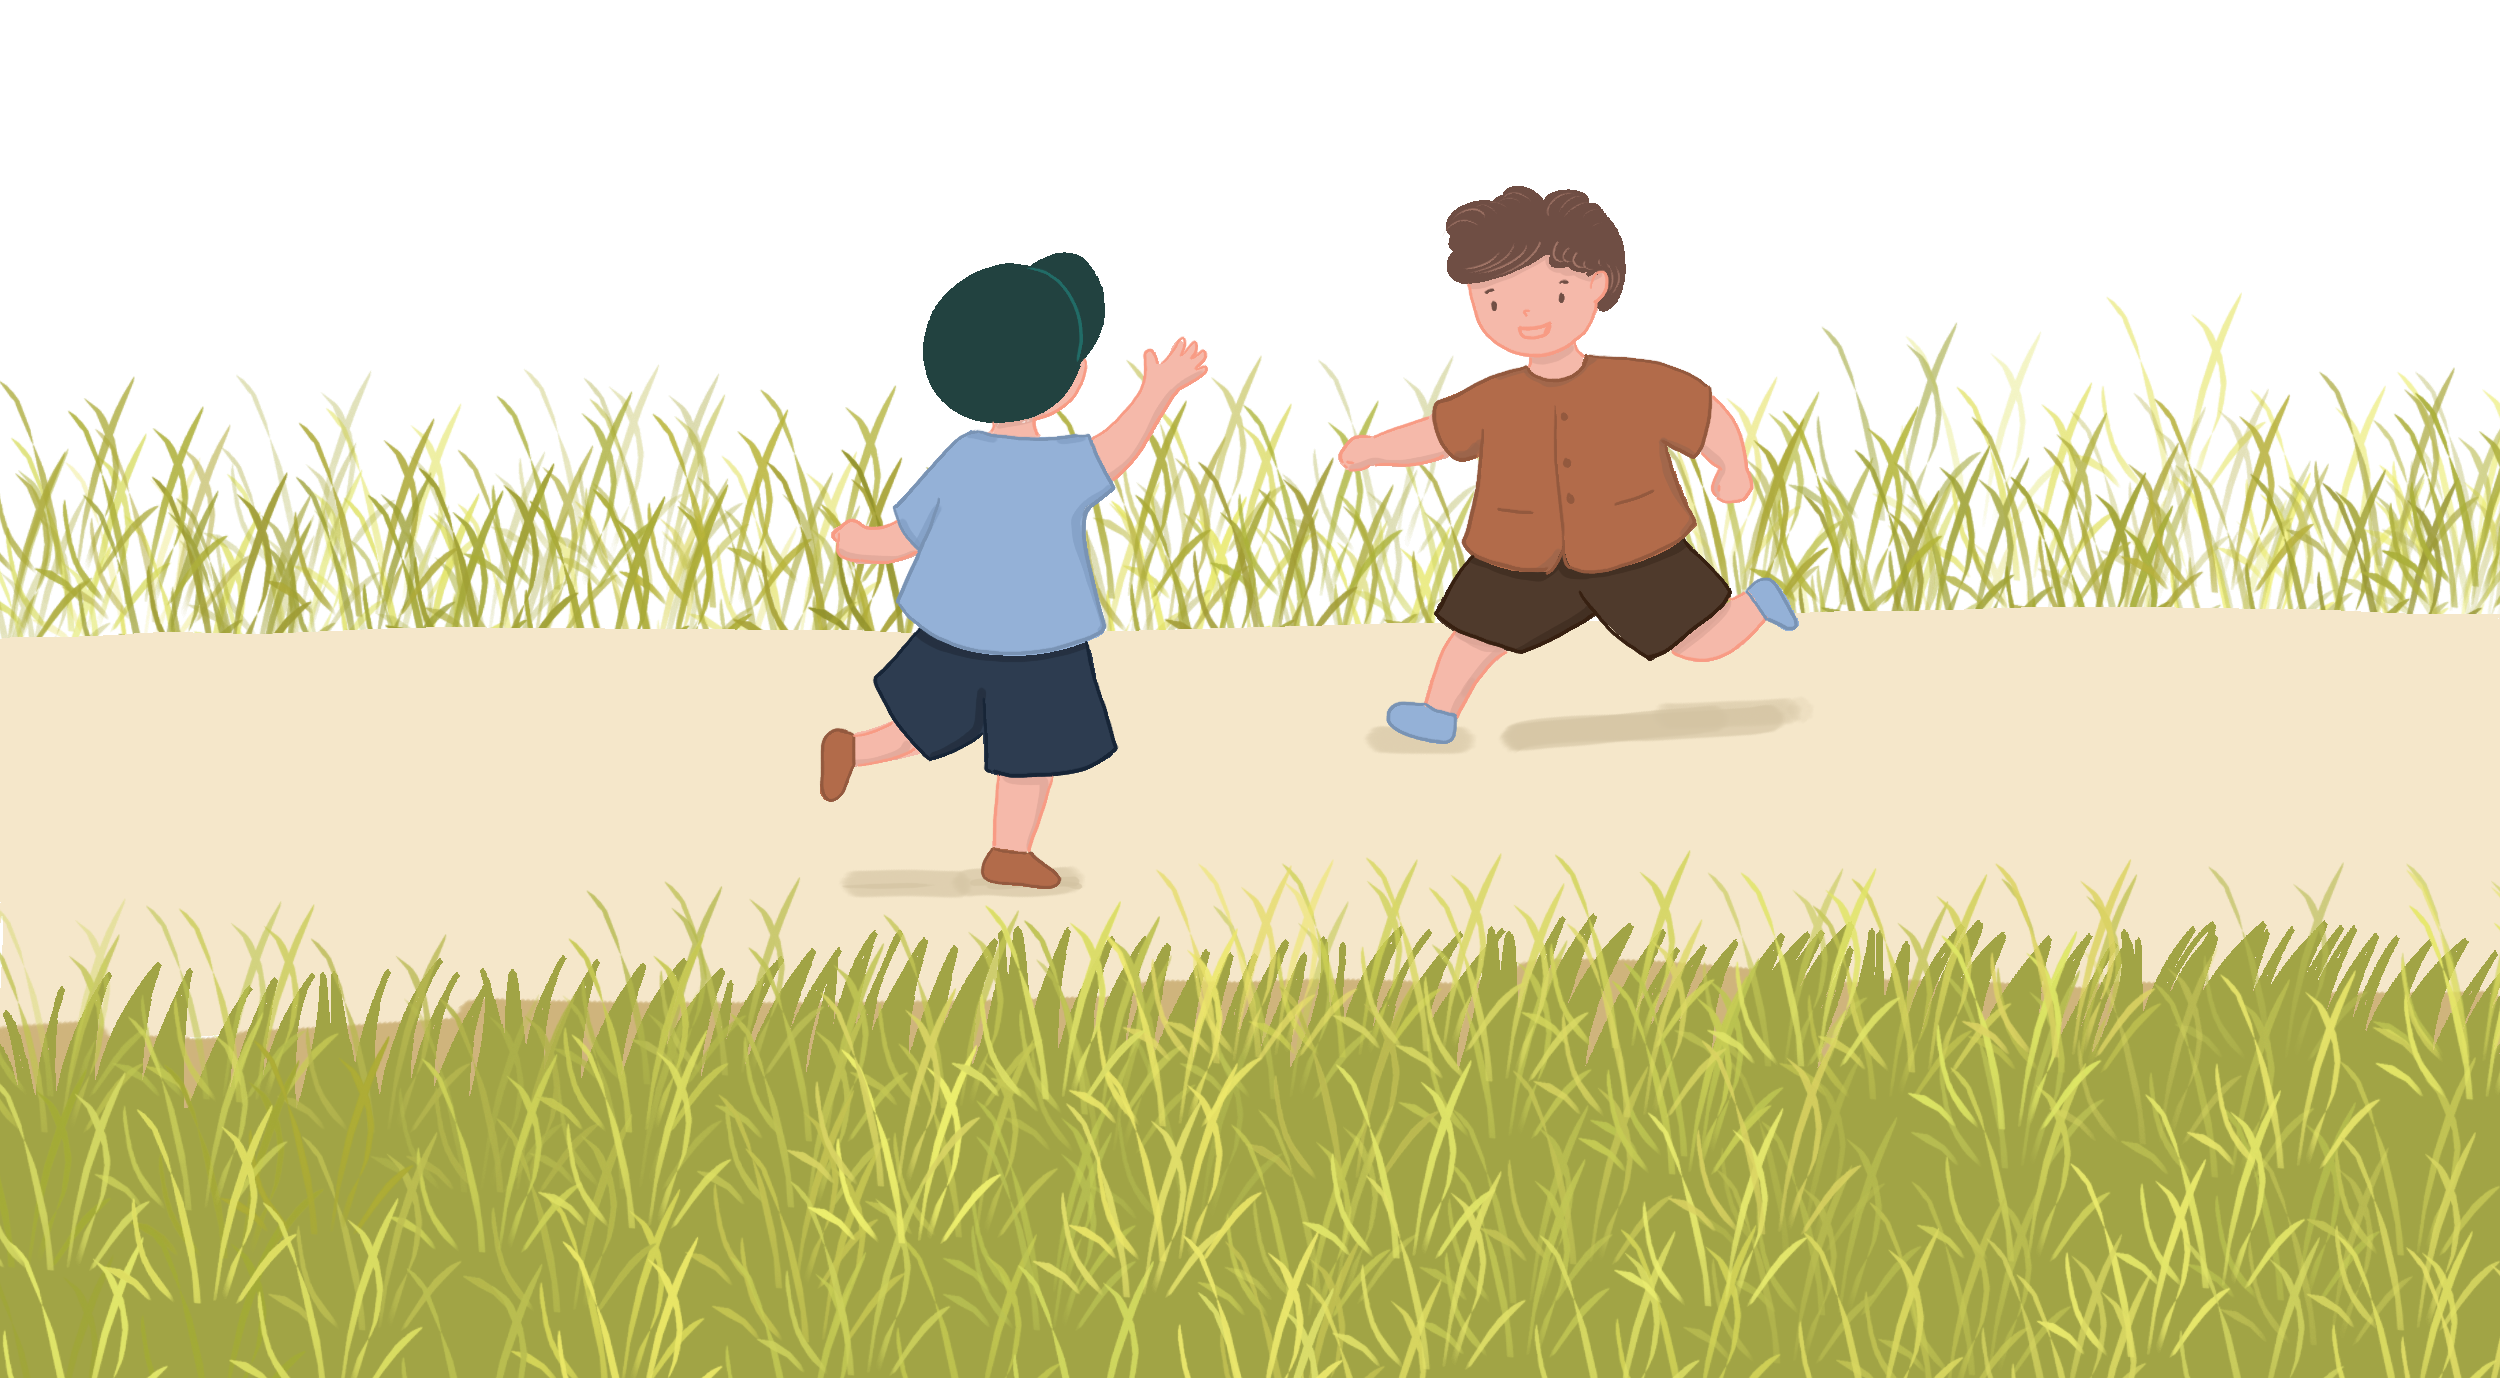
\includegraphics[width=1\linewidth]{Pi3_bai4}
		\vspace*{-10pt}
	\end{figure}
	$\pmb{5.}$ Trong một cuộc thi thể thao do nhà vua Pháp tổ chức, $3$ chàng ngự lâm pháo thủ là Athos, Porthos và Aramis cùng D'Artagnan chia nhau bốn vị trí đầu tiên: $1$, $2$, $3$, $4$ (ứng với giải thưởng: nhất, nhì, ba, bốn). Tổng ba số chỉ vị trí mà Athos, Porthos và D'Artagnan giữ là bằng $6$. Tổng hai số chỉ vị trí mà Porthos và Aramis giữ cũng bằng $6$. Hỏi mỗi chàng ngự lâm đã chiếm các giải nào, biết Porthos chiếm được giải cao hơn Arthos?
	\begin{figure}[H]
		\centering
		\vspace*{-5pt}
		\captionsetup{labelformat= empty, justification=centering}
		\includegraphics[width=1\linewidth]{Pi3_bai5}
		\vspace*{-15pt}
	\end{figure}
	$\pmb{6.}$ Tại một khách sạn nọ, nhân viên trực quản lý điều hành phải làm việc từ $8$h sáng tới $8$h tối (phương án $A$), hoặc từ $8$h tối tới $8$h sáng (phương án $B$), hoặc làm trọn cả ngày $24$h bắt đầu từ $8$h (sáng hoặc tối) (phương án $C$). Nếu làm theo phương án $A$, nhân viên trực quản lý sẽ được nghỉ không ít hơn $1$ ngày ($24$h). Nếu làm theo phương án $B$, nhân viên trực quản lý sẽ được nghỉ không ít hơn $1$ ngày rưỡi ($36$h). Còn nếu làm theo phương án $C$, nhân viên trực quản lý sẽ được nghỉ không ít hơn hai ngày rưỡi ($60$h).
	\vskip 0.1cm
	Hỏi khách sạn phải cần có ít nhất bao nhiêu nhân viên trực quản lý để đảm bảo lịch làm việc, nghỉ ngơi ở trên được tuân thủ?
\end{multicols}
\vspace*{-10pt}
{\color{toancuabi}\rule{1\linewidth}{0.1pt}}
\begingroup
\AddToShipoutPicture*{\put(110,405){\includegraphics[scale=1]{../tieude2.pdf}}} 
\centering
\endgroup
\vspace*{75pt}

\begin{multicols}{2}
	$\pmb{1.}$ Hai anh bạn rủ nhau đi câu cá. Khi được hỏi ``Trong mỗi giỏ của các anh có bao nhiêu con cá đấy?" thì anh thứ nhất trả lời ``Trong giỏ của tôi có số cá bằng nửa số cá ở giỏ của anh kia và thêm $10$ con nữa". Anh thứ hai lại nói ``Còn trong giỏ của tôi có số cá bằng số cá trong giỏ của anh kia và thêm $20$ con nữa". Vậy cả hai anh bạn có tất cả bao nhiêu con cá nhỉ? 
	\begin{figure}[H]
		\centering
		\vspace*{-10pt}
		\captionsetup{labelformat= empty, justification=centering}
		\includegraphics[width=1\linewidth]{Pi10_ToanBi_Bai1}
		\vspace*{-15pt}
	\end{figure}
	\textit{Lời giải.} Một nửa số cá của anh thứ hai sẽ là nửa số cá của anh thứ nhất cộng thêm $10$ con. Vậy nửa số cá của anh thứ hai cộng thêm $10$ con sẽ bằng nửa số cá của anh thứ nhất cộng thêm $20$ con. Theo đề bài, số cá này bằng cả số cá của anh thứ nhất.
	\vskip 0.1cm
	Vậy một nửa số cá của anh thứ nhất là: $20$ (con)
	\vskip 0.1cm
	Suy ra anh thứ nhất có số cá là
	\begin{align*}
		2 \times 20 = 40 \text{  (con)}
	\end{align*}
	và anh thứ hai có số cá là 
	\begin{align*}
		40+20 = 60 \text{  (con).}
	\end{align*} 
	Tổng số cá của cả hai anh là 
	\begin{align*}
		40+60 = 100 \text{  (con).}
	\end{align*}
	Đây là bài tập đơn giản, tuy nhiên các em thử tập làm bằng nhiều cách khác nhau thông qua suy luận thông thường mà không cần dùng tới cách lập phương trình nhé.
	\vskip 0.1cm
	$\pmb{2.}$ Lọ lem có $100$ rổ đựng hạt dẻ, lúc đầu số hạt dẻ trong mỗi rổ là như nhau. Lọ Lem lấy đi trong rổ thứ nhất một số hạt dẻ, lấy từ rổ  thứ hai một số hạt gấp đôi như thế, lấy từ rổ thứ ba một số hạt gấp ba như thế, và cứ như vậy. Cuối cùng thì trong rổ thứ $100$ chỉ còn đúng một hạt dẻ, và còn lại ở tất cả trong $100$ rổ tổng cộng là $14950$ hạt dẻ. Hỏi ban đầu trong mỗi rổ có bao nhiêu hạt dẻ?
	\begin{figure}[H]
		\centering
		\vspace*{-10pt}
		\captionsetup{labelformat= empty, justification=centering}
		\includegraphics[width=1\linewidth]{Pi10_ToanBi_Bai2}
		\vspace*{-15pt}
	\end{figure}
	\textit{Lời giải.} 	Gọi số hạt dẻ mà Lọ Lem lấy ở rổ thứ nhất là $a$, khi đó tổng cộng số hạt dẻ mà Lọ lem đã lấy đi ở $100$ rổ là
	\begin{align*}
		a+ 2a+\cdots+100a=5050a.
	\end{align*} 
	Do rổ cuối cùng còn lại $1$ hạt dẻ nên ban đầu số hạt dẻ ở rổ cuối cùng (cũng là số hạt dẻ ở các rổ khác) là: $100a+1$ (hạt).
	\vskip 0.1cm
	Vậy, ban đầu tổng số hạt dẻ là
	\begin{align*}
		100\times(100a+1) = 10000a+100 \text{  (hạt).}
	\end{align*} 
	Ta có hệ thức là: $10000a+100-5050 a =14950$. Từ đó suy ra $a=3$. Vì vậy ban đầu mỗi rổ có  $100\times 3+1 = 301$ hạt dẻ.
	\vskip 0.1cm
	$\pmb{3.}$ Hai bạn học sinh là Nam và Vũ gặp nhau tại nhà của Vũ. Nam nói ``Nếu lấy số nhà của tớ là một số có hai chữ số trừ đi số có hai chữ số tạo thành khi viết theo thứ tự ngược lại, thì sẽ ra số nhà của cậu. Vậy tớ sống ở số nhà nào?"
	\vskip 0.1cm
	Vũ trả lời ``Ôi, bài toán này dễ quá" -- và giải ra luôn đáp số.
	\vskip 0.1cm
	Vậy các bạn đó sống ở những số nhà nào nhỉ?
	\vskip 0.1cm
	\textit{Lời giải.} 	Nếu thực hiện phép trừ của Nam, ta sẽ nhận được số có dạng $9\times k$, ở đó $k$ là hiệu của chữ số hàng chục và chữ số hàng đơn vị. Vì số viết theo thứ tự ngược lại cũng là số có hai chữ số, nên $k\le8$. 
	\vskip 0.1cm
	Nếu $k<8$ thì có thể thấy có nhiều số có hai chữ số (là số nhà) mà sau khi làm phép tính trừ đã cho sẽ cho kết quả như nhau. Khi đó Vũ không thể giải được ngay câu đố của Nam. Do đó $k=8$. Các em có thể tìm thấy số nhà của Nam là $91$, và số nhà của Vũ là $72$.
	\begin{figure}[H]
		\centering
		\vspace*{-5pt}
		\captionsetup{labelformat= empty, justification=centering}
		\includegraphics[width=1\linewidth]{Pi10_ToanBi_Bai3}
		\vspace*{-15pt}
	\end{figure}
	$\pmb{4.}$ Lớp của Hùng có $35$ học sinh. Trong số đó có $20$ em tham gia câu lạc bộ Toán, $11$ em tham gia câu lạc bộ Khéo tay, $10$ em không tham gia vào hai nhóm này. Hỏi có tất cả bao nhiêu em vừa tham gia CLB Toán lại vẫn không quên tham gia cả CLB Khéo tay nhỉ?
	\begin{figure}[H]
		\centering
		\vspace*{-5pt}
		\captionsetup{labelformat= empty, justification=centering}
		\includegraphics[width=1\linewidth]{Pi10_ToanBi_Bai4}
		\vspace*{-15pt}
	\end{figure}
	\textit{Lời giải.} 	Chúng ta chia toàn bộ số học sinh trong lớp thành bốn danh sách, mà không có em nào ở trong hai danh sách khác nhau, như sau. Danh sách ``toán thuần tuý" gồm các bạn chỉ tham gia CLB Toán, danh sách ``khéo tay thuần tuý" gồm các bạn chỉ tham gia CLB Khéo tay, danh sách ``giỏi toán lại khéo tay" gồm các bạn tham gia cả $2$ CLB  và cuối cùng là danh sách ``rảnh rỗi" là các bạn không tham gia vào hai CLB này. Theo đề bài, danh sách ``rảnh rỗi" có $10$ bạn, vì thế có $25$ bạn không ``rảnh rỗi". Trong số $25$ bạn này có $20$ bạn tham gia nhóm Toán, vì thế số ``khéo tay thuần tuý" là $5$ bạn. Vậy số bạn vừa tham gia nhóm Toán lại ``khéo tay" nữa là 
	\begin{align*}
		11-5 = 6 \text{ (bạn).}
	\end{align*}
	$\pmb{5.}$ Tùng đến trường mới có nhiều chuyện rất vui nên về khoe với bạn bè.
	\begin{figure}[H]
		\centering
		%		\vspace*{5pt}
		\captionsetup{labelformat= empty, justification=centering}
		\includegraphics[width=1\linewidth]{Pi10_ToanBi_Bai5}
		\vspace*{-15pt}
	\end{figure}
	-- Lớp tớ có $35$ học sinh. Và các cậu có tưởng tượng được không, mỗi người lại kết bạn với đúng $11$ học sinh cùng lớp.
	\vskip 0.1cm
	-- Không thể thế được! Bách, người bạn thân của Tùng vừa đạt giải trong một cuộc thi Olympic, ngay lập tức trả lời.
	\vskip 0.1cm
	Vì sao Bách lại nghĩ như vậy nhỉ?
	\vskip 0.1cm
	\textit{Lời giải.} 	Ta biểu diễn mỗi học sinh được thể hiện bởi một điểm. Nếu hai học sinh kết bạn với nhau ta sẽ nối hai điểm tương ứng bởi một đoạn thẳng. Như vậy có $35$ điểm, mỗi điểm được nối đúng với $11$ điểm khác. Khi đó tổng số các đầu của các đoạn thẳng nối quan hệ bạn bè là $35\times11$ là một số lẻ. Điều này là vô lý do mỗi đoạn thẳng thể hiện quan hệ bạn bè có đúng hai điểm đầu mút. 
	\vskip 0.1cm
	$\pmb{6.}$ Có $55$ em học sinh tham gia một cuộc thi Olympic. Tất cả các em đều nộp bài. Khi chấm bài, mỗi câu hỏi được chấm bởi một trong ba loại điểm: điểm ``$+$" nếu câu hỏi được trả lời hoàn toàn đúng; điểm ``$-$" nếu câu hỏi đã có trả lời nhưng chưa ra đúng đáp số; và điểm ``$0$" nếu câu hỏi chưa được trả lời. Sau khi chấm toàn bộ bài thi, ban tổ chức thấy không có hai bài thi nào có cả các số điểm ``$+$" và số điểm ``$-$" đồng thời trùng nhau. Vậy trong kỳ thi Olympic đó phải có ít nhất bao nhiêu câu hỏi?
	\vskip 0.1cm
	\textit{Lời giải.} 	Giả sử $a$ là số câu hỏi được ra.  Ta chia ra các trường hợp sau
	\vskip 0.1cm
	$1.$ Bài thi có tất cả các câu hỏi đều được trả lời: Khi đó số các bài thi sẽ không vượt quá $a+1$ bài: từ bài có $a$ dâú ``$+$" và $0$ dấu ``$-$" cho đến bài có $0$ dấu ``$+$" và $a$ dấu ``$-$".  
	\vskip 0.1cm
	Bài thi trong đó chỉ có đúng một bài chưa có trả lời (có một điểm ``$0$"): Số các bài thi  nhiều nhất là $a$ bài (từ $a-1$ điểm ``$+$" và $0$ điểm ``$-$" cho đến bài có $0$ điểm ``$+$" và $a-1$ điểm ``$-$"). $\ldots$
	\vskip 0.1cm
	Và cứ xét như vậy, ta thấy tổng số các bài thi nhiều nhất là 
	\begin{align*}
		(a\!+\!1)\!+\!a\!+\!(a\!-\!1)\!+\!\cdots\!+\!1=\dfrac{(a\!+\!1)(a\!+\!2)}{2}.
	\end{align*}
	Từ đó ta có $55\le\dfrac{(a+1)(a+2)}{2}$. Với $a=9$ ta có $\dfrac{10\cdot11}{2}=55$. Vậy là $a \ge 9$. 
	\vskip 0.1cm
	Vì vậy số câu hỏi ít nhất được ra là $9$ câu.
\end{multicols}
\newpage
\begingroup
\thispagestyle{toancuabinone}
\blfootnote{$^1$\color{toancuabi}Ottawa, Canada.}
\AddToShipoutPicture*{\put(60,733){\includegraphics[width=17.2cm]{../mathc.pdf}}}
%\AddToShipoutPicture*{\put(-2,733){\includegraphics[width=17.2cm]{../mathl.pdf}}} 
\AddToShipoutPicture*{\put(125,675){\includegraphics[scale=1]{../tieude5.pdf}}} 
\centering
\endgroup
\graphicspath{{../toancuabi/pic/}}
\vspace*{33pt}

\begin{multicols}{2}
		In this article, we show a few example problems that can be solved when using the counting in two ways method.
		\vskip 0.2cm
		\PIbox{\textbf{\color{toancuabi}Example} (Sum of areas)\textbf{\color{toancuabi}.}
			$ABCD$ is a parallelogram. $E$ and $F$ are points on $AB$ and $BC,$ respectively.
			Lines $AF, CE, DE,$ and $DF$ dissect the parallelogram into $8$ regions,
			where some of them have known areas, as shown below in the diagram.
			\vskip 0.1cm
			Find the sum of the areas $a+b+c.$}
		\begin{figure}[H]
			\centering
			\vspace*{-5pt}
			\captionsetup{labelformat= empty, justification=centering}
			\includegraphics[width=1\linewidth]{hc-2022-2-2-6.pdf}
			\vspace*{-10pt}
		\end{figure}
		\textit{Solution.}
		From the properties of the parallelogram $ABCD,$ the following triangle pairs, with the same base and height, have the same area
		\begin{align*}
			\left.
			\begin{aligned}
				[AFB] = [DFB]\\
				[CEB] = [DEB]
			\end{aligned}
			\right\}
			\Rightarrow& [AFB] + [CEB] \\
			&= [DFB] + [DEB] \\
			&= [DEBF]
		\end{align*}
		Therefore
		\begin{align*}
			&(a + 47 + b) + (c + 32 + b)\\
			= \,&(323 + 47 + b + 32)\\
			\Rightarrow\, &a + b + c = 323.
		\end{align*}
		\vspace*{0.1pt}
		
		\vspace*{-6pt}
		\PIbox{\textbf{\color{toancuabi}Example} (How many knights are needed to protect King Anthony?)\textbf{\color{toancuabi}.}
			King Anthony went for hunting trip with his knights.
			At night, they stayed in one of the king's hunting lodges in the forest.
			In this house, there are nine rooms. The king slept in the central room.
			The knights stayed in the eight surrounding rooms such that
			in each direction north, south, east, west the total number of knights 
			in the \textit{three rooms} facing that direction should always be \textit{nine}.
			\textit{For example, the diagram below shows a possible case with each room has 3 knights.
			The letter $K$ indicates the King staying in the central room.}
			\begin{table}[H]
				\vspace*{-5pt}
				\centering
				\captionsetup{labelformat= empty, justification=centering}
				\renewcommand{\arraystretch}{1.2}
				\begin{tabular}{|c|c|c|}
					\hline
					$3$ & $3$    & $3$ \\ \hline
					$3$ & K & $3$ \\ \hline
					$3$ & $3$    & $3$ \\ \hline
				\end{tabular}
				\vspace*{-5pt}
			\end{table}
			What would be the smallest number of knights were with the king?
			What would be the largest?}
		\vskip 0.1cm
		\textit{Solution.}
			Let $a_1,a_2,a_3,a_4,b_1,b_2,b_3,$ and $b_4$ be the numbers of knights in each room as shown in the diagram.
			Let $S=a_1+a_2+a_3+a_4+b_1+b_2+b_3+b_4,$ then
			\begin{align*}
				&36 = (a_1\!+\!b_1\!+\!a_2)\!+\!(a_2\!+\!b_2\!+\!a_3)\\
				&\quad\quad\!+\!(a_3\!+\!b_4\!+\!a_4)\!+\!(a_4\!+\!b_4\!+\!a_1)\\
				\Rightarrow&
				\begin{cases}
					S = 36 - (a_1+a_2+a_3+a_4)\\
					S = \frac{1}{2}\left(36 + (b_1+b_2+b_3+b_4)\right)
				\end{cases}
			\end{align*}
			\begin{table}[H]
				\vspace*{-5pt}
				\centering
				\captionsetup{labelformat= empty, justification=centering}
				\begin{tabular}{|c|c|c|}
					\hline
					$a_1$ & $b_1$ & $a_2$ \\ \hline
					$b_4$ & K & $b_2$ \\ \hline
					$a_4$ & $b_3$ & $a_3$ \\ \hline
				\end{tabular}
				\caption{\small\textit{\color{toancuabi}With variables}}
				\vspace*{-10pt}
			\end{table}
			Thus, the least value of $S$ is $18$, if $b_1=b_2=b_3=b_4=0,$ and $a_1=a_3=5,a_2=a_4=4.$
			The most value of $S$ is $36$, if $a_1=a_2=a_3=a_4=0,$ and $b_1=b_2=b_3=b_4=9.$
		\vskip 0.2cm
		\PIbox{\textbf{\color{toancuabi}Example} (What are the family names of the sisters?)\textbf{\color{toancuabi}.}
			Four pairs of brother--sister share $32$ cookies.
			For the sisters, Lan got one, Mai got two, Na got three, and Quynh got four cookies.
			Danny Tran took as many as his sister, Elvin Nguyen twice as many as his sister,
			Franklin Pham three times as his sister, and Williams Quach four times as many as his sister.
			\vskip 0.1cm
			What are the family names of the girls?}
		\vskip 0.2cm
		\textit{Solution.}
			Let $x, 2y, 3z,$ and $4w$ be the numbers of cookies that 
			Danny Tran, Elvin Nguyen, Franklin Pham, and Williams Quach took.
			Their sisters took $x, y, z,$ and $w$ cookies respectively. Therefore,
			\begin{align*}
				&x + 2y + 3z + 4w + x + y + z + w = 32\\
				\Rightarrow &2x + 3y + 4z + 5w = 32.
			\end{align*}
			Note that $x, y, z, w$ are a permutation of $1,2,3,4,$ so $x + y + z + w = 10.$
			Thus 
			\begin{align*}
				&-x + z + 2w \!=\! 32-3(x + y + z + w) \!=\! 2 \\
				\Rightarrow \,&x > z, x \text{\ and\ } z \text{\ have the same parity}\\
				\Rightarrow\,&-x+z=-2 \Rightarrow  w=2 \\
				\Rightarrow \,&x=3, z=1, y=4. 
			\end{align*}
			Now, Lan got one, Mai got two, Na got three, and Quynh got four cookies.
			\vskip 0.1cm
			$x=3,$ so the girl who took three cookies, Na, is the sister of Danny Tran, so she is Na Tran.
			\vskip 0.1cm
			$y=4,$ so the girl who took four cookies, Quynh, is the sister of Elvin Nguyen, so she is Quynh Nguyen.
			\vskip 0.1cm
			$z=1,$ so the girl who took one cookie, Lan, is the sister of Franklin Pham, so she is Lan Pham.
			\vskip 0.1cm
			$w=2,$ so the girl who took two cookies, Mai, is the sister of Williams Quach, so she is Mai Quach.
			\vskip 0.1cm
			Hence, the girls's names are Na Tran, Quynh Nguyen, Lan Pham, and Mai Quach.
\end{multicols}
	
%	\newpage
%	
%	\setcounter{figure}{0}
%	\thispagestyle{thachthuctoanhocnone}
\pagestyle{thachthuctoanhoc}
\everymath{\color{thachthuctoanhoc}}
\graphicspath{{../thachthuctoanhoc/pic/}}
\begingroup
\AddToShipoutPicture*{\put(0,616){\includegraphics[width=19.3cm]{../thachthuctoanhoc/bannerthachthuc}}}
\centering
\vspace*{4cm}
\endgroup
\vspace*{-8pt}
\begin{tBox}
	\begin{itemize}[leftmargin = 13pt, itemsep = 1.0pt] 
		\item Mỗi bài toán đề xuất (kèm theo lời giải) cần được nêu rõ là bài sáng tác hay bài sưu tầm.
%				\item Mỗi bài toán đề xuất (kèm theo lời giải) cần được nêu rõ là bài sáng tác hay bài sưu tầm (nếu là bài sưu tầm, cần ghi rõ nguồn).
		\item Bài giải cho mỗi bài toán cần được trình bày trong một file riêng hoặc
		một tờ giấy riêng.
		\item  Người đề xuất bài toán hoặc gửi bài giải cho các bài toán trong mục ``Thách thức kỳ này" cần ghi rõ họ, đệm, tên và nơi làm việc/học tập, số điện thoại liên hệ. Nếu là học sinh (hoặc sinh viên) cần ghi rõ là học sinh lớp mấy (hoặc sinh viên năm thứ mấy).
		\item Các bài toán trong mục Thách thức kỳ này hướng tới các độc giả là học sinh phổ thông; được phân chia thành các mức độ $B$, $A$, và được sắp xếp theo độ khó tăng dần, theo đánh giá chủ quan của Ban biên tập. Các bài toán mức độ $B$ không đòi hỏi các kiến thức vượt quá chương trình môn Toán cấp THCS; các bài toán mức độ $A$ không đòi hỏi các kiến thức vượt quá chương trình môn Toán cấp THPT.
		\item Cách thức gửi bài toán đề xuất hoặc lời giải: gửi file thu được bằng cách scan, ảnh chụp (rõ nét) của bản viết tay, hoặc được soạn thảo bằng các phần mềm Latex, Word tới \url{bbt@pi.edu.vn} hoặc gửi qua đường bưu điện tới Tòa soạn (xem địa chỉ tại bìa $2$).
		\item Hạn gửi lời giải cho các bài toán P$681$--P$690$: trước ngày $15/4/2023$.
	\end{itemize}
\end{tBox}
\begin{center}
	\vspace*{-5pt}
	\textbf{\color{thachthuctoanhoc}\color{thachthuctoanhoc}\color{thachthuctoanhoc}THÁCH THỨC KỲ NÀY}
	\vspace*{-5pt}
\end{center}
\begin{multicols}{2}
	\setlength{\abovedisplayskip}{4pt}
	\setlength{\belowdisplayskip}{4pt}
	{\color{thachthuctoanhoc}{\usefont{T5}{qag}{b}{n} P681.}}
	(Mức $B$) Xét năm số nguyên khác nhau $a,b,c,d,e$ sao cho tổng của ba số bất kỳ trong chúng lớn hơn tổng của hai số còn lại. Tìm giá trị nhỏ nhất của tổng 
	\begin{align*}
		S=abcd+abce+abde+acde+bcde.
	\end{align*}
	\begin{flushright}
		\textit{Nguyễn Đức Tấn, Tp. Hồ Chí Minh (st)}
	\end{flushright}
	{\color{thachthuctoanhoc}{\usefont{T5}{qag}{b}{n} P682.}}
	(Mức $B$) Bạn Tâm nghĩ trong đầu một số nguyên lớn hơn $2$ và nhỏ hơn $26$. Bạn An hỏi bạn Tâm ba câu hỏi sau, về số mà bạn Tâm nghĩ:  
	\vskip 0.05cm
	-- Số đó có phải là số chính phương không?
	\vskip 0.05cm
	-- Số đó có phải là số nguyên tố không?
	\vskip 0.05cm
	-- Số đó có chia hết cho $n$ không?, 
	\vskip 0.05cm
	trong đó, $n$ là một số tự nhiên chẵn có một chữ số, do An tự chọn. 
	\vskip 0.05cm
	Biết rằng, căn cứ câu trả lời của Tâm cho ba câu hỏi trên, An đã đoán ra được chính xác số Tâm nghĩ trong đầu. Hỏi, An đã chọn số $n$ nào, và số Tâm nghĩ là số nào?
	\begin{flushright}
		\textit{Đặng Hải Hà, Hưng Yên (st)}
	\end{flushright}
	{\color{thachthuctoanhoc}{\usefont{T5}{qag}{b}{n} P683.}}
	(Mức $B$) Giả sử $a,b$ là các số dương, sao cho $a+b+\dfrac1a+\dfrac1b$ và $a^3+b^3+\dfrac1{a^3}+\dfrac1{b^3}$ đều là các số hữu tỷ. Chứng minh rằng, $a^2+b^2+\dfrac1{a^2}+\dfrac1{b^2}$ cũng là một số hữu tỷ. 
	\begin{flushright}
		\textit{NguyễnTường Thanh, Nghệ An (st)}
	\end{flushright}
	{\color{thachthuctoanhoc}{\usefont{T5}{qag}{b}{n} P684.}}
	(Mức $B$) Cho tam giác $ABC$ cân tại $A$, có $I$ là tâm đường tròn nội tiếp. Các đường thẳng $BI$ và $AC$ cắt nhau tại $D$. Gọi $E$ là điểm đối xứng của $I$ qua $D$; $O$ là tâm đường tròn ngoại tiếp tam giác $BCE$. Chứng minh rằng $OD\perp AC$. 
	\begin{center}
		\definecolor{ffqqqq}{rgb}{1,0,0}
		\definecolor{qqqqff}{rgb}{0,0,1}
		\definecolor{qqqqffa}{rgb}{1,1,1}
		\definecolor{cqcqcq}{rgb}{0.7529411764705882,0.7529411764705882,0.7529411764705882}
		\begin{tikzpicture}[thachthuctoanhoc,scale=0.6]
			\draw [line width=0.8pt] (0,7.5)-- (-3,0);
			\draw [line width=0.8pt] (-3,0)-- (3,0);
			\draw [line width=0.8pt] (3,0)-- (0,7.5);
			\draw [line width=0.8pt,color=ffqqqq] (0,2.5079796375600565) circle (3.9102380825744962cm);
			\draw [line width=0.8pt] (0,2.5079796375600565)-- (1.7213863318758427,3.1965341703103936);
			\draw [line width=0.8pt] (-3,0)-- (0,2.031098884280702);
			\draw [line width=0.8pt] (0,2.031098884280702)-- (1.7213863318758427,3.1965341703103936);
			\draw [line width=0.8pt] (0.8102365731004548,2.688342578037783) -- (0.9111497587753881,2.5392904765533135);
			\draw [line width=0.8pt] (1.7213863318758427,3.1965341703103936)-- (3.442772663751685,4.361969456340084);
			\draw [line width=0.8pt] (2.5316229049762966,3.8537778640674745) -- (2.6325360906512296,3.704725762583005);
			\draw [fill=qqqqffa] (0,7.5) circle (1.6pt);
			\draw[color=qqqqff] (-0.02,8.07) node {$A$};
			\draw [fill=qqqqffa] (-3,0) circle (1.6pt);
			\draw[color=qqqqff] (-3.32,-0.19) node {$B$};
			\draw [fill=qqqqffa] (3,0) circle (1.6pt);
			\draw[color=qqqqff] (3.14,-0.23) node {$C$};
			\draw [fill=qqqqffa] (0,2.031098884280702) circle (1.6pt);
			\draw[color=qqqqff] (0,1.69) node {$I$};
			\draw [fill=qqqqffa] (1.7213863318758427,3.1965341703103936) circle (1.6pt);
			\draw[color=qqqqff] (2.02,3.21) node {$D$};
			\draw [fill=qqqqffa] (3.442772663751685,4.361969456340084) circle (1.6pt);
			\draw[color=qqqqff] (3.7,4.67) node {$E$};
			\draw [fill=qqqqffa] (0,2.5079796375600565) circle (1.6pt);
			\draw[color=qqqqff] (-0.28,2.91) node {$O$};
		\end{tikzpicture}
	\end{center}
	\begin{flushright}
		\textit{Nguyễn Trường Minh, Hải Dương (st)}
	\end{flushright}
	{\color{thachthuctoanhoc}{\usefont{T5}{qag}{b}{n} P685.}}
	(Mức $B$) Tìm tất cả các số tự nhiên $x,y,z$ thoả mãn $(y-z)^4+1=2^x yz$. 
	\begin{flushright}
		\textit{Hà Duy Hưng, Hà Nội}
	\end{flushright}
	{\color{thachthuctoanhoc}{\usefont{T5}{qag}{b}{n} P686.}}
	(Mức $B$) Cho $a,b,c$ là các số thực dương có tổng bằng $3$.  Chứng minh rằng 
	\begin{align*}
		2\left(\dfrac1a+\dfrac1b+\dfrac1c\right)\ge a^2+b^2+c^2+3.
	\end{align*}
	\begin{flushright}
		\textit{Nguyễn Đông Dương}
	\end{flushright}
	{\color{thachthuctoanhoc}{\usefont{T5}{qag}{b}{n} P687.}}
	(Mức $A$) Cho $a,b,c,d,e,f$ là $6$ số hạng liên tiếp trong dãy Fibonacci. Trong mặt phẳng toạ độ, lấy các điểm $A(a;b)$, $B(c;d)$, $C(e;f)$
	Tính diện tích của tam giác $ABC$.
	\vskip 0.05cm
	(Dãy Fibonacci $(F_n)$ được xác định như sau: $F_0=0$, $F_1=1$ và $F_{n+2}=F_{n+1}+F_n$ với mọi $n\ge0$).
	\begin{flushright}
		\textit{Phùng Hồ Hải, Hà Nội}
	\end{flushright}
	{\color{thachthuctoanhoc}{\usefont{T5}{qag}{b}{n} P688.}}
	(Mức $A$) Xét các số thực $x,y,z$, thoả mãn $(x-1)^2+(y+2)^2+(z-1)^2=300$. Tìm giá trị lớn nhất và nhỏ nhất của biểu thức 
	\begin{align*}
		P=[x^2]+[y^2]+[z^2].
	\end{align*}
	\begin{flushright}
		\textit{Vũ Hồng Phong, Bắc Ninh}
	\end{flushright}
	{\color{thachthuctoanhoc}{\usefont{T5}{qag}{b}{n} P689.}}
	(Mức $A$) Cho tam giác nhọn $ABC$ nội tiếp đường tròn $(O)$, có trực tâm $H$, và $M$ là trung điểm $BC$. Qua $H$, kẻ đường thẳng $d$ cắt các cạnh $AB,AC$ lần lượt tại $F,E$. Gọi $K$ là tâm đường tròn ngoại tiếp tam giác $AEF$ và $J$ là trung điểm $EF$. Các đường thẳng $AK,AJ$ theo thứ tự cắt $(O)$ tại các điểm thứ hai $L,G$. Chứng minh rằng $\angle{MLG}=90^\circ$. 
	\begin{center}
		\definecolor{qqwwtt}{rgb}{0,0.4,0.2}
		\definecolor{ffqqqq}{rgb}{1,0,0}
		\definecolor{zzttqq}{rgb}{0.6,0.2,0}
		\definecolor{qqqqff}{rgb}{0,0,1}
		\definecolor{qqqqffa}{rgb}{1,1,1}
		\begin{tikzpicture}[thachthuctoanhoc,scale=0.6]
			\draw [line width=0.8pt,color=zzttqq] (-2.82,5.44)-- (-4.76,0);
			\draw [line width=0.8pt,color=zzttqq] (-4.76,0)-- (2.28,0);
			\draw [line width=0.8pt,color=zzttqq] (-2.82,5.44)-- (2.28,0);
			\draw [line width=0.8pt,color=ffqqqq] (-1.24,1.8106250000000004) circle (3.9583788210105664cm);
			\draw [line width=0.8pt] (-4.0820544984927425,1.9010430557729303)-- (0.795966931431351,1.5829686064732256);
			\draw [line width=0.8pt,color=qqwwtt] (-1.5612378815756844,2.996589290150962) circle (2.7485883591009133cm);
			\draw [line width=0.8pt] (-1.24,0)-- (-0.43160635518688706,-2.0643282391566697);
			\draw [line width=0.8pt] (0.797928735195991,-1.5828406858273176)-- (-0.43160635518688706,-2.0643282391566697);
			\draw [line width=0.8pt] (-2.82,5.44)-- (-0.43160635518688706,-2.0643282391566697);
			\draw [line width=0.8pt] (0.797928735195991,-1.5828406858273176)-- (-2.82,5.44);
			\draw [fill=qqqqffa] (-2.82,5.44) circle (1.6pt);
			\draw[color=qqqqff] (-2.84,5.89) node {$A$};
			\draw [fill=qqqqffa] (-4.76,0) circle (1.6pt);
			\draw[color=qqqqff] (-5,-0.31) node {$B$};
			\draw [fill=qqqqffa] (2.28,0) circle (1.6pt);
			\draw[color=qqqqff] (2.42,-0.25) node {$C$};
			\draw [fill=qqqqffa] (-1.24,0) circle (1.6pt);
			\draw[color=qqqqff] (-1.56,-0.27) node {$M$};
			\draw [fill=qqqqffa] (-2.82,1.81875) circle (1.6pt);
			\draw[color=qqqqff] (-2.92,1.55) node {$H$};
			\draw [fill=qqqqffa] (0.795966931431351,1.5829686064732256) circle (1.6pt);
			\draw[color=qqqqff] (1.14,1.83) node {$E$};
			\draw [fill=qqqqffa] (-4.0820544984927425,1.9010430557729303) circle (1.6pt);
			\draw[color=qqqqff] (-4.38,2.07) node {$F$};
			\draw [fill=qqqqffa] (-1.5612378815756847,2.996589290150963) circle (1.6pt);
			\draw[color=qqqqff] (-1.38,3.41) node {$K$};
			\draw [fill=qqqqffa] (-1.6430437835306957,1.742005831123078) circle (1.6pt);
			\draw[color=qqqqff] (-1.84,1.45) node {$J$};
			\draw [fill=qqqqffa] (-0.43160635518688706,-2.0643282391566697) circle (1.6pt);
			\draw[color=qqqqff] (-0.38,-2.29) node {$L$};
			\draw [fill=qqqqffa] (0.797928735195991,-1.5828406858273176) circle (1.6pt);
			\draw[color=qqqqff] (0.96,-1.85) node {$G$};
		\end{tikzpicture}
	\end{center}
	\begin{flushright}
		\textit{Đỗ Đại Phong, Tp. Huế}
	\end{flushright}
	{\color{thachthuctoanhoc}{\usefont{T5}{qag}{b}{n} P690.}}
	(Mức $A$) Cho biết, $\{1;2;3;4;5;6;7;$ $8;9\}$ là tập hợp tất cả các hệ số của ba tam thức bậc hai $f(x),g(x),h(x)$. Hỏi, có thể xảy ra hay không, trường hợp ba tam thức đó có nghiệm hữu tỷ chung?
	\begin{flushright}
		\textit{Lê Phúc Lữ, Tp. Hồ Chí Minh}
	\end{flushright}
\end{multicols}
\newpage
\centerline{{\large{\textbf{\color{thachthuctoanhoc}GIẢI BÀI KỲ TRƯỚC}}}}
\vspace*{-5pt}
\begin{multicols}{2}
	\setlength{\abovedisplayskip}{4pt}
	\setlength{\belowdisplayskip}{4pt}
	{\color{thachthuctoanhoc}{\usefont{T5}{qag}{b}{n} P651.}}
	(Mức $B$)
	Có hai chiếc hộp, mỗi hộp đều chứa các viên bi khác màu. Số viên bi đỏ ở hộp thứ nhất bằng $\dfrac{4}{15}$ số viên bi trong hộp đó. Tổng số viên bi đỏ ở hai hộp bằng $\dfrac{11}{25}$ tổng số viên bi của hai hộp. Hỏi, trong hai hộp có ít nhất bao nhiêu viên bi đỏ? Biết rằng, hộp thứ hai chứa $200$ viên bi.
	\vskip 0.05cm
	\textbf{\color{thachthuctoanhoc}Lời giải} (\textit{của người chấm bài})\textbf{\color{thachthuctoanhoc}.}
	\vskip 0.05cm
	Gọi $a$ (viên) là số viên bi đỏ có trong hộp thứ nhất, và gọi $s$ (viên) là tổng số viên bi đỏ của cả hai hộp; ta có, $a, s \in \mathbb{N^*}$. Theo bài ra, ta cần tìm giá trị nhỏ nhất của $s$.
	\vskip 0.05cm
	Vì số viên bi đỏ ở hộp thứ nhất bằng $\dfrac{4}{15}$  số viên bi trong hộp đó, nên số viên bi có trong hộp thứ nhất bằng  $d\dfrac{15a}{4}$. Do đó, theo giả thiết về tổng số viên bi đỏ của cả hai hộp, ta có:
	\begin{align*}
		s = \dfrac{{11}}{{25}}\left( {\dfrac{{15a}}{4} + 200} \right) = \dfrac{{33a}}{{20}} + 88. \tag{$1$}
	\end{align*}
	Từ đó, do $s \in \mathbb{N^*}$ và $a > 0$, suy ra  $\dfrac{33a}{20} \in \mathbb{N^*}$. Vì thế, $33a$ chia hết cho $20$; mà $(33, 20) = 1$, nên $a$ chia hết cho $20$. Suy ra, $a \ge 20$ (do  $a \in \mathbb{N^*}$). Vì vậy, từ ($1$) ta có:
	\begin{align*}
		s \ge \dfrac{{33 \cdot 20}}{{20}} + 88 = 121. \tag{$2$}	
	\end{align*}
	Tiếp theo, xét hai hộp bi, mà hộp thứ nhất chứa $75$ viên, trong đó có $20$ viên bi đỏ, và hộp thứ hai chứa $200$ viên, trong đó có $101$ viên bi đỏ, ta có:
	\begin{align*}
		20 = \dfrac{4}{{15}} \cdot 75 \text{ và } 20 + 101 = \dfrac{{11}}{{25}}\left( {75 + 200} \right).
	\end{align*}
	Như vậy, hai hộp bi nói trên thỏa mãn tất cả các giả thiết của đề bài, và có tổng số viên bi đỏ ở cả hai hộp bằng $121$ viên. \hfill ($3$)
	\vskip 0.05cm
	Từ ($2$) và ($3$) suy ra, giá trị nhỏ nhất của $s$ là $121$. Nói một cách khác, trong hai hộp bi, thỏa mãn các giả thiết của đề bài, có ít nhất $121$ viên bi đỏ.
	\vskip 0.05cm
	\textbf{\color{thachthuctoanhoc}Bình luận và Nhận xét}
	\vskip 0.05cm	
	Rất tiếc, tất cả các lời giải Tạp chí đã nhận được từ bạn đọc đều không được coi là lời giải đúng, do người giải bài đã mắc một trong các lỗi sau:
	\vskip 0.05cm
	-- Khẳng định giá trị nhỏ nhất của $s$ (theo ký hiệu trong Lời giải trên) là $121$ \textit{ngay sau khi} chỉ mới chứng minh được $s \ge 121$;
	\vskip 0.05cm
	(\textit{Lỗi trên đây đã được nhắc nhở nhiều lần trong các số trước đây của Tạp chí!})
	\vskip 0.05cm
	-- Giải một bài toán khác, thay vì giải bài đã ra. Cụ thể, các bạn mắc lỗi này đã giải một trong hai bài toán dưới đây:
	\vskip 0.05cm
	+ Bài toán $1$: Với hai hộp bi thỏa mãn các giả thiết của bài đã ra, hãy tìm số viên bi đỏ nhỏ nhất có thể trong mỗi hộp.
	\vskip 0.05cm
	+ Bài toán $2$: Là bài toán nhận được từ bài đã ra, bằng cách thay giả thiết ``tổng số viên bi đỏ ở hai hộp bằng $\dfrac{11}{25}$ tổng số viên bi của hai hộp" bởi giả thiết ``số viên bi đỏ ở hộp thứ hai bằng $\dfrac{11}{25}$  tổng số viên bi của hai hộp".
	\begin{flushright}
		\textbf{\color{thachthuctoanhoc}Lê Huy}
	\end{flushright}
	{\color{thachthuctoanhoc}{\usefont{T5}{qag}{b}{n} P652.}}
	(Mức $B$) Chứng minh rằng, với hai số nguyên dương $a$, $b$, ta có thể tìm được số nguyên dương $c$, sao cho $a^2 + b^2 + c^2$  là một số chính phương, khi và chỉ khi $ab$ là một số chẵn.
	\vskip 0.05cm
	\textbf{\color{thachthuctoanhoc}Lời giải} (\textit{dựa theo các lời giải đúng, mà Tạp chí đã nhận được từ bạn đọc})\textbf{\color{thachthuctoanhoc}.}
	\vskip 0.05cm
	$\pmb{1.}$ \textit{Chứng minh ``khi".
	\vskip 0.05cm
	Giả sử $a$, $b$ là hai số nguyên dương có tích là một số chẵn. Ta cần chứng minh có thể tìm được số nguyên dương $c$, sao cho $a^2 + b^2 + c^2$  là một số chính phương.}
	\vskip 0.05cm
	Vì $ab$ là một số chẵn nên trong hai số nguyên dương $a$, $b$ có ít nhất một số chẵn. Do đó, xảy ra một trong hai trường hợp sau:
	\vskip 0.05cm
	$\diamond$ \textit{Trường hợp} $1$: Trong hai số $a$, $b$ có đúng một số chẵn.
	\vskip 0.05cm
	Khi đó, $a^2 + b^2$ là một số nguyên dương lẻ. Vì thế, tồn tại số nguyên dương $m$, sao cho
	\begin{align*}
		{a^2} + {b^2} = 2m + 1.
	\end{align*}
	Chọn $c = m$, ta có $c$ là số nguyên dương, và
	\begin{align*}
		{a^2} + {b^2} + {c^2} = 2m + 1 + {m^2} = {\left( {m + 1} \right)^2},
	\end{align*}
	là một số chính phương.
	\vskip 0.05cm
	$\diamond$ \textit{Trường hợp} $2$: Cả hai số $a$, $b$ đều là số chẵn.
	\vskip 0.05cm
	Khi đó, $a^2, b^2$  là các số chẵn chia hết cho $4$. Suy ra, $a^2 + b^2$ là một số nguyên dương chẵn chia hết cho $4$, và lớn hơn hoặc bằng $8$. Vì thế, tồn tại số nguyên dương $k \ge 2$, sao cho
	\begin{align*}
		{a^2} + {b^2} = 4k.
	\end{align*}
	Chọn $c = k - 1$, ta có $c$ là số nguyên dương, và
	\begin{align*}
		{a^2} + {b^2} + {c^2} = 4k + {\left( {k - 1} \right)^2} = {\left( {k + 1} \right)^2},
	\end{align*}
	là một số chính phương.
	\vskip 0.05cm
	Hiển nhiên, kết quả xét hai trường hợp trên cho ta điều cần chứng minh.
	\vskip 0.05cm
	$\pmb{2.}$ \textit{Chứng minh ``chỉ khi".}
	\vskip 0.05cm
	\textit{Giả sử $a$, $b$ là hai số nguyên dương, sao cho có số nguyên dương $c$, để $a^2 + b^2 + c^2$  là một số chính phương. Ta cần chứng minh ab là một số chẵn.}
	\vskip 0.05cm
	Giả sử $ab$ là một số lẻ. \hfill ($1$)
	\vskip 0.05cm
	Khi đó, cả hai số $a$, $b$ đều là số lẻ. Do đó, số dư trong các phép chia  $a^2$, $b^2$ cho $4$ đều là $1$. Suy ra, số dư trong phép chia $a^2 + b^2$  cho $4$ là $2$. Từ đây, do số dư trong phép chia $c^2$ cho $4$ là $0$ hoặc $1$, nên số dư trong phép chia $a^2 + b^2 + c^2$  cho $4$ sẽ là $2$ hoặc $3$. \hfill ($2$)
	\vskip 0.05cm
	Mặt khác, do $a^2 + b^2 + c^2$ là một số chính phương, nên số dư trong phép chia  $a^2 + b^2 + c^2$ cho $4$ chỉ có thể là $0$ hoặc $1$, mâu thuẫn với ($2$).
	\vskip 0.05cm
	Mâu thuẫn nhận được chứng tỏ giả sử ($1$) là sai. Vì thế, ta có điều cần chứng minh.
	\vskip 0.05cm
	\textbf{\color{thachthuctoanhoc}Bình luận và Nhận xét}
	\vskip 0.05cm
	Rất tiếc, có hơn nửa số lời giải, trong số tất cả các lời giải Tạp chí đã nhận được từ bạn đọc, là lời giải không đúng, do người giải bài đã mắc một trong các lỗi sau:
	\vskip 0.05cm
	-- Ở phần chứng minh ``khi", chưa chứng minh số $c$ được chọn là số dương;
	\vskip 0.05cm
	-- Chỉ mới chứng minh hoặc ``khi", hoặc ``chỉ khi".
	\begin{flushright}
		\textbf{\color{thachthuctoanhoc}Lưu Thị Thanh Hà}
	\end{flushright}
	{\color{thachthuctoanhoc}{\usefont{T5}{qag}{b}{n} P653.}}
	(Mức $B$)
	Cho hình chữ nhật $ABCD$. Gọi $E$ là hình chiếu vuông góc của điểm $B$ trên đường thẳng $AC$; $F$ là trung điểm của đoạn $AE$. Các đường thẳng $BF$, $AD$ cắt nhau tại $G$. Gọi $K$ là trung điểm của $AG$. Chứng minh rằng, $DK + KF > CF$.
	\vskip 0.05cm
	\textbf{\color{thachthuctoanhoc}Lời giải} (\textit{dựa theo lời giải của bạn Nguyễn Minh Tuấn, lớp $9$B, trường THPT chuyên Hà Nội -- Amsterdam, Tp. Hà Nội})\textbf{\color{thachthuctoanhoc}.}
	\begin{figure}[H]
		\vspace*{-5pt}
		\centering
		\captionsetup{labelformat= empty, justification=centering}
		\definecolor{ffqqqq}{rgb}{1.,0.,0.}
		\definecolor{qqwuqq}{rgb}{0.,0.39215686274509803,0.}
		\definecolor{uuuuuu}{rgb}{0.26666666666666666,0.26666666666666666,0.26666666666666666}
		\definecolor{xdxdff}{rgb}{0.49019607843137253,0.49019607843137253,1.}
		\definecolor{qqqqff}{rgb}{0.,0.,1.}
		\begin{tikzpicture}[scale=0.7,thachthuctoanhoc]
			\draw[line width=0.8pt,pattern color=qqwuqq,fill=qqwuqq,fill opacity=0.10000000149011612] (2.389185516011975,2.0738763226586836) -- (2.546078424122522,2.3092156848245047) -- (2.310739061956701,2.466108592935052) -- (2.1538461538461537,2.230769230769231) -- cycle; 
			\draw[line width=0.8pt,pattern color=qqwuqq,fill=qqwuqq,fill opacity=0.10000000149011612] (2.153846153846154,5.28284271247462) -- (1.8710034413715348,5.28284271247462) -- (1.871003441371535,5.) -- (2.153846153846154,5.) -- cycle; 
			\draw[line width=0.8pt,pattern color=qqwuqq,fill=qqwuqq,fill opacity=0.10000000149011612] (2.1538461538461537,3.8982273278592343) -- (1.8710034413715346,3.8982273278592348) -- (1.8710034413715346,3.6153846153846154) -- (2.1538461538461537,3.6153846153846154) -- cycle; 
			\draw[line width=0.8pt,pattern color=qqwuqq,fill=qqwuqq,fill opacity=0.10000000149011612] (4.,3.8982273278592343) -- (3.7171572875253807,3.8982273278592348) -- (3.7171572875253807,3.6153846153846154) -- (4.,3.6153846153846154) -- cycle; 
			\draw[line width=0.8pt,pattern color=qqwuqq,fill=qqwuqq,fill opacity=0.10000000149011612] (2.650479639749056,4.823641020711007) -- (2.383761695961126,4.729505275844679) -- (2.477897440827454,4.462787332056749) -- (2.7446153846153845,4.556923076923077) -- cycle; 
			\draw[line width=0.8pt,pattern color=ffqqqq,fill=ffqqqq,fill opacity=0.10000000149011612] (2.9827873320567484,3.8821025591725458) -- (2.716069388268818,3.7879668143062175) -- (2.8102051331351463,3.521248870518287) -- (3.0769230769230766,3.6153846153846154) -- cycle; 
			\draw [line width=0.8pt] (-2.,5.)-- (4.,5.);
			\draw (-2.44,5.66) node[anchor=north west] {$A$};
			\draw (4.,5.72) node[anchor=north west] {$B$};
			\draw (4.,1.24) node[anchor=north west] {$C$};
			\draw (-2.48,1.24) node[anchor=north west] {$D$};
			\draw (1.8,2.46) node[anchor=north west] {$E$};
			\draw (-0.12,4.34) node[anchor=north west] {$F$};
			\draw (-2.58,3.24) node[anchor=north west] {$G$};
			\draw (-2.56,4.38) node[anchor=north west] {$K$};
			\draw [line width=0.8pt] (2.1538461538461537,2.230769230769231)-- (4.,5.);
			\draw [line width=0.8pt] (4.,5.)-- (-2.,2.88235294117647);
			\draw [line width=0.8pt] (-2.,3.941176470588235)-- (-2.,5.);
			\draw [line width=0.8pt] (-2.09,4.435588235294118) -- (-1.91,4.435588235294118);
			\draw [line width=0.8pt] (-2.09,4.505588235294118) -- (-1.91,4.505588235294118);
			\draw [line width=0.8pt] (-2.,3.941176470588235)-- (-2.,2.88235294117647);
			\draw [line width=0.8pt] (-1.91,3.4467647058823525) -- (-2.09,3.4467647058823525);
			\draw [line width=0.8pt] (-1.91,3.3767647058823527) -- (-2.09,3.3767647058823527);
			\draw [line width=0.8pt] (-2.,2.88235294117647)-- (-2.,1.);
			\draw [line width=0.8pt] (-2.,1.)-- (4.,1.);
			\draw [line width=0.8pt] (4.,1.)-- (4.,5.);
			\draw [line width=0.8pt] (0.07692307692307687,3.6153846153846154)-- (2.1538461538461537,2.230769230769231);
			\draw [line width=0.8pt] (1.107064112441237,3.0367904633030953) -- (1.0072180771206953,2.887021410322283);
			\draw [line width=0.8pt] (1.1653076330448862,2.9979614495673292) -- (1.0654615977243445,2.848192396586517);
			\draw [line width=0.8pt] (1.2235511536485353,2.959132435831563) -- (1.1237051183279936,2.809363382850751);
			\draw [line width=0.8pt] (2.1538461538461537,2.230769230769231)-- (4.,1.);
			\draw [line width=0.8pt] (0.07692307692307687,3.6153846153846154)-- (-2.,5.);
			\draw [line width=0.8pt] (-0.9532179585950832,4.193978767466136) -- (-0.853371923274542,4.343747820446948);
			\draw [line width=0.8pt] (-1.0114614791987322,4.2328077812019025) -- (-0.9116154438781912,4.382576834182714);
			\draw [line width=0.8pt] (-1.0697049998023813,4.271636794937669) -- (-0.9698589644818402,4.42140584791848);
			\draw [line width=0.8pt] (-2.,3.941176470588235)-- (0.07692307692307687,3.6153846153846154);
			\draw [line width=0.8pt] (2.1538461538461537,6.230769230769231)-- (4.,5.);
			\draw [line width=0.8pt] (2.1538461538461537,6.230769230769231)-- (2.1538461538461537,3.289592760180996);
			\draw [line width=0.8pt] (2.1538461538461537,3.289592760180996)-- (2.1538461538461537,2.230769230769231);
			\draw [line width=0.8pt] (4.,1.)-- (2.1538461538461537,6.230769230769231);
			\draw [line width=0.8pt] (0.07692307692307687,3.6153846153846154)-- (2.1538461538461537,3.289592760180996);
			\draw [line width=0.8pt] (-2.,1.)-- (2.1538461538461537,6.230769230769231);
			\draw [line width=0.8pt] (4.,3.6153846153846154)-- (0.07692307692307687,3.6153846153846154);
			\draw (1.74,3.44) node[anchor=north west] {$I$};
			\draw (1.94,6.98) node[anchor=north west] {$J$};
			\draw (3.18,3.88) node[anchor=north west] {$H$};
			\draw (1.72,5.) node[anchor=north west] {$L$};
			\draw [line width=0.8pt] (3.0769230769230766,3.6153846153846154)-- (2.1538461538461537,3.289592760180996);
			\draw [line width=0.8pt] (2.1538461538461537,3.289592760180996)-- (4.,1.);
				\draw [fill=qqqqff] (-2.,5.) circle (1.5pt);
				\draw [fill=qqqqff] (4.,5.) circle (1.5pt);
				\draw [fill=xdxdff] (-2.,1.) circle (1.5pt);
				\draw [fill=uuuuuu] (4.,1.) circle (1.5pt);
				\draw [fill=uuuuuu] (2.1538461538461537,2.230769230769231) circle (1.5pt);
				\draw [fill=uuuuuu] (0.07692307692307687,3.6153846153846154) circle (1.5pt);
				\draw [fill=uuuuuu] (-2.,2.88235294117647) circle (1.5pt);
				\draw [fill=uuuuuu] (-2.,3.941176470588235) circle (1.5pt);
				\draw [fill=uuuuuu] (2.1538461538461537,3.289592760180996) circle (1.5pt);
				\draw [fill=xdxdff] (2.1538461538461537,6.230769230769231) circle (1.5pt);
				\draw [fill=uuuuuu] (3.0769230769230766,3.6153846153846154) circle (1.5pt);
				\draw [fill=uuuuuu] (2.153846153846154,4.348416289592761) circle (1.5pt);
		\end{tikzpicture}
		\vspace*{-10pt}
	\end{figure}
	Gọi $I$, $J$ tương ứng là điểm đối xứng với $K$, $D$ qua $F$; ta có:
	\vskip 0.05cm
	+ Đường thẳng $JI$ đối xứng với đường thẳng $DK$ qua $F$; \hfill ($1$)
	\vskip 0.05cm
	+ $JI = DK$. \hfill ($2$)
	\vskip 0.05cm
	Do ($1$) nên gọi $L$ là giao điểm của các đường thẳng $JI$ và $GF$, ta có $L$ đối xứng với $G$ qua $F$. Mà $E$ đối xứng với $A$ qua $F$ (do giả thiết $F$ là trung điểm của $AE$) nên đoạn thẳng $EL$ đối xứng với đoạn thẳng $AG$ qua $F$. Do đó, từ $K$ là trung điểm của $AG$ (giả thiết) suy ra $I$ là trung điểm của $EL$. \hfill ($3$)
	\vskip 0.05cm
	Do $D$, $A$ tương ứng đối xứng với $J$, $E$ qua $F$, nên $AD \parallel JE$ và $AD = JE$. Mà $BC \parallel AD$ và $BC = AD$ (do $ABCD$ là hình chữ nhật), nên $BC \parallel JE$ và $BC = JE$. Do đó, $JBCE$ là hình bình hành. Vì thế, gọi $H$ là giao điểm của $BE$ và $JC$, ta có $H$ là trung điểm của $BE$ và của $CJ$. Suy ra, $IH$ là đường trung bình của tam giác $LEB$ (do ($3$)), và $FH$ là đường trung bình của tam giác $AEB$. Do đó
	\begin{align*}
		IH \parallel FB, \tag{$4$}
	\end{align*}
	và \hspace*{60.5pt}  $FH \parallel AB$. \hfill ($5$)
	\vskip 0.05cm
	Từ ($5$), do $AB \bot BC$, suy ra $FH \bot BC$. Mà $BH \bot FC$ (do giả thiết $E$ là hình chiếu vuông góc của $B$ trên $AC$) nên $H$ là trực tâm của tam giác $BFC$. Do đó, $CH \bot FB$, hay $CJ \bot FB$. \hfill ($6$)
	\vskip 0.05cm
	Từ ($4$) và ($6$), suy ra $IH \bot CJ$. Mà $H$ là trung điểm của $CJ$ (theo chứng minh trên) nên $JIC$ là tam giác cân tại $I$. Vì thế, $IJ = IC$. Kết hợp với ($2$), suy ra $DK = IC$. Do vậy, với lưu ý $KF = IF$, ta có:
	\begin{align*}
		DK + KF = IC + IF > CF.
	\end{align*}
	Ta có điều phải chứng minh theo yêu cầu đề bài.
	\vskip 0.05cm
	\textbf{\color{thachthuctoanhoc}Bình luận và Nhận xét}
	\vskip 0.05cm
	Lời giải của bạn \textit{Nguyễn Minh Tuấn} là lời giải duy nhất Tạp chí nhận được từ bạn đọc.
	\begin{flushright}
		\textbf{\color{thachthuctoanhoc}Hạ Vũ Anh}
	\end{flushright}
	{\color{thachthuctoanhoc}{\usefont{T5}{qag}{b}{n} P654.}}
	(Mức $B$) Cho đa thức
	\begin{align*}
		f\left( x \right) = 2{x^3} - 3{x^2} + 4x - 5.
	\end{align*}
	Tính tổng
	\begin{align*}
		S =& f\left( {\dfrac{1}{{2023}}} \right) + f\left( {\dfrac{2}{{2023}}} \right) + f\left( {\dfrac{3}{{2023}}} \right) \\
		&+  \cdots  + f\left( {\dfrac{{2022}}{{2023}}} \right).
	\end{align*}
	\textbf{\color{thachthuctoanhoc}Lời giải.}
	\vskip 0.05cm
	$\bullet$ \textbf{\color{thachthuctoanhoc}Cách} $\pmb{1}$ (\textit{dựa theo nhiều lời giải Tạp chí đã nhận được từ bạn đọc})\textbf{\color{thachthuctoanhoc}.}
	\vskip 0.05cm
	Trước hết, ta nhắc lại (không chứng minh) các công thức quen thuộc tính tổng bậc nhất, bậc hai và bậc ba của $n$ số nguyên dương đầu tiên.
	\vskip 0.05cm
	Với $n$ là số nguyên dương tùy ý, ta có:
	\begin{align*}
		&1 + 2 +  \cdots  + n = \dfrac{{n\left( {n + 1} \right)}}{2}\\
		&{1^2} + {2^2} +  \cdots  + {n^2} = \dfrac{{n\left( {n + 1} \right)\left( {2n + 1} \right)}}{6};\\
		&{1^3} + {2^3} +  \cdots  + {n^3} = \dfrac{{{n^2}{{\left( {n + 1} \right)}^2}}}{4}.
	\end{align*}
	Tiếp theo, dễ thấy, ta có:
	\begin{align*}
			S =\, &f\left( {\dfrac{1}{{2023}}} \right) + f\left( {\dfrac{2}{{2023}}} \right) + f\left( {\dfrac{3}{{2023}}} \right) \\
			&+  \cdots  + f\left( {\dfrac{{2022}}{{2023}}} \right)\\
			 =\,\, &2 \cdot \dfrac{1}{{{{2023}^3}}} \cdot \left( {{1^3} + {2^3} + {3^3} +  \cdots  + {{2022}^3}} \right) \\
			 &-\! 3 \!\cdot\! \dfrac{1}{{{{2023}^2}}} \!\cdot\! \left( {{1^2} \!+ {2^2} \!+ {3^2} \!+  \cdots  \!+ {{2022}^2}} \right)\\
			 &+ 4 \cdot \dfrac{1}{{2023}} \cdot \left( {1 + 2 + 3 +  \cdots  + 2022} \right) \\
			 &- 5 \cdot 2022.
	\end{align*}
	Do đó, áp dụng các công thức nêu trên cho $n = 2022$, ta được:
	\begin{align*}
			S =\, &2 \cdot \dfrac{1}{{{{2023}^3}}} \cdot \dfrac{{{{2022}^2} \cdot {{2023}^2}}}{4} \\
			&- 3 \cdot \dfrac{1}{{{{2023}^2}}} \cdot \dfrac{{2022 \cdot 2023 \cdot \left( {2 \cdot 2022 + 1} \right)}}{6} \\
			&+ 4 \cdot \dfrac{1}{{2023}} \cdot \dfrac{{2022 \cdot 2023}}{2} - 5 \cdot 2022\\
			 = \,&\dfrac{{1011 \cdot 2022}}{{2023}} - \dfrac{{1011 \cdot 4045}}{{2023}} \\
			 &+ 2 \cdot 2022 - 5 \cdot 2022\\
			 =  \,&- 1011 + 4 \cdot 1011 - 10 \cdot 1011 =  - 7077.
	\end{align*}
	$\bullet$ \textbf{\color{thachthuctoanhoc}Cách} $2$ (\textit{dựa theo nhiều lời giải Tạp chí đã nhận được từ bạn đọc})\textbf{\color{thachthuctoanhoc}.}
	\vskip 0.05cm
	Trước hết, nhận thấy
	\begin{align*}
		\dfrac{1}{{2023}} + \dfrac{{2022}}{{2023}} &= \dfrac{2}{{2023}} + \dfrac{{2021}}{{2023}} \\
		&=  \cdots  = \dfrac{{1011}}{{2023}} + \dfrac{{1012}}{{2023}} = 1.
	\end{align*}
	Tiếp theo, với $a$, $b$ là hai số thực tùy ý có tổng bằng $1$, ta có:
	\begin{align*}
			&f\left( a \right) + f\left( b \right)\\
			 = \,&2\left( {{a^3} \!+\! {b^3}} \right) \!-\! 3\left( {{a^2} \!+\! {b^2}} \right) \!+\! 4\left( {a \!+\! b} \right) \!-\! 10\\
			 = \,&2\left( {{{\left( {a + b} \right)}^3} - 3ab\left( {a + b} \right)} \right) \\
			 &- 3\left( {{{\left( {a + b} \right)}^2} - 2ab} \right) + 4\left( {a + b} \right) - 10\\
			 = \,&2\left( {1 - 3ab} \right) - 3\left( {1 - 2ab} \right) + 4 - 10\\
			 &(\text{{ do }}a + b = 1)\\
			 =  \,&- 7.
	\end{align*}
	Do đó
	\begin{align*}
		&f\left( {\dfrac{1}{{2023}}} \right) + f\left( {\dfrac{{2022}}{{2023}}} \right) \\
		= \,&f\left( {\dfrac{2}{{2023}}} \right) + f\left( {\dfrac{{2021}}{{2023}}} \right) \\
		= \,& \cdots  = f\left( {\dfrac{{1011}}{{2023}}} \right) + f\left( {\dfrac{{1012}}{{2023}}} \right) =  - 7.
	\end{align*}
	Vì vậy
	\begin{align*}
			S =\,& \left( {f\left( {\dfrac{1}{{2023}}} \right) + f\left( {\dfrac{{2022}}{{2023}}} \right)} \right) \\
			&+ \left( {f\left( {\dfrac{2}{{2023}}} \right) + f\left( {\dfrac{{2021}}{{2023}}} \right)} \right) \\
			&+  \cdots  + \left( {f\left( {\dfrac{{1011}}{{2023}}} \right) + f\left( {\dfrac{{1012}}{{2023}}} \right)} \right)\\
			 = \,&\left( { - 7} \right) \cdot 1011 =  - 7077.
	\end{align*}
	\textbf{\color{thachthuctoanhoc}Bình luận và Nhận xét}
	\vskip 0.05cm
	$\pmb{1.}$ Với các bạn đọc chưa biết các công thức tính tổng đã nêu ở Cách $1$, các bạn có thể dễ dàng chứng minh các công thức đó bằng phương pháp quy nạp theo $n$.
	\vskip 0.05cm
	$\pmb{2.}$ Cách $1$ là một cách giải rất tự nhiên, và các tính toán trên các số hoàn toàn đơn giản.
	\vskip 0.05cm
	$\pmb{3.}$ Tạp chí đã nhận được rất nhiều lời giải, từ bạn đọc; tất cả các lời giải này đều là lời giải đúng và hoàn chỉnh.
	\begin{flushright}
		\textbf{\color{thachthuctoanhoc}Lê Huy}
	\end{flushright}
	{\color{thachthuctoanhoc}{\usefont{T5}{qag}{b}{n} P655.}}
	(Mức $B$) Tại mỗi đỉnh của một đa giác đều $2023$ cạnh, người ta ghi một số thực, sao cho các số được ghi đôi một khác nhau. Chứng minh rằng, có thể tìm được một tam giác $ABC$ cân tại $A$, với $A$, $B$, $C$ là các đỉnh của đa giác đều đã cho, sao cho số được ghi tại đỉnh $A$ nằm giữa hai số được ghi tại đỉnh $B$ và đỉnh $C$.
	\vskip 0.05cm
	\textbf{\color{thachthuctoanhoc}Lời giải} (\textit{dựa theo lời giải của bạn Phùng Việt Cường, lớp $11$ Toán $2$, trường THPT chuyên Lê Hồng Phong, tỉnh Nam Định})\textbf{\color{thachthuctoanhoc}.}
	\vskip 0.05cm
	Do các số được ghi đôi một khác nhau nên trong các số đó, có đúng một số lớn nhất và có đúng một số nhỏ nhất. Gọi hai đỉnh, mà tại đó được ghi hai số này, là $B$, $C$.
	\vskip 0.05cm
	Vì đa giác đã cho là đa giác đều, nên có một đường tròn đi qua tất cả $2023$ đỉnh của đa giác đó; gọi đường tròn này là $(T)$.
	\vskip 0.05cm
	Do $2023$ là một số lẻ, nên trong hai cung tròn của $(T)$, được tạo ra bởi hai đỉnh $B$, $C$, có một cung tròn chứa một số lẻ đỉnh. Giả sử số đỉnh thuộc cung tròn này (kể cả hai đỉnh $B$, $C$) là $2k + 1$ ($k \in \mathbb{N}$). Vì tất cả các cạnh của đa giác bằng nhau (do đa giác là đa giác đều), nên $2k + 1$ đỉnh đó sẽ tạo ra $2k$ cung tròn (của $(T)$) nằm liên tiếp nhau, có độ dài bằng nhau, và mỗi cung tròn đều có hai đầu mút là hai đỉnh kề nhau. Vì thế, trong $2k + 1$ đỉnh đó, có một đỉnh cách đều hai đỉnh $B$, $C$; gọi đỉnh này là $A$, ta có tam giác ABC thỏa mãn tất cả các yêu cầu của đề bài.
	\vskip 0.05cm
	\textbf{\color{thachthuctoanhoc}Bình luận và Nhận xét}
	\vskip 0.05cm
	$\pmb{1.}$ Lời giải trên cho thấy, bài đã ra là một dạng phát biểu khác của một kết quả kinh điển, liên quan đến đa giác đều: ``\textit{Với hai đỉnh phân biệt tùy ý của một đa giác đều có một số lẻ đỉnh, luôn có đúng một đỉnh của đa giác đó cách đều hai đỉnh ấy.}". Kết quả này là một hệ quả hiển nhiên của tính chất cơ bản dưới đây của đa giác đều:
	\vskip 0.05cm
	``\textit{Đường trung trực của đoạn thẳng nối hai đỉnh tùy ý của một đa giác đều là một trục đối xứng của đa giác ấy.}"
	\vskip 0.05cm
	$\pmb{2.}$ Trong số các lời giải Tạp chí đã nhận được từ bạn đọc, chỉ có hai lời giải đúng; các lời giải còn lại là lời giải sai, do người giải bài đã phủ định sai khẳng định cần chứng minh theo yêu cầu đề bài.
	\begin{flushright}
		\textbf{\color{thachthuctoanhoc}Nguyễn Khắc Minh}
	\end{flushright}
	{\color{thachthuctoanhoc}{\usefont{T5}{qag}{b}{n} P656.}}
	(Mức $B$)
	Xét $2022$ số thực ${x_1} \le {x_2} \le  \cdots  \le {x_{2022}},$  thỏa mãn: tổng các số dương bằng $\dfrac{1}{2}$  và tổng các số âm bằng $-\dfrac{1}{2}$. Tìm giá trị lớn nhất có thể của $M = {x_{999}} - {x_{32}}.$
	\vskip 0.05cm 
	\textbf{\color{thachthuctoanhoc}Lời giải} (\textit{dựa theo lời giải của bạn Nguyễn Minh Tuấn, lớp $9$B, trường THPT chuyên Hà Nội -- Amsterdam, Tp. Hà Nội}).
	\vskip 0.05cm
	Từ giả thiết ``tổng các số dương bằng $\dfrac{1}{2}$ và tổng các số âm bằng $-\dfrac{1}{2}$", hiển nhiên suy ra, tổng của $k$ số tùy ý ($1 \le k \le 2022$), trong $2022$ số đã cho, không nhỏ hơn $-\dfrac{1}{2}$ và đồng thời, không vượt quá $\dfrac{1}{2}$.
	\vskip 0.05cm
	Do đó, từ giả thiết ${x_1} \le {x_2} \le  \cdots  \le {x_{32}},$ ta có
	\begin{align*}
		{x_{32}} \ge \dfrac{{{x_1} + {x_2} +  \cdots  + {x_{32}}}}{{32}} \ge \dfrac{{ - \dfrac{1}{2}}}{{32}} =  - \dfrac{1}{{64}};
	\end{align*}
	và từ giả thiết  ${x_{999}} \le {x_{1000}} \le  \cdots  \le {x_{2022}},$ ta có
	\begin{align*}
		{x_{999}} &\le \dfrac{{{x_{999}} + {x_{1000}} +  \cdots  + {x_{2022}}}}{{1024}} \le \dfrac{{\dfrac{1}{2}}}{{1024}}\\
		 &= \dfrac{1}{{2048}}.
	\end{align*}
	Suy ra
	\begin{align*}
		M = {x_{999}} - {x_{32}} \le \dfrac{1}{{2048}} + \dfrac{1}{{64}} = \dfrac{{33}}{{2048}}.
	\end{align*}
	Hơn nữa, dễ thấy, $2022$ số thực
	\begin{align*}
		&{x_1} = {x_2} =  \cdots  = {x_{32}} =  - \dfrac{1}{{64}}\\
		&{x_{33}} = {x_{34}} =  \cdots  = {x_{998}} = 0\\
		&{x_{999}} = {x_{1000}} =  \cdots  = {x_{2022}} = \dfrac{1}{{2048}}
	\end{align*}
	thỏa mãn tất cả các giả thiết của đề bài, và có
	\begin{align*}
		M = {x_{999}} - {x_{32}} = \dfrac{{33}}{{2048}}.
	\end{align*}
	Vì vậy, giá trị lớn nhất của $M$ bằng  $\dfrac{{33}}{{2048}}$.
	\vskip 0.05cm
	\textbf{\color{thachthuctoanhoc}Bình luận và Nhận xét}
	\vskip 0.05cm
	Trong số tất cả các lời giải Tạp chí đã nhận được từ bạn đọc, chỉ có lời giải của bạn \textit{Nguyễn Minh Tuấn} là lời giải đúng. Ở các lời giải còn lại, người giải bài đã mắc một trong các lỗi sau đây:
	\vskip 0.05cm
	-- Khẳng định giá trị lớn nhất của $M$ bằng $\dfrac{33}{2048}$  \textit{ngay sau khi} chỉ mới chứng minh được  $M \le \dfrac{{33}}{{2048}}$;
	\vskip 0.05cm
	-- Lập luận luẩn quẩn, dùng điều muốn chứng minh để chứng minh chính điều đó;
	\vskip 0.05cm
	-- Lập luận mang tính cảm tính.
	\begin{flushright}
		\textbf{\color{thachthuctoanhoc}Hà Thanh}
	\end{flushright}
	{\color{thachthuctoanhoc}{\usefont{T5}{qag}{b}{n} P657.}}
	(Mức $A$)
	Cho $a$, $b$ là các số thực phân biệt thuộc đoạn $[0; \pi]$, thỏa mãn: ${e^a} \cdot \sin a = {e^b} \cdot \sin b$.   Chứng minh rằng,  $\pi  \le a + b \le \dfrac{{3\pi }}{2}.$ 
	\vskip 0.05cm
	\textbf{\color{thachthuctoanhoc}Lời giải} (\textit{dựa theo ý giải của một bạn học sinh lớp $9$ THCS})\textbf{\color{thachthuctoanhoc}.}
	\vskip 0.05cm
	Không mất tính tổng quát, giả sử  $0 \le a < b \le \pi .$
	\vskip 0.05cm
	$\pmb{1.}$ \textit{Chứng minh} $a + b \ge \pi.$ \hfill ($1$)
	\vskip 0.05cm 
	$\diamond$ Nếu $a \ge \dfrac{\pi}{2}$  thì $b > \dfrac{\pi}{2}$;  do đó, $a + b > \pi$.
	\vskip 0.05cm 
	$\diamond$ Nếu $0 \le a < \dfrac{\pi}{2}$ thì $\sin a \ge 0$. Do đó, từ $e^a < b^b$  (vì $a < b$) và hệ thức của đề bài, ta có:
	\begin{align*}
		{e^b} \cdot \sin b = {e^a} \cdot \sin a \le {e^b} \cdot \sin a.
	\end{align*}
	Suy ra, $\sin b \le \sin a$ (do $e^b > 0$). \hfill ($2$)
	\vskip 0.05cm
	Vì $0 \le a < \dfrac{\pi }{2}$  và $\pi  \ge b > a,$  nên từ ($2$) ta có $\pi  \ge b \ge \pi  - a;$   do đó,  
	Bất đẳng thức ($2$) được chứng minh.
	\vskip 0.05cm
	$\pmb{2.}$ Chứng minh $a + b \le \dfrac{{3\pi }}{2}.$ \hfill ($3$)
	\vskip 0.05cm
	$\diamond$ Nếu  $0 \le a \le \dfrac{\pi }{2}$ thì $a + b \le \dfrac{\pi }{2} + \pi  = \dfrac{{3\pi }}{2}$.
	\vskip 0.05cm   
	$\diamond$ Xét $\dfrac{\pi }{2} < a < \pi .$
	\vskip 0.05cm 
	Từ hệ thức của đề bài, ta có:
	\begin{align*}
		\dfrac{{\sin a}}{{{e^b}}} = \dfrac{{\sin b}}{{{e^a}}} =  - \dfrac{{\sin a - \sin b}}{{{e^a} - {e^b}}}. \tag{$4$}
	\end{align*}
	Vì các hàm số  $y = \sin x, y = 3^x$ liên tục trên  $[a;b]$, có đạo hàm trên $(a;b)$  và $e^a \ne e^b$,  nên theo định lý trung bình Cauchy, tồn tại số thực $c \in (a;b)$  sao cho
	\begin{align*}
		\dfrac{{\cos c}}{{{e^c}}} = \dfrac{{\sin a - \sin b}}{{{e^a} - {e^b}}}. \tag{$5$}
	\end{align*}
	Từ ($4$) và ($5$), suy ra
	\begin{align*}
		\dfrac{{\sin a}}{{{e^b}}} = \dfrac{{\sin b}}{{{e^a}}} =  - \dfrac{{\cos c}}{{{e^c}}}. \tag{$6$}
	\end{align*}
	Xét hàm số $f\left( x \right) =  - \dfrac{{\cos x}}{{{e^x}}}$  trên  $\left( {\dfrac{\pi }{2};\pi } \right]$. Ta có:
	\begin{align*}
		f'\left( x \right) &= {e^{ - x}}\left( {\sin x + \cos x} \right) \\
		&= \sqrt 2  \cdot {e^{ - x}} \cdot \sin \left( {x + \dfrac{\pi }{4}} \right).
	\end{align*}
	Do $\dfrac{\pi }{2} < x \le \pi ,$ nên  $\dfrac{{3\pi }}{4} < x + \dfrac{\pi }{4} \le \dfrac{{5\pi }}{4}$. Vì thế, từ ($7$) suy ra, trên $\left( {\dfrac{\pi }{2};\pi } \right]$,  ta có:
	\begin{align*}
		&f'(x) = 0   \Leftrightarrow x = \dfrac{3\pi}{4},\\
		&f'(x) < 0 \Leftrightarrow \dfrac{3\pi}{4} < x \le \pi,\\
		&f'(x) > 0 \Leftrightarrow \dfrac{\pi}{2} < x < \dfrac{3\pi}{4}
	\end{align*}
	Do đó, hàm số  $f(x)$ đồng biến trên $\left( {\dfrac{\pi }{2};\dfrac{{3\pi }}{4}} \right],$  và nghịch biến trên  $\left[ {\dfrac{{3\pi }}{4};\pi } \right].$ \hfill ($8$)
	\vskip 0.05cm
	Xảy ra một trong hai trường hợp sau:
	\vskip 0.05cm
	$\bullet$ \textit{Trường hợp} $1$:  $\dfrac{\pi }{2} < a < c \le \dfrac{{3\pi }}{4}.$
	\vskip 0.05cm
	Khi đó, theo ($8$), ta có:
	\begin{align*}
		- \dfrac{{\cos c}}{{{e^c}}} >  - \dfrac{{\cos a}}{{{e^a}}}.
	\end{align*}
	Từ bất đẳng thức vừa nêu trên và ($6$), suy ra $\sin b >  - \cos a;$  do đó
	\begin{align*}
		\sin \left( {\pi  - b} \right) > \sin \left( {a - \dfrac{\pi }{2}} \right).
	\end{align*}
	Vì $\dfrac{\pi }{2} < a < b \le \pi $ nên $0 \le \pi  - b < \dfrac{\pi }{2}$  và  $0 < a - \dfrac{\pi }{2} < \dfrac{\pi }{2}.$ Do đó, từ ($9$) suy ra
	\begin{align*}
		\pi  - b > a - \dfrac{\pi }{2};
	\end{align*}
	vì thế, $a + b < \dfrac{{3\pi }}{2}.$
	\vskip 0.05cm  
	$\bullet$ \textit{Trường hợp} $2$:  $\dfrac{{3\pi }}{4} < c < b \le \pi.$
	\vskip 0.05cm 
	Khi đó, theo ($8$), ta có:
	\begin{align*}
		- \dfrac{{\cos c}}{{{e^c}}} >  - \dfrac{{\cos b}}{{{e^b}}}.
	\end{align*}
	Từ bất đẳng thức vừa nêu trên và ($6$), suy ra  $\sin a >  - \cos b;$ do đó
	\begin{align*}
		\sin \left( {\pi  - a} \right) > \sin \left( {b - \dfrac{\pi }{2}} \right). \tag{$10$}
	\end{align*}
	Vì $\dfrac{\pi }{2} < a < b \le \pi $  nên  $0 < \pi  - a < \dfrac{\pi }{2}$ và  $0 < b - \dfrac{\pi }{2} \le \dfrac{\pi }{2}.$ Do đó, từ ($10$) suy ra
	\begin{align*}
		\pi  - a > b - \dfrac{\pi }{2};
	\end{align*}
	vì thế,  $a + b < \dfrac{{3\pi }}{2}$.
	\vskip 0.05cm 
	Bất đẳng thức ($4$) được chứng minh.
	\vskip 0.05cm
	Vậy, ta có điều phải chứng minh theo yêu cầu đề bài.
	\vskip 0.05cm
	\textbf{\color{thachthuctoanhoc}Bình luận và Nhận xét}
	\vskip 0.05cm
	$\pmb{1.}$ Để thuận tiện cho việc theo dõi Lời giải trên của đông đảo đối tượng bạn đọc, chúng tôi nhắc lại dưới đây định lý trung bình Cauchy.
	\vskip 0.05cm
	\textbf{\color{thachthuctoanhoc}Định lys trung bình Cauchy.} Cho $a$, $b$ là hai số thực tùy ý, với $a < b$. Cho $f(x), g(x)$ là các hàm số xác định trên $[a;b]$.  Khi đó, nếu  $f(x), g(x)$  liên tục trên $[a;b]$, có đạo hàm trên  $(a;b)$ thì tồn tại số thực $c \in (a;b)$,  sao cho
	\begin{align*}
		f'\left( c \right) \!\cdot\! \left( {g\left( a \right) \!-\! g\left( b \right)} \right) \!=\! g'\left( c \right) \!\cdot\! \left( {f\left( a \right) \!-\! f\left( b \right)} \right).
	\end{align*}
	$\pmb{2.}$ Qua lời giải trên, dễ thấy, không thể xảy ra dấu đẳng thức (dấu ``$=$") ở các bất đẳng thức của đề bài.
	\vskip 0.05cm
	$\pmb{3.}$ Rất tiếc, trong số các lời giải Tạp chí đã nhận được từ bạn đọc, có hai lời giải sai, và một lời giải không được coi là lời giải hoàn chỉnh, do trong lời giải có những lỗi ``chính tả" không thể châm chước. 
	\begin{flushright}
		\textbf{\color{thachthuctoanhoc}Trần Nam Dũng}
	\end{flushright}
	{\color{thachthuctoanhoc}{\usefont{T5}{qag}{b}{n} P658.}}
	(Mức $A$)
	Cho số nguyên dương $n$. Giả sử $P(x)$ là một đa thức hệ số thực, có bậc nhỏ hơn $n$, sao cho đa thức $Q\left( x \right) = {x^n} \cdot P\left( x \right) + 1$  nhận $x = 2022$ làm một nghiệm, với bội không nhỏ hơn $n$. Tính giá trị  $P(1011)$.
	\vskip 0.05cm
	\textbf{\color{thachthuctoanhoc}Lời giải} (\textit{dựa theo ý giải của tác giả bài toán})\textbf{\color{thachthuctoanhoc}.}
	\vskip 0.05cm
	Do  $\deg P < n$ nên từ hệ thức của đề bài suy ra  $\deg Q < 	2n.$\hfill ($1$)
	\vskip 0.05cm
	Do $Q(x)$  nhận $x = 2022$ làm một nghiệm, với bội không nhỏ hơn $n$, nên
	\begin{align*}
		Q\left( x \right) = {\left( {x - 2022} \right)^n} \cdot R\left( x \right), \tag{$2$}
	\end{align*}
	trong đó, $R(x)$  là một đa thức với hệ số thực. Do ($1$) nên    $\deg R < n.$ \hfill ($3$)
	\vskip 0.05cm
	Từ ($2$) và hệ thức của đề bài, suy ra
	\begin{align*}
		{x^n} \cdot P\left( x \right) + 1 = {\left( {x - 2022} \right)^n} \cdot R\left( x \right). \tag{$4$}
	\end{align*}
	Do đó
	\begin{align*}
		&{\left( { - x + 2022} \right)^n} \cdot P\left( { - x + 2022} \right) + 1\\ = \,&{\left( { - 1} \right)^n} \cdot {x^n} \cdot R\left( { - x + 2022} \right). \tag{$5$}
	\end{align*}
	Từ ($4$) và ($5$), suy ra
	\begin{align*}
		&{x^n} \cdot P\left( x \right) - {\left( { - x + 2022} \right)^n} \cdot P\left( { - x + 2022} \right) \\
		= &{\left( {x \!-\! 2022} \right)^n} \!\cdot\! R\left( x \right) \!-\! {\left( { \!-\! 1}\! \right)^n} \!\cdot\! {x^n} \!\cdot\! R\left( { \!-\! x \!+\! 2022} \right)\!.
	\end{align*}
	Do đó
	\begin{align*}
		&{x^n} \cdot \left( {P\left( x \right) + {{\left( { - 1} \right)}^n} \cdot R\left( { - x + 2022} \right)} \right) \\
		= \,&{\left( {x - 2022} \right)^n} \\
		&\!\times\! \left( {R\left( x \right) \!+\! {{\left( { \!-\! 1} \right)}^n} \!\cdot\! P\left( { \!-\! x \!+\! 2022} \right)} \right). \tag{$6$}
	\end{align*}
	Vì $R\left( x \right) + {\left( { - 1} \right)^n} \cdot P\left( { - x + 2022} \right)$  là một đa thức với hệ số thực, nên từ ($6$) suy ra
	\begin{align*}
		{x^n} \!\cdot\! \left( {P\left( x \right) \!+\! {{\left( { \!-\! 1} \right)}^n} \!\cdot\! R\left( { \!-\! x \!+\! 2022} \right)} \!\right) \vdots\, {\left( {x \!-\! 2022} \right)^n}.
	\end{align*}
	Mà  $\left( {{x^n},{{\left( {x - 2022} \right)}^n}} \right) = 1$ nên
	\begin{align*}
		P\left( x \right) + {\left( { - 1} \right)^n} \cdot R\left( { - x + 2022} \right) \vdots\, {\left( {x - 2022} \right)^n}.
	\end{align*}
	Do đó, $x = 2022$ là nghiệm, với bội không nhỏ hơn $n$, của đa thức
	\begin{align*}
		T\left( x \right) = P\left( x \right) + {\left( { - 1} \right)^n} \cdot R\left( { - x + 2022} \right).
	\end{align*}
	Mà $\deg T < n$  (suy ra từ ($3$) và giả thiết  $\deg P < n$), nên $T\left( x \right) \equiv 0,$  hay
	\begin{align*}
		P\left( x \right) = {\left( { - 1} \right)^{n + 1}} \cdot R\left( { - x + 2022} \right).
	\end{align*}
	Do đó, $P\left( {1011} \right) = {\left( { - 1} \right)^{n + 1}} \cdot R\left( {1011} \right)$. \hfill ($7$)
	\vskip 0.05cm
	Trong ($4$), cho $x = 1011$, ta được:
	\begin{align*}
		&{1011^n} \cdot P\left( {1011} \right) + 1 \\
		= \,&{\left( { - 1} \right)^n} \cdot {1011^n} \cdot R\left( {1011} \right)\\ 
		=  &- {1011^n} \cdot P\left( {1011} \right) \quad\left(\text{do }(7) \right).
	\end{align*}
	Vì vậy, $P\left( {1011} \right) =  - \dfrac{1}{{2 \cdot {{1011}^n}}}$.
	\vskip 0.05cm  
	\textbf{\color{thachthuctoanhoc}Bình luận và Nhận xét}
	\vskip 0.05cm
	$\pmb{1.}$ Bài đã ra là một bài toán nhẹ nhàng, cơ bản về đa thức một biến.
	\vskip 0.05cm
	$\pmb{2.}$ Rất tiếc, cho tới thời điểm bản thảo vào Nhà in, Tạp chí vẫn chưa nhận được lời giải nào từ bạn đọc.
	\begin{flushright}
		\textbf{\color{thachthuctoanhoc}Lưu Thị Thanh Hà}
	\end{flushright}
	{\color{thachthuctoanhoc}{\usefont{T5}{qag}{b}{n} P659.}}
	(Mức $A$)
	Cho tam giác $ABC$ cân tại $A$. Trên cạnh $BC$, lấy điểm $P$ tùy ý, khác $B$, $C$, và trung điểm của $BC$. Qua $P$, kẻ hai đường thẳng $m$, $n$, đối xứng với nhau qua đường thẳng $BC$. Đường thẳng $m$ cắt các đường thẳng $AB$, $AC$, tương ứng, tại $E$, $N$. Đường thẳng $n$ cắt các đường thẳng $AB$, $AC$, tương ứng, tại $M$, $F$. Chứng minh rằng, đường tròn ngoại tiếp tam giác $ABC$ tiếp xúc với đường tròn ngoại tiếp tam giác tạo bởi ba đường thẳng đôi một cắt nhau $BC$, $MN$, $EF$.
	\vskip 0.05cm
	\textbf{\color{thachthuctoanhoc}Lời giải} (\textit{của người chấm bài})\textbf{\color{thachthuctoanhoc}.}
	\vskip 0.05cm
	Trước hết, ta nhắc lại (không chứng minh) hai kết quả quen biết sau:
	\vskip 0.05cm
	\textbf{\color{thachthuctoanhoc}Bổ đề} $\pmb{1.}$ Cho hai đường tròn $(O_1)$, $(O_2)$   cắt nhau tại hai điểm phân biệt $A$, $B$. Qua $B$, kẻ một đường thẳng tùy ý, cắt lại $(O_1)$  ở $M$, và cắt lại $(O_2)$  ở $N$. Khi đó, $AMN$ và  $AO_1O_2$ là hai tam giác đồng dạng cùng hướng.
	\vskip 0.05cm
	\textbf{\color{thachthuctoanhoc}Bổ đề $\pmb{2}$ (Định lý Miquel).} Cho tam giác $ABC$. Trên các đường thẳng $BC$, $CA$, $AB$, tương ứng, lấy các điểm $D$, $E$, $F$, không trùng với các đỉnh của tam giác đã cho. Khi đó, ba đường tròn $(AEF)$, $(BFD)$, $(CDE)$ cùng đi qua một điểm. Hơn nữa, nếu $D$, $E$, $F$ thẳng hàng thì điểm đó nằm trên đường tròn $(ABC)$.
	\vskip 0.05cm
	\textit{Trở lại bài toán.}
	\begin{figure}[H]
		\vspace*{-5pt}
		\centering
		\captionsetup{labelformat= empty, justification=centering}
		\definecolor{ffqqqq}{rgb}{1.,0.,0.}
		\definecolor{uuuuuu}{rgb}{0.26666666666666666,0.26666666666666666,0.26666666666666666}
		\definecolor{xdxdff}{rgb}{0.49019607843137253,0.49019607843137253,1.}
		\definecolor{qqqqff}{rgb}{0.,0.,1.}
		\begin{tikzpicture}[scale=0.235,thachthuctoanhoc]
			\draw [line width=0.8pt,color=qqqqff] (4.888686236559323,3.901656949446882) circle (6.808368231694186cm);
			\draw [line width=0.8pt] (4.888686236559323,10.710025181141068)-- (-2.5226812002603007,-8.083085105080132);
			\draw [line width=0.8pt] (4.888686236559323,10.710025181141068)-- (10.8366829177887,-4.372394974833435);
			\draw [line width=0.8pt] (1.7159111800452322,2.664774144980333)-- (18.944035573560676,-2.1205008564930288);
			\draw [line width=0.8pt,color=uuuuuu] (-2.5226812002603007,-8.083085105080132)-- (22.711673244943373,-1.0740037479474809);
			\draw (4.224797282807856,12.701692042395468) node[anchor=north west] {$A$};
			\draw (-1.362934744600326,-0.4654388736752989) node[anchor=north west] {$B$};
			\draw (9.591232992298881,-0.29946663523743206) node[anchor=north west] {$C$};
			\draw (5.884519667186524,-0.5207629531545879) node[anchor=north west] {$P$};
			\draw (0.35211171925763085,3.6285430077920826) node[anchor=north west] {$E$};
			\draw (10.310446025529638,-3.950855880870502) node[anchor=north west] {$N$};
			\draw (-2.9120089700204157,-7.602245126503572) node[anchor=north west] {$M$};
			\draw (7.986834687399503,1.2496075901826582) node[anchor=north west] {$F$};
			\draw (13.906511191683418,-0.354790714716721) node[anchor=north west] {$X$};
			\draw (19.106974662736576,-1.2399759863853441) node[anchor=north west] {$Y$};
			\draw (22.869012067328224,0.25377415955545735) node[anchor=north west] {$Z$};
			\draw [line width=0.8pt] (0.24146356029905297,-1.0740037479474809)-- (22.711673244943373,-1.0740037479474809);
			\draw [line width=0.8pt,color=qqqqff] (6.338602136641735,5.489984226532464) circle (5.4176640432111425cm);
			\draw (11.970168409908306,6.228774743318663) node[anchor=north west] {$U$};
			\draw [line width=0.8pt,color=qqqqff] (-0.3937243679008948,4.2924721686720035)-- (13.054337083992616,-6.083435209757409);
			\draw (-1.4735829035589036,5.84150618696364) node[anchor=north west] {$m$};
			\draw (-5.29094438762984,-9.151319351923663) node[anchor=north west] {$n$};
			\draw [line width=0.8pt,color=qqqqff] (10.246310097218528,1.7688828899022777)-- (-4.999814731047707,-9.994327715875384);
			\draw [line width=0.8pt,dashed,color=ffqqqq] (4.888686236559323,10.710025181141068)-- (18.944035573560676,-2.1205008564930288);
			\draw [line width=0.8pt] (1.7159111800452322,2.664774144980333)-- (11.668853036704942,4.520701487865282);
			\draw [line width=0.8pt] (11.668853036704942,4.520701487865282)-- (0.24146356029905297,-1.0740037479474809);
			\draw [line width=0.8pt] (11.668853036704942,4.520701487865282)-- (8.842051209409627,0.6854211428420789);
			\draw [line width=0.8pt] (11.668853036704942,4.520701487865282)-- (-2.5226812002603007,-8.083085105080132);
			\draw [line width=0.8pt] (11.668853036704942,4.520701487865282)-- (9.535908912819593,-1.0740037479474809);
			\draw [line width=0.8pt] (11.668853036704942,4.520701487865282)-- (10.8366829177887,-4.372394974833435);
				\draw [fill=qqqqff] (0.24146356029905297,-1.0740037479474809) circle (1.5pt);
				\draw [fill=qqqqff] (9.535908912819593,-1.0740037479474809) circle (1.5pt);
				\draw [fill=xdxdff] (4.888686236559323,10.710025181141068) circle (1.5pt);
				\draw [fill=xdxdff] (6.56168640001302,-1.0740037479474809) circle (1.5pt);
				\draw [fill=xdxdff] (1.7159111800452322,2.664774144980333) circle (1.5pt);
				\draw [fill=uuuuuu] (8.842051209409627,0.6854211428420789) circle (1.5pt);
				\draw [fill=uuuuuu] (10.8366829177887,-4.372394974833435) circle (1.5pt);
				\draw [fill=uuuuuu] (-2.5226812002603007,-8.083085105080132) circle (1.5pt);
				\draw [fill=uuuuuu] (15.176397902177978,-1.074003747947481) circle (1.5pt);
				\draw [fill=uuuuuu] (18.944035573560676,-2.1205008564930288) circle (1.5pt);
				\draw [fill=uuuuuu] (22.711673244943373,-1.0740037479474809) circle (1.5pt);
				\draw [fill=ffqqqq] (11.668853036704942,4.520701487865282) circle (1.5pt);
		\end{tikzpicture}
		\caption{\small\textit{\color{thachthuctoanhoc}Hình $1$.}}
		\vspace*{-10pt}
	\end{figure}
	Do tam giác $ABC$ cân tại $A$, và hai đường thẳng $m$, $n$ đối xứng với nhau qua $BC$, nên 
	\begin{align*}
		\left( {EM;EN} \right) &\equiv \left( {AB;BC} \right) + \left( {BC;EN} \right) \\
		&\equiv \left( {BC;AC} \right) + \left( {MF;BC} \right)\\
		&\equiv \left( {MF;AC} \right) \\
		&\equiv \left( {FM;FN} \right)\left( {{\rm{mod}}\pi } \right), \tag{$1$}
	\end{align*}
	\begin{align*}
		\Delta PBE \sim \Delta PCF \text{ và } \Delta PBM \sim \Delta PCN. \tag{$2$}
	\end{align*}
	Từ ($1$) suy ra, bốn điểm $E$, $F$, $M$, $N$ cùng thuộc một đường tròn.                                                           ($3$)
	\vskip 0.05cm
	Từ ($2$) suy ra
	\begin{align*}
		\dfrac{{PE}}{{PB}} = \dfrac{{PF}}{{PC}} \text{ và } \dfrac{{PB}}{{PM}} = \dfrac{{PC}}{{PN}};
	\end{align*}
	do đó
	\begin{align*}
		\dfrac{{PE}}{{PM}} = \dfrac{{PE}}{{PB}} \cdot \dfrac{{PB}}{{PM}} = \dfrac{{PF}}{{PC}} \cdot \dfrac{{PC}}{{PN}} = \dfrac{{PF}}{{PN}}. \tag{$4$}
	\end{align*}
	Do $m, n$ đối xứng với nhau qua $BC$, nên $PB$ là phân giác của góc $EPM$ và $PC$ là phân giác của góc $FPN$. Do đó
	\begin{align*}
		\dfrac{{BE}}{{BM}} = \dfrac{{PE}}{{PM}} \text{ và } \dfrac{{CF}}{{CN}} = \dfrac{{PF}}{{PN}}. \tag{$5$}
	\end{align*}
	Từ ($4$) và ($5$), suy ra
	\begin{align*}
		\dfrac{{BE}}{{BM}} = \dfrac{{CF}}{{CN}};
	\end{align*}
	do đó, $\dfrac{{BE}}{{CF}} = \dfrac{{BM}}{{CN}}$. \hfill ($6$)
	\vskip 0.05cm
	Gọi $Z$ là giao điểm của hai đường thẳng $BC$, $MN$; gọi $X$, $Y$, tương ứng, là giao điểm của đường thẳng $EF$ và các đường thẳng $BC$, $MN$. Gọi $U$ là giao điểm thứ hai, khác $A$, của hai đường tròn $(ABC)$ và $(AEF)$. (Xem Hình $1$.)
	\vskip 0.05cm
	Từ ($1$) và tính đối xứng qua $BC$ của hai đường thẳng $EN$, $MF$, ta có:
	\begin{align*}
			\left( {XY;XZ} \right) &\equiv \left( {EF;BC} \right) \\
			&\equiv \left( {EF;EN} \right) + \left( {EN;BC} \right)\\
			&\equiv \left( {MF;MN} \right) + \left( {BC;MF} \right) \\
			&\equiv \left( {BC;MN} \right) \equiv \left( {XZ;YZ} \right)\left( {{\rm{mod}}\;\pi } \right).
	\end{align*}
	Do đó, tam giác $XYZ$ cân tại $Y$. \hfill ($7$)
	\vskip 0.05cm
	Áp dụng Bổ đề $1$ cho hai đường tròn  $(ABC), (AEF)$, ta được, $UBE$ và $UCF$ là hai tam giác đồng dạng cùng hướng. Do đó
	\begin{align*}
		\left( {BU;BM} \right) &\equiv \left( {BU;BE} \right) \equiv \left( {CU;CF} \right) \\
		&\equiv \left( {CU;CN} \right)\left( {{\rm{mod}}\;\pi } \right), \tag{$8$}
	\end{align*}
	\begin{align*}
		\dfrac{{UB}}{{UC}} = \dfrac{{BE}}{{CF}}. \tag{$9$}
	\end{align*}
	Từ ($6$) và ($9$), suy ra
	\begin{align*}
		\dfrac{{UB}}{{UC}} = \dfrac{{BM}}{{CN}}. \tag{$10$}
	\end{align*}
	Do ($8$) và ($10$), nên tam giác $UBM$ đồng dạng cùng hướng với tam giác $UCN$. Suy ra
	\begin{align*}
			\left( {UM;UN} \right) &\equiv \left( {UM;UB} \right) + \left( {UB;UN} \right) \\
			&\equiv \left( {UN;UC} \right) + \left( {UB;UN} \right)\\
			&\equiv \left( {UB;UC} \right) \equiv \left( {AB;AC} \right) \\
			&\equiv \left( {AM;AN} \right)\left( {\bmod \pi } \right).
	\end{align*}
	Do đó, $U$ thuộc đường tròn $(AMN)$.
	\vskip 0.05cm
	Áp dụng Bổ đề $2$ cho tam giác $AMN$ với ba điểm thẳng hàng $Y \in MN$, $F \in NA$, $E \in AM$, ta được: ba đường tròn $(AEF)$, $(MYE)$, $(NFY)$ cùng đi qua một điểm, và điểm này nằm trên đường tròn $(AMN)$. Từ đây, do $(AEF)$ và $(AMN)$ chỉ có hai điểm chung, là $A$ và $U$, mà $(MYE)$, $(NFY)$ không thể đi qua $A$, nên $(MYE)$, $(NFY)$ cùng đi qua $U$. \hfill ($11$)
	\vskip 0.05cm
	Áp dụng Bổ đề $2$ cho tam giác $ABC$ với ba điểm thẳng hàng $X \in BC$, $F \in CA$, $E \in AB$, và bằng các lập luận tương tự trên, ta được: hai đường tròn $(BXE)$, $(CXF)$ cùng đi qua $U$. \hfill  ($12$)
	\vskip 0.05cm
	Từ ($3$) và ($11$), suy ra
	\begin{align*}
			\left( {UA;UY} \right) &\equiv \left( {UA;UF} \right) + \left( {UF;UY} \right) \\
			&\equiv \left( {EA;EF} \right) + \left( {NF;NY} \right)\\
			&\equiv \left( {NM;NF} \right) + \left( {NF;NY} \right) \\
			&\equiv \left( {MN;NY} \right) \equiv 0\left( {{\rm{mod}}\;\pi } \right).
	\end{align*}
	Do đó, $A$, $U$, $Y$ thẳng hàng.               \hfill ($13$)
	\vskip 0.05cm
	Từ ($11$), ($12$), ($13$), suy ra
	\begin{align*}
			\left( {XU;XZ} \right) &\equiv \left( {XU;XB} \right) \equiv \left( {EU;EB} \right) \\
			&\equiv \left( {EU;EA} \right) \equiv \left( {FU;FA} \right) \\
			&\equiv \left( {FU;FN} \right) \equiv \left( {YU;YN} \right) \\
			&\equiv \left( {YU;YZ} \right)\left( {\bmod \pi } \right).
	\end{align*}
	Do đó, $U$ thuộc đường tròn $(XYZ)$; vì thế, $U$ là điểm chung của $(ABC)$ và $(XYZ)$. \hfill ($14$)
	\vskip 0.05cm
	Gọi $O$ và $I$ tương ứng là tâm của các đường tròn $(ABC)$ và $(XYZ)$. (Xem hình $2$.)
	\begin{figure}[H]
		\vspace*{-5pt}
		\centering
		\captionsetup{labelformat= empty, justification=centering}
		\definecolor{ffqqqq}{rgb}{1.,0.,0.}
		\definecolor{uuuuuu}{rgb}{0.26666666666666666,0.26666666666666666,0.26666666666666666}
		\definecolor{xdxdff}{rgb}{0.49019607843137253,0.49019607843137253,1.}
		\definecolor{qqqqff}{rgb}{0.,0.,1.}
		\begin{tikzpicture}[scale=0.26,thachthuctoanhoc]
			\draw [line width=0.8pt,color=qqqqff] (4.5,2.9615155739350585) circle (6.071790245915956cm);
			\draw [line width=0.8pt] (4.5,9.033305819851014)-- (-1.081782461464281,-8.562555013639322);
			\draw [line width=0.8pt] (4.5,9.033305819851014)-- (8.979662334806722,-5.088261182889093);
			\draw [line width=0.8pt] (2.110462533993412,1.5005922111531484)-- (15.085617713307444,-2.979828096795576);
			\draw [line width=0.8pt,color=uuuuuu] (-1.081782461464281,-8.562555013639322)-- (17.92316882038095,-2.);
			\draw (3.9429395946417665,10.660707359726956) node[anchor=north west] {$A$};
			\draw (-0.3189057691525171,-1.4832606123750398) node[anchor=north west] {$B$};
			\draw (7.288259073749107,-1.6207394950780813) node[anchor=north west] {$C$};
			\draw (5.134423244734792,-1.574913200843734) node[anchor=north west] {$P$};
			\draw (0.9184041751748555,2.7327584571848984) node[anchor=north west] {$E$};
			\draw (8.52556901807648,-4.736927503013688) node[anchor=north west] {$N$};
			\draw (-1.9228260673546669,-8.311378453292766) node[anchor=north west] {$M$};
			\draw (7.56321683915519,0.1206596858271107) node[anchor=north west] {$F$};
			\draw (11.183494083668615,-1.3916080239063455) node[anchor=north west] {$X$};
			\draw (14.712118739713345,-2.5830916739993715) node[anchor=north west] {$Y$};
			\draw (18.057438218820685,-0.8875187873285267) node[anchor=north west] {$Z$};
			\draw [line width=0.8pt] (1.,-2.)-- (17.92316882038095,-2.);
			\draw (10.679404847090796,3.740936930340536) node[anchor=north west] {$U$};
			\draw [line width=0.8pt] (0.5216158330315168,3.024594756108402)-- (10.64986196207309,-6.690296471124433);
			\draw (-0.36473206338686426,3.740936930340536) node[anchor=north west] {$m$};
			\draw (-3.5725726597911636,-8.815467689870585) node[anchor=north west] {$n$};
			\draw [line width=0.8pt] (8.535030128445907,0.661775346557171)-- (-2.9474058588636165,-10.352038419334383);
			\draw [line width=0.8pt,color=qqqqff] (4.5,9.033305819851014)-- (15.085617713307444,-2.979828096795576);
			\draw [line width=0.8pt] (15.085617713307446,1.6188149784520713) circle (4.598643075247647cm);
			\draw [line width=0.8pt,color=qqqqff] (4.5,2.9615155739350585)-- (4.5,9.033305819851014);
			\draw [line width=0.8pt,color=qqqqff] (15.085617713307446,1.6188149784520713)-- (15.085617713307444,-2.979828096795576);
			\draw [line width=0.8pt,dashed,color=ffqqqq] (4.5,2.9615155739350585)-- (15.085617713307446,1.6188149784520713);
			\draw (3.3930240638296008,3.5576317534031476) node[anchor=north west] {$O$};
			\draw (15.216207976291162,3.145195105294023) node[anchor=north west] {$I$};
				\draw [fill=qqqqff] (1.,-2.) circle (1.5pt);
				\draw [fill=qqqqff] (8.,-2.) circle (1.5pt);
				\draw [fill=xdxdff] (4.5,9.033305819851014) circle (1.5pt);
				\draw [fill=xdxdff] (5.76,-2.) circle (1.5pt);
				\draw [fill=xdxdff] (2.110462533993412,1.5005922111531484) circle (1.5pt);
				\draw [fill=uuuuuu] (7.477429395767806,-0.3526624888691057) circle (1.5pt);
				\draw [fill=uuuuuu] (8.979662334806722,-5.088261182889093) circle (1.5pt);
				\draw [fill=uuuuuu] (-1.081782461464281,-8.562555013639322) circle (1.5pt);
				\draw [fill=uuuuuu] (12.248066606233941,-2.) circle (1.5pt);
				\draw [fill=uuuuuu] (15.085617713307444,-2.979828096795576) circle (1.5pt);
				\draw [fill=uuuuuu] (17.92316882038095,-2.) circle (1.5pt);
				\draw [fill=ffqqqq] (10.523527671662194,2.197479462798935) circle (1.5pt);
				\draw [fill=uuuuuu] (4.5,2.9615155739350585) circle (1.5pt);
				\draw [fill=uuuuuu] (15.085617713307446,1.6188149784520713) circle (1.5pt);
		\end{tikzpicture}
		\caption{\small\textit{\color{thachthuctoanhoc}Hình $2$.}}
		\vspace*{-10pt}
	\end{figure}
	Do ($7$) và do tam giác $ABC$ cân tại $A$, nên $AO \bot BC$ và $YI \bot BC$; suy ra, $AO \parallel YI$. Vì thế, với lưu ý $OAU$ và $IYU$ là các tam giác cân, tương ứng, tại $O$ và $I$, ta có:
	\begin{align*}
		\left( {UA;UO} \right) &\equiv \left( {AU;AO} \right) \equiv \left( {YU;YI} \right) \\
		&\equiv \left( {UY;UI} \right)\left( {\bmod \pi } \right). \tag{$15$}
	\end{align*}
	Từ ($13$) và ($15$), suy ra $O$, $U$, $I$ thẳng hàng. Từ đây và ($14$), suy ra ($ABC$) và ($XYZ$) tiếp xúc với nhau (tại $U$). Ta có điều phải chứng minh theo yêu cầu đề bài.
	\vskip 0.05cm
	\textbf{\color{thachthuctoanhoc}Bình luận và Nhận xét}
	\vskip 0.05cm
	$\pmb{1.}$ Các Bổ đề $1$ và $2$ đã được đề cập trong rất nhiều tài liệu về Hình học sơ cấp.
	\vskip 0.05cm
	$\pmb{2.}$ Rất tiếc, trong số các lời giải Tạp chí đã nhận được từ bạn đọc, có một lời giải sai, do người giải bài đã tính tỷ số độ dài đại số của hai vectơ không đồng trục.
	\begin{flushright}
		\textbf{\color{thachthuctoanhoc}Hạ Vũ Anh}
	\end{flushright}
	{\color{thachthuctoanhoc}{\usefont{T5}{qag}{b}{n} P660.}}
	(Mức $A$) Cho số nguyên $n \ge 2$. Một giải bóng đá có $n$ đội tham dự, đá theo thể thức vòng tròn một lượt (tức là, hai đội bất kỳ sẽ gặp nhau đúng một lần), tính điểm. Mỗi trận đấu, nếu hòa, hai đội đều được $1$ điểm; nếu không hòa, đội thắng sẽ được $3$ điểm, đội thua được $0$ điểm. Sau khi kết thúc giải đấu, người ta nhận thấy điểm số của các đội không đồng thời bằng nhau. Các đội được xếp hạng theo điểm, từ cao xuống thấp (các đội bằng điểm nhau được xếp cùng một hạng). Xét số điểm chênh lệch nhỏ nhất của hai đội xếp thứ hạng liền nhau. Hỏi số điểm này tối đa có thể bằng bao nhiêu?
	\vskip 0.05cm
	\textbf{\color{thachthuctoanhoc}Lời giải} (\textit{của người chấm bài})\textbf{\color{thachthuctoanhoc}.}
	\vskip 0.05cm
	Quy ước, gọi điểm số của các đội cùng hạng là điểm số của hạng đó.
	\vskip 0.05cm
	Do điểm số của các đội không đồng thời bằng nhau, nên số hạng của giải đấu không nhỏ hơn $2$.
	\vskip 0.05cm
	Xét hai hạng liền nhau tùy ý, và giả sử hai hạng này có điểm số là $p$, $q$, với $p > q$.
	\vskip 0.05cm
	Phân chia $n$ đội bóng thành hai nhóm: Nhóm $1$ gồm tất cả các đội có điểm số không nhỏ hơn $p$, và Nhóm $2$ gồm tất cả các đội còn lại.
	\vskip 0.05cm
	Giả sử nhóm $1$ có $k$ đội ($k \in \mathbb{N^*}$).  khi đó, nhóm $2$ sẽ có $n - k$ đội.
	\vskip 0.05cm
	Gọi $S_1$  là tổng điểm của tất cả các đội thuộc nhóm $1$, và $S_2$  là tổng điểm của tất cả các đội thuộc nhóm $2$.
	\vskip 0.05cm
	Hiển nhiên có  $S_1 \ge kp$. \hfill         ($1$)
	\vskip 0.05cm
	Do hai hạng được xét là hai hạng liền nhau, nên số điểm của mỗi đội thuộc nhóm $2$ đều không vượt quá $q$; do đó, $S_2 \le (n-k)q$ \hfill ($2$)
	\vskip 0.05cm
	Từ cách tính điểm của giải đấu suy ra, tổng điểm ở mỗi trận đấu tối thiểu là $2$, và tối đa là $3$.
	\vskip 0.05cm
	Vì thế, do hai đội tùy ý chỉ thi đấu với nhau đúng một trận, nên:
	\vskip 0.05cm
	-- Tổng số điểm mà tất cả các đội thuộc nhóm $1$ thu được từ các trận thi đấu với nhau không vượt quá $3 \cdot \dfrac{{k\left( {k - 1} \right)}}{2}$;
	\vskip 0.05cm
	-- Tổng số điểm mà tất cả các đội thuộc nhóm $1$ thu được từ các trận thi đấu với các đội thuộc nhóm $2$ không vượt quá $3 \cdot k\left( {n - k} \right);$
	\vskip 0.05cm  
	-- Tổng số điểm mà tất cả các đội thuộc nhóm $2$ thu được từ các trận thi đấu với nhau không ít hơn
	\begin{align*}
		2 \cdot \dfrac{{\left( {n - k} \right)\left( {n - k - 1} \right)}}{2} = \left( {n - k} \right)\left( {n - k - 1} \right).
	\end{align*}
	Do đó
	\begin{align*}
		{S_1} &\le 3 \cdot \dfrac{{k\left( {k - 1} \right)}}{2} + 3 \cdot k\left( {n - k} \right) \\
		&= \dfrac{3}{2}k\left( {2n - k - 1} \right); \tag{$3$}
	\end{align*}
	\begin{align*}
		{S_2} \ge \left( {n - k} \right)\left( {n - k - 1} \right). \tag{$4$}
	\end{align*}
	Từ ($1$) và ($3$), suy ra
	\begin{align*}
		kp \le \dfrac{3}{2}k\left( {2n - k - 1} \right);
	\end{align*}
	do đó,  $p \le \dfrac{3}{2}\left( {2n - k - 1} \right).$ \hfill ($5$)
	\vskip 0.05cm
	Từ ($2$) và ($4$), suy ra
	\begin{align*}
		\left( {n - k} \right)q \ge \left( {n - k} \right)\left( {n - k - 1} \right);
	\end{align*}
	do đó, $q \ge n - k - 1$. \hfill ($6$)
	\vskip 0.05cm
	Từ ($5$) và ($6$), suy ra
	\begin{align*}
		p - q &\le \dfrac{3}{2}\left( {2n - k - 1} \right) - \left( {n - k - 1} \right) \\
		&= 2n - \dfrac{1}{2}\left( {k + 1} \right) \le 2n - 1
	\end{align*}
	(do $k \ge 1$).
	\vskip 0.05cm
	Do hai hạng được xét là hai hạng liền nhau tùy ý, nên gọi m là số điểm chênh lệch nhỏ nhất của hai đội xếp thứ hạng liền nhau, ta cũng có$ m \le 2n - 1$.
	\vskip 0.05cm
	Hơn nữa, ở tình huống giải đấu có một đội thắng tất cả $n - 1$ đội còn lại, và đồng thời, $n - 1$ đội này đôi một hòa nhau, giải đấu sẽ chỉ có hai hạng, một hạng có điểm số bằng $3(n - 1)$ (là điểm số của đội thắng) và hạng còn lại có điểm số bằng $n - 2$ (là điểm số của mỗi đội còn lại). Do đó, ở tình huống này, ta có:
	\begin{align*}
		m = 3(n - 1) - (n - 2) = 2n - 1.
	\end{align*}
	Vì vậy, số điểm chênh lệch nhỏ nhất của hai đội xếp thứ hạng liền nhau tối đa có thể bằng $2n - 1$.
	\vskip 0.05cm
	\textbf{\color{thachthuctoanhoc}Bình luận và Nhận xét}
	\vskip 0.05cm
	$\pmb{1.}$ Qua lời giải trên, bạn đọc hãy tự rút ra cho mình kết luận về ý nghĩa (bao gồm cả ý nghĩa toán học và ý nghĩa thực tiễn) của câu hỏi đã đặt ra ở bài toán.
	\vskip 0.05cm
	$\pmb{2.}$ Trong Đề thi của Olympic Toán học Thành phố Matxcva (Liên Bang Nga) năm $1975$, có bài toán sau, là một ``họ hàng" gần gũi với bài đã ra:
	\vskip 0.05cm
	\textbf{\color{thachthuctoanhoc}Bài toán thi} (\textit{dành cho học sinh lớp $9$, hệ $10$ năm, của Tp. Matxcva}). Một giải bóng đá có $n$ đội bóng tham dự, mỗi đội đều thi đấu đúng một trận với mỗi đội khác. Mỗi trận đấu, đội thắng được $2$ điểm, đội thua được $0$ điểm; nếu hòa nhau, mỗi đội được $1$ điểm. Sau giải đấu, các đội được xếp thứ tự, theo điểm số từ cao xuống thấp. Hãy tìm giá trị lớn nhất có thể của chênh lệch điểm giữa hai đội được xếp thứ tự liền nhau.
	\vskip 0.05cm
	$\pmb{3.}$ Cho tới thời điểm bản thảo vào Nhà in, Tạp chí mới chỉ nhận được một lời giải từ bạn đọc, và rất tiếc, lời giải này lại là một lời giải sai.
	\begin{flushright}
		\textbf{\color{thachthuctoanhoc}Nguyễn Khắc Minh}
	\end{flushright}
\end{multicols}
\centerline{\textbf{\color{thachthuctoanhoc}DANH SÁCH HỌC SINH CÓ LỜI GIẢI HOÀN CHỈNH}}
\begin{multicols}{2}
	\textit{Trong các ngoặc đơn ở phần dưới đây, sau tên lớp là mã hiệu của các bài toán mà học sinh có lời giải hoàn chỉnh.}
	\vskip 0.05cm
	\textbf{\color{thachthuctoanhoc}KHỐI THCS}
	\vskip 0.05cm
	$\bullet$ Trường \textbf{\color{thachthuctoanhoc}THPT chuyên Hà Nội -- Amsterdam}, Tp. Hà Nội: \textit{Trần Hữu Đức Hiếu} (lớp $8$A; P$654$), \textit{Nguyễn Minh Tuấn} (lớp $9$B; P$652$, P$653$, P$654$, P$655$, P$656$).
	\vskip 0.05cm
	$\bullet$ \textbf{\color{thachthuctoanhoc}Archimedes Academy Trung Yên}, Quận Cầu Giấy, Tp. Hà Nội: \textit{Trần Việt Anh} (lớp $9$A$7$; P$652$, P$654$).
	\vskip 0.05cm
	$\bullet$ Trường \textbf{\color{thachthuctoanhoc}THCS Lê Quý Đôn}, Quận $3$, Tp. Hồ Chí Minh: \textit{Nguyễn Chánh Thiện} (lớp $8/14$; P$652$, P$654$).
	\vskip 0.05cm
	$\bullet$ Trường \textbf{\color{thachthuctoanhoc}THCS Phúc Yên}, Tp. Phúc Yên, tỉnh Vĩnh Phúc: \textit{Vũ Bảo Lân} (lớp $8$A$5$; P$652$, P$654$).
	\vskip 0.05cm
	\textbf{\color{thachthuctoanhoc}KHỐI THPT}
	\vskip 0.05cm
	$\bullet$ Trường \textbf{\color{thachthuctoanhoc}THPT số $\pmb{2}$ Phù Cát}, tỉnh Bình Định: \textit{Nguyễn Hữu Trí} (lớp $11$A$1$; P$654$).
	\vskip 0.05cm
	$\bullet$ Trường \textbf{\color{thachthuctoanhoc}THPT chuyên Nguyễn Quang Diêu}, tỉnh Đồng Tháp: \textit{Đỗ Duy Quang} (lớp $11$T$1$; P$654$).
	\vskip 0.05cm
	$\bullet$ Trường \textbf{\color{thachthuctoanhoc}THPT Chi Lăng}, tỉnh Gia Lai: \textit{Phan Trịnh Nguyên} (lớp $10$A$1$; P$654$).
	\vskip 0.05cm
	$\bullet$ Trường \textbf{\color{thachthuctoanhoc}THPT chuyên Hưng Yên}, tỉnh Hưng Yên: \textit{Trần Hữu Dương} (lớp $11$ Toán $1$; P$654$).
	\vskip 0.05cm
	$\bullet$ Trường \textbf{\color{thachthuctoanhoc}THPT chuyên Lê Hồng Phong}, tỉnh Nam Định: \textit{Ngô Quang Bình} (lớp $11$ Toán $1$; P$654$), \textit{Phùng Việt Cường} (lớp $11$ Toán $2$; P$654$, P$655$), \textit{Phạm Tuấn Khôi} (lớp $10$ Toán $1$; P$652$, P$654$), \textit{Bùi Khánh Linh} (lớp $10$ Toán $2$; P$654$).
	\vskip 0.05cm
	$\bullet$ Trường \textbf{\color{thachthuctoanhoc}THPT chuyên Lương Văn Chánh}, tỉnh Phú Yên: \textit{Nguyễn Thị Bảo Tiên} (lớp $11$ Toán $1$; P$654$).
	\vskip 0.05cm
	$\bullet$ Trường \textbf{\color{thachthuctoanhoc}THPT chuyên Lê Thánh Tông}, tỉnh Quảng Nam: \textit{Trần Phạm Minh Đạt} (lớp $10/1$; P$654$, P$659$).
	\vskip 0.05cm
	$\bullet$ Trường \textbf{\color{thachthuctoanhoc}THPT chuyên Nguyễn Bỉnh Khiêm}, tỉnh Quảng Nam: \textit{Trịnh Quốc Khánh} (lớp $11/1$; P$659$).
	\vskip 0.05cm
	$\bullet$ Trường \textbf{\color{thachthuctoanhoc}THPT chuyên Tiền Giang}, tỉnh Tiền Giang: \textit{Trần Phúc Thịnh} (lớp $10$ Toán; P$654$), \textit{Nguyễn Hữu Trí} (lớp $10$ Toán; P$654$).
	\vskip 0.05cm
	$\bullet$ Trường \textbf{\color{thachthuctoanhoc}THPT chuyên Quốc học Huế}, tỉnh Thừa Thiên -- Huế: \textit{Nguyễn Thị Nhật Thảo} (lớp $11$ Toán $2$; P$654$), \textit{Trần Thị Thanh Thư} (lớp $12$ Toán $1$; P$654$), \textit{Đặng Quỳnh Bảo Uyên} (lớp $11$ Toán $2$; P$654$).
	/VSK
	$\bullet$ Trường \textbf{\color{thachthuctoanhoc}THPT chuyên Sư phạm}, ĐH Sư phạm Hà Nội: \textit{Hồ Trần Khánh Linh} (lớp $12$ Toán $2$; P$657$, P$659$).
\end{multicols}

%	\newpage 
%	
%	\setcounter{figure}{0}
%	\thispagestyle{hoccungpinone}
\pagestyle{hoccungpi}
\everymath{\color{hoccungpi}}
\graphicspath{{../hoccungpi/pic/}}
\blfootnote{$^{1}$\color{hoccungpi}Đại học Bách Khoa Hà Nội.}
\begingroup
\AddToShipoutPicture*{\put(0,616){\includegraphics[width=19.3cm]{../bannerhoccungpi}}}
\AddToShipoutPicture*{\put(116,525){\includegraphics[scale=1]{../tieude.pdf}}}
\centering
\endgroup
\vspace*{185pt}

\begin{multicols}{2}
	Dãy số Fibonacci, đặt theo tên nhà toán học người Ý Fibonacci ($1170-1250$), được xác định bởi $F_0=0$, $F_1=1$, $F_{n+1}=F_n+F_{n-1}$ với mọi $n\geq 1$. 
	Đây là một trong những dãy số nổi tiếng nhất trong toán học. Tạp chí toán học Fibonacci Quaterly [$3$] của Canada chỉ xuất bản những nghiên cứu liên quan đến dãy Fibonacci. Vào năm $1964$, nhà toán học người Anh John H. E. Cohen chứng minh  có đúng ba số chính phương trong dãy Fibonacci, đó là $0$, $1$, và $144$ [$2$]. Một câu hỏi tự nhiên là liệu ta có thể tìm tất cả các giai thừa trong dãy Fibonacci. Câu hỏi này được giải quyết bởi Rajagopal và Griffiths [$5$]. Họ chỉ ra $1!$ và $2!$ là  hai số giai thừa duy nhất trong dãy Fibonacci. Nói cách khác, ta có định lý sau.
	\vskip 0.1cm
	\textbf{\color{hoccungpi}Định lý} $\pmb{1.}$ \textit{Phương trình
		\begin{align*}
			F_n=m! \tag{$1$}
		\end{align*}
		không có nghiệm nguyên dương với $n\ge 4$, trong đó $F_n$ là số Fibonacci thứ $n$. }
	\vskip 0.1cm
	Tuy nhiên, chứng minh của Rajagopal và Griffiths sử dụng định lý Carmichael về ước số nguyên thủy [$1$], một kết quả không tầm thường. Trong bài báo này, tác giả trình bày một chứng minh khác cho Định lý $1$. Với mỗi số nguyên dương $m$, ta ký hiệu $v_2(m)$ là số mũ cao nhất của $2$ chia hết $m$. Chú ý rằng với mọi $n > 0$ thì
	\begin{align*}
		F_n=\dfrac{u^n-v^n}{u-v}> \dfrac{u^n-1}{\sqrt{5}},
	\end{align*}
	trong đó $u=(1+\sqrt{5})/2$ và $v=(1-\sqrt{5})/2$.
	\vskip 0.1cm	
	Ta cần một số bổ đề.
	\vskip 0.1cm
	\textbf{\color{hoccungpi}Bổ đề} $\pmb{2}.$
	\textit{Với mọi số nguyên dương $n$ thì}
		\begin{align*}
			v_2(F_n)=
			\begin{cases}
				0 \text{ nếu } n\not\equiv 0 \,\,(\!\bmod{3})\\
				1 \text{ nếu } n\equiv 3 \,\,(\!\bmod{6}) \quad\quad\quad\text{\color{black}(}2\text{\color{black})}\\ 
				v_2(n)+2 \text{ nếu } n \equiv 0 \,\,(\!\bmod{6}).
			\end{cases} 
		\end{align*}
	Trong chứng minh Bổ đề [$2$], ta cần đến dãy số Lucas. Dãy Lucas $(L_n)_{n\geq 0}$ được xác định bởi  $L_0=2,\, L_1=1,\, L_{n+1}=L_n+L_{n-1}$ với mọi $n\geq 1$. Chú ý rằng $L_n=u^n+v^n$ với mọi $n\geq 0$.
	\vskip 0.1cm
	\textit{Chứng minh.} Xét dãy $(F_n)_{n\geq 0}$ modulo $4$: $0$, $1$, $1$, $2$, $3$, $1$, $0$, $1$, $1$, $2$, $3$, $...$ Đây là một dãy tuần hoàn theo chu kỳ $6$. Dễ thấy ($2$) đúng với $n\leq 6$. Giả sử ($2$) đúng với $n<k$ ($k\geq 6$, $k\in \mathbb{Z}^{+}$). Xét $n=k$. 
	Ta chỉ cần xét trường hợp $6\mid k$ vì nếu không $v_2(F_k)=0$ khi $3\nmid k$ và $v_2(F_k)=1$ khi $6\mid (k-3)$.
	\vskip 0.1cm	
	Đặt $k=6m$, với $m\in \mathbb{Z}^{+}$. Khi đó 
	\begin{align*}
			F_n&=\dfrac{u^{6m}-v^{6m}}{u-v}=\dfrac{u^{3m}-v^{3m}}{u-v}(u^{3m}+v^{3m})\\
			&=F_{3m}L_{3m}. \tag{$3$}
	\end{align*}
	Xét dãy $(L_n)_{n\geq 0}$  modulo $8$, dãy này có dạng:
		$2$, $1$, $3$, $4$, $7$, $3$, $2$, $5$, $7$, $4$, $3$, $7$, $2$, $1$, $3$, $...$
		Từ đó suy ra dãy Lucas modulo $8$ tuần hoàn với chu kỳ $12$. Hơn nữa, $8\nmid L_n$ với mọi $n\in \mathbb{Z}^{+}$ và 
		\begin{align*}
			v_2(L_n)=\begin{cases}
				0 \text{ nếu } n\equiv 1,2 \,\,(\!\bmod{3})\\
				2 \text{ nếu } n\equiv 3 \,\,(\!\bmod{6}) \quad\quad\quad \text{\color{black}(}4\text{\color{black})}\\ 
				1 \text{ nếu } n\equiv 0 \,\,(\!\bmod{6}).
			\end{cases} 
		\end{align*}
		Nếu $2\nmid m$ thì $3m\equiv 3 \pmod {6}$. Theo ($4$) thì $v_2(L_{3m})=2$. Từ ($3$) suy ra
		\begin{align*}
			v_2(F_{6m})=v_2(F_{3m})+2=3.
		\end{align*}
		Nếu $2|m$ thì $3m\equiv 0 \pmod {6}$. Theo ($4$)
		thì $v_2(L_{6m})=1$. Từ ($4$) suy ra
		\begin{align*}
			v_2(F_{6m})=v_2(F_{3m})+1=v_2(m)+3.
		\end{align*}
		Suy ra ($2$) đúng với $n=k+1$. Bổ đề được chứng minh. \hfill $\square$
	\vskip 0.1cm
	\textbf{\color{hoccungpi}Bổ đề} $\pmb{3.}$ \textit{Với mọi số nguyên dương {$n$} thì} 
		\begin{align*}
			v_2(n!)\geq n-1-\log_2 n.\tag{$5$}
		\end{align*}
	\textit{Chứng minh.}
	Giả sử $n$ có biểu diễn theo hệ nhị phân là
	\begin{align*}
		\overline{{s_ks_{k-1}}\ldots s_1}_{(2)}=n.
	\end{align*}
	Khi đó $s_k=1$ và $n\geq 2^{k-1}$.
	Đặt $S_2(n)=s_1+s_2+\cdots+s_k$.
	Thì
	\begin{align*}
		S_2(n)\leq k \leq 1+ \log_2 n.
	\end{align*}
	Mặt khác theo công thức Legendre\footnote[2]{\color{hoccungpi}Công thức Legendre nói rằng với mọi số nguyên tố $p$ thì $v_p(n!)=(n-S_p(n))/(p-1)$, trong đó $S_p(n)$ là tổng các chữ số trong biểu diễn cơ số $p$ của $n$.}   thì
	\begin{align*}
		v_2(n!)=n-S_2(n).
	\end{align*}
	Nên 
	\begin{align*}
	\quad\quad\quad	v_2(n!)\geq n-1-\log_2 n. \,\,\,\,\quad\quad\quad \square
	\end{align*}
	\textbf{\color{hoccungpi}Bổ đề} $\pmb{4.}$
	\textit{Với mọi số nguyên dương $n\geq 15$ thì}
		\begin{align*}
			2^{n-3}>n^3. \tag{$6$}
		\end{align*}
	\textit{Chứng minh.}
		Với $n=15$ thì ($6$) đúng vì $2^{12}=4096>3375=15^3$. Giả sử ($6$) đúng với $n=m\geq 15$. Khi đó 
		\begin{align*}
			2^{m+1-3} &=2\cdot 2^{m-3}>2m^3=m^3+m^3\\
			&\ge m^3+ 15m^2 = m^3 +\! 3m^2 \!+\! 3m +\! 1\\
			&\quad +3 (m^2-m)+ (m^2-1)+ 8m^2 \\
			&> m^3+3m^2+3m+1=(m+1)^3.
		\end{align*}
		Suy ra ($6$) đúng với $n=m+1$. Theo quy nạp có ($6$) đúng với mọi $n\geq 15$. \hfill $\square$
	\vskip 0.1cm
	\textbf{\color{hoccungpi}Bổ đề} $\pmb{5.}$
	\textit{Với mọi số nguyên dương $n\geq 2$ thì 
		\begin{align*}
			u^{n^2}>1+\sqrt{5}n!, \tag{$7$}
		\end{align*}
		trong đó $u=(1+\sqrt{5})/2$. }
	\vskip 0.1cm
	\textit{Chứng minh.} 
	Với $n=2$ thì ($7$) trở thành $u^4> 1+ 2\sqrt{5}$, hay $\frac{7+3\sqrt{5}}{2}> 1+ 2\sqrt{5}$, hay, một cách tương đương, $5> \sqrt{5}$, do đó hiển nhiên đúng. 
	\vskip 0.1cm	
	Giả sử ($7$) đúng với $n=m\geq 2$. Trước hết, để ý rằng $u^2 = \frac{3+ \sqrt{5}}{2}>2$, nói riêng $u^{2m}> 2^m= (1+1)^m = 1+ \binom{m}{1} + \cdots > m+1$ với mọi $m\ge 2$. Từ đó,
	\begin{align*}
			u^{(m+1)^2}&=u^{m^2}\cdot u^{2m+1}\\
			&> u^{m^2}\cdot u^{2m}\\
			&>(1+\sqrt{5}m!)(m+1)\\
			&>1+\sqrt{5}(m+1)!.
	\end{align*}
	Suy ra ($7$) đúng với $n=m+1$. Như vậy, theo nguyên lý quy nạp thì ($7$) đúng với mọi \linebreak $n\geq 2$.\hfill $\square$
	\vskip 0.1cm
	Bây giờ ta chứng minh Định lý $1$.
	\vskip 0.1cm
	\textit{Chứng minh.}
	Giả sử tồn tại các số nguyên dương $m,n$ với $n\geq 4$ sao cho
	\begin{align*}
			F_n=m!. \tag{$8$}
	\end{align*}
	Do $F_4=3$ không là một số giai thừa nên ta phải có $F_n\geq F_5 =5$, dẫn đến $m\geq 3$. Nếu $m=4$ thì $F_n=24$, điều này là vô lý do dãy Fibonacci là dãy số tăng kể từ số hạng thứ ba và $F_8=21< 24< F_9=34$. Suy ra $m\geq 5$. Khi đó $3,4,5$ đều là ước của $m!$ nên cũng là ước của $F_n$. Theo ($2$) ta có $6\mid n$. 
	\vskip 0.1cm	
	Xét dãy $(F_n)_{n\geq 0}$  modulo $3$: $0$, $1$, $1$, $2$, $0$, $2$, $2$, $1$, $0$, $1$, $1$, $...$ Từ đó suy ra dãy Fobonacci modulo $3$ tuần hoàn với chu kỳ $8$ và $3\mid F_n$ khi và chỉ khi $4\mid n$.
	\vskip 0.1cm
	Xét dãy $(F_n)_{n\geq 0}$ modulo $5$:
	$0$, $1$, $1$, $2$, $3$, $0$, $3$, $3$, $1$, $4$, $0$, $4$, $4$, $3$, $2$, $0$, $2$, $2$, $4$, $1$, $0$, $1$, $1$, $...$
	Suy ra dãy Fibonacci modulo $5$ tuần hoàn với chu kỳ $20$ và $5\mid F_n$ khi và chỉ khi $5\mid n$. 
	\vskip 0.1cm	
	Từ các lập luận trên ta suy ra $4,5,6$ đều là ước của $n$. Suy ra $60\mid n$. Nói riêng, ta có $n\geq 60$. Chú ý rằng $u^2>2$ nên
	\begin{align*}
		m!=F_n\geq F_{60}>\dfrac{u^{60}-1}{\sqrt{5}}>15!.
	\end{align*}
	Trong ước lượng trên, bất đẳng thức $(u^{60}-1)/(15!\sqrt{5})>1$ có thể được kiểm tra bằng các tính toán trực tiếp dựa vào các phần mềm tính toán hoặc chỉ đơn giản bằng một chiếc máy tính cầm tay.
	Suy ra 
	\begin{align*}
		m\geq 16.
	\end{align*} 
	Nhắc lại rằng, theo ($2$) thì
	\begin{align*}
		v_2(F_n)=2+v_2(n).
	\end{align*}
	Kết hợp điều này với ($5$) ta suy ra 
	\begin{align*}
		2+v_2(n)= v_2(m!)\geq m-1-\log_2 m,
	\end{align*}
	cho nên 
	\begin{align*}
		v_2(n)\geq m-3-\log_2 m.
	\end{align*}
	Do đó, ta có 
	\begin{align*}
			n\geq 2^{v_2(n)}\geq  \dfrac{2^{m-3}}{m}. \tag{$9$}
	\end{align*}
	Chú ý rằng $m\geq 16$ nên bằng cách kết hợp ($6$), ($7$), và ($9$) ta thu được
	\begin{align*}
		m!=F_n&>\dfrac{u^n-1}{\sqrt{5}}>\dfrac{u^{2^{m-3}/{m}}-1}{\sqrt{5}}\\&>\dfrac{u^{m^2}-1}{\sqrt{5}}>m!,
	\end{align*}
	vô lý. Định lý $1$ được chứng minh. \hfill $\square$
	\vskip 0.1cm
	\textbf{\color{hoccungpi}Tài liệu tham khảo}
	\vskip 0.1cm
	[$1$] R. D. Carmichael, On the numerical factors of the arithmetic forms $\alpha^n\pm \beta^n$, Annals of Mathematics, $15$ ($1/4$) ($1913$), $30-70$.
	\vskip 0.1cm
	[$2$] J. H. E. Cohn, Square Fibonacci numbers, Fibonacci Quarterly, $2$ ($2$)
		($1964$), $109-113$.
	\vskip 0.1cm
	[$3$] Fibonacci Quaterly. \url{https://www.fq.math.ca/}
	\vskip 0.1cm
	[$4$] Legendre's formula, Wikipedia. \url{https://en.wikipedia.org/wiki/Legendre%27s_formula}
	\vskip 0.1cm
	[$5$] S.~Rajagopal và M.~Griffiths,  On Fibonacci numbers that are factorials, Mathematical Gazette, {$98$} ($541$) (March $2014$), $104-107$.
\end{multicols}
%	\newpage
%	
%	\setcounter{figure}{0}
%	\thispagestyle{cackithitoannone}
\pagestyle{cackithitoan}
\everymath{\color{cackithi}}
\graphicspath{{../cackithi/pic/}}
\begingroup
\AddToShipoutPicture*{\put(0,616){\includegraphics[width=19.3cm]{../bannercackithi}}} 
\AddToShipoutPicture*{\put(150,575){\includegraphics[scale=1]{../tieude1.pdf}}}
\centering
\endgroup
\vspace*{130pt}

\begin{multicols}{2}
	Trong phần đầu chuyên mục, chúng tôi sẽ trình bày lời giải của các bài toán trong kỳ thi  Olympic Toán học Trẻ của Canada năm học $2022$  đăng trong số báo $11/2022$. 
	\vskip 0.1cm
	{\bf\color{cackithi} OC$\pmb{25.}$} Cho $ABC$ là tam giác nhọn nội tiếp đường tròn $\Gamma.$ Đường thẳng qua $A$ vuông góc với $BC$ cắt $\Gamma$ tại $D,$ và đường thẳng qua $B$ vuông góc với $AC$ cắt $\Gamma$ tại $E.$ Chứng minh rằng nếu $AB = DE$, thì $\angle ACB = 60^{\circ}.$
	\vskip 0.1cm
	\textit{Lời giải.} 
	\begin{figure}[H]
		\vspace*{-5pt}
		\centering
		\captionsetup{labelformat= empty, justification=centering}
		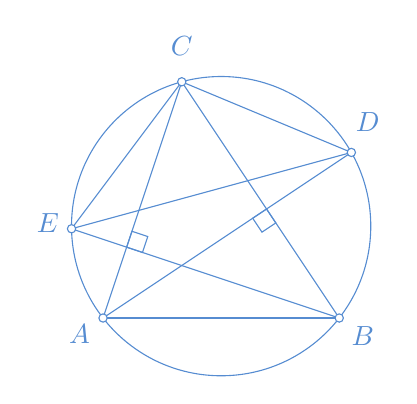
\begin{tikzpicture}[cackithi]
			\draw (0.9004185552987112,2.2669457035324743) -- (1.0180882363816217,2.0904411819081083) -- (1.1945927580059874,2.208110862991019) -- (1.0769230769230769,2.3846153846153846) -- cycle; 
			\draw (-0.4987538820250189,1.8329179606750063) -- (-0.4316718427000252,2.0341640786499875) -- (-0.6329179606750064,2.101246117974981) -- (-0.7,1.9) -- cycle; 
			\draw  (0.5,2.1666666666666665) circle (1.9002923751652299cm);
			\draw  (-1.,1.)-- (2.,1.);
			\draw  (2.,1.)-- (0.,4.);
			\draw  (0.,4.)-- (-1.,1.);
			\draw  (-1.,1.)-- (2.1538461538461533,3.102564102564102);
			\draw  (2.,1.)-- (-1.4,2.1333333333333333);
			\draw  (-1.4,2.1333333333333333)-- (2.1538461538461533,3.102564102564102);
			\draw  (2.1538461538461533,3.102564102564102)-- (0.,4.);
			\draw  (0.,4.)-- (-1.4,2.1333333333333333);
				\draw [fill=white] (-1.,1.) circle (1.5pt);
				\draw (-1.3,0.79) node {$A$};
				\draw [fill=white] (2.,1.) circle (1.5pt);
				\draw (2.3,0.77) node {$B$};
				\draw [fill=white] (0.,4.) circle (1.5pt);
				\draw (0.,4.45) node {$C$};
				\draw [fill=white] (2.1538461538461533,3.102564102564102) circle (1.5pt);
				\draw (2.36,3.49) node {$D$};
				\draw [fill=white] (-1.4,2.1333333333333333) circle (1.5pt);
				\draw (-1.7,2.21) node {$E$};
		\end{tikzpicture}
		\vspace*{-10pt}
	\end{figure}
	Do $ABC$ là tam giác nhọn nên các điểm $D$ và $E$ lần lượt nằm ở bên trong cung nhỏ $BC$ và $AC$ như trong hình vẽ. Như vậy $\angle ECD$ lớn hơn  $\angle ACB$. Từ giả thiết $AB=DE,$ ta có $\angle ECD= 180^\circ - \angle ACB$.  \hfill ($1$)
	\vskip 0.1cm
	Mặt khác ta có
	\begin{align*}
		\angle ECD =\,&\angle ECA + \angle ACB + \angle BCD \\
		= \,&\angle EBA + \angle ACB + \angle BAD \\
		= \,&90^\circ \!\!-\!\! \angle BAC \!\!+\!\! \angle ACB \!\!+\!\! 90^\circ \!\!-\!\! \angle ABC \\
		= \,&(180^\circ \!-\! \angle BAC \!-\! \angle ABC) \!+\! \angle ACB  \\
		= \,&2\angle ACB  \tag{$2$}
	\end{align*}
	Từ ($1$) và ($2$) ta nhận được điều cần chứng minh.
	\vskip 0.1cm
	{\bf\color{cackithi} OC$\pmb{26.}$} Giả sử bạn có vô hạn các hình chữ $T$ (bao gồm bốn hình vuông cạnh
	$1$) như trong hình vẽ, và một bảng ô vuông cỡ $n \times n.$ Bạn được phép đặt một số hình trên bảng (có thể xoay chúng), miễn là không có hai hình nào chồng lên nhau và không có hình nào vượt ra khỏi bảng.
	\vskip 0.1cm
	Với những giá trị nào của $n$ thì bạn có thể phủ toàn bộ bảng?
	\begin{figure}[H]
		\vspace*{-5pt}
		\centering
		\captionsetup{labelformat= empty, justification=centering}
		\begin{tikzpicture}[cackithi,scale=0.88]
			\draw (0,0) grid (3,1);
			\draw (1,-1) grid (2,0);
		\end{tikzpicture}
		\vspace*{-10pt}
	\end{figure}
	\textit{Lời giải.} Trước tiên ta nhận thấy mỗi hình chữ $T$ gồm $4$ ô, do đó nếu phủ kín được bảng thì diện tích của bảng phải chia hết cho $4$, tức là $n$ chẵn.
	\vskip 0.1cm
	Với $n$ chia hết cho $4$ ta có thể chia bảng thành các bảng con cỡ $4\times 4$ và phủ kín mỗi bảng con bằng $4$ hình chữ $T$ như sau:
	\begin{figure}[H]
		\vspace*{-5pt}
		\centering
		\captionsetup{labelformat= empty, justification=centering}
		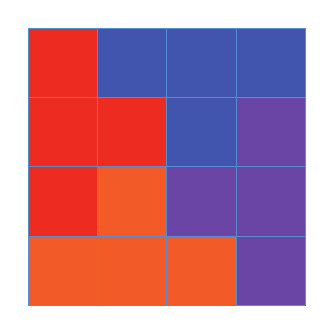
\begin{tikzpicture}[cackithi,scale=0.88]
			\filldraw[duongvaotoanhoc] (0,0) rectangle (3,1);
			\filldraw[gocco] (3,0) rectangle (4,3);
			\filldraw[timhieukhoahoc] (4,3) rectangle (1,4);
			\filldraw[toanhocdoisong] (0,1) rectangle (1,4);
			\filldraw[duongvaotoanhoc] (1,1) rectangle (2,2);
			\filldraw[gocco] (2,1) rectangle (3,2);
			\filldraw[timhieukhoahoc] (2,2) rectangle (3,3);
			\filldraw[toanhocdoisong] (1,2) rectangle (2,3);
			\draw (0,0) grid (4,4);
		\end{tikzpicture}
		\vspace*{-10pt}
	\end{figure}
	Với $n=4k+2,$ ta tô màu đen, trắng các ô trong bảng như bàn cờ vua. Để lát kín bảng cần tất cả $\dfrac{n^2}{4}=(2k+1)^2$ hình chữ $T$. Như vậy có một số lẻ hình chữ $T$ và mỗi hình phủ $1$ hoặc $3$ ô đen, tức là tổng số ô đen phải là lẻ. Nhưng thực tế có  $\dfrac{n^2}{2}=2(2k+1)^2$ ô đen. Do đó trường hợp này không thể phủ kín bảng như yêu cầu. 
	\begin{figure}[H]
		\vspace*{-5pt}
		\centering
		\captionsetup{labelformat= empty, justification=centering}
		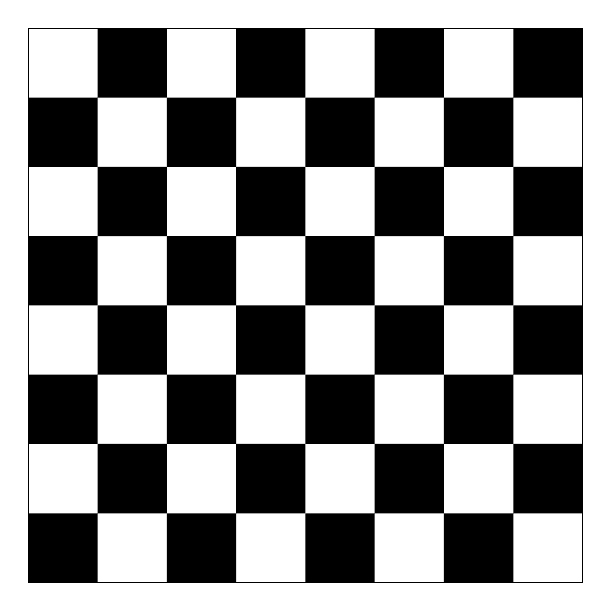
\begin{tikzpicture}[scale=0.88]
			\draw (0,0) rectangle (8,8);
			\foreach \y in {0,2,...,6}{
				\foreach \x in {0,2,...,6}{
					\fill (\x,\y) rectangle (1+\x,1+\y) rectangle (2+\x,2+\y);}}
		\end{tikzpicture}
		\vspace*{-5pt}
	\end{figure}
	Tóm lại ta phủ kín được bảng bằng các hình chữ $T$ khi và chỉ khi $n$ chia hết cho $4$.
	\vskip 0.1cm
	{\bf\color{cackithi} OC$\pmb{27.}$} Giả sử rằng các số thực $a$ và $b$ thỏa mãn
	\begin{align*}
		ab+ \sqrt{ab+1} +\sqrt{a^2+b}\ \sqrt{b^2+a}=0.
	\end{align*}
	Tìm giá trị của biểu thức
	\begin{align*}
		S=a\sqrt{b^2+a} + b\sqrt{a^2+b}.
	\end{align*}
	\textit{Lời giải.} Từ đẳng thức trong bài, chuyển vế và bình phương hai vế ta có
	\begin{align*}
		& \ ab+ \sqrt{a^2+b} \sqrt{b^2+a} = \sqrt{ab+1} \\
		\Rightarrow\  &	a^2b^2 + 2ab\sqrt{a^2+b} \sqrt{b^2+a} \\
		&+ (a^2+b)(b^2+a) = ab+1\\
		\Leftrightarrow\  &	(a^2b^2+a^3) + 2ab\sqrt{a^2+b} \sqrt{b^2+a} \\
		&+ (b^3+a^2b^2) = 1\\
		\Leftrightarrow\ 	& (a\sqrt{b^2+a} + b\sqrt{a^2+b})^2 = 1.
	\end{align*}
	Ta nhận được $S=\pm 1.$ Ta sẽ chứng minh $S$ luôn dương. Thực vậy, từ giả thiết ta có
	\begin{align*}
		ab= -\sqrt{ab+1} -\sqrt{a^2+b} \sqrt{b^2+a} <0.
	\end{align*}
	Không mất tổng quát, ta có thể giả sử \linebreak $a>0>b.$ Khi đó, do $a>\sqrt{a^2+b},$ ta có
	\begin{align*}
		S= a( \sqrt{b^2+a} +b)- b(a- \sqrt{a^2+b})>0.
	\end{align*} 
	Do đó  $S=1$.
	\vskip 0.1cm
	Trong phần cuối của chuyên mục kỳ này, chúng tôi sẽ giới thiệu với bạn đọc ba bài toán trong kỳ thi Olympic Toán học trẻ khối Pháp ngữ năm $2022$. Các bài toán này phù hợp với trình độ học sinh năm cuối cấp Trung học cơ sở.
	\vskip 0.1cm
	{\bf\color{cackithi} OC$\pmb{34.}$} Tìm tất cả các số nguyên dương $n$ sao cho $ \lfloor \sqrt{n}\rfloor $ là ước của $n.$ 
	\vskip 0.1cm
	\textit{Chú ý}: $ \lfloor x \rfloor $ ký hiệu phần nguyên của một số thực $x,$ được định nghĩa là số nguyên lớn nhất nhỏ hơn hoặc bằng $x.$ Ví dụ: $ \lfloor 1.4 \rfloor =1$, $ \lfloor 2 \rfloor=2,$ và  $ \lfloor 2.9 \rfloor= 2.$  
	\vskip 0.1cm
	{\bf\color{cackithi} OC$\pmb{35.}$} Cho một bảng ô vuông cỡ $n \times n$ với $n\ge 1$. Aya muốn tô màu  $k$ ô của bảng  sao cho chỉ có duy nhất một cách để đặt  $n$ đồng xu trên các ô vuông được tô màu sao cho không có hai đồng xu nào nằm trên cùng một hàng hoặc cột. Hỏi giá trị tối đa có thể của $k$  là bao nhiêu?
	\vskip 0.1cm
	{\bf\color{cackithi} OC$\pmb{36.}$} Cho tam giác $ABC$ và $D$ là giao điểm của đường phân giác của góc $\angle BAC$ và đường trung trực của cạnh $AC$. Đường thẳng  đi qua $B$ và song song với $AC$, cắt đường thẳng $AD$ tại $X$. Đường thẳng đi qua $B$ và song song với $CX$, cắt đường thẳng $AC$ tại $Y$. Đường tròn ngoại tiếp tam giác $ABY$ cắt đường thẳng $BX$ tại $E.$ Chứng minh rằng ba điểm $C$ , $D$ và $E$ thẳng hàng.
\end{multicols}
%	\newpage
%
%	\setcounter{figure}{0}
%	\thispagestyle{timhieukhoahocnone}
\pagestyle{timhieukhoahoc}
\everymath{\color{timhieukhoahoc}}
\blfootnote{$^1$\text{\color{timhieukhoahoc}Nguồn: Tia Sáng https://tiasang.com.vn/khoa-hoc-cong-nghe/nobel-y-hoc-2022-ky-cuoi-tai-sao-loai-nguoi-song-sot/.}}
\graphicspath{{../timhieukhoahoc/pic/}}
\begingroup
\AddToShipoutPicture*{\put(0,616){\includegraphics[width=19.3cm]{../bannertimhieu}}}
\AddToShipoutPicture*{\put(110,550){\includegraphics[scale=1]{../tieude2.pdf}}}
\centering
\endgroup
\vspace*{155pt}

\begin{multicols}{2}
	Vườn thú Leipzig nằm ở bên kia rìa thành phố so với Viện Nhân chủng học Tiến hóa. Nhưng viện này có phòng thí nghiệm riêng trong khuôn viên, cũng như các phòng thử nghiệm được thiết kế đặc biệt bên trong ngôi nhà nghiên cứu về vượn, được gọi là Pongoland. Vì không ai trong số họ hàng Neanderthal gần nhất của chúng ta sống sót (ngoại trừ những mảnh DNA nhỏ trong chúng ta), các nhà nghiên cứu phải dựa vào họ hàng gần nhất của chúng ta là tinh tinh và bonobos, hay họ hàng xa hơn là khỉ đột và đười ươi -- để thực hiện các thí nghiệm sống. Một buổi sáng, tôi đến sở thú hy vọng sẽ xem một thí nghiệm đang được tiến hành.
	\begin{figure}[H]
		\vspace*{-5pt}
		\centering
		\captionsetup{labelformat= empty, justification=centering}
		\includegraphics[width= 1\linewidth]{4}
		\caption{\small\textit{\color{timhieukhoahoc}Nhiều dữ liệu khảo cổ học đã hé lộ phần nào đời sống thường ngày của người Neanderthal hàng chục nghìn năm trước. Ảnh: mpg.de}}
		\vspace*{-10pt}
	\end{figure}
	Để lên hình cho đẹp, một nhà nghiên cứu tên là Héctor Marín Manrique chuẩn bị thực hiện lại một loạt các thí nghiệm khoa học mà ông đã làm. Một con đười ươi cái tên là Dokana được dẫn vào một trong những phòng thử nghiệm. Giống như hầu hết các con đười ươi khác, nó có bộ lông màu đồng và vẻ ngoài khinh khỉnh. Trong thí nghiệm đầu tiên liên quan đến nước trái cây màu đỏ và các ống nhựa nhỏ, Dokana có thể phân biệt ống hút nào thì dùng được và ống hút nào thì không. Trong phần thứ hai, có nhiều nước màu đỏ hơn và nhiều nhựa hơn, nó hiểu ý tưởng về ống hút bằng cách ngắt một đoạn của đường ống và dùng ống đó để hút nước. Cuối cùng, trong một màn thể hiện tài khéo léo ở cấp độ IQ cao thể hiện trí thông minh của loài vượn lớn, Dokana đã lấy được một hạt đậu phộng mà Manrique đã đặt ở đáy của một ống trụ dài. (Hình trụ được gắn cố định vào tường nên không thể dốc ngược ra). Nó đi đến chỗ uống nước, ngậm một ít nước trong miệng, trở lại và nhổ vào hình trụ, lặp lại quá trình cho đến khi hạt đậu phộng nổi đến tầm với của mình. Về sau, tôi thấy thí nghiệm này được dàn dựng lại với một số trẻ em năm tuổi sử dụng các hộp nhựa nhỏ hơn, những hạt đậu phộng được thay bằng kẹo. Mặc dù một bình đầy nước đã cố tình được để gần đó nhưng chỉ có một đứa trẻ -- một bé gái -- nghĩ ra phương án làm nó nổi lên và cũng phải sau một hồi gợi ý đủ kiểu (có bé trai còn hỏi “Nước thì giúp con kiểu gì?”, ngay trước khi bỏ cuộc).
	\vskip 0.1cm
	Một cách để cố gắng trả lời câu hỏi “Điều gì làm nên con người chúng ta?” là hỏi “Điều gì khiến chúng ta khác với loài vượn?” hoặc, nói chính xác hơn, với loài vượn khác (vì con người cũng thuộc nhóm vượn). Như tất cả mọi người giờ đây đã biết -- và như các thí nghiệm với Dokana một lần nữa khẳng định -- loài vượn khác cực kỳ thông minh. Chúng có khả năng suy luận, giải các câu đố phức tạp và hiểu những gì người khác có thể biết và không biết. Khi các nhà nghiên cứu từ Leipzig thực hiện một loạt các thử nghiệm trên tinh tinh, đười ươi và những đứa trẻ hai tuổi rưỡi, họ phát hiện ra rằng tinh tinh, đười ươi và những đứa trẻ khá tương đồng với nhau trong một loạt các hoạt động liên quan đến việc tìm hiểu về thế giới vật chất. Ví dụ: nếu một người thử nghiệm đặt phần thưởng vào một trong ba chiếc cốc, rồi tráo vị trí ba cốc này, thì loài vượn tìm ra phần thưởng cũng giỏi như lũ trẻ -- thậm chí, trong trường hợp của tinh tinh, còn giỏi hơn. Những con vượn dường như nắm bắt được khái niệm về số lượng tốt như lũ trẻ -- chúng luôn chọn chiếc đĩa chứa nhiều món hơn, thậm chí việc lựa chọn này cần dựa trên kỹ năng mà ta có thể tạm gọi là toán học -- và dường như loài vượn cũng nắm bắt tốt không kém bọn trẻ về quan hệ nhân quả. (Ví dụ, loài vượn hiểu rằng khi lắc một chiếc cốc mà chúng kêu lạo xạo thì khả năng cốc đó có thức ăn là cao hơn những chiếc cốc không phát ra tiếng động nào.) Và chúng cũng khôn khéo không thua gì trẻ em trong việc tận dụng các công cụ đơn~giản.
	\vskip 0.1cm
	Tuy nhiên, những đứa trẻ vượt trội hơn những con vượn ở điểm đọc các tín hiệu xã hội. Khi bọn trẻ được gợi ý về nơi tìm phần thưởng -- ai đó chỉ vào hoặc nhìn vào đúng hộp đựng -- lũ trẻ sẽ nhanh chóng bắt lấy cơ hội. Những con vượn thì hoặc là không hiểu chúng đang được giúp đỡ một tay, hoặc là không thể làm theo gợi ý. Tương tự, khi bọn trẻ được chỉ cách lấy phần thưởng, chẳng hạn như bằng cách xé toang hộp, chúng hiểu ý ngay và làm theo. Lũ vượn, một lần nữa, hết sức lúng túng. Phải thừa nhận rằng bọn trẻ có lợi thế lớn trong các hành động liên quan đến tương tác xã hội, vì chính những người thiết kế thí nghiệm cũng cùng giống loài với các em. Nhưng, nói chung, vượn dường như không có nhiều động lực để đạt được kỹ năng hợp tác cùng giải quyết vấn đề, vốn là trọng tâm của xã hội loài người.
	\vskip 0.1cm
	Michael Tomasello, người đứng đầu bộ phận tâm lý học so sánh và phát triển của viện, nói với tôi: “Tinh tinh làm nhiều điều cực kỳ thông minh. Nhưng sự khác biệt chính [giữa con người và chúng] mà chúng tôi thấy là kỹ năng ‘ba cây chụm lại nên hòn núi cao’. Giờ đây nếu bạn quan sát ở sở thú, bạn sẽ không bao giờ thấy hai con tinh tinh cùng nhau khiêng vật nặng. Chúng không có kiểu hoạt động hợp tác như vậy”.
	\begin{figure}[H]
		\vspace*{-5pt}
		\centering
		\captionsetup{labelformat= empty, justification=centering}
		\includegraphics[width= 1\linewidth]{5}
		\caption{\small\textit{\color{timhieukhoahoc}Hang động Grotte des Combarelles trên vách tràn ngập các bức vẽ của người tối cổ. Điều gì thôi thúc con người len lỏi trong bóng tối mịt mù và chật hẹp để tạo nên những tác phẩm chưa chắc đã có người đồng cảm? Ảnh: National Geographic.}}
		\vspace*{-10pt}
	\end{figure}
	Trở về từ sở thú, tôi hỏi Pääbo về một thí nghiệm giả định. Nếu ông có cơ hội khiến người Neanderthal phải trải qua các loại bài kiểm tra mà tôi đã thấy ở Pongoland, ông sẽ làm gì? Ông ấy có nghĩ rằng mình có thể nói chuyện với họ không? Ông ngả người ra sau ghế và khoanh tay trước ngực.
	\vskip 0.1cm
	“Ai cũng không kìm được sự tò mò,” ông nói. “Vì vậy, tôi cố gắng kiềm chế điều đó bằng cách từ chối các câu hỏi như: ‘Họ có biết nói không?’ Bởi vì, thực sự thì tôi không biết trả lời thế nào, và theo một cách nào đó, tôi cũng chỉ biết suy đoán như bạn mà thôi”.
	\vskip 0.1cm
	Cho đến nay, rất nhiều địa điểm của người Neanderthal đã được khai quật, từ miền Tây Tây Ban Nha đến miền Trung nước Nga và từ Israel đến xứ Wales. Chúng cung cấp nhiều manh mối về người Neanderthal trông ra sao, ít nhất là với những người thích suy đoán. Người Neanderthal cực kỳ mạnh mẽ -- điều này được chứng thực bởi độ dày của xương họ -- và có thể đánh chúng ta nhừ tử cũng nên. Họ rất thành thạo trong việc chế tạo công cụ bằng đá, mặc dù có vẻ họ dành ra hàng chục nghìn năm chỉ để làm đi làm lại một vài công cụ, với những thay đổi không đáng kể. Ít nhất là trong một số trường hợp, họ chôn cất người đã khuất. Nhưng cũng trong một số trường hợp khác, họ có vẻ còn giết và ăn thịt lẫn nhau. Những vết nứt vỡ trên răng cửa của họ cho thấy họ đã rất mất công để dùng răng ngoạm da động vật, và điều này cũng gợi ý rằng họ đã xử lý da đó thành một loại da thuộc. Bộ xương của người Neanderthal thường để lại nhiều dấu vết của bệnh tật hoặc biến dạng. Ví dụ như người Neanderthal ban đầu của Mettmann, dường như đã phải trải qua và hồi phục từ hai vết thương nghiêm trọng, một ở đầu và một ở cánh tay trái. Người Neanderthal có bộ xương gần như hoàn chỉnh được tìm thấy ở La Chapelle đã phải chịu đựng ngoài việc bị viêm khớp còn bị gãy xương sườn và xương bánh chè ở đầu gối. Cả hai cá nhân này đều sống qua tuổi năm mươi, điều này cho thấy rằng người Neanderthal có khả năng hành động tập thể, hay nói cách khác mĩ miều hơn là có sự thấu cảm. Họ phải -- ít nhất là cũng có khi -- chăm sóc vết thương của đồng loại.
	\vskip 0.1cm
	Từ các nghiên cứu khảo cổ học, người ta suy ra rằng người Neanderthal tiến hóa ở châu Âu hoặc tây Á và tỏa đi từ đó, chỉ dừng chân ở thủy vực hoặc gặp phải những trở ngại đáng kể nào đó khác. (Trong thời kỳ băng hà, mực nước biển thấp hơn rất nhiều so với hiện tại, vì vậy không có eo biển Anh để vượt qua). Đây là một trong những điểm cơ bản nhất mà con người hiện đại khác với người Neanderthal và, theo quan điểm của Pääbo, cũng là một trong những điều lý thú nhất. Vào khoảng bốn mươi lăm nghìn năm trước, con người hiện đại đã đặt chân đến Úc, một cuộc hành trình, kể cả ở giữa kỷ băng hà, cũng có nghĩa là băng qua vùng nước mở. Những con người cổ đại như Homo erectus “chỉ đi loanh quanh như rất nhiều loài động vật có vú khác ở thời Cựu Thế giới,” Pääbo nói với tôi. “Họ không bao giờ đến Madagascar, không bao giờ đến Úc. Người Neanderthal cũng vậy. Chỉ có những con người hoàn toàn hiện đại mới bắt đầu hành trình mạo hiểm trên đại dương, nơi người ta không nhìn thấy đất liền. Tất nhiên, một phần là nhờ công nghệ; bạn phải có tàu để làm điều đó. Nhưng tôi thích nghĩ và nói rằng, còn cần một chút “điên rồ” nữa. Bạn biết không, biết bao nhiêu người hẳn đã ra khơi và biến mất trên Thái Bình Dương trước khi đặt chân được đến đảo Phục Sinh? Ý tôi là, điều đó thật nực cười. Và tại sao người ta lại dám làm thế? Có phải vì vinh quang? Vì sự bất tử? Vì tò mò? Giờ đây chúng ta còn đòi lên sao Hỏa nữa. Đúng là không biết điểm dừng”. Nếu đặc tính của con người hiện đại là sự thao thức, “không bao giờ bằng lòng với hiện tại” của nhân vật Faust trong vở kịch của Geothe, hẳn phải có một loại gene Faust nào đó trong chúng ta, theo quan điểm của Pääbo. Rất nhiều lần, ông nói với tôi rằng có thể xác định được nguyên nhân của sự “điên rồ” này bằng cách so sánh DNA của Neanderthal và con người.
	\vskip 0.1cm
	“Nếu một ngày nào đó chúng ta biết được rằng một số đột biến kỳ lạ đã làm nên sự điên rồ và thích khám phá mọi thứ của con người, thì sẽ thật ảo diệu khi nghĩ rằng chỉ một chút xáo trộn này trên nhiễm sắc thể kia mà đã tạo nên ngày hôm nay, đã thay đổi toàn bộ hệ sinh thái trên hành tinh này và khiến chúng ta thống trị tất cả”.
	\vskip 0.2cm
	\PIbox{Nếu đặc tính của con người hiện đại là sự thao thức, “không bao giờ bằng lòng với hiện tại” của nhân vật Faust trong vở kịch của Geothe, hẳn phải có một loại gene Faust nào đó trong chúng ta, theo quan điểm của Pääbo.}
	\vskip 0.2cm
	Theo những ước tính gần đây nhất, người Neanderthal và người hiện đại có chung một tổ tiên sống cách đây khoảng bốn trăm nghìn năm. (Không rõ tổ tiên đó là ai, mặc dù có một khả năng là loài hominid nào đó mới được biết đến một cách mơ hồ, sau khi người ta tìm thấy một xương hàm ở gần Heidelberg, với tên gọi Homo heidelbergensi). Còn tổ tiên chung của tinh tinh và người, sống cách đây năm đến bảy triệu năm trước. Điều này có nghĩa là người Neanderthal và con người có ít hơn $1/10$ thời gian đó để tích lũy sự khác biệt về gene.
	\begin{figure}[H]
		\vspace*{-5pt}
		\centering
		\captionsetup{labelformat= empty, justification=centering}
		\includegraphics[width= 1\linewidth]{6}
		\caption{\small\textit{\color{timhieukhoahoc}Người ta cần khoảng $400$ mg bột xương để thực hiện một phân tích gene. Nhưng nhiều khi kết quả không chỉ gồm gene của người Neanderthal mà còn tạp nhiễm cả của vi sinh vật. Ảnh: mpg.de}}
		\vspace*{-10pt}
	\end{figure}
	Về nguyên tắc, việc lập bản đồ những khác biệt này khá đơn giản về lý thuyết. Còn trong thực tế, nó phức tạp hơn một chút. Để bắt đầu, thực sự không có cái gọi là bộ gene chung của con người; ai cũng có bộ gene của riêng mình và chúng khác nhau đáng kể -- giữa bạn và người ngồi cạnh bạn trên tàu điện ngầm, sự khác biệt rất có thể là đâu đó khoảng ba triệu cặp cơ bản. Một số biến thể này tương ứng với những khác biệt sinh lý có thể nhìn thấy -- chẳng hạn như màu mắt, hoặc khả năng mắc bệnh liên quan đến tim mạch -- và một số khác không có ý nghĩa đáng kể. Theo ước tính đầu tiên, một người và một người Neanderthal bất kỳ cũng sẽ khác nhau ba triệu cặp cơ sở. Cái khó là xác định chắc chắn cái nào trong số hàng triệu biến thể này đã tách chúng ta khỏi họ. Pääbo ước tính rằng khi Dự án bộ gene người Neanderthal hoàn thành, danh sách các cặp cơ bản độc nhất của con người với người Neanderthal sẽ đâu đó khoảng một trăm nghìn cặp. Đâu đó trong danh sách này sẽ ẩn giấu sự thay đổi -- hay những thay đổi -- đã khởi tạo nên chúng ta. Để xác định những đột biến gene này, ông cần phải nhờ đến những con chuột chuyển~gene.
	\vskip 0.1cm
	Từ quan điểm thực nghiệm, cách tốt nhất để kiểm tra xem thay đổi gene nào mới đáng kể là tạo ra một con người với trình tự gene của người Neanderthal. Điều này sẽ liên quan đến việc chỉnh sửa tế bào gốc của người, cấy phôi đã biến đổi gene đó vào một phụ nữ mang thai hộ và rồi quan sát đứa trẻ của thí nghiệm đó lớn lên. Vì những lý do quá rõ ràng, không ai cho phép một thí nghiệm trên người như vậy, đó còn chưa kể là nó còn bất khả. Vì những lý do tương tự, thí nghiệm kiểu này cũng không được phép áp dụng trên tinh tinh. Nhưng trên chuột thì được. Hàng chục giống chuột đã được chỉnh sửa gene để mang các trình tự gene của người, và người ta vẫn tạo ra các giống mới liên tục, đặt hàng khá dễ dàng.
	\vskip 0.1cm
	Vài năm trước, Pääbo và một đồng nghiệp, Wolfgang Enard, bắt đầu quan tâm đến một gene được gọi là FOXP$2$, gene này ở người có liên quan đến ngôn ngữ. (Những người có một bản sao gene bị lỗi -- một trường hợp cực kỳ hiếm xảy ra -- có khả năng nói, nhưng những gì họ nói, đối với người lạ, hầu như không thể hiểu được.) Pääbo và Enard đã nuôi một số con chuột với một phiên bản gene này, và sau đó nghiên cứu chúng từ mọi góc độ có thể. Những con chuột bị biến đổi, có giọng kêu trầm hơn so với các đồng loại chưa được “nhân hóa” của chúng. Những con chuột này cũng thể hiện sự khác biệt đáng kể về phát triển thần kinh. Gene FOXP$2$ của người Neanderthal, hóa ra, gần như giống hệt loài người, khác có mỗi một cặp base. Khi ông phát hiện ra sự khác biệt này, ông đặt hàng ngay một lô chuột chuyển gene mới mà lúc tôi tới thăm phòng thí nghiệm của ông, vừa mới sinh ra và đang được nuôi trong điều kiện tiệt trùng dưới tầng hầm.
	\vskip 0.1cm
	Các gene liên quan đến kỹ năng nói của chúng ta là địa chỉ hiển nhiên để tìm kiếm những thay đổi khiến chúng ta là con người. Nhưng lý do của việc phải giải trình tự toàn bộ hệ gene của người Neanderthal là bởi địa chỉ hiển nhiên nhất chưa chắc đã là địa chỉ đúng nhất.
	\vskip 0.1cm
	Pääbo nói với tôi: “Ưu điểm tuyệt vời của nghiên cứu gene theo phương thức này là nó không có thiên kiến. Nếu bạn chỉ chạy theo những gene ứng cử viên, bạn sẽ dễ phát biểu cảm tính rằng gene này hay gene kia mới là quan trọng nhất. Nhiều người sẽ bảo là gene ngôn ngữ. Nhưng có khi chúng ta sẽ ngạc nhiên vì gene khác mới là cốt yếu”. Gần đây, Pääbo trở nên hứng thú với một gene có tên là RUNX$2$, liên quan đến quá trình hình thành xương. Khi các thành viên trong nhóm của ông phân tích toán học bộ gene người và người Neanderthal, RUNX$2$ bỗng nổi lên như một vị trí đánh dấu sự rẽ nhánh của những dòng dõi người.
	\vskip 0.1cm
	Những người có bản sao bị lỗi của gene RUNX$2$ thường phát triển một tình trạng, được gọi là chứng loạn sản xương sọ, có các triệu chứng bao gồm các đặc điểm bề ngoài giống người Neanderthal như khung xương sườn loe ra. Hai gene có liên quan đến chứng tự kỷ, CADPS$2$ và AUTS$2$, dường như có sự khác biệt đáng kể giữa người Neanderthal và người. Điều này rất thú vị vì một trong những triệu chứng của chứng tự kỷ là không có khả năng đọc các tín hiệu xã hội.
	\vskip 0.1cm
	Vào một buổi chiều nọ, khi tôi đi lang thang trong văn phòng của ông, Pääbo cho tôi xem một bức ảnh chụp nắp sọ mới được một nhà sưu tập nghiệp dư phát hiện cách Leipzig khoảng nửa giờ. Từ bức ảnh đã được gửi qua email, Pääbo nhận định rằng chiếc xương sọ có thể là đồ cổ -- từ thời sơ khai của người Neanderthal, hoặc thậm chí là người Homo heidelbergensis. Ông cũng quyết định phải có nó bằng được. Chiếc nắp sọ đã được tìm thấy tại một mỏ đá trong một hố nước -- ông giả thiết rằng có lẽ những điều kiện này đã bảo quản nó, và nếu ông nhanh chóng kịp đưa nó về, ông có thể trích xuất một số DNA. Nhưng hộp sọ đã được hứa đưa tới một giáo sư nhân chủng học ở Mainz trước. Làm thế nào mà Pääbo thuyết phục người giáo sư để lại cho ông đủ xương để kiểm nghiệm bây~giờ?
	\vskip 0.1cm
	Pääbo gọi cho tất cả những người mà ông nghĩ biết đâu có thể quen với giáo sư kia. Ông còn yêu cầu thư ký của mình liên hệ với thư ký của giáo sư kia để xin số điện thoại cá nhân và nói đùa -- có khi nửa đùa nửa thật cũng nên -- rằng nếu cần thiết thì Pääbo sẵn sàng “bán thân” cho giáo sư luôn. Cuộc gọi điện thoại qua lại điên cuồng trên khắp nước Đức kéo dài hơn một tiếng rưỡi đến khi cuối cùng Pääbo quay ra nói chuyện với một nhà nghiên cứu cùng lab với mình. Nhà nghiên cứu này hóa ra đã tận mắt nhìn thấy chiếc nắp sọ thực sự và kết luận miếng xương này khả năng cao là không phải đồ cổ gì cho lắm. Pääbo ngay lập tức không còn hứng thú gì với nó nữa.
	\vskip 0.1cm
	Với những bộ xương cổ, không ai thực sự biết trước có thể thu được thông tin gì từ nó. Cách đây vài năm, Pääbo lấy được một phần răng từ một trong những bộ xương được gọi là “người Hobbit” được tìm thấy trên đảo Flores, Indonesia. (“Người Hobbit”, được phát hiện vào năm $2004$, thường được cho là loài người cổ đại thấp bé -- Homo floresiensis -- mặc dù một số nhà khoa học đã lập luận rằng đó chỉ là người hiện đại bị chứng teo não.) Chiếc răng, khoảng $17$ nghìn tuổi, không chứa một chút DNA nào.
	\vskip 0.1cm
	Sau đó, khoảng một năm rưỡi trước, Pääbo đã lấy được một mảnh xương ngón tay được khai quật trong một hang động ở miền Nam Siberia cùng với một chiếc răng hàm kỳ dị, trông có vẻ giống người. Xương ngón tay -- có kích thước bằng cục tẩy bút chì -- được cho là đã hơn bốn vạn năm tuổi. Pääbo cho rằng nó đến từ người hiện đại hoặc từ người Neanderthal. Nếu điều này là đúng, thì địa điểm đó sẽ là nơi xa nhất về phía Đông mà người ta tìm thấy hài cốt người Neanderthal.
	\vskip 0.1cm
	Trái ngược với chiếc răng của người Hobbit, đoạn ngón tay mang lại một lượng DNA lớn đáng kinh ngạc. Khi việc phân tích các mẩu thông tin đầu tiên được hoàn thành, Pääbo tình cờ lúc đó đang ở Hoa Kỳ. Ông gọi điện đến văn phòng và một trong những đồng nghiệp của ông trả lời: “Ông đang ngồi chắc chắn trên ghế chứ?” DNA cho thấy dữ liệu không thể thuộc về người Neanderthal hoặc của người hiện đại. Thay vào đó, chủ nhân của nó phải thuộc về một loài hominid hoàn toàn khác và chưa từng được phát hiện ra trước đó. Trong một bài báo được xuất bản vào tháng $12/2010$, trên tạp chí Nature, Pääbo và nhóm của ông đã đặt tên cho nhóm này là người Denisovan, theo tên của hang Denisova, nơi xương đã được tìm thấy. Tờ \textit{Sydney Morning Herald} chạy tít: “Một ngón tay đóng dấu lịch sử cổ đại của con người”. Thật đáng kinh ngạc -- hay có lẽ, giờ đây, người ta cũng đã đoán được -- con người hiện đại hẳn đã phối ngẫu với cả người Denisovan bởi vì những người New Guinean ngày nay mang tới $6\%$ DNA của người Denisovan. (Tại sao điều này đúng với người New Guinea nhưng không phải với người Siberia bản địa hoặc người châu Á thì chưa rõ, nhưng có lẽ liên quan đến các mẫu hình di cư của con người).
	\vskip 0.1cm
	Từ lâu, người ta đã hiểu rằng con người hiện đại và người Neanderthal là những người sống cùng thời với nhau. Việc phát hiện ra người Hobbit và bây giờ là người Denisovan cho thấy con người đã chia sẻ hành tinh với ít nhất hai sinh vật khác giống như chúng ta. Và có vẻ như càng phân tích DNA từ các bộ hài cốt cổ đại thì sẽ càng thấy những loài khác có họ hàng với người; như Chris Stringer, một nhà cổ sinh vật học nổi tiếng người Anh, đã nói với tôi, “Tôi chắc chắn rằng chúng ta sẽ có thêm nhiều điều bất ngờ nữa đang đến.”
	\vskip 0.1cm
	“Nếu những dạng người khác này tồn tại được hơn hai nghìn thế hệ nữa, tức là không quá lâu, thì điều đó sẽ ảnh hưởng như thế nào đến quan điểm của chúng ta về thế giới sinh vật?” Pääbo nói, khi sự phấn khích với câu chuyện về xương nắp sọ đã chùng xuống và chúng tôi ngồi uống cà phê với nhau. “Chúng ta từng đặt ra một ranh giới rõ ràng giữa con người và động vật. Nhưng có thể ranh giới đó không rõ ràng đến thế. Đó là một điều thú vị để triết lý.” Cũng thật thú vị khi nghĩ về lý do tại sao chúng ta là những người sống sót.
	\vskip 0.1cm
	Trong nhiều thập kỷ, nhiều giả thuyết đã được đưa ra để giải thích nguyên nhân gây ra sự diệt vong của người Neanderthal, từ biến đổi khí hậu cho đến vận rủi đơn thuần. Tuy nhiên, trong những năm gần đây, ngày càng rõ ràng rằng, như Pääbo đã nói với tôi, “vận rủi của họ là chính chúng ta”. Hết lần này đến lần khác, bằng chứng khảo cổ học ở châu Âu chỉ ra rằng, mỗi khi con người hiện đại xuất hiện ở nơi nào người Neanderthal đang sinh sống, thì người Neanderthal ở vùng đó sẽ biến mất. Có thể người Neanderthal đã bị truy đuổi ráo riết, hoặc có lẽ họ đã bị thua trong cuộc cạnh tranh sinh tồn. “Vận rủi” của người Neanderthal có lẽ giống với bất hạnh mà người Hobbit và người Denisovan gặp phải, và tương tự như thảm kịch mà các loài thú có túi khổng lồ từng thống trị khắp Australia, và một loạt các loài thú lớn từng sinh sống ở Bắc Mỹ, những con chim Moa từng sống ở New Zealand. Và chính sự xui xẻo đó đã đưa rất nhiều loài -- trong đó có tất cả các loài vượn lớn -- đến bờ vực của sự lãng quên ngày nay.
	\begin{figure}[H]
		\vspace*{-5pt}
		\centering
		\captionsetup{labelformat= empty, justification=centering}
		\includegraphics[width= 1\linewidth]{7}
		\caption{\small\textit{\color{timhieukhoahoc}Hai thành viên trong phòng thí nghiệm của Svante Pääbo đang chạy máy phân tích genome. Nó có thể phân tích cùng lúc nhiều mẫu. Ảnh: mpg.de}}
		\vspace*{-10pt}
	\end{figure}
	“Đối với tôi, sự tuyệt chủng của người Neanderthal không phải là điều bí ẩn”, Jean--Jacques Hublin, giám đốc bộ phận tiến hóa của con người thuộc Viện Nhân chủng học Tiến hóa, nói với tôi. “Đối với tôi, bí ẩn là điều gì khiến loài người hiện đại trở thành một nhóm thành công đến mức họ đã thay thế không chỉ người Neanderthal mà còn tất cả mọi thứ. Chúng tôi không có mấy bằng chứng cho thấy người Neanderthal hoặc những con người cổ xưa khác đã đẩy một loài thú có vú hoặc bất cứ thứ gì khác đến bờ vực tuyệt chủng. Còn với con người hiện đại thì có hàng trăm ví dụ, và chúng ta đã làm điều đó hết sức thành thục”.
	\vskip 0.1cm
	Một trong số những tập hợp xương người Neanderthal lớn nhất từng được tìm thấy -- hài cốt của bảy cá thể -- được phát hiện cách đây khoảng một thế kỷ tại một địa điểm được gọi là La Ferrassie, Tây Nam nước Pháp. La Ferrassie nằm ở Dordogne, không xa La Chapelle và cách hàng chục địa điểm khảo cổ quan trọng khác trong vòng nửa giờ lái xe, bao gồm cả các hang động được sơn ở Lascaux. Trong mùa hè, một nhóm bao gồm một trong những đồng nghiệp của Pääbo đang khai quật tại La Ferrassie, và tôi quyết định xuống đó để quan sát. Tôi đến trụ sở của nhóm khai quật -- một kho thuốc lá đã được chuyển đổi mục đích -- đúng lúc đang họ dùng bữa tối với món bò hầm rượu vang, được phục vụ trên những chiếc bàn tạm ở sân sau.
	\vskip 0.1cm
	Ngày hôm sau, tôi lái xe đến La Ferrassie cùng với một số nhà khảo cổ học của nhóm. Địa điểm này nằm trong một khu vực nông thôn yên bình, ngay bên đường. Nhiều nghìn năm trước, La Ferrassie là một hang động đá vôi khổng lồ, nhưng một trong những vách hang bị đổ sập xuống, và có tới hai lối vào. Một phiến đá khổng lồ nhô lên khỏi mặt đất khoảng $20$ feet, hình vòng cung. Người ta rào dây quanh khu vực đào bới trông nó có dáng dấp như hiện trường của một vụ án mạng.
	\vskip 0.1cm
	Ngày hôm đó nắng nóng và bụi bặm. Nửa tá sinh viên chui rúc trong rãnh dài, dùng bay bới đất. Dọc theo thành rãnh, tôi có thể nhìn thấy những mảnh xương nhô ra từ đất đỏ. Người ta nói với tôi, những mẩu xương ở gần đáy là do người Neanderthal ném xuống. Phần xương gần đỉnh là những gì người hiện đại để lại, những người đã chiếm đóng La Ferrassie sau khi người Neanderthal biến mất. Các bộ xương của người Neanderthal ở đây đã bị mang đi từ lâu, nhưng người ta vẫn hy vọng rằng biết đâu vẫn tìm được một số mảnh vụt còn sót lại, chẳng hạn như một chiếc răng. Mỗi mảnh xương được khai quật cùng với mảnh đá lửa và bất cứ thứ gì khác có tiềm năng quan tâm sẽ được đặt sang một bên, đưa về trụ sở chính để phân loại và gắn~thẻ.
	\vskip 0.1cm
	Sau khi thấy các sinh viên trở nên thấm mệt, tôi lui vào bóng râm. Tôi cố tưởng tượng cuộc sống của người Neanderthal ở La Ferrassie sẽ như thế nào. Mặc dù khu vực này giờ đây tràn ngập cây cỏ, nhưng trước đấy nó hẳn là lãnh nguyên. Sẽ có nai sừng tấm đi lang thang trong thung lũng, tuần lộc, gia súc hoang dã và voi ma mút. Ngoài những chi tiết rời rạc này, tôi không thể nghĩ được điều gì khác. Tôi đem điều đó tới hỏi những nhà khảo cổ đi cùng.
	\vskip 0.1cm
	“Rất lạnh,” Shannon McPherron, thuộc Viện Max Planck, phát biểu đầu tiên.
	\vskip 0.1cm
	“Và hôi hám”, Dennis Sandgathe, thuộc Đại học Simon Fraser của Canada, cho biết.
	\vskip 0.1cm
	“Có lẽ là họ phải chịu đói,” Harold Dibble, Đại học Pennsylvania, nói thêm.
	\vskip 0.1cm
	Sandgathe nói: “Không ai sống nổi đến già cả”.
	\vskip 0.1cm
	Sau đó, trở lại nhà kho, tôi nhặt lên xem những gì đã đào được trong vài ngày qua. Có hàng trăm mảnh xương động vật, mỗi mảnh đều được làm sạch và đánh số thứ tự rồi được đặt trong túi nhựa nhỏ của riêng nó, và hàng trăm mảnh đá lửa. Hầu hết các mảnh này có lẽ là sản phẩm phụ của quá trình chế tạo công cụ -- tạm gọi là dăm bào thời kỳ Đồ đá -- nhưng một số mảnh, tôi biết được, chính là công cụ. Từng được hướng dẫn cách nhìn những thứ đồ này, tôi có thể thấy các cạnh vát mà người Neanderthal đã chế tác. Một công cụ đặc biệt nổi bật: một viên đá lửa cỡ lòng bàn tay có hình giọt nước. Theo thuật ngữ khảo cổ học, nó là một cái rìu cầm tay, mặc dù nó có lẽ không được dùng như một cái rìu theo nghĩa hiện nay. Nó đã được tìm thấy gần đáy của rãnh, vì vậy nó được ước tính là khoảng $70$ nghìn năm tuổi. Tôi lấy nó ra khỏi túi nhựa và lật đi lật lại. Nó gần như đối xứng hoàn hảo và -- ít nhất là đối với mắt thường -- khá đẹp. Tôi nói rằng tôi nghĩ người Neanderthal đã tạo ra nó hẳn là người có khiếu thiết kế tốt. McPherron phản đối.
	\vskip 0.1cm
	“Chúng ta biết câu chuyện kết thúc thế nào”, anh ấy nói với tôi. “Chúng ta biết về văn hóa hiện đại ngày nay và chúng ta tò mò tại sao chúng ta trở nên như vậy. Và ta có xu hướng phóng đại những gì ở quá khứ bằng cách nhìn nó với con mắt người hiện đại. Vì vậy, khi bạn nhìn thấy một chiếc rìu cầm tay đẹp và bạn nói, ‘Ôi nhìn trình độ chế tác của nó này, thực sự là một tác phẩm nghệ thuật”. Đó là quan điểm của người ngày nay. Bạn không thể đưa ra kết luận về thứ mà bạn đang cố gắng chứng minh”.
	\vskip 0.1cm
	Trong số hàng trăm nghìn đồ tạo tác của người Neanderthal đã được khai quật, hầu như không có đồ vật nào đại diện cho những ý đồ rõ ràng về mục đích nghệ thuật hoặc trang trí, và những đồ vật được giải thích theo cách này -- ví dụ, mặt dây chuyền bằng ngà voi được phát hiện trong một hang động ở miền Trung nước Pháp -- chỉ khơi mào cho những cuộc tranh cãi mơ hồ và không đi đến đâu. (Nhiều nhà khảo cổ học tin rằng mặt dây chuyền được tạo ra bởi người Neanderthal, những người đã tiếp xúc với người hiện đại và cố gắng bắt chước họ, nhưng, dựa trên các kỹ thuật xác định niên đại gần đây nhất, một số người cho rằng mặt dây chuyền thực tế là do người hiện đại tạo ra.) Sự thiếu bằng chứng này đã khiến một số người cho rằng người Neanderthal không có khả năng nghệ thuật hoặc không quan tâm đến nó. Đơn giản là họ không sở hữu thứ, về mặt di truyền học, có thể được gọi là đột biến thẩm mỹ.
	\vskip 0.1cm
	Vào ngày cuối cùng của tôi ở Dordogne, Pháp, tôi quyết định đến thăm một địa điểm gần đó về con người được biết đến với những hình ảnh phi thường. Địa điểm, Grotte des Combarelles, là một hang động dài, rất hẹp, ngoằn ngoèo xuyên qua một vách núi đá vôi. Sâu trong đó vài trăm feet, các bức tường của hang động được bao phủ bởi các hình chạm khắc -- một con voi ma mút đang thu vòi lại, một con ngựa hoang đang vươn cao đầu, một con tuần lộc đang rướn người về phía trước, dường như để uống nước. Mới gần đây thôi, người ta đào sàn của Grotte des Combarelles thành rãnh, vừa đủ để một người có thể đi bộ trong đó và đường hầm được được chiếu sáng lờ mờ bởi đèn điện. Nhưng khi các bản khắc ban đầu được tạo ra, khoảng mười hai hoặc mười ba nghìn năm trước, cách duy nhất để vào được đây là phải bò và cách duy nhất để nhìn trong bóng tối đen như mực là phải mang theo đuốc. Khi tôi quờ quạng trong bóng tối, lướt qua những bản khắc của về rừng wisent và bò rừng aurochs và tê giác lông mượt, tôi bỗng nhận ra rằng mình hoàn toàn không tưởng tượng được điều gì đã thôi thúc ai đó phải luồn lách qua một đường hầm tối tăm để bao phủ vách hang bằng những bức tranh mà chỉ ai cũng phải đồng cảm và mạo hiểm tương tự mới chiêm ngưỡng được. Và một xúc cảm dội vào tôi khi chứng kiến những gì là đặc trưng của con người đang hiển hiện -- sự sáng tạo, sự táo bạo, “sự điên rồ”. Và tôi nghĩ về cả những con vật được vẽ trên vách hang -- những con bò rừng, voi ma mút và tê giác. Những con quái thú khổng lồ này phải chạy trốn khỏi sự săn bắn truy đuổi của những người châu Âu thời kỳ Đồ đá cũ, và rồi, từng con một, cùng với những người Neanderthals, bị tận diệt.
	\vskip 0.1cm
	\hfill Nguyễn Quang \textit{dịch}\footnote[2]{\color{timhieukhoahoc}Nguyên tác: https://www.newyorker.com/magazine/2011/08/15/sleeping-with-the-enemy}
\end{multicols}




%	\newpage
%	
%	\setcounter{figure}{0}
%	\thispagestyle{lichsutoanhocnone}
\pagestyle{lichsutoanhoc}
\graphicspath{{../lichsutoanhoc/pic/}}
\everymath{\color{lichsutoanhoc}}
%\blfootnote{$^1$\color{lichsutoanhoc}Hà Nội.}
\begingroup
\AddToShipoutPicture*{\put(0,616){\includegraphics[width=19.3cm]{../bannerlichsu}}}
\AddToShipoutPicture*{\put(62,517){\includegraphics[scale=1]{../tieude.pdf}}}
\centering
\endgroup

\vspace*{185pt}

\begin{multicols}{2}
	Một số vô tỷ rất quen thuộc và có nhiều ý nghĩa thực tế là tỷ số giữa chu vi đường tròn và đường kính của nó, lần đầu tiên được nhà toán học Anh William Jones ($1675-1749$) ký hiệu bằng chữ $\pi$ vào năm $1706$  trong cuốn sách \textit{Synopsis Palmariorum Matheseos} (\textit{Nhập môn Toán học mới}).  $\pi$ là chữ cái đầu tiên trong chữ Hy Lạp \textit{περιφέρεια} (\textit{periphery--viền ngoài--chu vi}). Năm $1748$, trong cuốn sách rất phổ biến, \textit{Introductio in analysin infinitorum} (\textit{Nhập môn Giải tích vô hạn}), Euler viết: ``\textit{để ngắn gọn, ta sẽ ký hiệu $\pi$ bằng một nửa chu vi của đường tròn bán kính bằng $1$}". Từ đó $\pi$ được phổ biến ở châu Âu và ngày nay đã trở thành ký hiệu toán học quen thuộc với tất cả mọi người.
	\vskip 0.1cm
	\textbf{\color{lichsutoanhoc}Số Pi trước toán học Hy Lạp}
	\vskip 0.1cm
	Người Babylon (khoảng $1800-1600$ trước Công nguyên) tính chu vi một vòng tròn bằng ba lần đường kính của nó. Hơn nữa, họ còn chính xác hơn khi chọn diện tích hình tròn theo công thức $S = \dfrac{2}{{25}}{L^2},$  trong đó $L$  là chu vi hình tròn. Như vậy, so với công thức chính xác $S = \pi {R^2} = \dfrac{1}{{4\pi }}{\left( {2\pi R} \right)^2}$  thì số  khá chính xác so với $\pi  \approx 3.1416$.
	\vskip 0.1cm
	Bài toán $48$ trong bản giấy cói Ahmes (Ahmes Rhind Papyrus, $1850$ trước Công nguyên) phát biểu như sau. \textit{Đường tròn có đường kính $9$ khet} (đơn vị độ dài). \textit{Diện tích của nó là bao nhiêu?}
	\vskip 0.1cm
	\textit{Giải:} Bỏ đi $\dfrac{1}{9}$ trong đường kính, cụ thể là $1$, còn $8$. Nhân $8$ với $8$, diện tích của nó là $64$.
	\vskip 0.1cm 
	Bài toán này cho thấy, người Ai Cập cổ đại đã tính diện tích  $S$ của hình tròn có đường kính $d$ bằng diện tích hình vuông có cạnh bằng $\dfrac{8}{9}d$: 
	\setlength{\abovedisplayskip}{5pt}
	\setlength{\belowdisplayskip}{5pt}
	\begin{align*}
		S = {\left( {d - \dfrac{1}{9}d} \right)^2} = {\left( {\dfrac{8}{9}d} \right)^2} = \dfrac{{64}}{{81}}{d^2}.
	\end{align*}
	Từ đây ta có  $S = \dfrac{{64}}{{81}}{d^2} = \pi \dfrac{{{d^2}}}{4}$. Suy ra
	\begin{align*}
		\pi  = \dfrac{{64 \times 4}}{{81}} = \dfrac{{256}}{{81}} \approx 3.16049.
	\end{align*}
	Sai số của số này so với  $\pi  \approx 3.14156$ là gần $2\%$ và có phân số xấp xỉ là $3\dfrac{1}{7} = \dfrac{{22}}{7} \approx 3.14286$.
	\vskip 0.1cm 
	Giả sử cắt bốn góc của hình vuông cạnh $9$ \textit{khet} (đơn vị dài) bốn tam giác vuông cân có cạnh bằng $3$ \textit{khet}. Khi ấy diện tích bát giác còn lại gần bằng diện tích hình tròn (hình tròn có phần nằm trong, cũng có phần nằm ngoài bát giác, Hình $1$). Ta có ${S_{{\text{bát giác}}}} = {9^2} - 4.\dfrac{{{3^2}}}{2} = 63.$   
	Giá trị này gần với giá trị  $S = {\left( {\dfrac{8}{9}d} \right)^2} = 64$ khi cho $d = 9$  là cơ sở để giải thích công thức tính diện tích hình tròn $S = \dfrac{{64}}{{81}}{d^2}$  của người Babylon.	 
	\begin{figure}[H]
		\vspace*{-5pt}
		\centering
		\captionsetup{labelformat= empty, justification=centering}
		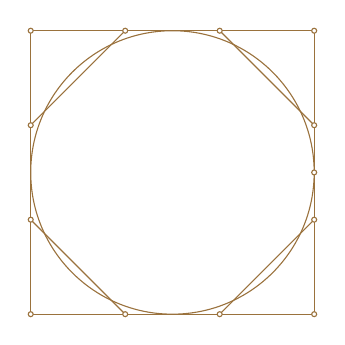
\begin{tikzpicture}[lichsutoanhoc, scale=0.6]
			\draw  (0.,0.) circle (3.cm);
			\draw  (-3.,-3.)-- (3.,-3.);
			\draw  (3.,-3.)-- (3.,3.);
			\draw  (3.,3.)-- (-3.,3.);
			\draw  (-3.,3.)-- (-3.,-3.);
			\draw  (1.,3.)-- (3.,1.);
			\draw  (3.,-1.)-- (1.,-3.);
			\draw  (-1.,-3.)-- (-3.,-1.);
			\draw  (-3.,1.)-- (-1.,3.);
				\draw [fill=white] (3.,0.) circle (1.5pt);
				\draw [fill=white] (-3.,-3.) circle (1.5pt);
				\draw [fill=white] (3.,-3.) circle (1.5pt);
				\draw [fill=white] (3.,3.) circle (1.5pt);
				\draw [fill=white] (-3.,3.) circle (1.5pt);
				\draw [fill=white] (1.,3.) circle (1.5pt);
				\draw [fill=white] (3.,1.) circle (1.5pt);
				\draw [fill=white] (3.,-1.) circle (1.5pt);
				\draw [fill=white] (1.,-3.) circle (1.5pt);
				\draw [fill=white] (-1.,-3.) circle (1.5pt);
				\draw [fill=white] (-3.,-1.) circle (1.5pt);
				\draw [fill=white] (-3.,1.) circle (1.5pt);
				\draw [fill=white] (-1.,3.) circle (1.5pt);
		\end{tikzpicture}
		\caption{\small\textit{\color{lichsutoanhoc}Hình $1$.}}
		\vspace*{-10pt}
	\end{figure}
	Trong bài toán khắc trên bảng đồng của người Babylon, số $\pi$  được chọn bằng $\dfrac{{25}}{8} = 3.125$.
	\vskip 0.1cm   
	Khi đo đạc tháp Gira vĩ đại ($2500$ trước Công nguyên), các nhà khảo cổ học đã nhận thấy người Ai Cập chọn số $\pi$  bằng $\dfrac{{22}}{7} \approx 3.14$.
	\vskip 0.1cm   
	Người Hebrews cũng lấy $\pi = 3$.  Điều này được thấy trong kinh Cựu ước, khi nói về bồn tắm tròn trong lâu đài của nhà vua Salomon. 
	\vskip 0.1cm
	\textbf{\color{lichsutoanhoc}Số Pi trong toán học Hy Lạp}
	\vskip 0.1cm
	Thuật toán đầu tiên tính gần đúng số $\pi$  được nhà toán học Hy Lạp Archimedes (khoảng $287-212$ trước Công nguyên) được trình bày trong cuốn sách  \textit{Measurement of the Circle} (\textit{Đo hình tròn}). Ông  đã tính được 
	\begin{align*}
		3\dfrac{{10}}{{71}} < \pi  < 3\dfrac{{10}}{{70}} \tag{$1$}
	\end{align*}
	bằng cách xét các đa giác đều $96$ cạnh nội tiếp và ngoại tiếp đường tròn như sau. 
	\vskip 0.1cm
	Giả sử $p_n$  và  $P_n$ là chu vi các đa giác đều $n$  cạnh nội tiếp và ngoại tiếp đường tròn chu vi $C$.  Khi ấy ta có 
	\begin{align*}
		{p_6} &< {p_{12}} < {p_{24}} < {p_{48}} < {\rm{ }}{p_{96}} < ... < {p_n} \\
		&< ... < C < ... < {P_n} < ... < {P_{96}} < {P_{48}} \\
		&< {P_{24}} < {P_{12}} < {P_6}.
	\end{align*}
	Dãy số $\{p_n\}$  là dãy số tăng, bị chặn trên bởi $C$  và $\{P_n\}$  là dãy số giảm bị chặn dưới bởi $C$.  Do đó chúng có giới hạn và có thể chứng minh giới hạn chung của chúng là  $C$.
	\vskip 0.1cm
	Giả sử  $Z$ là tâm hình tròn, và $AB = 2t$  và $CD = 2s$   tương ứng là độ dài một cạnh của đa giác đều $n$  cạnh ngoại tiếp và nội tiếp hình tròn. Gọi $M$  là điểm giữa của $AB$, $N$ là điểm giữa của  $CD$ và $O$  là giao điểm của tiếp tuyến tại điểm  $C$ với $MA$  (Hình $2$). Tương ứng $OM = OC = t'$  là nửa cạnh của đa giác đều $2n$  cạnh ngoại tiếp và $MC = MD = 2s'$ là cạnh của đa giác đều $2n$ cạnh nội tiếp đường tròn.     
	\begin{figure}[H]
		\vspace*{-5pt}
		\centering
		\captionsetup{labelformat= empty, justification=centering}
		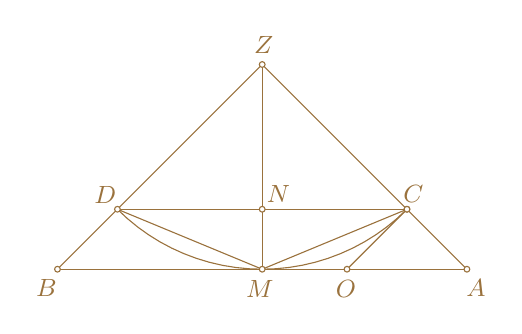
\begin{tikzpicture}[lichsutoanhoc,scale=1.3,node font= \small]
			\draw  (-1.414213562373095,-1.4142135623730954)-- (1.414213562373095,-1.414213562373095);
			\draw [shift={(0.,0.)},]  plot[domain=3.9269908169872414:5.497787143782138,variable=\t]({1.*2.*cos(\t r)+0.*2.*sin(\t r)},{0.*2.*cos(\t r)+1.*2.*sin(\t r)});
			\draw  (0.,0.)-- (-2.,-2.);
			\draw  (-2.,-2.)-- (2.,-2.);
			\draw  (2.,-2.)-- (0.,0.);
			\draw  (-1.414213562373095,-1.4142135623730954)-- (4.214684851089403E-8,-2.);
			\draw  (4.214684851089403E-8,-2.)-- (1.4142135623730958,-1.414213562373095);
			\draw  (0.8284271247461907,-2.)-- (1.4142135623730958,-1.414213562373095);
			\draw  (0.,0.)-- (4.214684851089403E-8,-2.);
				\draw [fill=white] (-2.,-2.) circle (0.8pt);
				\draw (-2.1070556519764487,-2.185112519201409) node {$B$};
				\draw [fill=white] (2.,-2.) circle (0.8pt);
				\draw (2.0884264234624923,-2.185112519201409) node {$A$};
				\draw [fill=white] (0.,0.) circle (0.8pt);
				\draw (0.01383926033153683,0.19322874030847648) node {$Z$};
				\draw [fill=white] (4.214684851089403E-8,-2.) circle (0.8pt);
				\draw (-0.02320693901008737,-2.1897168707627) node {$M$};
				\draw [fill=white] (0.,-1.4142135623730951) circle (0.8pt);
				\draw (0.15940855934397314,-1.2608345838502717) node {$N$};
				\draw [fill=white] (-1.414213562373095,-1.4142135623730954) circle (0.8pt);
				\draw (-1.5328395621812736,-1.2793576835210838) node {$D$};
				\draw [fill=white] (1.4142135623730958,-1.414213562373095) circle (0.8pt);
				\draw (1.477164134325693,-1.2608345838502717) node {$C$};
				\draw [fill=white] (1.414213562373096,-1.414213562373095) circle (0.8pt);
				\draw [fill=white] (0.8284271247461907,-2.) circle (0.8pt);
				\draw (0.8195940960118633,-2.194374069036815) node {$O$};
		\end{tikzpicture}
		\caption{\small\textit{\color{lichsutoanhoc}Hình $2$.}}
		\vspace*{-10pt}
	\end{figure}
	Vì $ACO$  và $AMZ$ là các tam giác vuông đồng dạng nên  $\dfrac{{t'}}{{t - t'}} = \dfrac{{OC}}{{OA}} = \dfrac{{ZM}}{{ZA}}.$
	\vskip 0.1cm
	Theo Định lý Thales ta có  $\dfrac{s}{t} = \dfrac{{NC}}{{MA}} = \dfrac{{CZ}}{{AZ}}.$
	\vskip 0.1cm
	Vì $MZ \in CZ$ nên ta có 
	\begin{align*}
		\dfrac{{t'}}{{t - t'}} = \dfrac{s}{t} \text{\color{black}\,\, hay } t' = \dfrac{{ts}}{{t + s}}.
	\end{align*}
	Vì các tam giác cân $CMD$  và  $COM$ là đồng dạng, nên ta có $\dfrac{{2s'}}{{2s}} = \dfrac{{t'}}{{2s'}},$  nghĩa là  $2{s'^2} = st'.$
	\vskip 0.1cm
	Vì $P_n$  và $p_n$  là chu vi đa giác đều $n$  cạnh, $P_{2n}$  và $p_{2n}$  là chu vi đa giác đều $2n$  cạnh ngoại và nội tiếp hình tròn nên ${p_n} = 2ns,$ ${P_n} = 2nt,$    ${p_{2n}} = 2ns',$   ${P_{2n}} = 2nt'.$
	\vskip 0.1cm
	Vậy $P_{2n}$   là trung bình điều hòa của  $p_n$ và $P_n$:
	\begin{align*}
		{P_{2n}} = 2nt' &= \dfrac{{2nts}}{{t + s}} = \dfrac{{2nt \cdot 2ns}}{{2nt + 2ns}} \\
		&= \dfrac{{{p_n} \cdot {P_n}}}{{{p_n} + {P_n}}}. \tag{$2$}
	\end{align*}
	Và $p_{2n}$ là trung bình nhân của $p_n$  và $P_{2n}$:  
	\begin{align*}
		{p_{2n}} = 2ns' &= 2n\sqrt {s \cdot t'}  = \sqrt {2ns \cdot 2nt'}  \\
		&= \sqrt {{p_n} \cdot {P_{2n}}} . \tag{$3$}
	\end{align*}
	Bắt đầu từ $n = 6$: $p_6 = 3d$ và $P_6 = 2\sqrt{3}d$,  trong đó $d$  là đường kính hình tròn, nhờ các công thức truy hồi ($2$) và ($3$), ta tìm được  $p_{96}$ và  $P_{96}$. Sử dụng đánh giá $\dfrac{{265}}{{153}}{\rm{ }} < \sqrt 3  < \dfrac{{1351}}{{780}}$,   Archimetdes tìm được tỷ số giữa chu vi đa giác đều $96$ cạnh và đường kính của hình tròn nội tiếp là 
	\begin{align*}
		14688:4673\dfrac{1}{2} = 3 + \dfrac{{667\dfrac{1}{2}}}{{4673\dfrac{1}{2}}} < 3\dfrac{1}{7} = 3\dfrac{{10}}{{70}}.
	\end{align*}
	Và tỷ số giữa chu vi đa giác đều $96$ cạnh và đường kính của hình tròn ngoại tiếp là
	\begin{align*}
		6336:2077\dfrac{1}{4} > 3\dfrac{{10}}{{71}}.
	\end{align*}
	Vậy ($1$) được chứng minh.
	\vskip 0.1cm
	Ta cũng có thể tính toán cách khác như sau.
	\vskip 0.1cm
	Giả sử đường tròn tâm $O$  có bán kính bằng $1$. $AB$  là một cạnh của hình đa giác đều $n$  cạnh nội tiếp đường tròn, có độ dài là $s_n$. Trong tam giác $OAB,$ kẻ $OC$  vuông góc với $AB$ cắt đường tròn tại  $D$. Suy ra $AD$ và $BD$  là hai cạnh của đa giác đều  $2n$ cạnh, có độ dài là  ${s_{2n}}$  (Hình $3$).
	\begin{figure}[H]
		\vspace*{-10pt}
		\centering
		\captionsetup{labelformat= empty, justification=centering}
		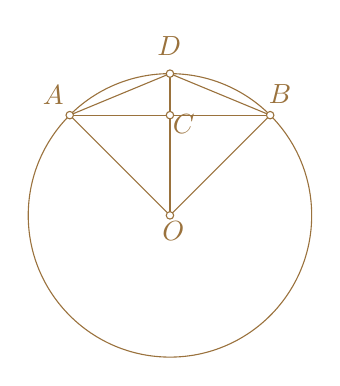
\begin{tikzpicture}[lichsutoanhoc,scale=0.9]
			\draw  (0.,0.) circle (2.cm);
			\draw  (-1.414213562373095,1.4142135623730954)-- (1.4142135623730954,1.4142135623730945);
			\draw  (-1.414213562373095,1.4142135623730954)-- (0.,0.);
			\draw  (0.,0.)-- (1.4142135623730954,1.4142135623730945);
			\draw  (0.,0.)-- (0.,2.);
			\draw  (0.,2.)-- (-1.414213562373095,1.4142135623730954);
			\draw  (0.,2.)-- (1.4142135623730954,1.4142135623730945);
			\draw [fill=white] (0.,0.) circle (1.5pt);
			\draw (0.046257928118391335,-0.21959254276378817) node {$O$};
			\draw [fill=white] (-1.414213562373095,1.4142135623730954) circle (1.5pt);
			\draw (-1.6467653276955618,1.696686527003653) node {$A$};
			\draw [fill=white] (1.4142135623730954,1.4142135623730945) circle (1.5pt);
			\draw (1.5532346723044377,1.7152911781664437) node {$B$};
			\draw [fill=white] (0.,1.414213562373095) circle (1.5pt);
			\draw (0.19509513742071688,1.2873842014222578) node {$C$};
			\draw [fill=white] (0.,2.) circle (1.5pt);
			\draw (-0.00955602536998075,2.3850586200269084) node {$D$};
		\end{tikzpicture}
		\caption{\small\textit{\color{lichsutoanhoc}Hình $3$.}}
		\vspace*{-10pt}
	\end{figure}
	Áp dụng định lý Pythagoras vào tam giác vuông $ACD$  ta có
	\begin{align*}
		A{D^2} = A{C^2} + C{D^2} = A{C^2} + {(OD - OC)^2}).
	\end{align*}
	Lại áp dụng định lý Pythagoras vào tam giác vuông $ACO$  ta được
	\begin{align*}
		OC = \sqrt {O{A^2} - A{C^2}} .
	\end{align*}
	Suy ra 
	\begin{align*}
		A{D^2} = A{C^2} + {\left( {OD - \sqrt {O{A^2} - A{C^2}} } \right)^2}
	\end{align*}
	Với  $OA = OD = 1,\;AC = \dfrac{{{s_n}}}{2},\;AD = {s_{2n}},$ ta có
	\begin{align*}
		&s_{2n}^2 = {\left( {\dfrac{{{s_n}}}{2}} \right)^2} + {\left( {1 - \sqrt {1 - {{\left( {\dfrac{{{s_n}}}{2}} \right)}^2}} } \right)^2}\\
		\Leftrightarrow &s_{2n}^2 = 2 - \sqrt {4 - s_n^2}.
	\end{align*}
	Suy ra 
	\begin{align*}
		{s_{2n}} = \sqrt {2 - \sqrt {4 - s_n^2} }. \tag{$6$}
	\end{align*}
	Sử dụng công thức ($4$), với hình lục giác đều có cạnh bằng bán kính và bằng $1$ (Hình $4$) ta được 
	\begin{align*}
		{s_{12}} = \sqrt {2 - \sqrt {4 - 1} }  = \sqrt {2 - \sqrt 3 } .
	\end{align*}
	Gấp đôi số cạnh được $n= 12$ thì 
	\begin{align*}
		{s_{24}} &= \sqrt {2 - \sqrt {4 - (2 - \sqrt 3 )} }  \\
		&= \sqrt {2 - \sqrt {2 + \sqrt 3 } } .
	\end{align*}
	Tiếp tục với $n = 24$  thì 
	\begin{align*}
		{s_{48}} = \sqrt {2 - \sqrt {2 + \sqrt {2 + \sqrt 3 } } } .
	\end{align*}
	Và với $n = 96$ thì ta được 
	\begin{align*}
		{s_{96}} = \sqrt {2 - \sqrt {2 + \sqrt {2 + \sqrt {2 + \sqrt 3 } } } } .
	\end{align*}
	\begin{figure}[H]
		\vspace*{-10pt}
		\centering
		\captionsetup{labelformat= empty, justification=centering}
		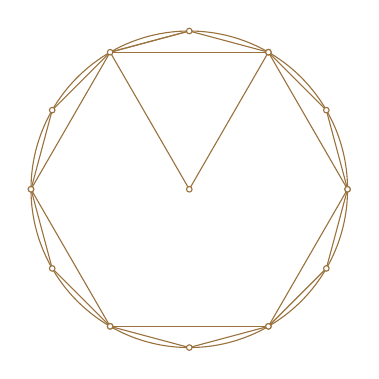
\begin{tikzpicture}[lichsutoanhoc,scale=0.67]
			\draw  (0.,0.) circle (3.cm);
			\draw  (-1.5,2.5980762113533165)-- (1.5,2.5980762113533165);
			\draw  (1.5,2.5980762113533165)-- (3.,0.);
			\draw  (3.,0.)-- (1.5,-2.5980762113533165);
			\draw  (1.5,-2.5980762113533165)-- (-1.5,-2.5980762113533165);
			\draw  (-1.5,-2.5980762113533165)-- (-3.,0.);
			\draw  (-3.,0.)-- (-1.5,2.5980762113533165);
			\draw  (0.,0.)-- (1.5,2.5980762113533165);
			\draw  (-1.5,2.5980762113533165)-- (0.,0.);
			\draw  (-1.5,2.5980762113533165)-- (0.,3.);
			\draw  (0.,3.)-- (-1.5,2.5980762113533165);
			\draw  (-1.5,2.5980762113533165)-- (-2.598076211353315,1.5);
			\draw  (-2.598076211353315,1.5)-- (-3.,0.);
			\draw  (-3.,0.)-- (-2.5980762113533165,-1.5);
			\draw  (-2.5980762113533165,-1.5)-- (-1.5,-2.5980762113533133);
			\draw  (-1.5,-2.5980762113533133)-- (0.,-3.);
			\draw  (0.,-3.)-- (1.5,-2.598076211353315);
			\draw  (1.5,-2.598076211353315)-- (2.598076211353314,-1.5);
			\draw  (2.598076211353314,-1.5)-- (3.,0.);
			\draw  (3.,0.)-- (2.5980762113533165,1.5);
			\draw  (2.5980762113533165,1.5)-- (1.5,2.5980762113533147);
			\draw  (1.5,2.5980762113533147)-- (0.,3.);
				\draw [fill=white] (0.,0.) circle (1.5pt);
				\draw [fill=white] (3.,0.) circle (1.5pt);
				\draw [fill=white] (-3.,0.) circle (1.5pt);
				\draw [fill=white] (-1.5,-2.5980762113533165) circle (1.5pt);
				\draw [fill=white] (1.5,2.5980762113533165) circle (1.5pt);
				\draw [fill=white] (-1.5,2.5980762113533165) circle (1.5pt);
				\draw [fill=white] (1.5,-2.5980762113533165) circle (1.5pt);
				\draw [fill=white] (0.,3.) circle (1.5pt);
				\draw [fill=white] (-2.598076211353315,1.5) circle (1.5pt);
				\draw [fill=white] (-3.,0.) circle (1.5pt);
				\draw [fill=white] (-2.5980762113533165,-1.5) circle (1.5pt);
				\draw [fill=white] (-1.5,-2.5980762113533133) circle (1.5pt);
				\draw [fill=white] (0.,-3.) circle (1.5pt);
				\draw [fill=white] (1.5,-2.598076211353315) circle (1.5pt);
				\draw [fill=white] (2.598076211353314,-1.5) circle (1.5pt);
				\draw [fill=white] (3.,0.) circle (1.5pt);
				\draw [fill=white] (2.5980762113533165,1.5) circle (1.5pt);
				\draw [fill=white] (1.5,2.5980762113533147) circle (1.5pt);
		\end{tikzpicture}
		\caption{\small\textit{\color{lichsutoanhoc}Hình $4$.}}
		\vspace*{-5pt}
	\end{figure}
	Chu vi của đa giác đều $96$ cạnh bằng
	\begin{align*}
		&96\cdot\dfrac{{{s_{96}}}}{2} \\
		= \,\,&48\cdot{s_{96}} = 48\sqrt {2 \!-\! \sqrt {2 \!+\! \sqrt {2 \!+\! \sqrt {2 \!+\! \sqrt 3 } } } }  \\
		\approx\,\, &3,14103 \approx 3\dfrac{{10}}{{71}}.
	\end{align*}
	Tương tự cho đa giác đều ngoại tiếp, ta có 
	\begin{align*}
		{S_{2n}} = \dfrac{{2\sqrt {4 + S_n^2}  - 4}}{{{S_n}}}. \tag{$5$}
	\end{align*}
	Bắt đầu với một lục giác đều ngoại tiếp một đường tròn (Hình $5$).  Do tam giác  $OAB$ đều nên 
	\begin{align*}
		OA = OB = AB = {S_6};\;\;AC = \dfrac{{{S_6}}}{2};\;\;OC = 1.
	\end{align*}
	Áp dụng định lý Pythagoras cho tam giác vuông $OAC$ ta có
	\begin{align*}
		O{A^2} = O{C^2} + A{C^2} &\Leftrightarrow S_6^2 = {1^2} + {(\dfrac{{{S_6}}}{2})^2} \\
		&\Leftrightarrow {S_6} = \dfrac{{2\sqrt 3 }}{3}.
	\end{align*}
	Theo ($5$) ta sẽ tính được ${S_{12}},{S_{24}},{S_{48}},{S_{96.}}$.
	Chu vi của đa giác đều $96$ cạnh là  
	\begin{align*}
		96.\dfrac{{{S_{96}}}}{2} \approx 3,14271 \approx 3\dfrac{{10}}{{70}}.
	\end{align*}
	\begin{figure}[H]
		\vspace*{-10pt}
		\centering
		\captionsetup{labelformat= empty, justification=centering}
		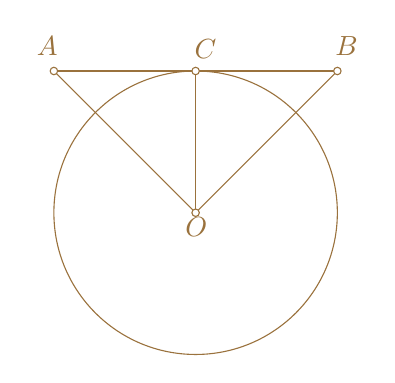
\begin{tikzpicture}[lichsutoanhoc,scale=0.9]
			\draw  (0.,0.) circle (2.cm);
			\draw  (-2.,2.)-- (0.,0.);
			\draw  (0.,0.)-- (2.,2.);
			\draw  (-2.,2.)-- (2.,2.);
			\draw  (0.,2.)-- (0.,0.);
			\draw [fill=white] (0.,0.) circle (1.5pt);
			\draw (0.009048625792809947,-0.20098789160099748) node {$O$};
			\draw [fill=white] (2.,2.) circle (1.5pt);
			\draw (2.129978858350949,2.347849317701327) node {$B$};
			\draw [fill=white] (-2.,2.) circle (1.5pt);
			\draw (-2.093276955602539,2.347849317701327) node {$A$};
			\draw [fill=white] (0.,2.) circle (1.5pt);
			\draw (0.1392811839323448,2.3106400153757454) node {$C$};
		\end{tikzpicture}
		\caption{\small\textit{\color{lichsutoanhoc}Hình $5$.}}
		\vspace*{-10pt}
	\end{figure}
	Vì hình tròn bị giới hạn bới các đa giác đều nội tiếp và ngoại tiếp, nên ($1$) được chứng minh.
	Trong \textit{Plinthides and Cylinders}, Archimedes còn tính số Pi: 
	\begin{align*}
		\dfrac{{195888}}{{62351}} > \pi  > \dfrac{{211875}}{{67441}}
	\end{align*}
	hay 
	\begin{align*}
		3.14697 > \pi  > 3.1463911.
	\end{align*}
	Đánh giá này không chính xác vì $\pi  \approx 3.141592654$   nằm ngoài khoảng trên. 
	Một đánh giá tinh tế hơn được làm bởi Tannery 
	\begin{align*}
		\dfrac{{195882}}{{62351}} > \pi  > \dfrac{{211872}}{{67441}}
	\end{align*}
	hay 
	\begin{align*}
		3.141601578 > \pi  > 3.141590427.
	\end{align*}
	Một đánh giá khác là 
	\begin{align*}
		\dfrac{{195888}}{{62351}} > \pi  > \dfrac{{211875}}{{67444}}
	\end{align*}
	hay 
	\begin{align*}
		3.141697808 > \pi  > 3.141495166.
	\end{align*}
	Khoảng năm $150$ Công nguyên, nhà bác học Ptolemy, trong tác phẩm Almagest, dựa trên bảng tính các cung (Table of Chords), đã dùng biểu diễn gần đúng số Pi dưới dạng phân số trong hệ đếm cơ số $60$ là 
	\begin{align*}
		\pi  \approx 3 + \dfrac{8}{{60}} + \dfrac{{30}}{{{{60}^2}}} = \dfrac{{377}}{{120}} \approx 3.141666667.
	\end{align*}
	Ông cũng nhận xét rằng, số này nằm giữa $3\dfrac{{10}}{{71}}$  và  $3\dfrac{{10}}{{70}}.$
	\vskip 0.1cm
	\textbf{\color{lichsutoanhoc}Số Pi trong toán học Trung Quốc}
	\vskip 0.1cm
	Lúc đầu, người Trung Quốc chấp nhận xấp xỉ số $\pi \approx 3$. Đầu thế kỷ II, Trương Hành (張衡, khoảng $78-139$) tìm được  $\pi  \approx \sqrt {10}  \approx 3.162$. Bằng cách nội tiếp hình tròn bởi các hình lục giác đều và gấp đôi số cạnh, Liu Hui (劉徽, $220-280$) năm $263$ trong cuốn sách Cửu chương toán thuật (九章算術) đã tìm được $\pi  \approx 3.14$  và sau đó Ông tìm được  $\pi  \approx 3.14159.$ Tổ Xung Chi (祖沖之, $429-500$), sử dụng thuật toán của Liu Hui với đa giác $12288 = 3 \cdot {2^{12}}$  cạnh, đã tính số $\pi$  chính xác đến $8$ chữ số:
	\begin{align*}
		3.1415926 < \;\pi \; < 3.1415927\;
	\end{align*}
	Và Ông chọn $\pi \; \approx \dfrac{{\;355}}{{113}} \approx 3.1415929$
	hoặc  $\pi \; \approx \;\dfrac{{22}}{7} \approx 3.145927$. 
	\vskip 0.1cm
	\textbf{\color{lichsutoanhoc}Số Pi trong toán học Việt Nam}
	\vskip 0.1cm
	Lương Thế Vinh ($1441-1497$, [$4$]) và các nhà toán học sau ông, cho đến thế kỉ XVIII, chọn $\pi = 3$.  Nguyễn Hữu Thận ($1757-1831$, [$3$]) đã sử dụng giá trị của số $\pi$ gần đúng đến $8$ chữ số thập phân. Ông đã sử dụng số $\pi  \approx 3.14159265$,  trong khi sách \textit{Bút toán chỉ nam} của Nguyễn Cẩn in năm $1909$ [$1$], sau Nguyễn Hữu Thận $80$ năm vẫn dùng số  $\pi$  bằng $3.14$ hoặc $3.1416$. Tương tự, Phạm Gia Kỉ, trong \textit{Đại thành toán học chỉ minh} [$2$] viết khoảng $1840$ cũng chỉ dùng $\pi$  bằng $3.14$ hoặc $3.1416$.  Nguyễn Hữu Thận và Nguyễn Cẩn cũng nhắc đến \textit{cách tính của Tây phương} (phương pháp gấp đôi số cạnh của Archimedes). Quan hệ giữa đường kính và chu vi (thông qua số  $\pi$) được Nguyễn Hữu Thận gọi là \textit{định luật chu vi đường kính}. Nguyễn Hữu Thận phát biểu:
	\vskip 0.1cm
	\textbf{\color{lichsutoanhoc}Định luật chu vi đường kính}
	\vskip 0.1cm
	Đường kính $100000000$, chu vi $314159265$
	\vskip 0.1cm
	Lại có chu vi $p = 100000000$, đường kính $d = 31830988$.
	\vskip 0.1cm
	\textit{Giải thích.} Nếu lấy $\pi = 3,14159265$, đường kính $= 100000000$ thì chu vi đường tròn là  $p = d.\pi = 314159265$ (chính xác đến $8$ chữ số).
	\vskip 0.1cm
	Nếu biết chu vi $p = 100000000$,  thì 
	\begin{align*}
		d = \dfrac{p}{\pi } = \dfrac{{1000000}}{{3.14159265}} \approx 31830988
	\end{align*}
	(chính xác đến $8$ chữ số).
	\vskip 0.1cm
	Nguyễn Hữu Thận viết: \textit{Phương pháp là cho bên trong hình tròn bao chứa hình vuông, lại từ bên ngoài hình tròn cắt hình vuông. Phép toán đến ức, vạn lần, tập trung tìm sẽ được vô số đầu mối. Trong ngoài đến tập hợp, trong là cạnh huyền chính, ngoài là đường thẳng được cắt. Cho đến vô số đường bao quanh hình tròn, gần giống như trực tuyến mà được số chu vi này, vốn xuất phát từ phép Tây là kỹ lưỡng nhất.}
	\vskip 0.1cm
	\textit{Giải thích}. Đây là phép tính chu vi đường tròn bắt đầu bằng hình vuông nội và ngoại tiếp, sau đó gấp đôi số cạnh (phương pháp của Liu Hui). 
	Gọi $d$ là đường kính hình tròn, bán kính $r = \dfrac{d}{2}$. Chu vi hình vuông ngoại tiếp bằng $4d > \pi d = 3,14d$
	(cạnh hình vuông bằng đường kính). 	
	\begin{figure}[H]
		\vspace*{-5pt}
		\centering
		\captionsetup{labelformat= empty, justification=centering}
		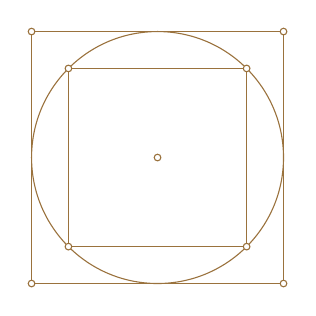
\begin{tikzpicture}[lichsutoanhoc,scale=0.8]
			\draw  (0.,0.) circle (2.cm);
			\draw  (-2.,-2.)-- (2.,-2.);
			\draw  (2.,-2.)-- (2.,2.);
			\draw  (2.,2.)-- (-2.,2.);
			\draw  (-2.,2.)-- (-2.,-2.);
			\draw  (-1.414213562373095,-1.4142135623730954)-- (1.414213562373095,-1.414213562373095);
			\draw  (-1.414213562373095,1.4142135623730954)-- (-1.414213562373095,-1.4142135623730954);
			\draw  (-1.414213562373095,1.4142135623730954)-- (1.4142135623730954,1.4142135623730945);
			\draw  (1.4142135623730954,1.4142135623730945)-- (1.414213562373095,-1.414213562373095);
				\draw [fill=white] (0.,0.) circle (1.5pt);
				\draw [fill=white] (-2.,-2.) circle (1.5pt);
				\draw [fill=white] (2.,-2.) circle (1.5pt);
				\draw [fill=white] (2.,2.) circle (1.5pt);
				\draw [fill=white] (-2.,2.) circle (1.5pt);
				\draw [fill=white] (-1.414213562373095,1.4142135623730954) circle (1.5pt);
				\draw [fill=white] (1.4142135623730954,1.4142135623730945) circle (1.5pt);
				\draw [fill=white] (-1.414213562373095,-1.4142135623730954) circle (1.5pt);
				\draw [fill=white] (1.414213562373095,-1.414213562373095) circle (1.5pt);
		\end{tikzpicture}
		\caption{\small\textit{\color{lichsutoanhoc}Hình $6$.}}
		\vspace*{-10pt}
	\end{figure}
	Hình vuông nội tiếp đường tròn có đường chéo bằng cạnh hình vuông bằng $\dfrac{d}{{\sqrt 2 }} = r\sqrt 2 .$ Do đó  chu vi hình vuông nội tiếp bằng (Hình $6$): $4r\; = 2d\; \approx 2d \times 1,4142 \approx 2,8284 < d\pi  \approx d.3,14 < 4d$.
	Gấp đôi số cạnh đa giác nội ngoại tiếp và tính giới hạn ta được chu vi hình tròn.
	Nguyễn Hữu Thận cũng phát biểu:
	\vskip 0.1cm
	\textbf{\color{lichsutoanhoc}Phép rút gọn chu vi, đường kính}
	\vskip 0.1cm 
	Đường kính: $113$	Chu vi: $355$
	\vskip 0.1cm
	Suy luận ban đầu là: Phép tính chu vi, đường kính, cách làm tốt dùng đường kính là $7$, đường bao quanh (chu vi) là $22$ thì thừa. Cách tỷ mỉ dùng đường kính là $50$, chu vi là $157$ thì thiếu. Chỉ có sắp đặt đường kính gộp lại là $113$, chu vi là $355$, phù hợp với định luật hơn. Cho nên chọn dùng nó.
	\vskip 0.1cm 
	\textit{Giải thích}. Chu vi hình tròn bằng:
	\begin{align*}
		p = d\pi  &\approx 7 \times 3.14159265 \\
		&\approx 21.99114855 < 22;\\
		p = d\pi  &\approx 50 \times 3.14159265 \\
		&\approx 157.0796325 > 157.\\
		d\pi  &\approx 113 \times 3.14159265 \\
		&\approx 354.99996945 < 355.
	\end{align*}
	Sai số:
	\vskip 0.1cm 		
	$1)$ $22 - 21.99114855 = 0.00885415$;  
	\vskip 0.1cm
	$2)$ $157.0796325 - 157 = 0.0796325$;
	\vskip 0.1cm
	$3)$ $355 - 354.99996 = 0,00004$
	($\dfrac{{355}}{{113}}$ chính xác nhất, đến $4$ chữ số).
	\vskip 0.1cm
	Vậy chọn $\pi  \approx \dfrac{{355}}{{113}}$ là phân số chính xác hơn cả. 
	\vskip 0.1cm
	Nguyễn Hữu Thận viết: \textit{Cạnh hình vuông với đường kính hình tròn bằng nhau nhưng diện tích hình vuông và diện tích hình tròn không có cùng định luật.}
	\vskip 0.1cm
	Diện tích hình vuông: $100000000$.
	\vskip 0.1cm	
	Diện tích hình tròn: $78539816$.
	\vskip 0.1cm
	Mặt khác:
	\vskip 0.1cm
	Diện tích hình tròn: $100000000$.
	\vskip 0.1cm 	
	Diện tích hình vuông: $127323954$.
	\vskip 0.1cm
	\textit{Giải thích.} Với cạnh $a = 10000$ thì diện tích hình vuông ${a^2} = 1.0000.0000$. Diện tích hình tròn nội tiếp hình vuông có đường kính bằng cạnh hình vuông, do đó 
	\setlength{\abovedisplayskip}{7pt}
	\setlength{\belowdisplayskip}{7pt}
	\begin{align*}
			S &= \pi {R^2} = \dfrac{{\pi {d^2}}}{4} = \dfrac{{\pi {a^2}}}{4}\\
			&\approx 3.14159265 \times 1.0000.0000:4 \\
			&\approx 78539816.	
	\end{align*}
	Nếu diện tích hình tròn là $100000000$ thì diện tích hình vuông là
	\begin{align*}
		{a^2} &= \dfrac{{4S}}{\pi } = \dfrac{{4 \times 100000000}}{{3.14159265}}\\ &= 127323954.
	\end{align*}
	Nguyễn Hữu Thận viết:  \textit{Diện tích hình vuông và diện tích hình tròn bằng nhau, cạnh hình vuông và đường kính hình tròn không cùng định luật.}
	\vskip 0.1cm
	Đường kính hình tròn: $100000000$.
	\vskip 0.1cm 
	Cạnh hình vuông: $88622692$.
	\vskip 0.1cm
	Lại có: 
	\vskip 0.1cm
	Cạnh hình vuông: $100000000$.
	\vskip 0.1cm 
	Đường kính hình tròn: $112837916$.
	\vskip 0.1cm
	\textit{Giải thích}. Diện tích hình vuông bằng diện tích hình tròn và bằng 
	\begin{align*}
		S &= \pi {R^2} = \dfrac{{\pi {d^2}}}{4}\\
		&\approx 3.14159265 \times {1.0000.0000^2}:4 \\
		&\approx 7853981633974483.
	\end{align*}
	Cạnh $a$ của hình vuông bằng
	\begin{align*}
		a = \sqrt S  \approx 88622692.
	\end{align*}
	Tương tự, nếu có cạnh hình vuông bằng $100000000$ thì  
	\begin{align*}
		d &= \sqrt {\dfrac{{4S}}{\pi }}  = \sqrt {\dfrac{{4{a^2}}}{\pi }}  = \dfrac{{2a}}{{\sqrt \pi  }} \\
		&\approx \dfrac{{2 \times 100000000}}{{\sqrt {3.14159265} }} \\
		&\approx 112837916.
	\end{align*}
	Như vậy, có thể khẳng định, Nguyễn Hữu Thận ($1757-1831$) là người Việt Nam đầu tiên có cảm nhận toán học về số vô tỷ và giới hạn thông qua quan hệ giữa số $\pi$ và diện tích các đa giác đều nội ngoại tiếp hình tròn khi gấp đôi số cạnh.
	\vskip 0.1cm
	\textbf{\color{lichsutoanhoc}Tiếp tục tính gần đúng số Pi}
	\vskip 0.1cm
	Tính toán thiên văn trong \textit{Shatapatha Brahmana} (Ấn Độ, thế kỉ IV trước Công nguyên) dùng xấp xỉ $\pi  \approx \dfrac{{339}}{{108}} \approx \;3.139$.  Một số tư liệu cổ của Ấn Độ chọn $\pi  \approx \sqrt {10}  \approx 3.162$. Trong tác phẩm \textit{Āryabhaṭīya}, nhà thiên văn Ấn Độ Aryabhata ($476-550$) đã sử dụng giá trị $\pi  = 3.1416$.
	\vskip 0.1cm 
	Fibonacci vào năm $1220$ đã tính được $\pi  = 3.1418$  độc lập với Archimedes. 
	\vskip 0.1cm
	Tác giả người Ý Dante đã sử dụng giá trị  $\pi  = 3 + \dfrac{{\sqrt 2 }}{{10}} \approx 3.14142.$
	\vskip 0.1cm 
	Mãi $8$ thế kỷ sau, kỷ lục của Tổ Xung Chi mới bị phá bởi nhà toán học Ba Tư Al--Kāshānī ($1370-1450$). Ông dùng phương pháp của Archimedes và xét các đa giác đều $3.2^{28}$ cạnh nội tiếp và ngoại tiếp đường tròn và tìm được số $\pi$ đúng với $17$ chữ số là $3.1415926535897932$.  Al--Kāshānī còn dự đoán $\pi$ là số vô tỷ. Điều này chỉ được chứng minh bởi nhà toán học Thụy Sĩ Johann Heinrich Lambert ($1728 - 1777$).
	\vskip 0.1cm 
	Cũng gấp đôi số cạnh như Archimedes, nhưng xuất phát từ hình vuông, nhà toán học Pháp François Viète vào năm $1578$ đã tính chính xác số $\pi$  đến $9$ chữ số nhờ sử dụng đa giác  $3 \times 2^{17}$ cạnh dựa trên công thức
	\begin{align*}
			\dfrac{2}{\pi } = &\cos \dfrac{\pi }{4} \cdot \cos \dfrac{\pi }{8} \cdot \cos \dfrac{\pi }{{16}}...\\
			= &\sqrt {\dfrac{1}{2}}  \cdot \sqrt {\dfrac{1}{2}\left( {1 + \sqrt {\dfrac{1}{2}} } \right)}  \\
			 &\!\times\!\sqrt {\dfrac{1}{2}\left( {1 \!+\! \sqrt {\dfrac{1}{2}\left(\! {1 \!+\! \sqrt {\dfrac{1}{2}} } \!\right)} } \right)} ... \tag{$6$}
	\end{align*}
	\textit{Giải thích}: Sử dụng công thức ${\cos ^2}a = \dfrac{{1 + \cos 2a}}{2}$  và $\cos \dfrac{\pi }{4} = \sqrt {\dfrac{1}{2}},$ ta dễ dàng tính được 
	\begin{align*}
		\cos \dfrac{\pi }{8} &= \sqrt {\dfrac{1}{2}\left( {1 + \sqrt {\dfrac{1}{2}} } \right)};\\
		\cos \dfrac{\pi }{{16}} &= \sqrt {\dfrac{1}{2}\left( {1 + \sqrt {\dfrac{1}{2}\left( {1 + \sqrt {\dfrac{1}{2}} } \right)} } \right)}.
	\end{align*}
	Công lao của François Viète là phát hiện ra công thức biểu diễn ($6$).
	\vskip 0.1cm
	Gọi $A(n)$  là diện tích đa giác đều $n$  cạnh nội tiếp hình tròn bán kính  $r$ và $\beta$ là góc ở tâm.  Ta có (Hình $2$):
	\begin{align*}
		A(n) = n\dfrac{1}{2}{r^2}\sin 2\beta  = n{r^2}\sin \beta \cos \beta .
	\end{align*}
	Tương tự,  
	\begin{align*}
		A(2n) = 2n\dfrac{1}{2}{r^2}\sin \beta  = n{r^2}\sin \beta .
	\end{align*}
	Suy ra
	\begin{align*}
		\dfrac{{A(n)}}{{A(4n)}} = \dfrac{{A(n)}}{{A(2n)}}\cdot\dfrac{{A(2n)}}{{A(4n)}} = \cos \beta \cos \dfrac{\beta }{2}.
	\end{align*}
	Do đó,
	\begin{align*}
			\dfrac{{A(n)}}{{A({2^k}n)}} &= \dfrac{{A(n)}}{{A(2n)}}\cdot\dfrac{{A(2n)}}{{A(4n)}}...\dfrac{{A\left( {{2^{k - 1}}n} \right)}}{{A({2^k}n)}}\\
			&= \cos \beta \cos \dfrac{\beta }{2}...\cos \dfrac{\beta }{{{2^k}}}.
	\end{align*}
	Khi $k$  tiến tới $\infty$  thì $A({2^k}n)$  tiến tới diện tích hình tròn, nghĩa là $\mathop {\lim }\limits_{n \to \infty } A({2^k}n) = \pi {r^2}.$ Suy ra  
	\begin{align*}
		\pi {r^2} &= \dfrac{{A(n)}}{{\cos \beta \cos \dfrac{\beta }{2}...\cos \dfrac{\beta }{{{2^k}}}...}} \\
		&= \dfrac{{\dfrac{1}{2}n{r^2}\sin 2\beta }}{{\cos \beta \cos \dfrac{\beta }{2}...\cos \dfrac{\beta }{{{2^k}}}...}}.
	\end{align*}
	Vậy  
	\begin{align*}
		\pi  = \dfrac{{n\sin 2\beta }}{{2\cos \beta \cos \dfrac{\beta }{2}...\cos \dfrac{\beta }{{{2^k}}}...}}.
	\end{align*}
	Để được công thức ($6$), Viète đã chọn $n = 4$. Khi ấy $\beta  = \dfrac{\pi }{4}$  và 
	\begin{align*}
		\sin 2\beta  = \sin \dfrac{\pi }{2} = 1, \cos \beta  = \cos \dfrac{\pi }{4} = \dfrac{1}{{\sqrt 2 }}.
	\end{align*}
	Nhà toán học Đức Adriaan van Roomen ($1561-1615$) nhận được xấp xỉ số  $\pi$ đến $15$ chữ số vào năm $1593$.
	\vskip 0.1cm 
	Năm $1596$, nhà toán học người Hà Lan Ludolph van Ceulen ($1540-1610$) đã dành $50$ năm trong hơn $70$ năm của đời mình để tính số $\pi$   xấp xỉ đến $35$ chữ số.
	\vskip 0.1cm 
	Năm $1621$, nhà khoa học Đức Willebrord Snellius đã đạt được xấp xỉ số $\pi$  đến $34$ chữ số.
	\vskip 0.1cm
	Năm $1630$, nhà thiên văn người Áo Christoph Grienberger ($1561-1636$) đã tìm được số $\pi$ xấp xỉ đến $38$ chữ số bằng cách sử dụng đa giác đều  $10^{40}$ cạnh.
	\vskip 0.1cm 
	Năm $1654$, Christiaan Huygens đã nhận được xấp xỉ đên $10$ chữ số thập phân nhờ sử dụng phương pháp ngoại suy Richardson.  
	\vskip 0.1cm
	Kỉ lục Christoph Grienberger chỉ bị vượt qua và thuật toán Archimedes đi vào lịch sử khi năm $1699$, số  $\pi$ được tính gần đúng đến $71$ chữ số nhờ phân tích số  $\pi$ dưới dạng chuỗi lũy thừa. Từ đó, số $\pi$ được tính gần đúng nhờ công cụ giải tích. Điều này sẽ được trình bày chi tiết trong Phần $2$.
	\vskip 0.1cm 
	\textbf{\color{lichsutoanhoc}Biểu diễn số $\pmb{\pi}$  dưới dạng phân số liên tục}
	\vskip 0.1cm
	Số $\pi$  có thể biểu diễn dưới dạng phân số liên tục như sau: 
	\begin{align*}
		\pi  \!=\! 3 \!+\! \dfrac{1}{{7 \!+\! \dfrac{1}{{15 \!+\! \dfrac{1}{{1 \!+\! \dfrac{1}{{292 \!+\! \dfrac{1}{{1 \!+\! \dfrac{1}{{1 \!+\! \dfrac{1}{{1 \!+\! ...}}}}}}}}}}}}}}
	\end{align*}
	Cắt cụt phân số này ta lần lượt được  $\pi  \approx 3;$  $\pi  \approx 3 + \dfrac{1}{7} = \dfrac{{22}}{7};$ $\pi  = 3 + \dfrac{1}{{7 + \dfrac{1}{{15}}}} = 3 + \dfrac{{15}}{{106}} = \dfrac{{333}}{{106}};$ $\pi  = 3 + \dfrac{1}{{7 + \dfrac{1}{{15 + 1}}}} = 3 + \dfrac{{16}}{{113}} = \dfrac{{355}}{{113}},$
	là các phân số xấp xỉ số $\pi$ thường gặp trong lịch sử các dân tộc Tây--Đông.
	\vskip 0.1cm
	\textbf{\color{lichsutoanhoc}Thông tin tác giả}
	\vskip 0.1cm
	$\bullet$ Tạ Duy Phượng (PGS Toán học)
	\vskip 0.1cm
	$\bullet$ Đoàn Thị Lệ, Cung Thị Kim Thành (Thạc sĩ Hán Nôm)
	\vskip 0.1cm
	$\bullet$ Mai Văn Thu, Nguyễn Hoàng Vũ (Thạc sĩ Toán học)
	\vskip 0.1cm
	\textbf{\color{lichsutoanhoc}Tài liệu trich dẫn}
	\vskip 0.1cm
	[$1$]   阮菫 Nguyễn Cẩn ($1909$),  \textit{Bút toán chỉ nam}, Thư viện viện nghiên cứu Hán Nôm, Viện nghiên cứu Hán Nôm, VHv. $282$ và A.$1031$. Bản thảo bản dịch của Đoàn Thị Lệ, $2015$.
	\vskip 0.1cm
	[$2$] 范嘉紀  Phạm Gia Kỷ,  大成算學指明  \textit{Đại thành toán học chỉ minh}, Thư viện viện nghiên cứu Hán Nôm, Viện nghiên cứu Hán Nôm, A.$1555$. Bản thảo bản dịch của Phạm Hữu Lộc, $2019$.
	\vskip 0.1cm 
	[$3$]  阮 有 慎 Nguyễn Hữu Thận,  意齋算法一得錄  \textit{Ý Trai toán pháp nhất đắc lục} ($1829$), Thư viện Viện nghiên cứu Hán Nôm, Vhv.$1184$, A.$1336$, A. $982$, A.$1336$/a. Bản thảo bản dịch của Đoàn Thị Lệ và Cung Thị Kim Thành, $2015-2016$.
	\vskip 0.1cm 
	[$4$] 梁世榮  Lương Thế Vinh,  算法大成 \textit{Toán pháp đại thành}, Thư viện Viện nghiên cứu Hán Nôm, Ký hiệu: A.$2931$ và VHv. $1152$. Bản thảo bản dịch của Cung Thị Kim Thành, $2017$.
	\vskip 0.1cm
	[$5$] David M. Burton, \textit{The History of Mathematics, An Introduction}, Seventh Edition, McGraw Hill, $2011$, $819$ p.
	\vskip 0.1cm
	[$6$] Heinrich Dörrie, \textit{The $100$ Great Problems of Elementary Mathematics, Their History and Solution}, New York, Dover Publications, INC., $1965$.
	\vskip 0.1cm     
	[$7$] Thomas Heath, \textit{A History of Greek Mathematics}, Oxford at the Clarendon Press, $1921$, Volume $1$, $232-235$.
	\vskip 0.1cm
	[$8$] Lam Lay--Yong and Ang Tian--Se, Circle Measurements in Ancient China, \textit{Historia Mathematica}, $13$,  ($1986$), $325-340$.
	\vskip 0.1cm
	[$9$] A. Volkov, Calculation of $\pi$ in ancient China: From Liu Hui to Zu Chongzhi, \textit{Historia Scientiarum}, Vol. $4$ ($1994$), No $2$, $139-157$. 
	\vskip 0.1cm
	\hfill (\textit{Còn tiếp})
\end{multicols}
%	\newpage
%	
%	\setcounter{figure}{0}
%	 \thispagestyle{gocconone}
\pagestyle{gocco}
\everymath{\color{gocco}}
\graphicspath{{../gocco/pic/}}
\blfootnote{$^1${\color[named]{gocco}Trung tâm Quy hoạch và Điều tra tài nguyên -- môi trường biển khu vực phía Nam.}}
\begingroup
\AddToShipoutPicture*{\put(0,616){\includegraphics[width=19.3cm]{../bannergocco}}}
\AddToShipoutPicture*{\put(106,522){\includegraphics[scale=1]{../tieude2.pdf}}} 
\centering
\endgroup

\vspace*{185pt}
\begin{multicols}{2}
	``\textit{Biết giấu mình dưới chín lớp đất cũng bằng biết khuấy động chín tầng trời}". Khi bắt đầu bước vào mỗi cuộc chiến cân não, nhiệm vụ quan trọng của đôi bên không chỉ là tìm cách bắt Tướng đối phương mà còn cần phải bảo vệ sự an toàn của Tướng của mình bằng những cách khéo léo và thông minh nhất. Để trở thành người chơi cờ giỏi, ngoài khả năng điều động quân lực, uy hiếp tấn công lên trận địa đối phương, các kỳ thủ cần sở hữu một kỹ năng không kém phần quan trọng, đó chính là Phòng thủ.
	\vskip 0.1cm
	Tuy vậy, tâm lý khi lâm trận của mỗi người thường muốn giành lấy chiến thắng càng nhanh càng tốt, nóng lòng hình thành thế tiến công ngay từ ban đầu khiến cho đối phương không kịp trở tay. Và nếu quá chăm chú vào mặt trận tấn tấn công mà lơ là mặt trận phòng thủ, hoặc phòng thủ một cách sơ sài, thiếu kế hoạch theo quan niệm ``\textit{Tấn công là cách phòng thủ tốt nhất}" thì chắc chắn sẽ để lộ ra những yếu điểm chết người, không thể giành thắng lợi mà còn tạo cơ hội cho đối phương phản kích dễ dàng.
	\vskip 0.1cm
	Trong bài viết kỳ này, tác giả sẽ gửi đến những hình cờ điển hình để bạn đọc Pi có thể hiểu hơn về tầm quan trọng của kỹ năng phòng thủ: 
	\vskip 0.1cm
	$1$.	Hình $1$, Đỏ còn chiến Xe rất mạnh và được đi tiên Đen chỉ còn Mã, Chốt và Tượng, Đỏ đi những nước mang tính uy hiếp như sau:  
	\begin{figure}[H]
		\vspace*{-5pt}
		\centering
		\captionsetup{labelformat= empty, justification=centering}
		\includegraphics[width= 0.4\textwidth]{1}
		\caption{\small\textit{\color{gocco}Hình $1$.}}
		\vspace*{-10pt}
	\end{figure}
	$\pmb{1)}$	X$5-2$ M$3.5$\quad $\pmb{2)}$ X$2.6$ Tg$5.1$\quad $\pmb{3)}$ X$2/1$ Tg$5/1$\quad $\pmb{4)}$ X$2/1$ Tg$5.1$\quad $\pmb{5)}$ X$2/1$ M$5/7$\quad $\pmb{6)}$ X$2-3$ Tg$/1$\quad $\pmb{7)}$ X$3.1$ ($*$) Tg$.1$\quad $\pmb{8)}$ Tg$5.1$ M$3.5$ $(**)$  ($1/2$)
	\vskip 0.1cm
	\textit{$(*)$: Dựa vào sức mạnh tuyệt đối của Xe, Đỏ liên tục tung ra những đòn quấy rối cực kỳ khó chịu. Tương ứng với đó Đen cũng đưa ra những đáp trả rất chính xác.
	\vskip 0.1cm
	$(**)$: Nếu trong tình huống thông thường cũng với số lượng quân như vậy, Đỏ sẽ dễ dàng giành chiến thắng. Tuy nhiên với hình cờ cụ thể này, những quân của Đen đã có vị trí rất đẹp và vận dụng kỹ năng phòng thủ rất thuần thục, các quân liên kết một cách hợp lý, tạo ra bức tường không thể khoan phá. Ván đấu có kết quả hòa là hoàn toàn xác đáng.}
	\begin{figure}[H]
		\vspace*{-5pt}
		\centering
		\captionsetup{labelformat= empty, justification=centering}
		\includegraphics[width= 0.4\textwidth]{2}
		\caption{\small\textit{\color{gocco}Hình $2$.}}
		\vspace*{-10pt}
	\end{figure}
	$2.$ Hình $2$, đôi bên đang có quân lực như nhau, tuy nhiên Đỏ nắm lợi thế vì Xe Chốt đang áp sát, sẵn sàng lấy mạng Tướng đối phương bất cứ khi nào. Trong thế đi hậu liệu Đen có thể thủ hòa thành công ? Diễn biến tiếp theo của cuộc cờ như sau: 
	\vskip 0.1cm
	$\pmb{1)}$	X$4-6$ $(*)$ X$5-6$ \quad $\pmb{2)}$ Tg$4-5$ Tg$5-6$ $(**)$\quad $\pmb{3)}$ C$7-6$  X$6-8$ $(***)$\quad $\pmb{4)}$ X$6-5$ X$8-5$\quad $\pmb{5)}$ Tg$5-6$ X$5-4$\quad $\pmb{6)}$ Tg$6-5$ X$4/3$ $(****)$ ($1/2$)
	\vskip 0.1cm
	\textit{$(*)$: Với lợi thế đi tiên, Đỏ ngay lập tức bình Xe sang trục lộ $6$ hòng tạo điều kiện cho Chốt lộ $7$ xâm nhập cửu cung một cách dễ dàng hơn.
	\vskip 0.1cm
	$(**)$: Đen cũng không hề chịu thua kém, ngay lập tức bình Xe rồi bình Tướng qua trục còn lại chiếm con đường huyết mạch. 
	\vskip 0.1cm
	$(***)$: Mặc dù Đỏ có bình chốt áp sát, Đen vẫn bình tĩnh đưa Xe sang lộ $8$ -- một nước chờ đợi đầy kinh nghiệm. Nếu ở đây Đen vội vàng tấn Chốt nhằm tìm cơ hội đối công thì sẽ phải trả giá rất đắt, Đỏ đi X$4-5$, Đen thua ngay lập tức.
	\vskip 0.1cm
	$(****)$: Mặc dù Đỏ chỉ còn $1$ nước nữa là có thể bình Chốt tạo sát, nhưng Đen cũng có những nước đáp trả đầy mẫu mực. Đôi bên chỉ còn đơn Xe, ván đấu kết thúc với kết quả hòa.}
	\begin{figure}[H]
		\vspace*{-5pt}
		\centering
		\captionsetup{labelformat= empty, justification=centering}
		\includegraphics[width= 0.4\textwidth]{3}
		\caption{\small\textit{\color{gocco}Hình $3$.}}
		\vspace*{-10pt}
	\end{figure}
	$3.$ Hình $3$, Quân lực của Đỏ đang áp đảo nhưng Đen chỉ cần một nước nữa là có thể tạo ra sát cục. Trong tình thế cực kỳ nguy cấp, Đỏ đã liên tiếp tung ra những đòn phế quân để thủ hòa như sau:
	\vskip 0.1cm
	$\pmb{1)}$ Xt$.1$ S$5/4$\quad $\pmb{2)}$ X$6.2$ Tg$5.1$\quad $\pmb{3)}$ X$6-5$ Tg$5-6$\quad $\pmb{4)}$ M$5/3$ P$7/5$\quad $\pmb{5)}$ X$5/8$ $(*)$ P$7-4$\quad $\pmb{6)}$ P$3-6$ C$4-5$\quad $\pmb{7)}$ P$6-7$ C$5.1$ $(**)$\quad $\pmb{8)}$ P$7/5$ C$4-5$\quad $\pmb{9)}$ P$7-5$ $(***)$ ($1/2$)
	\vskip 0.1cm
	$(*)$: Trong thế không còn gì để mất, Đỏ đã liên tục bỏ quân, trước phế Xe, sau hiến Mã khiến cho Đen chưa thể kết thúc ván cờ. Tranh thủ thời gian quý báu đó, Đen lui về tiêu trừ Chốt $5$ của Đen và chiếm lấy vị trí đắc địa để phòng thủ.
	\vskip 0.1cm
	$(**)$: Dù đã mất quân Chốt quý giá, Đen vẫn đủ lực, sử dụng Pháo Chốt để tạo một đợt tấn công khác. Sau khi tấn Chốt chém Xe Đỏ, Đen tiếp tục dọa sát.
	\vskip 0.1cm
	$(***)$: Đen vẫn có những nước phòng thủ vô cùng hợp lý. Tuy vẫn còn một chút lợi thế nhưng chừng đó là chưa đủ để Đen giành chiến thắng.
	\vskip 0.1cm
	\textit{Chú thích}: C: Chốt, X: Xe, M: Mã, P: Pháo, Tg: Tướng, S: Sĩ, T: Tượng, t: trước.
	\vskip 0.1cm
	\textbf{\color{gocco}Câu đố kỳ này:}  Đôi bên sẽ vận dụng khả năng điều quân như thế nào để giữ vững trận địa trong những hình cờ đối công dưới đây (bên Đỏ được quyền đi trước)?
	\begin{figure}[H]
		\vspace*{-5pt}
		\centering
		\captionsetup{labelformat= empty, justification=centering}
		\includegraphics[width= 0.4\textwidth]{4}
		\caption{\small\textit{\color{gocco}Hình $4$.}}
		\vspace*{-10pt}
	\end{figure}
	\begin{figure}[H]
		\vspace*{5pt}
		\centering
		\captionsetup{labelformat= empty, justification=centering}
		\includegraphics[width= 0.4\textwidth]{5}
		\caption{\small\textit{\color{gocco}Hình $5$.}}
		\vspace*{-10pt}
	\end{figure}
\end{multicols}
\vspace*{-10pt}
{\color{gocco}\rule{1\linewidth}{0.1pt}}
\vskip 0.2cm
{\centerline{\LARGE\textbf{\color{gocco}LỜI GIẢI, ĐÁP ÁN}}}
\begin{multicols}{2}
	Như vậy, chỉ có thể có $3$ trường hợp không phân biệt được rõ ràng khi khảo sát $199$ công dân: không có công dân thông minh nào, có một người thông minh tự tin, và có hai người thông minh khiêm tốn. Trong cả $3$ phương án này tất cả các phiếu điều tra đều ghi “Một”.
	\vskip 0.1cm
	Giờ ta sẽ xem, người tới muộn sẽ đưa ra những câu trả lời nào trong mỗi tình huống được nêu ở trên, phụ thuộc vào mức độ thông minh và khiêm tốn của anh ta.
	\vskip 0.1cm
	\vspace*{5pt}
	\newcolumntype{M}[1]{>{\centering\arraybackslash}m{#1}}
	\resizebox{\columnwidth}{!}{\begin{tabular}{|M{1cm}|M{2.5cm}|M{2.5cm}|M{2.5cm}|}
		\hline
		&$0$ người thông minh tự tin $0$ người thông minh khiêm tốn &$1$ người thông minh tự tin $0$ người thông minh khiêm tốn & $0$ người thông minh tự tin $2$ người thông minh khiêm tốn\\
		\hline
		Ngốc ngếch	& \centering$1$	&\centering$1$	&$1$\\
		\hline
		Tự tin	&$1$& $2$	&$3$\\
		\hline
		Khiêm tốn	&$0$&	$1$&	$2$\\
		\hline
	\end{tabular}}
	Ta thấy rõ ràng là các câu trả lời “$1$” và “$2$” đều được gặp ở vài ô, có nghĩa là chúng không giúp gì được cho việc phân biệt các tình huống. Tuy nhiên các trả lời “$0$” và “$3$” lại gặp đúng một lần, và chúng cho phép đưa ra các kết luận duy nhất. Vì thế người tới muộn đã đưa ra một trong các câu trả lời đó. Trong trường hợp anh ta trả lời “$0$” thì trong thành phố có duy nhất $1$ công dân thông minh (là chính người tới muộn đó), còn trong trường hợp anh ta trả lời “$3$” thì đúng là trong thành phố có $3$ công dân thông minh ($2$ người khiêm tốn và $1$ người tự tin là anh tới muộn đó).
	\vskip 0.1cm
	Đáp số: $1$ hoặc $3$.
\end{multicols}





%	\newpage
	
%	\thispagestyle{empty}
%	\begingroup 
%	\AddToShipoutPicture*{\put(0,0){\includegraphics[width=19.3cm]{dovui.pdf}}}
%	\centering
%	\vspace*{0cm}
%	\endgroup
%	\newpage	
%	\pagestyle{empty}
\end{document} 


%	\setcounter{figure}{0}
%	\thispagestyle{doisongtoanhocnone}
\pagestyle{doisongtoanhoc}
\everymath{\color{doisongtoanhoc}}
\graphicspath{{../doisongtoanhoc/pic/}}
%\blfootnote{$^1$\color{doisongtoanhoc}Trung tâm Thông tin -- Tư liệu, Viện Hàn lâm Khoa học và Công nghệ Việt Nam.}
\begingroup
\AddToShipoutPicture*{\put(0,616){\includegraphics[width=19.3cm]{../bannerdoisong}}}
\AddToShipoutPicture*{\put(43,527){\includegraphics[scale=0.95]{../tieude.pdf}}}\centering
\endgroup

\vspace*{185pt}


\begin{multicols}{2}	
	Đại hội Toán học Quốc tế (International Congress of Mathematicians, sau đây sẽ viết tắt là ICM) là sự kiện khoa học quan trọng hàng đầu của các nhà toán học trên thế giới. Nhiều người trong chúng ta đã quen thuộc với Kỳ thi Olympic Toán quốc tế (IMO). Vậy ICM có gì giống và khác với IMO? Mục đích của ICM là gì? Những hoạt động chính tại một kỳ ICM là gì? ICM $2022$ có những dấu ấn gì đặc biệt? Chúng tôi sẽ thử giải đáp các câu hỏi này.
	\vskip 0.1cm
	$\pmb{1.}$ \textbf{\color{doisongtoanhoc}ICM có gì giống và khác với IMO?}
	\vskip 0.1cm
	Cũng giống như IMO, ICM là một hoạt động cộng đồng hướng đến mục tiêu phát triển sự quan tâm đến toán học. Có lịch sử lâu đời hơn IMO một chút, ICM đầu tiên được tổ chức từ năm $1897$ tại Z\"urich, Thụy Sĩ, nhưng trong khi IMO được tổ chức hầu như hằng năm, thì ICM được tổ chức bốn năm một lần. Nếu IMO tập trung vào việc giải các bài toán, thì ICM hướng đến trình bày những thành tựu nghiên cứu toán học đáng kể nhất gần đây. Không có sự khác biệt đáng kể giữa nghiên cứu toán học và giải các bài toán Olympic, vì cả hai công việc đều đòi hỏi kỹ năng giải quyết vấn đề. Chúng ta biết rằng có những bài toán mở nổi tiếng trong toán học, như  định lý lớn Fermat (là bài toán mở đến trước $1994$), giả thuyết về số nguyên tố sinh đôi, hay giả thuyết Riemann (cả hai hiện vẫn chưa được giải quyết). Những tiến bộ về các bài toán mở nổi tiếng, nếu có, cũng là một điểm nhấn quan trọng của những kỳ ICM. Nhưng so với việc thi olympic, có thể nói các nhà toán học có nhiều tự do hơn trong việc làm nghiên cứu của mình, họ không nhất thiết phải làm việc với một vấn đề có sẵn. Có những nhà toán học lớn theo đuổi một vấn đề  hàng năm, thậm chí hàng chục năm trời. Việc một nhà số học ngồi nghe một bài giảng hình học đại số, hay một nhà đại số dự một bài giảng vật lý toán, để mở mang kiến thức, cũng là một việc thường xảy ra và được ICM khuyến khích.
	\vskip 0.1cm
	$\pmb{2.}$ \textbf{\color{doisongtoanhoc}Vì sao cần tổ chức ICM?}
	\vskip 0.1cm
	Mục đích chính của ICM là để tạo điều kiện cho các nhà toán học từ khắp nơi trên thế giới gặp gỡ những chuyên gia hàng đầu, và để tôn vinh những thành tựu toán học nổi bật nhất gần đây.
	\vskip 0.1cm
	Các nhà toán học gặp gỡ nhau? Chẳng phải các nhà toán học chỉ cần có giấy bút (và máy tính) để làm việc đó sao? Đúng là phần lớn các nhà toán học  có thiên hướng lý thuyết,  không cần nhiều trang thiết bị để làm việc. Nhưng ngoài giấy bút và máy tính, họ cũng thường cần một người đồng nghiệp ăn ý để thử nghiệm những ý tưởng chợt đến, tranh cãi về một chứng minh trong một bài báo, hay đơn giản tán gẫu về trận bóng tối qua. 
	\vskip 0.1cm
	Như bất cứ ngành khoa học có truyền thống nào, toán học ngày càng đa dạng hóa và chuyên môn hóa cao độ, với rất nhiều phân ngành khác nhau. ICM đầu tiên năm $1897$ chỉ có năm tiểu ban, mỗi tiểu ban phụ trách một chuyên môn, gồm có số học và đại số, giải tích và lý thuyết hàm, hình học, cơ học và vật lý toán, lịch sử và thư mục toán học. Nửa thế kỷ sau, ICM $1958$ mới có tám tiểu ban\footnote{\color{doisongtoanhoc}Xem Guillermo P. Curbera, \emph{Mathematicians of the World, Unite!}, Wellesley, Massachusetts: A.K. Peters, Ltd ($2009$), trang $14$ và $141$.}. Đến ICM $2022$, ta có đến hai mươi tiểu ban: logic, đại số, hình học đại số và hình học phức, tôpô, lý thuyết Lie và các mở rộng, giải tích, động lực học, phương trình vi phân, vật lý toán... Mỗi tiểu ban ngày nay lại có nhiều tiểu mục nhỏ hơn, ví dụ tiểu ban đại số có bốn tiểu mục.  Ngay từ ICM năm $1908$ ở Rome, Poincar\'e đã nhận ra: ``Khi một khoa học càng phát triển, ta càng khó nắm bắt được toàn bộ khoa học đó. Từ đó người ta phải chia nhỏ khoa học ấy ra nhiều phần, và bằng lòng với việc chỉ quan tâm tới đúng một trong các phần đó, nói cách khác là phải chuyên môn hóa. Chuyên môn hóa quá sâu sẽ làm cản trở nghiêm trọng đến tiến bộ chung của khoa học (...) Chính nhờ những tương tác bất ngờ giữa các hướng nghiên cứu khác nhau mà khoa học mới có thể phát triển."\footnote{\color{doisongtoanhoc}``In proportion as the science develops, it becomes more difficult to take it in its entirety. Then an attempt is made to
		cut it in pieces and to be satisfied with one of these pieces -- in
		a word, to specialize. Too great a movement in this direction
		would constitute a serious obstacle to the progress of science. As I have said, it is by unexpected concurrences
		between its different parts that it can make progress." Xem The Mathematical Intelligencer, Tập $34$, số $2$ ($2012$), trang $15-29$.} Nhà toán học nổi tiếng Hoàng Tụy ($1927-2019$) sinh thời thường cảnh báo về nguy cơ của chủ nghĩa tỉnh lẻ, khi một nhà khoa học làm việc trong tinh thần bế quan tỏa cảng và khiến bản thân thui chột. Gặp gỡ và tương tác với những chuyên gia hàng đầu tại những sự kiện lớn như ICM là cách giúp một nhà khoa học ``mở con mắt hướng ra những bờ cõi khoa học nơi những người khác đang chiếm cứ, và buộc ta phải so sánh thành tựu của mình với họ, qua đó nhận ra ngôi làng mình đang sống nhỏ bé chừng nào", theo lời của Poincar\'e\footnote{\color{doisongtoanhoc}Tài liệu đã dẫn, trang $20$.}.
	\vskip 0.1cm
	$\pmb{3.}$ \textbf{\color{doisongtoanhoc}Hoạt động chính ở các ICM là gì?}
	\vskip 0.1cm
	Hoạt động chính của ICM là các bài giảng của các chuyên gia, và phần trao giải thưởng ghi nhận những thành tựu toán học cao nhất đã đạt được giữa hai kỳ đại hội. Các bài giảng của chuyên gia gồm hai loại là các bài giảng toàn thể (khoảng $20$ bài) và các bài giảng tiểu ban (khoảng 180 bài). Được đọc bài giảng tại một ICM là một vinh dự lớn, nếu ta biết rằng mỗi năm có khoảng gần một trăm nghìn công trình toán học được xuất bản trên các tạp chí chuyên ngành. Các giải thưởng được trao ở các kỳ ICM gần đây là huy chương Fields (cho nhà toán học trẻ xuất sắc), giải thưởng Nevanlinna (khía cạnh toán học trong tin học), giải Gauss (toán ứng dụng), huy chương Chern (những người có thành tựu toán học xuất chúng, không hạn chế tuổi tác), và giải Leelavati (phổ biến kiến thức và quảng bá toán học). Trong số này, huy chương Fields nói chung được coi là giải thưởng danh giá nhất.
	\vskip 0.1cm
	$\pmb{4.}$ \textbf{\color{doisongtoanhoc}Ai có thể giành được huy chương Fields?}
	\vskip 0.1cm
	Huy chương Fields được trao cho những nhà toán học dưới $40$ tuổi với thành tựụ xuất sắc và tiềm năng phát triển lớn. Nhìn vào những người đoạt huy chương Fields gần đây, ta thấy họ nói chung là những người tài năng, được đào tạo bài bản (có bằng tiến sĩ), và theo đuổi những lĩnh vực quan trọng hoặc những bài toán quan trọng trong một thời gian dài. Có lẽ cách chắc chắn nhất để \emph{không} giành được giải Fields là lao vào những bài toán nổi tiếng, nhiều người biết, như giả thuyết Collatz, hay giả thuyết Riemann, bằng tay không, không quan tâm đến việc tích lũy kiến thức và các kỹ thuật cơ bản dần dần. Những huy chương Fields, ngoài sự dũng cảm tấn công những vấn đề khó khăn, còn ghi dấu ấn cụ thể, thuyết phục với những bài báo với nhiều người đọc, được bình duyệt chặt chẽ, trên những tạp chí toán học uy tín. Thông thường họ đã có một công chúng rộng lớn, những ý tưởng của họ đã có ích lợi đáng kể cho công việc của nhiều người khác, \emph{trước khi} được vinh danh với huy chương Fields, chứ không phải ngược lại. Tất nhiên không có quy tắc chung cho những tài năng đặc biệt, họ thường  phá vỡ những quy tắc mà chúng ta coi như hiển nhiên.
	\vskip 0.1cm
	$\pmb{5.}$ \textbf{\color{doisongtoanhoc}Đại hội Toán học Quốc tế $2022$ có gì đặc biệt?}
	\vskip 0.1cm
	ICM $2022$ được tổ chức từ ngày mùng $6$ đến $14/7/2022$. Lễ trao các giải thưởng được tổ chức trực tiếp tại Helsinki, Phần Lan vào ngày $5/7$. Về hình thức, sau $125$ năm lịch sử, đây là lần đầu tiên chương trình khoa học của ICM được tổ chức theo hình thức trực tuyến. Tại ICM năm nay, huy chương Fields đã được trao cho Hugo Dominil--Copin (Pháp), June Huh (Hàn Quốc), James Maynard (Vương quốc Anh), và Maryna Viazovska (Ukraina). Đây đều là những tên tuổi hàng đầu của toán học đương đại, những người sẽ còn tiếp tục ảnh hưởng lâu dài đến toán học. Nếu bạn nghĩ một bài giảng toán học là đối cực của một tiểu thuyết hấp dẫn/một bộ phim hay? Mời bạn xem bài giảng hết sức sáng sủa với đoạn cao trào tuyệt vời của June Huh, một người làm toán (những bài toán không hề đơn giản!) với hồn thơ đặc biệt. Nếu bạn, sau khi sở hữu một cỗ máy tiêu diệt hàng loạt các loại bài toán khó muôn hình vạn trạng, nghĩ quảng bá toán học là một việc nhàm chán và không cần công phu gì? Mời bạn xem bài giảng của Nikolai Andreev (giải Leelavati $2022$) và trang mạng độc đáo của ông\footnote{\color{doisongtoanhoc}https://etudes.ru/}.
	\vskip 0.1cm
	Trong một thế giới còn rất nhiều xung đột và đối kháng, các kỳ ICM và Liên đoàn Toán học Quốc tế (IMU) hướng đến gắn kết con người bằng toán học và tinh thần quốc tế, vượt qua những giới hạn về tư tưởng, ngôn ngữ, văn hóa, mặc cảm thượng đẳng/mặc cảm thấp kém thường ám ảnh con người. Từ khi kỳ ICM đầu tiên được tổ chức đến nay, toán học đã gánh chung tác động của hai thế chiến, chiến tranh lạnh, kỳ thị và phân biệt đối xử, với những hoạt động khác của con người. Vượt qua những khó khăn đó, cộng đồng toán học đã tiếp tục đi tới với lý tưởng bình đẳng, nhân văn, và chủ nghĩa quốc tế, di sản to lớn của những nhà toán học hàng đầu trong quá khứ. Chúng ta hy vọng vào thành công trong tương lai của toán học và của những lý tưởng này.
\end{multicols}

%	\newpage

%	\setcounter{figure}{0}
%	\thispagestyle{toanhocvadoisongnone}
\pagestyle{toanhocvadoisong}
\everymath{\color{toanhocdoisong}}
\graphicspath{{../toanhocdoisong/pic/}}
\begingroup
\blfootnote{$^1$\color{toanhocdoisong}Nguồn: Accromath, vol. $17$, $2022$.}
%\blfootnote{$^2$\color{toanhocdoisong}Đại học McGill, Canada.}
%\blfootnote{$^3$\color{toanhocdoisong}École Polytechnique Fédérale de Lausanne, Thụy Sỹ.}
\blfootnote{$^2$\color{toanhocdoisong}Viện Toán học.}
\blfootnote{$^3$\color{toanhocdoisong}Giải đấu để chọn ra người thách đấu với nhà vô địch -- Pi.}
\AddToShipoutPicture*{\put(0,616){\includegraphics[width=19.3cm]{../bannertoanhocdoisong}}}
\AddToShipoutPicture*{\put(102,507){\includegraphics[scale=1]{../tieude.pdf}}}
\centering
\endgroup

\vspace*{200pt}

\begin{multicols}{2}
	\textit{Khi các đấu thủ hoặc các đội thi đấu với nhau, cơ hội chiến thắng của mỗi bên phụ thuộc vào thực lực của họ. Hệ thống tính điểm Elo là một phương pháp tính toán trình độ tương đối của những người chơi trong một trò chơi có tổng bằng không, cho phép đánh giá khả năng về kết cục của một trận đấu.}
	\vskip 0.05cm
	Từ ngày $24$ tháng $11$ đến ngày $16$ tháng $12$ năm $2021$, tại Dubai đã diễn ra giải vô địch thế giới môn cờ vua. Kỳ thủ Nauy Magnus Carlsen, nhà vô địch từ năm $2013$, đấu với kỳ thủ Nga Ian Nepomniachtchi, người giành chiến thắng ở Giải đấu các ứng viên$^{\small{3}}$. Người chiến thắng giành được $1{,}2$ triệu euro tiền thưởng.
	\vskip 0.05cm
	Trận đấu gồm $14$ ván. Mỗi ván thắng được $1$ điểm, thua $0$ điểm và nếu hòa thì mỗi đấu thủ được $\frac{1}{2}$ điểm. Chung cuộc, Carlsen giành chiến thắng $7\frac{1}{2} - 3\frac{1}{2}$, với $4$ thắng, $0$ thua và $7$ hòa sau $11$ ván ($3$ ván cuối cùng không cần thiết vì không làm thay đổi kết quả cuối cùng). Và như vậy Carlsen giành danh hiệu vô địch thế giới lần thứ $5$ liên tiếp.
	\vskip 0.05cm
	Kết quả này phù hợp với hệ thống tính điểm Elo mà Liên đoàn Cờ vua Thế giới (FIDE) sử dụng từ năm $1970$ để đánh giá trình độ tương đối của các kỳ thủ. Quả thực, khi đó Carlsen được xếp hạng số một thế giới với số điểm Elo $2856$, trong khi đối thủ của anh, kỳ thủ số một của Nga, xếp thứ năm với số điểm Elo $2782$.
	\vskip 0.05cm
	Khi hai đấu thủ $A$ và $B$ với Elo $\theta_A$ và $\theta_B$ đấu với nhau, phương pháp Elo dự đoán $A$ sẽ giành được số điểm trung bình là
	\setlength{\abovedisplayskip}{4pt}
	\setlength{\belowdisplayskip}{5pt}
	\begin{align*}
		s_{AB} = \frac{1}{1+ 10^{-(\theta_A - \theta_B) /400}} \tag{$1$}
	\end{align*}
	biết rằng $A$ được $1$ điểm nếu thắng, $0$ nếu thua và $\frac{1}{2}$ nếu hòa. Điểm số trung bình B giành được là $s_{BA} = 1 – s_{AB}$.
	\vskip 0.05cm
	Trước trận tranh ngôi vô địch, ta có $\theta_A = 2856$ với Carlsen và $\theta_B = 2782$ với Nepomniachtchi, do đó $s_{AB} \approx 0{,}60$, tiên đoán chiến thắng của kỳ thủ Nauy vì trung bình anh sẽ giành được $8\frac{1}{2}$ điểm sau $14$ ván, so với số điểm $5\frac{1}{2}$ của kỳ thủ Nga.
	\vskip 0.05cm
	\textbf{\color{toanhocdoisong}Cơ sở toán học của phương pháp tính điểm Elo}
	\vskip 0.05cm
	Để xác định số điểm trung bình $s_{AB}$ của kỳ thủ $A$ khi đấu với kỳ thủ $B$, phương pháp ngây thơ là lấy số điểm trung bình của $A$ trong các trận đã đấu giữa hai người. Nhưng trong một trò chơi như cờ vua, phần lớn trong số hàng trăm nghìn người chơi chưa từng gặp nhau, và ngay cả khi họ đã từng gặp nhau, số trận họ đã đấu với nhau là quá ít để có một đánh giá chất lượng. Hệ thống tính điểm Elo giải quyết khó khăn này dựa vào một mô hình toán học cho phép xếp hạng các đấu thủ và qua đó ước tính kết quả có thể xảy ra khi họ đối đầu nhau.
	\vskip 0.02cm
	Biểu thức ($1$) lấy cảm hứng từ một mô hình được thiết lập từ những năm $1920$ bởi nhà toán học người Đức Ernst Zermelo và sau đó được cải tiến bởi nhà thống kê người Canada Ralph Bradley và người đồng nghiệp Milton Terry. Trong các công trình này, cũng như trong phần còn lại của bài viết, ta giả sử mọi ván đấu đều phân định thắng thua. Như vậy đây là một mô hình đơn giản hóa, nhất là đối với môn cờ vua, khi hòa là kết quả thường xảy ra nhất giữa các kỳ thủ đỉnh cao.
	\vskip 0.02cm
	Khi một ván đấu kết thúc với kết quả thắng $(1)$ hoặc thua $(0)$, điểm số trung bình chính là xác suất $p_{AB}$ để $A$ thắng $B$. Mô hình Bradley--Terry--Elo giả sử rằng xác suất này có dạng
	
	\vspace{-15pt}
	\begin{align*}
		p_{AB} = G(\theta_A - \theta_B)\tag{$2$}
	\end{align*}
	ở đó $G: \mathbb R \rightarrow (0, 1)$ là một hàm liên tục, tăng ngặt sao cho $G(x) + G(-x) = 1$ với mọi số thực $x$ và $G(x) \rightarrow 1$ khi $x \rightarrow \infty$. Một thí dụ về hàm như thế được cho trong Hình $1$. Ta có $p_{AB} + p_{BA} = G(\theta_A - \theta_B) + G(\theta_B - \theta_A) = 1$, không có kết quả hòa. Vì $G(0) = 1/2$, hai đấu thủ có trình độ ngang nhau có xác suất thắng như nhau; hiệu $\theta_A - \theta_B$ càng tăng thì xác suất để $A$ thắng càng lớn, và tiến tới giới hạn bằng $1$, nghĩa là chiến thắng chắc chắn của $A$.
	Lựa chọn phổ biến nhất của $G$ là luật logistic với tham số $\beta > 0$, được định nghĩa bởi
	
	\vspace{-15pt}
	\begin{align*}
		L(x) = \frac{ 1 }{ (1 + e^{-\beta x}) }\tag{$3$}
	\end{align*}
	với mọi $x \in \mathbb R$.
	\begin{figure}[H]
%		\vspace*{5pt}
		\centering
		\captionsetup{labelformat= empty, justification=centering}
		\includegraphics[width= 0.8\linewidth]{pic1}
		\caption{\small\textit{\color{toanhocdoisong}Hình $1$. Đồ thị hàm logistic $L(x)$ với $\beta = \ln(10) / 400$.}}
		\vspace*{-10pt}
	\end{figure}
	Chọn $G = L$ với tham số $\beta = \ln(10) / 400$, ta thu được công thức ($1$) mà FIDE sử dụng. Ban đầu, nhà vật lý người Mỹ gốc Hungary Arpad Elo, người đưa phương pháp mô hình hóa này vào thế giới cờ vua, sử dụng một hàm phân phối chuẩn, khi đó $s_{AB}$ không có công thức tường minh như trên.
	\vskip 0.05cm
	\textbf{\color{toanhocdoisong}Tính chất của mô hình xác suất}
	\vskip 0.05cm
	Mô hình Bradley--Terry--Elo có ưu điểm là nó cho phép xếp hạng tất cả người chơi của một trò chơi theo trình độ tương đối, ngay cả khi họ chưa từng đối đầu trực tiếp. Do đó, ta có thể dùng nó để dự đoán, đặc biệt là dựa vào các mô phỏng.
	Tuy nhiên, giả định rằng xác suất để $A$ thắng $B$ có dạng ($2$) không hề là một điều vô tình. Như đã đề cập, nó ngầm cho rằng không có ván hòa. Nếu có kết quả hòa, mô hình sẽ cần phải được điều chỉnh.
	\vskip 0.05cm
	Biểu thức ($2$) cũng ngầm giả định rằng kết quả một trận đấu giữa $A$ và $B$ chỉ phụ thuộc vào trình độ tương đối $\theta_A - \theta_B$. Đặc biệt, những yếu tố như đi trước (cầm quân trắng trong cờ vua), được nghỉ ngơi nhiều hơn đối thủ, hay thi đấu trước các cổ động viên không ảnh hưởng đến kết quả cuối cùng (một điều không hợp lý đối với thể thao chuyên nghiệp).
	\vskip 0.05cm
	Hơn nữa, cần phải hiểu rằng điểm số Elo của một đấu thủ không hề có giá trị nội tại: ý nghĩa của nó phụ thuộc vào điểm số Elo của các đối thủ, vì ta có thể cộng tất cả với cùng một hằng số tùy ý, hiệu số giữa chúng vẫn giữ nguyên. Tương tự, nếu ta nhân tất cả các Elo với một hằng số $c > 0$ và thay hàm $G(x)$ bởi $G(x / c)$, các xác suất thắng cũng không thay đổi.
	\vskip 0.05cm
	Trong trường hợp công thức ($1$), được biểu diễn trong Hình $1$ với các giá trị $\theta_A - \theta_B$ từ $-400$ đến $+400$, tham số $\beta$ được chọn sao cho chênh lệch $100$ điểm cho xác suất thắng $64\%$ đối với người mạnh hơn. Nếu chênh lệch là $200$ điểm, xác suất là $75\%$, và nó vào khoảng $91\%$ khi chênh lệch là $400$ điểm.
	\vskip 0.05cm
	Trong cờ vua, điểm Elo của hầu hết các kỳ thủ có trong xếp hạng của FIDE nằm trong khoảng từ $1000$ đến $3000$. Phân phối của chúng nói chung không đối xứng và thay đổi tùy theo từng nước. Hơn nữa, có nhiều phiên bản khác nhau của hệ thống xếp hạng, ngoài ra nó còn được điều chỉnh để áp dụng cho nhiều trò chơi và môn thể thao khác, trong đó có cờ vây, \textit{scrabble}, nhiều trò chơi trên mạng, bóng đá, tennis và khúc côn cầu trên băng.
	\vskip 0.05cm
	\textbf{\color{toanhocdoisong}Cập nhật xếp hạng}
	\vskip 0.05cm
	Tất nhiên là trình độ tương đối của các đấu thủ thay đổi theo thời gian. Một số người mạnh lên khi tích lũy thêm kinh nghiệm, một số khác yếu đi do tuổi tác, hoặc, trong trường hợp các môn thể thao đồng đội, do chấn thương, do giải nghệ hoặc do chuyển nhượng không tốt.
	\vskip 0.05cm
	Để thể hiện sự thay đổi này, phương pháp tính điểm Elo đưa ra một quy tắc cập nhật điểm xếp hạng sau mỗi trận đấu. Gọi $\theta_{A, n}$ và $\theta_{B, n}$ là điểm xếp hạng (Elo) của hai đấu thủ A và B ngay trước lần gặp nhau thứ $n$. Elo đề xuất rằng sau trận đấu này, chênh lệch $\theta_{A, n} - \theta_{B, n}$ được phân phối lại cho hai người theo ``độ bất ngờ" của kết quả và một số thực dương $k$, gọi là \textit{hệ số phát triển}.
	\vskip 0.05cm
	Gọi $s$ là kết quả của ván đấu giữa $A$ và $B$, với $s = 1$ nếu $A$ thắng, $s = 0$ nếu $A$ thua và $s = 1/2$ nếu ván đấu hòa. Elo mới của $A$ sẽ là
	\begin{align*}
		\theta_{A, n + 1} = \theta_{A, n} + k (s – s_{AB, n}),
	\end{align*}
	ở đó $s_{AB, n}$ là kết quả dự đoán được tính theo công thức ($1$) với các giá trị $\theta_{A, n}$ và $\theta_{B, n}$. Dễ thấy điểm số Elo của $A$ tăng nếu $s = 1$, và $s_{AB, n}$ càng nhỏ thì điểm số tăng càng nhiều. Như vậy, chiến thắng trước một đối thủ mạnh hơn thì có giá trị hơn. Tương tự, điểm số Elo của $A$ giảm khi thua, tức là khi $s = 0$. Cuối cùng, khi ván đấu hòa, điểm số Elo của $A$ tăng nếu điểm số Elo ban đầu của $B$ lớn hơn, tức là $s_{AB, n} < 1/2$.
	Đối với các kỳ thủ chuyên nghiệp, hệ thống tính điểm Elo cố định giá trị $k = 10$, do đó tại giải vô địch thế giới, mỗi ván thắng mang lại cho Carlsen $10 \times (1 – 0{,}60) \approx 4$ điểm Elo, trong khi mỗi ván hòa khiến anh mất $10 \times (0{,}5 – 0{,}60) \approx 1$ điểm. Sau giải đấu, điểm số Elo mới của anh là
	\begin{align*}
		2856 + 4 \times 4{,}0 - 7 \times 1{,}0 = 2865,
	\end{align*}
	trong khi đó điểm số Elo của Nepomniachtchi giảm từ $2782$ xuống $2773$.
	\vskip 0.05cm
	Các giá trị khác của $k$ được dùng cho các trình độ khác nhau của các kỳ thủ. Chẳng hạn, người ta dùng $k = 40$ cho các kỳ thủ mới chơi chưa quá $30$ ván hoặc các kỳ thủ trẻ dưới $18$ tuổi, giúp họ nhanh chóng đạt đến trình độ thực. Sau đó, $k$ được quy định bằng $20$ chừng nào điểm Elo của họ vẫn ở dưới $2400$.
	\vskip 0.05cm
	\textbf{\color{toanhocdoisong}Tính chất của phương pháp cập nhật}
	\vskip 0.05cm
	Trong trường hợp đặc biệt khi tất cả các ván đấu đều phân thắng bại, ta thấy rằng một cách tổng quát, phương pháp cập nhật mà Elo đề xuất sử dụng một hàm $M: \mathbb R \rightarrow (0, \infty)$ liên tục, giảm ngặt sao cho $M(x) \rightarrow 0$ khi $x \rightarrow \infty$. Hàm này cho phép cập nhật điểm xếp hạng của các đấu thủ $A$ và $B$ như sau.
	\vskip 0.05cm
	Nếu $A$ thắng:
	\begin{align*}
		&\theta_{A, n  +1} = \theta_{A, n} + M(\theta_{A, n} - \theta_{B, n}),\\
		&\theta_{B, n  +1} = \theta_{B, n} - M(\theta_{A, n} - \theta_{B, n}).
	\end{align*}
	Nếu $B$ thắng:
	\begin{align*}
		&\theta_{A, n  +1} = \theta_{A, n} - M(\theta_{B, n} - \theta_{A, n}),\\
		&\theta_{B, n  +1} = \theta_{B, n} + M(\theta_{B, n} - \theta_{A, n}).
	\end{align*}
	Trong công thức của FIDE, $M(x) = k L(-x)$ với mọi số thực $x$.
	\vskip 0.01cm
	Công thức cập nhật này có ý nghĩa tìm kiếm xác suất. Thực vậy, gọi $\theta_A$ và $\theta_B$ là trình độ tương đối thực sự nhưng chưa biết của hai đấu thủ $A$ và $B$. Giả sử $G(\theta_A - \theta_B)$ là xác suất thực sự để $A$ thắng $B$. Kỳ vọng của thay đổi xếp hạng của $A$ tại thời điểm $n$ được cho bởi biểu thức sau:
	\begin{align*}
		&M(\theta_{A, n} - \theta_{B, n}) G(\theta_A - \theta_B)\\
		 &- M(\theta_{B, n} - \theta_{A, n}) G(\theta_B - \theta_A).
	\end{align*}
	Nếu phương pháp cập nhật là tốt, ta mong muốn rằng kỳ vọng này bằng $0$ khi $\theta_{A, n} - \theta_{B, n} = \theta_A - \theta_B$. Do $M$ là hàm giảm, ta cũng hy vọng rằng sau ván đấu, hiệu $(\theta_{A, n + 1} - \theta_{B, n + 1}) - (\theta_A - \theta_B)$ gần $0$ hơn so với hiệu $(\theta_{A, n} - \theta_{B, n}) - (\theta_A - \theta_B)$.
	\vskip 0.01cm
	Lập luận tương tự cũng đúng đối với $B$, và ta có thể kiểm tra rằng những tính chất mong muốn này được đạt nếu các hàm $G$ và $M$ thỏa mãn, với mọi số thực $x$:
	\begin{align*}
		M(x) / M(-x) = G(-x) / G(x). \tag{$4$}
	\end{align*}
	Từ phương trình cân bằng này, với một chút nỗ lực, ta có thể chứng minh rằng với mỗi hàm $M$ cho trước, hàm $G$ duy nhất thỏa mãn được cho bởi
	\begin{align*}
		G(x) = \frac { M(-x) }{ M(x) + M(-x) },
	\end{align*}
	với mọi $x \in \mathbb R$.
	\vskip 0.01cm
	Do đó, quy tắc cập nhật mà Elo đề xuất ngầm cho rằng xác suất ban đầu là xác suất logistic, tức là $G = L$.
	\vskip 0.01cm
	Có một lưu ý tinh tế: nếu ta cố định hàm $G$ trước thì tồn tại vô số hàm $M$ thỏa mãn quan hệ ($4$). Thật vậy, với mọi hằng số $k > 0$, $M(x) = k G(-x)$ là một nghiệm. Nhưng ta cũng có thể chọn $M(x) = k G(-x) S(|x|)$, ở đó $S$ là một hàm thỏa mãn $S(0) = 1$ và $S(x) = S(-x)$ với mọi số thực $x$. Tất nhiên là hàm $S$ được chọn phải đảm bảo tính đơn điệu giảm của $M$.
	\vskip 0.05cm
	\textbf{\color{toanhocdoisong}Kết quả về sự hội tụ}
	\vskip 0.05cm
	Có thể liên hệ phương pháp cập nhật của Elo với thuật toán giảm gradient ngẫu nhiên trong học máy trong một mô hình hồi quy logistic.
	\vskip 0.05cm
	Ta hãy tưởng tượng có $N$ đấu thủ và trình độ của họ được biểu diễn bởi vector $(\theta_1, \dots, \theta_N)$ ẩn nhưng cố định. Ta cũng giả sử rằng ban đầu, ta có một ước lượng $(\theta_{1, 0}, \dots, \theta_{N, 0})$, và các đấu thủ sẽ tham gia một dãy vô hạn các ván đấu, mỗi ván diễn ra 
	\end{multicols}
	\vspace*{-8pt}
	\begin{tBox}
		\begin{wrapfigure}{l}{0.18\linewidth}
			\vspace*{-15pt}
			\centering
			\captionsetup{labelformat= empty, justification=centering}
			\hspace*{3pt}\includegraphics[width= 1.1\linewidth]{pic2}
			\caption{\small\textit{\color{toanhocdoisong}\hspace*{15pt}Arpad Elo.}}
			\vspace*{-20pt}
		\end{wrapfigure}
		Sinh ngày $25$ tháng $8$ năm $1903$ tại Egyházaskeszö, Áo--Hung trong một gia đình khiêm tốn, Arpad Elo (Élö Árpád trong tiếng Hungary) di cư sang Mỹ năm $1913$ cùng cha mẹ. Ông học vật lý tại Đại học Chicago, sau đó giảng dạy tại Đại học Marquette Milwaukee, Wisconsin.
		\vskip 0.05cm
		Ông là một kỳ thủ tài ba, từng tám lần vô địch bang và là chủ tịch Liên đoàn Cờ vua Mỹ từ $1935$ đến $1937$. Ông nổi tiếng thế giới vì đã đưa vào sử dụng hệ thống mang tên mình, được xây dựng trong những năm $1950$ sau khi hệ thống xếp hạng đầu tiên, do Kenneth Harkness phát triển, bị chỉ ra những nhược điểm. Phương pháp mới được FIDE thông qua vào năm $1970$, và Elo trở thành thành viên danh dự của tổ chức này từ năm $1981$.
		\vskip 0.05cm
		Một phân tích chi tiết đầu tiên về hệ thống tính điểm Elo (có khi bị viết sai thành ELO như thể một từ viết tắt) được chính Elo đưa ra trong cuốn sách năm $1978$ của mình, The Rating of Chessplayers, Past and Present. Ngày nay, phương pháp của ông là một phần không thể tách rời của thế giới cờ vua. Nó được dùng để xác định cách các kỳ thủ đối đầu với nhau tại các giải cờ vua trên toàn thế giới, và mọi kỳ thủ đều theo dõi sát sao sự thay đổi điểm số Elo của mình để đo mức độ tiến bộ và biết được thứ bậc của mình trong cờ vua.
		\vskip 0.05cm
		Arpad Elo qua đời ngày $5$ tháng $11$ năm $1992$ (thọ $89$ tuổi) tại Brookfield, Wisconsin.
		\vspace*{-3pt}
	\end{tBox}
	\begin{multicols}{2}
	giữa hai đấu thủ được chọn ngẫu nhiên theo phân phối đều. Cuối cùng, tưởng tượng rằng sau mỗi ván, vector trình độ được cập nhật theo phương pháp của Elo tại hai tọa độ $i$ và $j$ của hai đấu thủ vừa thi đấu.
	\vskip 0.05cm
	Dưới giả thiết các hàm $G$ và $M$ thỏa mãn các điều kiện đã nói đến ở trên, và hơn nữa $M$ có đạo hàm bị chặn, nhà toán học người Anh David Aldous đã chứng minh được rằng khi $n$ tiến ra vô cùng, dãy các vector $(\theta_{1, n}, \dots, \theta_{N, n})$ đạt đến một phân phối dừng. Liệu phân phối dừng này có phải là một xấp xỉ tốt của $(\theta_1, \dots, \theta_N)$ hay không vẫn là một câu hỏi lý thuyết mở, mặc dù nó đã được khẳng định bởi nhiều mô phỏng và thực tế hàng chục năm sử dụng hệ thống xếp hạng Elo của các kỳ thủ cờ vua.
	\vskip 0.05cm
	Trong khi đó, mặc dù kết quả hội tụ như của Aldous tạo niềm tin đối với phương pháp của Elo, chưa chắc đã tồn tại một vector ẩn $(\theta_1, \dots, \theta_N)$ phản ánh trình độ thực sự của các đấu thủ. Rốt cuộc thì các đấu thủ thay đổi theo thời gian, và các đội thể thao cũng liên tục thay đổi. Vector trình độ thực, nếu tồn tại, là một vector động.
	\vskip 0.05cm
	Thành công của phương pháp tính điểm Elo nằm ở khả năng theo được sự thay đổi này mà không phải phụ thuộc vào một mô hình ngẫu nhiên chính xác. Đây là một thực tế được xác nhận trong môn cờ vua, và trong cả nhiều tình huống khác, trong đó tham số $\beta$ và hệ số phát triển $k$ cần được lựa chọn một cách thích hợp.
	\vskip 0.05cm
	\textbf{\color{toanhocdoisong}Hệ thống Elo trong khúc côn cầu}
	\vskip 0.05cm
	Để minh họa phương pháp tính điểm Elo và khả năng dự đoán của nó ở ngoài môn cờ vua, ta hãy cùng xem xét ứng dụng của nó trong môn khúc côn cầu trên băng\footnote[4]{\color{toanhocdoisong}Accromath là tạp chí Canada, nơi khúc côn cầu trên băng là môn thể thao phổ biến nhất -- Pi.}, trong đó nhiều điều chỉnh đã được thực hiện để tận dụng kết quả của tất cả các trận trong vòng đấu thường và vòng đấu loại trực tiếp của giải National Hockey League (NHL) kể từ khi nó ra đời vào năm $1917$. Các dữ liệu này được lưu tại trang \url{hockey-reference.com}.
	\vskip 0.05cm
	Thí dụ, các nhà phân tích Ryan Best và Neil Paine của trang \textit{FiveThirtyEight} đề xuất một hệ thống xếp hạng Elo tính đến các tham số sau:
	\vskip 0.05cm
	$a)$ Mỗi đội có số diểm Elo ban đầu là $1380$.
	\vskip 0.05cm
	$b)$ Quy tắc cập nhật sử dụng hệ số phát triển $k = 6$.
	\vskip 0.05cm
	$c)$ Ta tính đến lợi thế sân nhà, tức là nếu hai đội có cùng Elo, đội chủ nhà có xác suất thắng là $57{,}1\%$ thay vì $50\%$.
	\vskip 0.05cm
	$d)$ Thay đổi điểm Elo tăng thêm $25\%$ đối với những trận loại trực tiếp.
	\vskip 0.05cm
	$e)$ Đầu mỗi mùa giải, điểm Elo của mỗi đội được tính lại, bằng
	\begin{align*}
		0{,}7 \!\times\!\text{điểm xếp hạng mùa trước} + 0{,}3 \!\times\!\! 1505.
	\end{align*}
	Như vậy, điểm số Elo trung bình của cả mùa giải dao động hàng năm xung quanh $1500$.
	\begin{figure}[H]
		\vspace*{-5pt}
		\centering
		\captionsetup{labelformat= empty, justification=centering}
		\includegraphics[width= 1\linewidth]{pic3}
		\caption{\small\textit{\color{toanhocdoisong}Hình $2$. Xếp hạng Elo của đội Montreal Canadiens từ năm $1917$ đến nay.}}
		\vspace*{-10pt}
	\end{figure}
	Ngoài ra, mô hình của Best và Paine tính đến cả hiệu số bàn thắng -- bàn thua của mỗi trận đấu và sự phụ thuộc lẫn nhau (hay tự tương quan) giữa các trận đấu liên tiếp.
	\vskip 0.05cm
	Hình $2$ cho thấy sự thay đổi của xếp hạng Elo của đội Montreal Canadiens theo mô hình của Best và Paine. Đỉnh cao nhất của đồ thị nằm ở nửa sau của thập niên $1970$, giai đoạn mà họ giành được bốn cúp Stanley\footnote[5]{\color{toanhocdoisong}Danh hiệu vô địch hàng năm của NHL -- Pi.}  liên tiếp.
	\vskip 0.05cm
	Ta cũng có thể thấy các đỉnh khác trong nửa sau thập niên $1940$ và giữa những năm $1990$, cũng như thời kỳ xuất sắc ổn định cuối những năm $1950$, khi họ vô địch năm lần liên tiếp (từ $1956$ đến $1960$). Trái lại, xếp hạng Elo của đội dao động quanh mức trung bình kể từ đầu những năm $2000$. Sự hiện diện của họ tại trận chung kết cúp Stanley năm $2021$, bởi vậy, có ít khả năng lặp lại trong tương lai gần.
	\vskip 0.05cm
	Vì xếp hạng Elo có tính tương đối, sẽ bổ ích hơn nếu ta so sánh sự thay đổi xếp hạng của các câu lạc bộ khác nhau. Hình $3$ so sánh các đội Montreal Canadiens (đường màu đỏ), Toronto Maple Leafs (xanh nước biển) và năm đội giành cúp Stanley từ $2008$ đến $2017$, gồm Boston Bruins (da cam), Detroit Red Wings (xanh lá cây), Chicago Blackhawks (đen), Los Angeles Kings (tím) và Pittsburgh Penguins (vàng).
	\begin{figure}[H]
		\vspace*{-10pt}
		\centering
		\captionsetup{labelformat= empty, justification=centering}
		\includegraphics[width= 1\linewidth]{pic4}
		\caption{\small\textit{\color{toanhocdoisong}Hình $3$. Xếp hạng Elo của bảy đội NHL từ $2008$ đến $2018$; đội vô địch mỗi năm từ $2008$ đến $2017$ được đánh dấu bằng hình tròn.}}
		\vspace*{-10pt}
	\end{figure}
	Trong Hình $3$, các đội vô địch được đánh dấu bằng hình tròn. Đội vô địch năm $2018$, Washington Capitals, không được xét đến trong hình. Có thể thấy rõ là đội hay nhất không phải lúc nào cũng vô địch.
	\vskip 0.05cm
	\textbf{\color{toanhocdoisong}Kết luận}
	\vskip 0.05cm
	Là một yếu tố không thể thiếu trong thế giới cờ vua đồng thời có thể được áp dụng cho các trò chơi hai người có tổng bằng không nói chung, hệ thống tính điểm Elo cho phép đánh giá trình độ tương đối của các đấu thủ ngay cả khi họ chưa từng đối đầu nhau. Sự cập nhật liên tục dần dần qua từng trận đấu đem lại một cách đơn giản và hiệu quả để nắm bắt quá trình thay đổi của các đấu thủ hoặc của các đội, như được minh họa trong thí dụ về NHL.
	\vskip 0.05cm
	\PIbox{\textbf{\color{toanhocdoisong}Xếp hạng Elo của các kỳ thủ cờ vua}
		\vskip 0.05cm
		Ngày nay, một người mới chơi có điểm số Elo khoảng $1000$, còn một người chơi nghiệp dư giỏi có điểm số Elo khoảng $2000$. Các đại kiện tướng quốc tế cần đạt được điểm số Elo tối thiểu $2500$. Nhóm này gần như trùng với nhóm các kỳ thủ chuyên nghiệp, ngày nay có hơn $1000$ người trên toàn thế giới. Cho đến nay chỉ có khoảng mười lăm kỳ thủ từng đạt đến mức điểm Elo $2800$ trong sự nghiệp của mình.
		\vskip 0.05cm
		Các phần mềm cờ vua cũng có xếp hạng điểm Elo. Chương trình tốt nhất hiện nay, Stockfish, có điểm số Elo khoảng $3700$, cho thấy trong cờ vua máy tính đã vượt xa con người như thế nào: xác suất $p_{AB}$ giữa Stockfish ($A$) và Magnus Carlsen ($B$) là khoảng $0{,}992\ldots$ (tức là trung bình $992$ trận thắng và $8$ trận thua cho máy tính sau $1000$ trận đấu không có hòa). Đó cũng là khoảng cách giữa Carlsen và một kỳ thủ nghiệp dư giỏi có điểm số Elo $2000$, mức đạt được bởi khoảng $30000$ người.
		\vskip 0.05cm
		Ta cũng có thể đặt câu hỏi liệu xếp hạng Elo có thể giúp so sánh các kỳ thủ thuộc các thời đại khác nhau. Chẳng hạn, một kỳ thủ có điểm Elo $2700$ trong thập niên $1980$ liệu có trình độ tương đương với một kỳ thủ có điểm Elo $2700$ ngày nay? Đây là một câu hỏi phức tạp, nhất là khi bản thân môn cờ vua cũng đã thay đổi. Chẳng hạn, các kỳ thủ, từ những người chuyên nghiệp đến những người nghiệp dư hăng hái nhất, đều dùng phần mềm để luyện tập. Nhưng người ta cũng quan sát được hiện tượng ``lạm phát", được gây ra bởi chính cách tính điểm Elo. Từ đầu những năm $2000$, điểm Elo trung bình của $50$ kỳ thủ mạnh nhất đã tăng hàng chục điểm, do đó điểm Elo cỡ $2700$ ở năm $2010$ rất có thể kém giá trị hơn so với ở năm $2000$.}
\end{multicols}
%	\newpage
